% Options for packages loaded elsewhere
\PassOptionsToPackage{unicode}{hyperref}
\PassOptionsToPackage{hyphens}{url}
%
\documentclass[
]{article}
\usepackage{lmodern}
\usepackage{amsmath}
\usepackage{ifxetex,ifluatex}
\ifnum 0\ifxetex 1\fi\ifluatex 1\fi=0 % if pdftex
  \usepackage[T1]{fontenc}
  \usepackage[utf8]{inputenc}
  \usepackage{textcomp} % provide euro and other symbols
  \usepackage{amssymb}
\else % if luatex or xetex
  \usepackage{unicode-math}
  \defaultfontfeatures{Scale=MatchLowercase}
  \defaultfontfeatures[\rmfamily]{Ligatures=TeX,Scale=1}
\fi
% Use upquote if available, for straight quotes in verbatim environments
\IfFileExists{upquote.sty}{\usepackage{upquote}}{}
\IfFileExists{microtype.sty}{% use microtype if available
  \usepackage[]{microtype}
  \UseMicrotypeSet[protrusion]{basicmath} % disable protrusion for tt fonts
}{}
\makeatletter
\@ifundefined{KOMAClassName}{% if non-KOMA class
  \IfFileExists{parskip.sty}{%
    \usepackage{parskip}
  }{% else
    \setlength{\parindent}{0pt}
    \setlength{\parskip}{6pt plus 2pt minus 1pt}}
}{% if KOMA class
  \KOMAoptions{parskip=half}}
\makeatother
\usepackage{xcolor}
\IfFileExists{xurl.sty}{\usepackage{xurl}}{} % add URL line breaks if available
\IfFileExists{bookmark.sty}{\usepackage{bookmark}}{\usepackage{hyperref}}
\hypersetup{
  pdftitle={Quantifying changes in the Distribution of Atlantic Cod and Yellowtail Flounder on Georges Bank},
  hidelinks,
  pdfcreator={LaTeX via pandoc}}
\urlstyle{same} % disable monospaced font for URLs
\usepackage[margin=1in]{geometry}
\usepackage{longtable,booktabs}
\usepackage{calc} % for calculating minipage widths
% Correct order of tables after \paragraph or \subparagraph
\usepackage{etoolbox}
\makeatletter
\patchcmd\longtable{\par}{\if@noskipsec\mbox{}\fi\par}{}{}
\makeatother
% Allow footnotes in longtable head/foot
\IfFileExists{footnotehyper.sty}{\usepackage{footnotehyper}}{\usepackage{footnote}}
\makesavenoteenv{longtable}
\usepackage{graphicx}
\makeatletter
\def\maxwidth{\ifdim\Gin@nat@width>\linewidth\linewidth\else\Gin@nat@width\fi}
\def\maxheight{\ifdim\Gin@nat@height>\textheight\textheight\else\Gin@nat@height\fi}
\makeatother
% Scale images if necessary, so that they will not overflow the page
% margins by default, and it is still possible to overwrite the defaults
% using explicit options in \includegraphics[width, height, ...]{}
\setkeys{Gin}{width=\maxwidth,height=\maxheight,keepaspectratio}
% Set default figure placement to htbp
\makeatletter
\def\fps@figure{htbp}
\makeatother
\setlength{\emergencystretch}{3em} % prevent overfull lines
\providecommand{\tightlist}{%
  \setlength{\itemsep}{0pt}\setlength{\parskip}{0pt}}
\setcounter{secnumdepth}{-\maxdimen} % remove section numbering
\usepackage{tikz} \usepackage{pdflscape}
\newcommand{\blandscape}{\begin{landscape}}
\newcommand{\elandscape}{\end{landscape}}
\newcommand{\beginsupplement}{\setcounter{table}{0}  \renewcommand{\thetable}{S\arabic{table}} \setcounter{figure}{0} \renewcommand{\thefigure}{S\arabic{figure}}}
\usepackage{booktabs}
\usepackage{longtable}
\usepackage{array}
\usepackage{multirow}
\usepackage{wrapfig}
\usepackage{float}
\usepackage{colortbl}
\usepackage{pdflscape}
\usepackage{tabu}
\usepackage{threeparttable}
\usepackage{threeparttablex}
\usepackage[normalem]{ulem}
\usepackage{makecell}
\usepackage{xcolor}
\ifluatex
  \usepackage{selnolig}  % disable illegal ligatures
\fi
\newlength{\cslhangindent}
\setlength{\cslhangindent}{1.5em}
\newlength{\csllabelwidth}
\setlength{\csllabelwidth}{3em}
\newenvironment{CSLReferences}[2] % #1 hanging-ident, #2 entry spacing
 {% don't indent paragraphs
  \setlength{\parindent}{0pt}
  % turn on hanging indent if param 1 is 1
  \ifodd #1 \everypar{\setlength{\hangindent}{\cslhangindent}}\ignorespaces\fi
  % set entry spacing
  \ifnum #2 > 0
  \setlength{\parskip}{#2\baselineskip}
  \fi
 }%
 {}
\usepackage{calc}
\newcommand{\CSLBlock}[1]{#1\hfill\break}
\newcommand{\CSLLeftMargin}[1]{\parbox[t]{\csllabelwidth}{#1}}
\newcommand{\CSLRightInline}[1]{\parbox[t]{\linewidth - \csllabelwidth}{#1}\break}
\newcommand{\CSLIndent}[1]{\hspace{\cslhangindent}#1}

\title{Quantifying changes in the Distribution of Atlantic Cod and Yellowtail Flounder on Georges Bank}
\author{David M. Keith\textsuperscript{1},
Jessica A. Sameoto\textsuperscript{1},
Freya M. Keyser\textsuperscript{1}, and
Irene Andrushchenko\textsuperscript{2}}
\date{}

\begin{document}
\maketitle
\begin{abstract}
Sustainably managing marine fisheries has long been recognized as a global priority which has proven difficult to achieve. The reasons sustainable fisheries management goals have not been achieved include various socio-economic, political, and scientific factors. Scientifically, one of the major challenges has been understanding how spatial and temporal heterogenity in processes impact the population dynamics of a stock. Fisheries science has spent a great deal of effort collecting data, both biological and environmental, which are inherently spatial and temporal in nature. Computational and statistical limitations have resulted in science products which do not fully utilize the spatio-temporal information contained in these data and tend to treat stocks as homogeneous entities. Fortunately, computational advances coupled with more accessible statistical methods have resulted in new methodologies which can harness the spatio-temporal information contained in these fisheries data. Here we develop temporally variable species distribution models for Yellowtail Flounder (\emph{Limanda ferruginea}) and Atlantic Cod (\emph{Gadus morhua}) on Georges Bank (GB) using a suite of static environmental covariates and presence-absence information from groundfish trawl surveys in Canada and the United States. These models indicate there are both seasonal and long term shifts in the distribution of both stocks. The average sea surface temperature (SST; average from 1997-2008) and depth were significant predictors of the distribution of both stocks throughout the year. Significant shifts in the distribution of both stocks occurs relatively frequently, with the distribution of Atlantic Cod observed to differ approximately every 5 years, while the Yellowtail Flounder distribution appears to fluctuate at least every 3 years. The core areas for both stocks shifts to the north and east throughout the study period. Much of this shift is due to the loss of the stocks from southern and western portions of GB. The seasonal distribution of Atlantic Cod and Yellowtail Flounder are relatively consistent throughout the late winter and spring, while in the fall the distribution of Atlantic Cod shifts towards the edge of the bank. For Atlantic Cod there has been a substainal decline in core area within the United States waters on Georges Bank while there has been little change in Canadian waters. In U.S. waters the Yellowtail Flounder core area declined rapidly in the late 1970s and early 1980s, but rebounded rapidly in the 1990s and early 2000s, while the core area was unchanged or slowly increased in Canadian waters over this time. These trends have resulted in an increase in the proportion of both stocks in Canadian waters in recent years. The models for both stocks were also relatively successful at predicting the likely location of the stock up to 3 years into the future, in addtion the simplified models which use only the random field for prediction performed as well as the models that included environmental covariates. Here we show how these models are able to provide novel insights into both seasonal and inter-annual variability in species distributions even without the use of environmental covariates. The incorporation of spatial information into science advice will improve our ability to sustainably manage these stocks.
\end{abstract}

\hypertarget{ref-intro}{%
\section{INTRODUCTION}\label{ref-intro}}

Sustainable management of marine fisheries has been recognized as a critical challenge facing society in the 21\textsuperscript{st} century (\protect\hyperlink{ref-cbdAichiBiodiversityTargets2018}{CBD 2018}). The issues facing sustainable fisheries management are multifaceted and include interactions between complex ecological, socio-economic, and political factors (\protect\hyperlink{ref-halpernAchievingTripleBottom2013}{Halpern et al. 2013}). For example, fisheries management regions were often delineated as a result of political or geographic considerations rather than biological or ecological rationale. As a result, the management of a species within a region can vary from situations in which the management encompasses only a subset of the total population of a species, to situations in which the majority of the stock is manged across a region with significant heterogeneity in the processes that drive the population dynamics (\protect\hyperlink{ref-cadrinDefiningSpatialStructure2020a}{Cadrin 2020}).

Accounting for spatial and temporal heterogeneity in the processes that drive a stocks population dynamics has long been recognized as a challenge in fisheries science (\protect\hyperlink{ref-rickerFurtherNotesFishing1944}{Ricker 1944}; \protect\hyperlink{ref-bevertonDynamicsExploitedFish1957}{Beverton and Holt 1957}; \protect\hyperlink{ref-hilbornQuantitativeFisheriesStock1992}{Hilborn and Walters 1992}). Many of the traditional fisheries methods developed, and still currently used to assess fisheries, require assumptions about the underlying spatial processes, these assumptions generally result in models that treat stocks as spatially homogeneous entities. (\protect\hyperlink{ref-bevertonDynamicsExploitedFish1957}{Beverton and Holt 1957}; \protect\hyperlink{ref-rickerComputationInterpretationBiological1975}{Ricker 1975}; \protect\hyperlink{ref-hilbornQuantitativeFisheriesStock1992}{Hilborn and Walters 1992}). Many of these assumptions were required because of computational and statistical limitations and has lead to science products that do not fully utilize the spatio-temporal information contained in the underlying data. Techniques, such as survey stratification, have been utilized in an effort to account for spatial heterogeneity and reduce uncertainty in the indices feeding these models (\protect\hyperlink{ref-smithAnalysisDataBottom1996}{Smith 1996}). In addition, indices have been developed that can measure the evenness of the spatial distribution of a stock, these indicies are typically used to quantify changes in spatial patterns over time (e.g. \protect\hyperlink{ref-reuchlin-hugenholtzPotentialSpatialDistribution2015}{Reuchlin-Hugenholtz et al. 2015}). These indices are an additional source of information providing a synoptic view of how distributions of paramters (e.g.~survey abundance or biomass) have changed over time, but they are unable to provide a detailed understanding of the spatial changes in these distributions.

Species distribution models (SDMs) were one of the earliest modelling frameworks developed to better understand spatial distributions and the processes that influence the observed patterns in species distributions (\protect\hyperlink{ref-grinnellOriginDistributionChestNutBacked1904}{Grinnell 1904}; \protect\hyperlink{ref-boxPredictingPhysiognomicVegetation1981}{Box 1981}; \protect\hyperlink{ref-boothBioclimFirstSpecies2014}{Booth et al. 2014}). These models use environmental data and species ecological information to map the occurrence probability (OP; or some measure of abundance) of a species across some land(sea)-scape; quantitative SDMs originated with attempts to predict terrestrial plant distributions (\protect\hyperlink{ref-boxPredictingPhysiognomicVegetation1981}{Box 1981}). In the marine realm, the influence of SDMs has increased rapidly in recent years; SDMs have been used in the development of Marine Protect Areas (MPAs) and MPA networks, to better understand the distribution of Species at Risk (SAR), and to predict the impact of climate change (\protect\hyperlink{ref-cheungApplicationMacroecologicalTheory2008}{Cheung et al. 2008}; \protect\hyperlink{ref-robinsonPushingLimitsMarine2011}{Robinson et al. 2011}; \protect\hyperlink{ref-sundbladEcologicalCoherenceMarine2011}{Sundblad et al. 2011}; \protect\hyperlink{ref-domischSpatiallyExplicitSpecies2019}{Domisch et al. 2019}; \protect\hyperlink{ref-mchenryProjectingMarineSpecies2019}{McHenry et al. 2019}).

Historically, SDMs often did not explicitly consider temporal changes in the relationship between the environment and the response of the species; these SDMs provided a snapshot in time based on available data (\protect\hyperlink{ref-elithSpeciesDistributionModels2009}{Elith and Leathwick 2009}). However, more sophisticated SDM frameworks have been developed in which the underlying relationships can vary in time and space, this has lead to more dynamic models which can provide improved predictions and more completely utilize the information contained within the data (\protect\hyperlink{ref-merowDevelopingDynamicMechanistic2011}{Merow et al. 2011}; \protect\hyperlink{ref-thorsonJointDynamicSpecies2016}{Thorson et al. 2016}; \protect\hyperlink{ref-martinez-minayaSpeciesDistributionModeling2018}{Martínez-Minaya et al. 2018}). The development of these new spatio-temporal SDM models have been made possible by a number of recent statistical and computational advances such as the implementation of the Laplace approximation (LA), Automatic Differentiation (AD), Stochastic Partial Differential Equations (SPDE), and Gaussian Markov Random Fields (GMRFs) in commonly used programming languages (\protect\hyperlink{ref-kristensenTMBAutomaticDifferentiation2016}{Kristensen et al. 2016}; \protect\hyperlink{ref-rueBayesianComputingINLA2016}{Rue et al. 2016}; \protect\hyperlink{ref-thorsonGuidanceDecisionsUsing2019}{Thorson 2019}). The complex spatio-temporal analytical problems associated with these advanced SDM models can now be solved in a fraction of the time required by traditional methods.

\hypertarget{georges-bank}{%
\subsubsection{Georges Bank}\label{georges-bank}}

Georges Bank (GB) has been home to some of the most productive fisheries in the world for centuries and is home to a wealth of natural resources (\protect\hyperlink{ref-backusGeorgesBank1987}{Backus and Bourne 1987}). In the 1960s and 1970s numerous countries had large unsustainable fisheries in the region, but with the expansion of territorial seas to 200 miles offshore in 1977, control of resource exploitation (e.g.~fisheries) on GB fell under the jurisdiction of the United States (U.S.) and Canada (\protect\hyperlink{ref-hallidayNorthAtlanticFishery1996}{Halliday and Pinhorn 1996}; \protect\hyperlink{ref-andersonHistoryFisheriesManagement1997}{Anderson 1997}). The final demarcation of the Canadian and U.S. territorial waters on GB was implemented with an International Court of Justice (ICJ) decision in 1984. Within three years of this decision both countries had independent groundfish surveys and each of these surveys covered the entirety of GB at different times of the year.

Historically, GB supported substantial groundfish fisheries including Atlantic Cod (\emph{Gadus morhua}), Atlantic Haddock (\emph{Melanogrammus aeglefinus}), Yellowtail Flounder (\emph{Limanda ferruginea}) and numerous other species (\protect\hyperlink{ref-andersonHistoryFisheriesManagement1997}{Anderson 1997}). As observed throughout the northwest Atlantic, the biomass of Atlantic Cod on GB declined significantly in the early 1990s and there has been little evidence for recovery of this stock since this collapse (\protect\hyperlink{ref-andrushchenkoAssessmentEasternGeorges2018}{Andrushchenko et al. 2018}). Between the 1970s and the 1990s, the biomass of Yellowtail Flounder on GB was low, but evidence for a rapid recovery of this stock in the early 2000s resulted in directed fisheries for several years. However, this recovery was short lived and the biomass of this stock has been near historical lows for the last decade (\protect\hyperlink{ref-legaultStockAssessmentGeorges2018}{Legault and McCurdy 2018}). While the biomass of Atlantic Cod and Yellowtail Flounder remains low, both Atlantic Haddock and Sea Scallop (\emph{Placopecten magellanicus}), the latter being one of the most lucrative fisheries on GB over the last two decades, have experienced unprecedented productivity during this time (\protect\hyperlink{ref-stokesburyEstimationSeaScallop2002}{Stokesbury 2002}; \protect\hyperlink{ref-hartSplitNotSplit2013}{Hart et al. 2013}; \protect\hyperlink{ref-dfoStockStatusUpdate2019a}{DFO 2019}; \protect\hyperlink{ref-finleyAssessmentHaddockEastern2019}{Finley et al. 2019}).

Here we use a recently developed statistical framework {[}R-INLA; \protect\hyperlink{ref-lindgrenBayesianSpatialModelling2015}{Lindgren and Rue} (\protect\hyperlink{ref-lindgrenBayesianSpatialModelling2015}{2015}); \protect\hyperlink{ref-rueBayesianComputingINLA2016}{Rue et al.} (\protect\hyperlink{ref-rueBayesianComputingINLA2016}{2016}); \protect\hyperlink{ref-bakkaSpatialModellingRINLA2018}{Bakka et al.} (\protect\hyperlink{ref-bakkaSpatialModellingRINLA2018}{2018}){]} to develop spatio-temporal species distribution models for two depleted groundfish stocks on GB (Atlantic Cod and Yellowtail Flounder). Our objectives were to use data from 3 groundfish surveys in the region to; 1) develop temporally variable species distribution models for these two species and explore whether these distributions were influenced by a suite of static environmental layers, 2) identify any long-term shifts in the distribution of these stocks, 3) identify any seasonal changes in the SDMs using survey data collected in the winter, spring and fall, and 4) use the SDMs to quantify any observed shifts in core area within Canadian and U.S. waters.

\hypertarget{ref-methods}{%
\section{Methods}\label{ref-methods}}

\hypertarget{study-area}{%
\subsection{Study area}\label{study-area}}

Georges Bank, located in the northwest Atlantic straddling the U.S.-Canada maritime border, is a 3-150 m deep plateau that covers approximately 40,000 km\textsuperscript{2} and is characterized by high primary productivity, and historically high fish abundance (\protect\hyperlink{ref-townsendNitrogenLimitationSecondary1997}{Townsend and Pettigrew 1997}). It is an eroding bank with no sediment recharge and covered with coarse gravel and sand that provides habitat for many species (\protect\hyperlink{ref-valentineSeaFloorEnvironment1991}{Valentine and Lough 1991}). Since the establishment of the ICJ decision in 1984, the Canadian and U.S. portions of GB have been largely managed separately by the two countries, though some collaborative management exists (Figure \ref{fig:Overview}).

\hypertarget{data}{%
\subsection{Data}\label{data}}

Survey data were obtained from the Fisheries and Oceans Canada (DFO) ``\emph{Winter}'' Research Vessel (RV) survey from 1987-2019 and the National Marine Fisheries Service (NMFS) ``\emph{Spring}'' and ``\emph{Fall}'' groundfish surveys from 1972-2019. The Winter survey on GB typically occurs in February and early March, the Spring survey typically occurs in April and May, while the Fall survey generally takes place between September and November. For all surveys only tows deemed \emph{successful} (Class 1 data) were used in this analysis. This resulted in 2590 tows from the Winter survey, 2393 tows from the Spring survey, and 2506 tows from the Fall survey.

\hypertarget{environmental-covariates}{%
\subsection{Environmental covariates}\label{environmental-covariates}}

A suite of 22 spatial environmental and oceanographic datasets were obtained for this analysis (Table \ref{tab:table-1}). To eliminate redundant variables, Variance Inflation Factors (VIFs) were calculated for all variables and any variables with VIF scores \textgreater{} 3 were removed. This procedure was repeated until no variables remained with a VIF score \textgreater{} 3 (\protect\hyperlink{ref-zuurProtocolDataExploration2010}{Zuur et al. 2010}). A Principal Component Analysis (PCA) was undertaken using the data from the associated station locations for each survey with variables excluded from the PCA if they showed no evidence for correlation with other variables or if they had very non-linear correlation patterns (Table \ref{tab:table-1}). The top 4 PCA components, accounting for at least 80\% of the variability in the data for a given survey, were retained and included as covariates for the models in addition to the retained environmental covariates (See Supplemental Figure \ref{fig:PCA}).

\hypertarget{statistical-analysis}{%
\subsection{Statistical Analysis}\label{statistical-analysis}}

A Bayesian hierarchical methodology was implemented using the INLA approach available within the R Statistical Programming software R-INLA (\protect\hyperlink{ref-lindgrenBayesianSpatialModelling2015}{Lindgren and Rue 2015}; \protect\hyperlink{ref-bakkaSpatialModellingRINLA2018}{Bakka et al. 2018}; \protect\hyperlink{ref-rcoreteamLanguageEnvironmentStatistical2020}{R Core Team 2020}). In recent years, R-INLA has seen a rapid increase in use to model species distributions in both the terrestrial and marine realms (e.g. \protect\hyperlink{ref-cosandey-godinApplyingBayesianSpatiotemporal2015}{Cosandey-Godin et al. 2015}; \protect\hyperlink{ref-leachModellingInfluenceBiotic2016}{Leach et al. 2016}; \protect\hyperlink{ref-boudreauConnectivityPersistenceLoss2017}{Boudreau et al. 2017}). This methodology solves stochastic partial differential equations on a spatial triangulated mesh; the mesh is typically based on the available data (\protect\hyperlink{ref-rueBayesianComputingINLA2016}{Rue et al. 2016}). The mesh used in this study included 6610 vertices and was extended beyond the boundaries of the data to avoid edge effects (Figure \ref{fig:Mesh}). Default priors were used for the analysis, except for the range and standard deviation hyperparameters used to generate the random fields, which were Penalized Complexity (PC) priors (\protect\hyperlink{ref-zuurBeginnerGuideSpatial2017}{Zuur et al. 2017}; \protect\hyperlink{ref-fuglstadConstructingPriorsThat2019}{Fuglstad et al. 2019}). The range PC prior had a median of 50 km with a probability of 0.05 that the range was smaller than 50 km. The standard deviation of the PC prior had a median of 0.5 with a probability of 0.05 that the marginal standard deviation was larger than 0.5.

For the INLA models, survey data up to 2016 were used (\emph{Winter} survey from 1987-2016, \emph{Spring} and \emph{Fall} surveys from 1972-2016). Survey data from 2017-2019 were excluded from the main analysis and used only as a testing dataset. For all analyses, the response variable was the probability of the survey detecting the stock of interest (Occurrence Probability, \(OP_{it}\)) and a \emph{Bernoulli} GLM was utilized within R-INLA. Cells with an estimated OP \(\geq\) 0.75 were considered the \emph{core area}. A dashboard has been developed that can be used to explore the effect of defining different OPs as \emph{core area} and is available at \url{https://github.com/Dave-Keith/Paper_2_SDMs/tree/master/Dashboard}.

\[ OP_{it} \sim Bernoulli(\pi_{it}) \]

\begin{align}
E(OP_{it}) = \pi_{it} \qquad and \qquad var(OP_{it}) = \pi_{it} \times (1-\pi_{it})
\end{align}

\[ logit(\pi_{it}) = \alpha + f(Cov_{i}) + u_{it} \]

\[ u_{it} \sim GMRF(0,\Sigma) \]

Each variable retained after the VIF analysis, along with each of the 4 PCA components, was added to the model individually. All continuous covariates were modelled using the INLA random walk \('rw2'\) smoother, which allows for non-linear relationships between the response and each covariate (\protect\hyperlink{ref-zuurBeginnerGuideSpatial2017}{Zuur et al. 2017}; \protect\hyperlink{ref-zuurBeginnerGuideSpatial2018}{Zuur and Leno 2018}). The continuous covariates were centred at their mean value and scaled by their standard deviation. Covariates that were highly skewed (e.g.~depth) were log transformed before being standardized. Due to low sample size of several of the levels the Sediment type (Sed ; data obtained from \protect\hyperlink{ref-mcmullen2014GISData2014}{McMullen et al. 2014}) these infrequent categories were amalgamated into one factor level that was represented by an \emph{Other} term, resulting in three levels for the Sediment covariate(\emph{Other}, \emph{Sand}, and \emph{Gravel-Sand}). Across the three surveys approximately 93\% of the survey tows were on the \emph{Sand} or \emph{Gravel-Sand} bottoms and 7\% were in the amalgamated \emph{Other} category.

Four spatial random field (\(u_{it}\)) models with differing temporal components were compared for each stock and each survey, these were a) a static random field (t = 1), b) independent random fields every 10 years, c) independent random fields every 5 years, and d) and independent random fields every 3 years. The independent random fields (options b through d) were set retroactively from the most recent year resulting in a shorter duration random field at the beginning of the time series whenever the field time period was not a multiple of the whole time series length (e.g.~the 10 year random fields for the Spring models were 2007-2016, 1997-2006, 1987-1996, 1977-1986, and 1972-1976). Models with the same covariate structure but different random fields were compared using WAIC, CPO, and DIC; the results for each of these metrics were similar and only the WAIC results are discussed further. In all cases, the static random field was an inferior model when compared to models with multiple random fields and the results discussed here are largely limited to the comparison of the 10/5/3 year random fields. For brevity we refer to the results from each random field as an \emph{era} (e.g.~the \emph{core area} estimated when using the 2012-2016 random field is the \emph{core area} during the 2012-2016 \emph{era}).

\hypertarget{model-selection-overview}{%
\subsubsection{Model Selection Overview}\label{model-selection-overview}}

Stage 1 model selection for the different covariate models was undertaken using the static random field by adding individual covariates. For this first analysis, covariates were retained if low WAIC scores were obtained. CPO and DIC results were similar to WAIC so only WAIC is discussed further; the model selection results are available in the supplement and the complete results can be found in the Model Output and Model Diagnostics sections of the interactive dashboard (\url{https://github.com/Dave-Keith/Paper_2_SDMs/tree/master/Dashboard}). For Atlantic Cod this analysis identified depth (DEP) and the average sea surface temperature between 1997 and 2008 (SST) as having low WAIC scores in 2 of the 3 surveys (data obtained from \protect\hyperlink{ref-greenlawGeodatabaseHistoricalContemporary2010}{Greenlaw et al. 2010}). For Yellowtail Flounder, DEP was identified as an informative covariate in all 3 surveys. In addition, SED, and the average chlorophyll concentration between 1997 and 2008 (CHL) were retained based on their low WAIC scores in the Fall survey. Given the low number of informative covariates DEP, SST, and CHL were all retained for both species in Stage 2 of model selection. In Stage 2 of model selection, the variables were added pairwise (e.g.~for Atlantic Cod the models included SST + DEP, DEP + CHL, and SST + CHL) for both stocks and again compared using WAIC using the 10-year random fields. In Stage 3 of covariate model selection, models with 3 covariates were tested based on the Stage 2 results. For Atlantic Cod a three term model that included additive terms for SST, DEP, and CHL was the most complex model tested. For Yellowtail Flounder, the most complex model included SST, DEP, and SED. In Stage 3, additional covariates were retained if the WAIC for that model resulted in an improvement of the WAIC of more than 2, as compared to the lowest WAIC for the more parsimonious model.

Model selection on the temporal random fields was done while holding the environmental covariate terms the same. Initial model selection for the random fields (10 and 5-year fields) was done using the Dep + SST model for both species in all seasons given the general support for the Dep + SST model identified in Stage 2 of covariate model selection. For both species this indicated that the 10-year field was inferior to the more flexible 5-year random fields. For Atlantic Cod, the 3 and 5-year random fields were compared using the Dep + SST (which was the covariate model with the lowest WAIC). For Yellowtail, the final step of the random field model selection used the Dep + SST + Sed model (which was the covariate model with the lowest WAIC) for the 3-year and 5-year random field comparison. Note that for Yellowtail Flounder the Dep + SST + Sed covariate model was not run with the 10 year random field and the Dep + SST covariate model was not run using the 3-year random fields in all three seasons, thus there were no results to show for these \emph{potential} models. The key model selection results are provided in the supplement and the full results can be found in the dashboard. For Atlantic Cod the \emph{Full Model} chosen included additive \emph{Dep} and \emph{SST} covariates and used a random field which changed every 5 years. For Yellowtail Flounder, the \emph{Full Model} chosen included additive \emph{Dep}, \emph{SST}, and \emph{Sed} covariates, the \emph{Winter} and \emph{Spring} models used a 3-year random field, while the \emph{Fall} model used a 5-year random field.

\hypertarget{model-prediction}{%
\subsection{Model Prediction}\label{model-prediction}}

A predictive grid with cells having an area of approximately 9.1 km\textsuperscript{2} was developed (See Supplemental Figure \ref{fig:mesh-grid}). The models were developed using data up to and including 2016. To obtain the predictions of the \emph{OP} for Cod, the \emph{Full Model} included additive \emph{Dep} and \emph{SST} terms and used the 5-year random field. For Yellowtail \emph{OP} predictions, the \emph{Full Model} included additive \emph{Dep}, \emph{SST}, and \emph{Sed} covariates, the models for the Winter and Spring used the 3-year random field, while the model for the Fall used the 5-year random field (see either the interactive dashboard or the Supplemental Figures \ref{fig:diag-1-fe}-\ref{fig:diag-rf} for model selection results). Each cell was intersected with average \emph{SST}, \emph{DEP}, and \emph{Sed} fields (see Supplemental Figure \ref{fig:SST-Dep-Sed} for the distribution of these environmental covariates) and the OP was estimated for each grid cell in each \emph{era} for Atlantic Cod and Yellowtail Flounder in the Winter, Spring, and Fall. The results using the predictive grid were used to calculate the size of the \emph{core area} (OP \(\geq\) 0.75) for each \emph{era}.

This predictive grid was used to calculate the centre of gravity (COG) of the \emph{core area} for each \emph{era}. The COG was calculated in the UTM coordinate system (EPSG Zone: 32619) using the easting (\emph{X}) and northing (\emph{Y}) for each cell identified as \emph{core area} (\emph{i}) in each \emph{era} (\emph{t}) and weighted by the \emph{OP} at each of these locations.

\begin{align} 
x_{t}^{cog} = \frac{\sum_{i=1}^{n} (X_{i,t} \times OP_{i,t})}{\sum_{i=1}^{n}OP_{i,t}} 
\end{align}

\begin{align}
y_{t}^{cog} = \frac{\sum_{i=1}^{n} (Y_{i,t} \times OP_{i,t})}{\sum_{i=1}^{n}OP_{i,t}}
\end{align}

The standard deviation around the mean COG in the X and Y direction was calculated as:

\begin{align}
\sigma_{cog,t}^{x} = \sqrt{\frac{ \sum_{i=1}^{n}OP_{i,t}} { [(\sum_{i=1}^{n}OP_{i,t})^2 - \sum_{i=1}^{n}OP_{i,t}^2] \times \sum_{i=1}^{n} (OP_{i,t}  \times (X_{i,t} - x_{t}^{cog})^2)}} 
\end{align}

\begin{align}
\sigma_{cog,t}^{y} = \sqrt {\frac{ \sum_{i=1}^{n}OP_{i,t}} { [(\sum_{i=1}^{n}OP_{i,t})^2 - \sum_{i=1}^{n}OP_{i,t}^2] \times \sum_{i=1}^{n} (OP_{i,t}  \times (Y_{i,t} - y_{t}^{cog})^2)}} 
\end{align}

To quantify the ability of these models to predict future spawning aggregations, data from the 2017-2019 surveys were used as a testing dataset. This analysis utilized the \emph{Full Models} to predict the \emph{OP} 1, 2, and 3 years into the future. In addition to the full models, an \emph{Intercept Model} which used only the temporally varying random field for prediction (i.e.~the model excluded all environmental covariates) was compared to the predictions from the \emph{Full Models} for 2017-2019. Both the model residual and the 2017-2019 predictive error were calculated for each year using RMSE, MAE, and SD. Given the similarity of the results only the RMSE is presented (full results are available in the dashboard).

\hypertarget{model-validation}{%
\subsection{Model Validation}\label{model-validation}}

Five fold cross validation was used to compare the out-of-sample predictive performance for a subset of the 5-year random field models: intercept only, SST (Atlantic Cod), DEP (Yellowtail Flounder), and DEP + SST. The Atlantic Cod model validation was performed using the Winter survey data, the Yellowtail Flounder validation used the Spring survey data. The data were \emph{randomly} divided into 5 subsets and trained using 4 of the subsets; the 5th dataset was treated as a testing dataset to determine how well the model was able to predict out-of-sample data. Model performance was measured by comparing the model residuals from the training data to the prediction error from the testing data. The metrics used for this comparison were Root Mean Squared Error (RMSE), Mean Average Error (MAE), and the standard deviation (SD), given the similarity of the results only the RMSE is presented (full results are available in the dashboard). A subset of models were chosen because of the computational demands of this validation procedure.

\hypertarget{ref-results}{%
\section{RESULTS}\label{ref-results}}

\hypertarget{distributional-shifts}{%
\subsection{Distributional Shifts}\label{distributional-shifts}}

For both stocks their core areas shifted towards the north and east throughout the study period, this was most noticeable when focusing on the core area (OP \(\geq\) 0.75; Figure \ref{fig:cog-hep}). For Atlantic Cod the shift in distribution of the core area occurred relatively rapidly in the 1990s and the centre of gravity (COG) of the core area has been relatively stable since this period (Figure \ref{fig:cog-hep}). In the 1970s and 1980s, core area was observed across the bank, however since the mid-1990s there is a clear shift in distribution with core area concentrated along the north-east of the bank mainly in Canadian waters (see Supplemental Figures \ref{fig:pf-winter-cod} -\ref{fig:pf-fall-cod}). In addition, in the Fall, Atlantic Cod has tended to be distributed along the northern edge of GB and the distribution of Atlantic Cod during this time likely includes the northern slope of the bank where there is limited survey coverage. The size of the core area has followed a similar temporal pattern as the distribution, with a rapid decline in the core area for Atlantic Cod occurring in the 1990s in the Winter and Spring (Figure \ref{fig:area-hep}). In the Fall the decline in the size of the core area was observed approximately a decade earlier than in the Winter or Spring and the core area has always been much smaller in the Fall (Figure \ref{fig:area-hep}). Given the location of the stock along the edge of the bank during the Fall it is likely that a substantial portion of the stock is located along the slope where survey coverage is limited (Figure \ref{fig:Overview}).

The Yellowtail Flounder shift in core area has, in large part, resulted from a reduction in the core area along the southern flanks of GB. The core area has been consolidated in a central region of GB that straddles the ICJ line dividing Canada and the U.S (Figure \ref{fig:cog-hep}). The COG of Yellowtail Flounder has been relatively stable both seasonally and between eras since the 1990s despite large changes in the size of the core area during this time. The trends in, and size of, the core area during the Spring and Fall have been very similar since the 1980s. In both seasons there were large increases in core area in the 1990s followed by a variable, yet generally increasing, size of core area more recently (Figure \ref{fig:area-hep}). In the Winter an area of similar location and size is observed, but the size of the core area in the Winter has been in decline since a period of increase in the 1990s (Figure \ref{fig:area-hep}).

For both stocks the changes in the size of the core area were larger in the U.S. than in Canadian waters (Figure \ref{fig:area-can-vs-us-hep}). In the U.S. the declines in the size of core area of Atlantic Cod occurred rapidly in the early 1990s in the Winter and Spring. In the Fall the loss of core area occurred approximately a decade earlier, although the size of the core area in the U.S. during the Fall was always substantially lower than in the Winter or Spring. In Canada there has been minimal change in the size of the core area in any of the seasons through time; the size of the core area in the Fall has tended to be lower than observed in the Winter or Spring (Figure \ref{fig:area-can-vs-us-hep}). The size of the core area of Yellowtail Flounder in the U.S. declined steadily throughout the 1970s and 1980s, this was followed by an increase in the 1990s and early 2000s (Figure \ref{fig:area-can-vs-us-hep}). In the last decade the size of the core area in the U.S. appeared to stabilize. In Canada the size of core area for Yellowtail Flounder throughout the 1970s and 1980s was variable and relatively low, but in the mid-1990s the size of the core area increased and has been relatively stable since the late 1990s (Figure \ref{fig:area-can-vs-us-hep}).

\hypertarget{environmental-covariates-1}{%
\subsection{Environmental Covariates}\label{environmental-covariates-1}}

The spatial fields for the three environmental variables retained by model selection are shown in Supplemental Figure \ref{fig:SST-Dep-Sed}. The average SST between 1997 and 2008 had the largest effect on the OP of Atlantic Cod; they were more likely to be found in regions of the bank with a lower SST (Figure \ref{fig:cod-fe}). For all 3 surveys the OP of Atlantic Cod declined rapidly in regions of the bank where the SST was above approximately 10°C (Figure \ref{fig:cod-fe}). Although the Dep relationship was also retained in the final Atlantic Cod model the effect of Dep on OP was substantially smaller than the SST effect. During the Winter and Spring the OP peaked between 70-82 m and declined slowly in shallower and deeper waters (Figure \ref{fig:cod-fe}). There was no clear relationship with Dep in the Winter.

For Yellowtail Flounder, Dep had the largest effect on OP, with Yellowtail Flounder most likely to be observed between depths of 66-75 m in each of the 3 surveys and the Dep effect on OP was highest during the Spring (Figure \ref{fig:yt-fe}). The average SST between 1997 and 2008 was also included in the final model for all three seasons, with Yellowtail Flounder OP generally declining as SST increased. The effect of SST was least pronounced in the Fall. The sediment type also had a significant influence on the OP for Yellowtail Flounder in the Winter and Fall, with Sand and Gravel-Sand having higher OPs than the Other sediment category, this difference is most notable during the Winter (Figure \ref{fig:yt-fe} and Supplemental Figure \ref{fig:diag-3-fe}).

\hypertarget{model-hyperparameters}{%
\subsection{Model Hyperparameters}\label{model-hyperparameters}}

The decorrelation range for Atlantic Cod was above 100 km throughout the year and was generally higher than that observed for Yellowtail Flounder (Figure \ref{fig:hyper-range-var-est}). The range was highest for Atlantic Cod in the Spring with an estimate of 218 (95\% CI:131-346) km while the range during the Winter spawning period was the lowest at 154 (95\% CI:99-227) km. In the Fall the estimate declined from the Spring; the range in this period may be influenced by a portion of the stock being located outside of the study domain and the stock being more concentrated in one area (Figure \ref{fig:hyper-range-var-est}). For Yellowtail Flounder, the lowest range was estimated in the Winter at 86 (95\% CI:63-109) km with the Spring and Fall range estimates being higher and somewhat more variable than the Winter range estimate. The range estimates of Yellowtail Flounder throughout the year were smaller and less variable than that observed with Atlantic Cod (Figure \ref{fig:hyper-range-var-est}). The uncertainty of these estimates precludes any statistical differences being observed between the seasons.

The standard deviation of the random field was lower for Atlantic Cod in the Winter and Spring than during the Fall (Figure \ref{fig:hyper-sd-var-est}), this is indicative of the increased clustering and the relatively small effect of the environmental covariates during the Fall for Atlantic Cod. The standard deviation of the random field is highest for Yellowtail Flounder in the Winter and the seasonal differences for Yellowtail Flounder are smaller than those observed with Atlantic Cod (Figure \ref{fig:hyper-sd-var-est}). The standard deviation of the Yellowtail Flounder field is higher than Atlantic Cod in the Winter and Spring, but lower in the Fall (Figure \ref{fig:hyper-sd-var-est}). The posteriors of other hyperparameters for both stocks in the Winter, Spring, and Fall are provided in Supplemental Figures \ref{fig:hyper-cod-winter-post} - \ref{fig:hyper-yt-fall-post}.

\hypertarget{validation-and-prediction}{%
\subsection{Validation and Prediction}\label{validation-and-prediction}}

The 5-fold cross validation indicated that each of the models used for 5-fold cross validation (intercept only, SST (Atlantic Cod), DEP (Yellowtail Flounder), and DEP + SST) were able to predict the distribution for both stocks without an increase in bias or a loss of accuracy (Figure \ref{fig:folds}). The mean error of the residuals for the validation training set predictions were similar to the error from the predicted test data and while the mean error of the test data was generally more variable, the estimates were centred on 0 and thus there was no evidence of bias in these predictions (Figure \ref{fig:folds}). The RMSE from the test and training data showed similar patterns for both stocks and most of the models, although for Yellowtail Flounder the RMSE for both the training and test data from the intercept only model was slightly lower than either of the models with covariates. This suggests that the inclusion of the environmental covariates may result in a small loss of out-of-sample prediction (Figure \ref{fig:folds}).

The models resulted in a slight loss of accuracy when predicting the spawning distributions of each stock 1, 2, and 3 years into the future (Figure \ref{fig:pred-17-19}), but the predictions were well below the RMSE associated with a model with no predictive ability (dashed line; Figure \ref{fig:pred-17-19}). For both stocks the 2018 data consistently had the lowest prediction accuracy with the models tending to predict individuals where none were observed. This is in agreement with observations of the survey biomass indices being near historic lows for both stocks in 2018 (\protect\hyperlink{ref-andrushchenkoAssessmentEasternGeorges2018}{Andrushchenko et al. 2018}; \protect\hyperlink{ref-legaultStockAssessmentGeorges2018}{Legault and McCurdy 2018}). Generally, the predictive error from these models were at the high end of the range of the model error estimates when data were available, this indicates that the predictions from these models cmay be able to predict the spatial OP patterns for both stocks up to 3 years into the future (Figure \ref{fig:pred-17-19}).

\hypertarget{discussion}{%
\section{DISCUSSION}\label{discussion}}

The SDMs developed here incorporate environmental, spatial, and multi-scale temporal information to partition dynamic changes which occur both inter and intra-annually from static environmental relationships. This framework enables a more in depth understanding of the impact of temporal shifts in species distributions than simpler aggregation based indices that are often used in fisheries science to indicate temporal shifts in a stocks distribution (e.g. \protect\hyperlink{ref-reuchlin-hugenholtzPotentialSpatialDistribution2015}{Reuchlin-Hugenholtz et al. 2015} and see Supplemental Figure \ref{fig:gini-index} showing the Gini index timeseries for Yellowtail Flounder and Atlantic Cod on Georges Bank for each survey). A general shift in the distributions of both species towards the east and north was identified, in both cases this shift was in large part due to the loss of \emph{core area} in the southern and western portion of GB (primarily in US waters). In addition, the analysis of surveys from different times of the year provided a snapshot of the seasonal changes in the distributions of the species; the Yellowtail Flounder distribution was relatively stable throughout the year, while Atlantic Cod moved towards the northeastern slope of GB during the fall. Finally, the models were able to predict the location of Atlantic Cod and Yellowtail Flounder during spawning up to 3 years in the future with only a modest loss of predictive ability. The SDMs developed here can be used to identify regions of consistently high and low probability of occurrence, quantify changes in the size of a \emph{core area} over time and between seasons (surveys), quantify how rapidly shifts in their distributions occur, and provide short term forecasts of the spatial OP patterns in future years.

The core area for Atlantic Cod collapsed rapidly in the early 1990s in unison with the collapse of Atlantic Cod (and other groundfish) stocks throughout the Northwest Atlantic (\protect\hyperlink{ref-bundySealsCodForage2009}{Bundy et al. 2009}). Since the collapse, the size of the core area has remained relatively consistent but has continued to slowly shift to the northeast with this shift more pronounced in the Fall. The loss of \emph{core area} from the warmer southern and western reaches of the bank have primarily been the reason for the apparent shift in the distribution of cod into Canadian waters. In more recent years, the Fall distribution of Atlantic Cod was likely located on the northeastern slope of the bank and outside of the core survey domains of these surveys.

This apparent northeastern shift of the stock over the course of this study suggests that the surveys may no longer be sampling the entirety of Atlantic Cod throughout the course of the year (i.e.~a higher proportion of the stock may now be located outside of the survey domain in the Fall than in the past). Each of the survey indices had been used as inputs to the Atlantic Cod stock assessment model for eastern GB Atlantic Cod (\protect\hyperlink{ref-andrushchenkoAssessmentEasternGeorges2018}{Andrushchenko et al. 2018}). However, this assessment model suffered from such significant retrospective patterns that the model was recently rejected; the results of this study are in agreement with the suggestion that the observed shift in the distribution of Atlantic Cod outside of the survey domain was a contributing factor to the model retrospective problems (\protect\hyperlink{ref-andrushchenkoAssessmentEasternGeorges2018}{Andrushchenko et al. 2018}). In addition, because the management of this stock is shared between Canada and the U.S., the observed shift in the core distribution to Canadian waters suggests that shared management policies, such as quota sharing agreements between the two jurisdictions, may require regular review (e.g. \protect\hyperlink{ref-tmgcDevelopmentSharingAllocation2002}{TMGC 2002}).

Yellowtail Flounder were more likely to be found on bottom types which included sand, in regions of the bank that historically had lower temperatures, and at depths between 66-75 meters; this is consistent with the known life history for this species (\protect\hyperlink{ref-johnsonYellowtailFlounderLimanda1999}{Johnson et al. 1999}). In addition, there was a consistent elevated likelihood of encountering Yellowtail Flounder in the region straddling the ICJ line which was not explained by the environmental covariates. This suggests this region has some unexplained ecological or environmental significance to Yellowtail Flounder. The shift in the distribution of Yellowtail Flounder away from more southern and western parts of GB combined with the declines in biomass of Yellowtail Flounder throughout the U.S. supports the view that environmental change has been a factor in the recent decline of Yellowtail Flounder both on GB and throughout the region (\protect\hyperlink{ref-nfsc54thNortheastRegional2012}{NFSC 2012}; \protect\hyperlink{ref-pershingSlowAdaptationFace2015}{Pershing et al. 2015}; \protect\hyperlink{ref-legaultStockAssessmentGeorges2018}{Legault and McCurdy 2018}; \protect\hyperlink{ref-NOAAYellowtailFlounder2020}{NOAA 2020}). Given the loss of Yellowtail Flounder from the warmer portions of the bank observed in this study it is possible that the remaining core area straddling the ICJ line represents the most northern suitable habitat on GB for this species. If temperatures continue to increase, as projected with climate change, the suitability of this habitat may decline, increasing the risk of extirpation of Yellowtail Flounder from GB irrespective of any fisheries management action (\protect\hyperlink{ref-allynComparingSynthesizingQuantitative2020}{Allyn et al. 2020}).

\hypertarget{environmental-covariates-and-random-fields}{%
\subsubsection{Environmental Covariates and Random Fields}\label{environmental-covariates-and-random-fields}}

Few of the static environmental covariates examined were related to the distribution of either stock. Only the static SST layer, depth, and sediment type (Yellowtail only) had any consistent relationship to the likelihood of encountering either species throughout the duration of this study. The influence of the average SST layer as an environmental covariate in the models was somewhat surprising given this layer was derived from monthly SST composites from the Advanced Very High Resolution Radiometer (AVHRR) satellite from 1997 to 2008 (\protect\hyperlink{ref-greenlawGeodatabaseHistoricalContemporary2010}{Greenlaw et al. 2010}) and thus represents an aggregate, static layer from only a temporal subset of the time period covered by the groundfish survey data. However, the importance of this SST layer may be due to it capturing general widespread oceanographic features across the bank domain. Further, the observed variability of the effect between seasons is likely a reflection of the connection between surface waters and the benthos given that the degree of vertical mixing and stratification varies with season and spatially across the bank (\protect\hyperlink{ref-kavanaughThirtyThreeYearsOcean2017}{Kavanaugh et al. 2017}). It is acknowledged that the interpretation of the static SST layer used in these analyses as a thermal effect is likely somewhat unrealistic as it assumes that the relative temperature patterns and the species reaction to these patterns have remained static over the study period. To understand how the thermal environment is influencing the species distributions on GB, the development of more advanced models that use either dynamic SST or modelled bottom temperature layers would be beneficial (\protect\hyperlink{ref-pershingSlowAdaptationFace2015}{Pershing et al. 2015}; \protect\hyperlink{ref-greenanClimateChangeVulnerability2019}{Greenan et al. 2019}). Changes in species distributions cannot be inferred from static environmental layers like those used in this analysis, the random fields were the means by which the changes in the species distributions could be tracked.

From a predictive standpoint the random fields were often able to predict the OP without a substantial loss of predictive ability when compared to the more complex models including the static environmental data (e.g.~Figure \ref{fig:folds}). This occurred because the random fields are flexible enough to capture the variability inherent in the data in each era, while the environmental covariate relationships were constrained to be invariant throughout the entire time series. Recent research suggests that using a static random field in conjunction with a spatio-temporal random field may provide less biased and more accurate estimates than models that rely solely on environmental covariates (\protect\hyperlink{ref-yinPrepSpatiotemporalModel2019}{Yin et al. n.d.}). The results of the current study also suggest that when environmental data aren't available or are prohibitively expensive to collect, these spatial models on their own have some utility in understanding variability and drivers of species distributions. The information from these spatial-temporal models could then be used as a first step to better understand the patterns and processes driving change in the species distributions and subsequently help with the design more efficient data collection programs.

Finally, it should be noted that the observed shifts in the distributions observed here could be due to environmental change and/or direct anthropogenic factors {[}e.g.~fishing; \protect\hyperlink{ref-boudreauConnectivityPersistenceLoss2017}{Boudreau et al.} (\protect\hyperlink{ref-boudreauConnectivityPersistenceLoss2017}{2017}){]}. The shifts in the distributions in the 1970s and 1980s may indeed have been related to either fishing or environmental factors given the relatively high fishing effort during this period (\protect\hyperlink{ref-andersonHistoryFisheriesManagement1997}{Anderson 1997}; \protect\hyperlink{ref-andrushchenkoAssessmentEasternGeorges2018}{Andrushchenko et al. 2018}; \protect\hyperlink{ref-legaultStockAssessmentGeorges2018}{Legault and McCurdy 2018}). However several lines of evidence suggest that fisheries are not inhibiting these stocks from re-establishing themselves in the southern or western portions of GB in more recent years. For example, in the early 2000's there was a large increase in the biomass of Yellowtail Flounder which quickly lead to a directed fishery for Yellowtail Flounder and was followed by a rapid decline in the biomass of this stock (\protect\hyperlink{ref-legaultStockAssessmentGeorges2018}{Legault and McCurdy 2018}). During this short lived Yellowtail Flounder renaissance, the size of the \emph{core area} did increase substantially on GB, but it remained centred on the ICJ line and the stock did not re-establish itself in the southern or western regions on GB. Additionally, the lack of a large directed fishery for Atlantic Cod on GB since the early 1990s, along with the addition of two large closures in United States waters (\protect\hyperlink{ref-murawskiLargescaleClosedAreas2000}{Murawski et al. 2000}) have not resulted in a shift in the distribution of this stock back into southern or western portions of the bank . Finally, in recent years the bycatch of these two stocks from the two lucrative scallop fisheries on GB has also been in decline (\protect\hyperlink{ref-okeefeEvaluatingEffectivenessTime2014a}{O'Keefe et al. 2014}; \protect\hyperlink{ref-keithEvaluatingSocioeconomicConservation2020}{Keith et al. 2020}) but this has not resulted in an expansion of the distribution of either stock. Given these patterns along with the regional trends observed for other stocks of these species (\protect\hyperlink{ref-bundySealsCodForage2009}{Bundy et al. 2009}; \protect\hyperlink{ref-nfsc54thNortheastRegional2012}{NFSC 2012}; \protect\hyperlink{ref-pershingSlowAdaptationFace2015}{Pershing et al. 2015}; \protect\hyperlink{ref-NOAAYellowtailFlounder2020}{NOAA 2020}), it seems likely the distributions of both stocks in recent years has been predominately influenced by environmental conditions.

\hypertarget{conclusion}{%
\subsubsection{Conclusion}\label{conclusion}}

These models provide insight into how the distribution of both species changes both seasonally and inter-annually and how simple static environmental covariates generally have minimal ability to predict these patterns. The only static environmental data which had a significant effect on the species distributions were the average sea surface temperature (1997-2008), depth, and bottom type (Yellowtail only). The inter-annual shifts in species distribution indicate the increasing importance of Canadian waters for both stocks on GB; these shifts are likely is due to the long-term environmental shifts observed in the region. Given the habitat constraints faced by both species the continuation of directed environmental change will likely put both species at increased risk of extirpation from U.S. portion of Georges Bank and, in the longer term, all of GB irrespective of any fisheries management action. The utilization of the spatio-temporal information contained in these models provides novel insights which can be used to improve science advice (e.g.~accounting for shifting distributions in stock assessments or in the use and development of protected areas) and lead to more informed fisheries management decisions.

\hypertarget{acknowledgements}{%
\section{ACKNOWLEDGEMENTS}\label{acknowledgements}}

Thanks to Christine Ward-Paige, Yanjun Wang, Dheeraj Busawon, Monica Finley, Phil Politis, and Nancy Shackell for help with data, questions, and the development and exploration of various parts of this project. Thanks to Trish Pearo Drew, Jamie Raper, and Brittany Wilson for general support. Finally, thanks to Dan Ricard and Joanna Mills Flemming for their feedback on a previous version of this manuscript. This project was made possible by funding from DFOs Strategic Program for Ecosystem-based Research and Advice (SPERA).

\clearpage

\newpage

\hypertarget{references}{%
\section*{REFERENCES}\label{references}}
\addcontentsline{toc}{section}{REFERENCES}

\hypertarget{refs}{}
\begin{CSLReferences}{1}{0}
\leavevmode\hypertarget{ref-allynComparingSynthesizingQuantitative2020}{}%
Allyn, A.J., Alexander, M.A., Franklin, B.S., Massiot-Granier, F., Pershing, A.J., Scott, J.D., and Mills, K.E. 2020. Comparing and synthesizing quantitative distribution models and qualitative vulnerability assessments to project marine species distributions under climate change. PLOS ONE \textbf{15}(4): e0231595. {Public Library of Science}. doi:\href{https://doi.org/10.1371/journal.pone.0231595}{10.1371/journal.pone.0231595}.

\leavevmode\hypertarget{ref-andersonHistoryFisheriesManagement1997}{}%
Anderson, E.D. 1997. The history of fisheries management and scientific advice -- the {ICNAF}/{NAFO} history from the end of {World War II} to the present. J. Northw. Atl. Fish. Sci.

\leavevmode\hypertarget{ref-andrushchenkoAssessmentEasternGeorges2018}{}%
Andrushchenko, I., Legault, C.M., Martin, R., Brooks, E.N., Wang, Y., and Andrews, S. 2018. Assessment of {Eastern Georges Bank Atlantic Cod} for 2018. TRAC. Ref. Doc \textbf{2018/01}: 97.

\leavevmode\hypertarget{ref-backusGeorgesBank1987}{}%
Backus, R.H., and Bourne, D.W. 1987. Georges {Bank}. {MIT}, {Cambridge, Mass}.

\leavevmode\hypertarget{ref-bakkaSpatialModellingRINLA2018}{}%
Bakka, H., Rue, H., Fuglstad, G.-A., Riebler, A., Bolin, D., Krainski, E., Simpson, D., and Lindgren, F. 2018. Spatial modelling with {R}-{INLA}: {A} review. Available from \url{https://arxiv.org/abs/1802.06350v2} {[}accessed 22 September 2020{]}.

\leavevmode\hypertarget{ref-bevertonDynamicsExploitedFish1957}{}%
Beverton, R., and Holt, S. 1957. On the dynamics of exploited {Fish Populations}. {UK Ministry of Agriculture, Fisheries and Food}.

\leavevmode\hypertarget{ref-boothBioclimFirstSpecies2014}{}%
Booth, T.H., Nix, H.A., Busby, J.R., and Hutchinson, M.F. 2014. Bioclim: The first species distribution modelling package, its early applications and relevance to most current {MaxEnt} studies. Diversity and Distributions \textbf{20}(1): 1--9. doi:\href{https://doi.org/10.1111/ddi.12144}{10.1111/ddi.12144}.

\leavevmode\hypertarget{ref-boudreauConnectivityPersistenceLoss2017}{}%
Boudreau, S.A., Shackell, N.L., Carson, S., and Heyer, C.E. den. 2017. Connectivity, persistence, and loss of high abundance areas of a recovering marine fish population in the {Northwest Atlantic Ocean}. Ecology and Evolution \textbf{7}(22): 9739--9749. doi:\href{https://doi.org/10.1002/ece3.3495}{10.1002/ece3.3495}.

\leavevmode\hypertarget{ref-boxPredictingPhysiognomicVegetation1981}{}%
Box, E.O. 1981. Predicting {Physiognomic Vegetation Types} with {Climate Variables}. Vegetatio \textbf{45}(2): 127--139. {Springer}. Available from \url{http://www.jstor.org/stable/20037033}.

\leavevmode\hypertarget{ref-bundySealsCodForage2009}{}%
Bundy, A., Heymans, J.J., Morissette, L., and Savenkoff, C. 2009. Seals, cod and forage fish: {A} comparative exploration of variations in the theme of stock collapse and ecosystem change in four {Northwest Atlantic} ecosystems. Progress in Oceanography \textbf{81}(1): 188--206. doi:\href{https://doi.org/10.1016/j.pocean.2009.04.010}{10.1016/j.pocean.2009.04.010}.

\leavevmode\hypertarget{ref-cadrinDefiningSpatialStructure2020a}{}%
Cadrin, S.X. 2020. Defining spatial structure for fishery stock assessment. Fisheries Research \textbf{221}: 105397. doi:\href{https://doi.org/10.1016/j.fishres.2019.105397}{10.1016/j.fishres.2019.105397}.

\leavevmode\hypertarget{ref-cbdAichiBiodiversityTargets2018}{}%
CBD. 2018, May 11. Aichi {Biodiversity Targets}. Available from \url{https://www.cbd.int/sp/targets/} {[}accessed 11 March 2020{]}.

\leavevmode\hypertarget{ref-cheungApplicationMacroecologicalTheory2008}{}%
Cheung, W.W.L., Close, C., Lam, V., Watson, R., and Pauly, D. 2008. Application of macroecological theory to predict effects of climate change on global fisheries potential. Marine Ecology Progress Series \textbf{365}: 187--197. doi:\href{https://doi.org/10.3354/meps07414}{10.3354/meps07414}.

\leavevmode\hypertarget{ref-cosandey-godinApplyingBayesianSpatiotemporal2015}{}%
Cosandey-Godin, A., Krainski, E.T., Worm, B., and Flemming, J.M. 2015. Applying {Bayesian} spatiotemporal models to fisheries bycatch in the {Canadian Arctic}. Can. J. Fish. Aquat. Sci. \textbf{72}(2): 186--197. doi:\href{https://doi.org/10.1139/cjfas-2014-0159}{10.1139/cjfas-2014-0159}.

\leavevmode\hypertarget{ref-dfoStockStatusUpdate2019a}{}%
DFO. 2019. Stock {Status Update} for {Scallop} ({Placopecten} magellanicus) in {Scallop Fishing Area} 29 {West} of {Longitude} 65-30'.

\leavevmode\hypertarget{ref-domischSpatiallyExplicitSpecies2019}{}%
Domisch, S., Friedrichs, M., Hein, T., Borgwardt, F., Wetzig, A., Jähnig, S.C., and Langhans, S.D. 2019. Spatially explicit species distribution models: {A} missed opportunity in conservation planning? Diversity and Distributions \textbf{25}(5): 758--769. doi:\href{https://doi.org/10.1111/ddi.12891}{10.1111/ddi.12891}.

\leavevmode\hypertarget{ref-elithSpeciesDistributionModels2009}{}%
Elith, J., and Leathwick, J.R. 2009. Species {Distribution Models}: {Ecological Explanation} and {Prediction Across Space} and {Time}. Annu. Rev. Ecol. Evol. Syst. \textbf{40}(1): 677--697. doi:\href{https://doi.org/10.1146/annurev.ecolsys.110308.120159}{10.1146/annurev.ecolsys.110308.120159}.

\leavevmode\hypertarget{ref-finleyAssessmentHaddockEastern2019}{}%
Finley, M., Brooks, E.N., McCurdy, Q., Barrett, M.A., and Wang, Y. 2019. Assessment of {Haddock} on {Eastern Georges Bank} for 2019. TRAC. Ref. Doc \textbf{2019/xx}: 92.

\leavevmode\hypertarget{ref-fuglstadConstructingPriorsThat2019}{}%
Fuglstad, G.-A., Simpson, D., Lindgren, F., and Rue, H. 2019. Constructing {Priors} that {Penalize} the {Complexity} of {Gaussian Random Fields}. null \textbf{114}(525): 445--452. {Taylor \& Francis}. doi:\href{https://doi.org/10.1080/01621459.2017.1415907}{10.1080/01621459.2017.1415907}.

\leavevmode\hypertarget{ref-greenanClimateChangeVulnerability2019}{}%
Greenan, B.J.W., Shackell, N.L., Ferguson, K., Greyson, P., Cogswell, A., Brickman, D., Wang, Z., Cook, A., Brennan, C.E., and Saba, V.S. 2019. Climate {Change Vulnerability} of {American Lobster Fishing Communities} in {Atlantic Canada}. Front. Mar. Sci. \textbf{6}. {Frontiers}. doi:\href{https://doi.org/10.3389/fmars.2019.00579}{10.3389/fmars.2019.00579}.

\leavevmode\hypertarget{ref-greenlawGeodatabaseHistoricalContemporary2010}{}%
Greenlaw, M.E., Sameoto, J.A., Lawton, P., Wolff, N.H., Incze, L.S., Pitcher, C.R., Smith, S.J., and Drozdowski, A. 2010. A geodatabase of historical and contemporary oceanographic datasets for investigating the role of the physical environment in shaping patterns of seabed biodiversity in the {Gulf} of {Maine}. Available from \url{http://waves-vagues.dfo-mpo.gc.ca/Library/342505.pdf}.

\leavevmode\hypertarget{ref-grinnellOriginDistributionChestNutBacked1904}{}%
Grinnell, J. 1904. The {Origin} and {Distribution} of the {Chest}-{Nut}-{Backed Chickadee}. The Auk \textbf{21}(3): 364--382. {American Ornithological Society}. doi:\href{https://doi.org/10.2307/4070199}{10.2307/4070199}.

\leavevmode\hypertarget{ref-hallidayNorthAtlanticFishery1996}{}%
Halliday, R.G., and Pinhorn, A.T. 1996. North {Atlantic Fishery Management Systems}: {A Comparison} of {Management Methods} and {Resource Trends}. Journal of Northwest Atlantic Fishery Science; Dartmouth \textbf{20}. {Northwest Atlantic Fisheries Org}, {Dartmouth, Canada, Dartmouth}. Available from \url{http://search.proquest.com/docview/2377266062/abstract/B0E1653EF6254974PQ/1} {[}accessed 22 September 2020{]}.

\leavevmode\hypertarget{ref-halpernAchievingTripleBottom2013}{}%
Halpern, B.S., Klein, C.J., Brown, C.J., Beger, M., Grantham, H.S., Mangubhai, S., Ruckelshaus, M., Tulloch, V.J., Watts, M., White, C., and Possingham, H.P. 2013. Achieving the triple bottom line in the face of inherent trade-offs among social equity, economic return, and conservation. PNAS \textbf{110}(15): 6229--6234. doi:\href{https://doi.org/10.1073/pnas.1217689110}{10.1073/pnas.1217689110}.

\leavevmode\hypertarget{ref-hartSplitNotSplit2013}{}%
Hart, D.R., Jacobson, L.D., and Tang, J. 2013. To split or not to split: {Assessment} of {Georges Bank} sea scallops in the presence of marine protected areas. Fisheries Research \textbf{144}: 74--83. doi:\href{https://doi.org/10.1016/j.fishres.2012.11.004}{10.1016/j.fishres.2012.11.004}.

\leavevmode\hypertarget{ref-hilbornQuantitativeFisheriesStock1992}{}%
Hilborn, R., and Walters, C.J. 1992. Quantitative fisheries stock assessment: Choice, dynamics and uncertainty. {Chapman and Hall}, {New York}.

\leavevmode\hypertarget{ref-johnsonYellowtailFlounderLimanda1999}{}%
Johnson, D.L., Morse, W.W., Berrien, P.L., and Vitaliano, J.J. 1999. Yellowtail {Flounder}, {Limanda} ferruginea, {Life History} and {Habitat Characteristics}. NOAA Technical Memorandum.

\leavevmode\hypertarget{ref-kavanaughThirtyThreeYearsOcean2017}{}%
Kavanaugh, M.T., Rheuban, J.E., Luis, K.M.A., and Doney, S.C. 2017. Thirty-{Three Years} of {Ocean Benthic Warming Along} the {U}.{S}. {Northeast Continental Shelf} and {Slope}: {Patterns}, {Drivers}, and {Ecological Consequences}. Journal of Geophysical Research: Oceans \textbf{122}(12): 9399--9414. doi:\href{https://doi.org/10.1002/2017JC012953}{10.1002/2017JC012953}.

\leavevmode\hypertarget{ref-keithEvaluatingSocioeconomicConservation2020}{}%
Keith, D.M., Sameoto, J.A., Keyser, F.M., and Ward-Paige, C.A. 2020. Evaluating socio-economic and conservation impacts of management: {A} case study of time-area closures on {Georges Bank}. PLOS ONE \textbf{15}(10): e0240322. {Public Library of Science}. doi:\href{https://doi.org/10.1371/journal.pone.0240322}{10.1371/journal.pone.0240322}.

\leavevmode\hypertarget{ref-kristensenTMBAutomaticDifferentiation2016}{}%
Kristensen, K., Nielsen, A., Berg, C.W., Skaug, H., and Bell, B.M. 2016. {TMB}: {Automatic Differentiation} and {Laplace Approximation}. Journal of Statistical Software \textbf{70}(1): 1--21. doi:\href{https://doi.org/10.18637/jss.v070.i05}{10.18637/jss.v070.i05}.

\leavevmode\hypertarget{ref-leachModellingInfluenceBiotic2016}{}%
Leach, K., Montgomery, W.I., and Reid, N. 2016. Modelling the influence of biotic factors on species distribution patterns. Ecological Modelling \textbf{337}: 96--106. doi:\href{https://doi.org/10.1016/j.ecolmodel.2016.06.008}{10.1016/j.ecolmodel.2016.06.008}.

\leavevmode\hypertarget{ref-legaultStockAssessmentGeorges2018}{}%
Legault, C.M., and McCurdy, Q.M. 2018. Stock {Assessment} of {Georges Bank Yellowtail Flounder} for 2018. TRAC. Ref. Doc \textbf{2018/03}: 64.

\leavevmode\hypertarget{ref-lindgrenBayesianSpatialModelling2015}{}%
Lindgren, F., and Rue, H. 2015. Bayesian {Spatial Modelling} with {R}-{INLA}. Journal of Statistical Software \textbf{63}(1, 1): 1--25. doi:\href{https://doi.org/10.18637/jss.v063.i19}{10.18637/jss.v063.i19}.

\leavevmode\hypertarget{ref-martinez-minayaSpeciesDistributionModeling2018}{}%
Martínez-Minaya, J., Cameletti, M., Conesa, D., and Pennino, M.G. 2018. Species distribution modeling: A statistical review with focus in spatio-temporal issues. Stoch Environ Res Risk Assess \textbf{32}(11): 3227--3244. doi:\href{https://doi.org/10.1007/s00477-018-1548-7}{10.1007/s00477-018-1548-7}.

\leavevmode\hypertarget{ref-mchenryProjectingMarineSpecies2019}{}%
McHenry, J., Welch, H., Lester, S.E., and Saba, V. 2019. Projecting marine species range shifts from only temperature can mask climate vulnerability. Global Change Biology \textbf{0}(0). doi:\href{https://doi.org/10.1111/gcb.14828}{10.1111/gcb.14828}.

\leavevmode\hypertarget{ref-mcmullen2014GISData2014}{}%
McMullen, K.Y., Paskevich, V.F., and Poppe, L.J. 2014. 2014, {GIS} data catalog, in {Poppe}, {L}.{J}., {McMullen}, {K}.{Y}., {Williams}, {S}.{J}., And {Paskevich}, {V}.{F}., Eds., 2014, {USGS} east-coast sediment analysis: {Procedures}, database, and {GIS} data (ver. 3.0, {November} 2014). Available from \url{http://pubs.usgs.gov/of/2005/1001/}.

\leavevmode\hypertarget{ref-merowDevelopingDynamicMechanistic2011}{}%
Merow, C., LaFleur, N., Silander Jr., J.A., Wilson, A.M., and Rubega, M. 2011. Developing {Dynamic Mechanistic Species Distribution Models}: {Predicting Bird}-{Mediated Spread} of {Invasive Plants} across {Northeastern North America}. The American Naturalist \textbf{178}(1): 30--43. {The University of Chicago Press}. doi:\href{https://doi.org/10.1086/660295}{10.1086/660295}.

\leavevmode\hypertarget{ref-murawskiLargescaleClosedAreas2000}{}%
Murawski, S.A., Brown, R., Lai, H.-L., Rago, P.J., and Hendrickson, L. 2000. Large-scale closed areas as a fishery-management tool in temperate marine systems: The {Georges Bank} experience. Bull. US FIsh Comm \textbf{66}: 775--798. Available from \url{https://www.ingentaconnect.com/content/umrsmas/bullmar/2000/00000066/00000003/art00020} {[}accessed 24 July 2019{]}.

\leavevmode\hypertarget{ref-nfsc54thNortheastRegional2012}{}%
NFSC. 2012. 54th {Northeast Regional Stock Assessment Workshop} (54th {SAW}), assessment summary report. Available from \url{https://repository.library.noaa.gov/view/noaa/4184} {[}accessed 1 September 2020{]}.

\leavevmode\hypertarget{ref-NOAAYellowtailFlounder2020}{}%
NOAA. 2020. {NOAA Yellowtail Flounder Overview}. {Accessed September} 1, 2020. {https://www.fisheries.noaa.gov/species/yellowtail-flounder\#overview}. {NOAA Yellowtail Flounder Overview}. Available from \url{https://www.fisheries.noaa.gov/species/yellowtail-flounder\#overview} {[}accessed 1 September 2020{]}.

\leavevmode\hypertarget{ref-okeefeEvaluatingEffectivenessTime2014a}{}%
O'Keefe, C.E., Cadrin, S.X., and Stokesbury, K.D.E. 2014. Evaluating effectiveness of time/area closures, quotas/caps, and fleet communications to reduce fisheries bycatch. ICES J Mar Sci \textbf{71}(5): 1286--1297. doi:\href{https://doi.org/10.1093/icesjms/fst063}{10.1093/icesjms/fst063}.

\leavevmode\hypertarget{ref-pershingSlowAdaptationFace2015}{}%
Pershing, A.J., Alexander, M.A., Hernandez, C.M., Kerr, L.A., Bris, A.L., Mills, K.E., Nye, J.A., Record, N.R., Scannell, H.A., Scott, J.D., Sherwood, G.D., and Thomas, A.C. 2015. Slow adaptation in the face of rapid warming leads to collapse of the {Gulf} of {Maine} cod fishery. Science \textbf{350}(6262): 809--812. {American Association for the Advancement of Science}. doi:\href{https://doi.org/10.1126/science.aac9819}{10.1126/science.aac9819}.

\leavevmode\hypertarget{ref-rcoreteamLanguageEnvironmentStatistical2020}{}%
R Core Team. 2020. R: {A} language and environment for statistical computing. {R Foundation for Statistical Computing}, {Vienna, Austria}. Available from \url{https://www.R-project.org/}.

\leavevmode\hypertarget{ref-reuchlin-hugenholtzPotentialSpatialDistribution2015}{}%
Reuchlin-Hugenholtz, E., Shackell, N.L., and Hutchings, J.A. 2015. The {Potential} for {Spatial Distribution Indices} to {Signal Thresholds} in {Marine Fish Biomass}. PLOS ONE \textbf{10}(3): e0120500. {Public Library of Science}. doi:\href{https://doi.org/10.1371/journal.pone.0120500}{10.1371/journal.pone.0120500}.

\leavevmode\hypertarget{ref-rickerFurtherNotesFishing1944}{}%
Ricker, W.E. 1944. Further {Notes} on {Fishing Mortality} and {Effort}. Copeia \textbf{1944}(1): 23--44. doi:\href{https://doi.org/10.2307/1438245}{10.2307/1438245}.

\leavevmode\hypertarget{ref-rickerComputationInterpretationBiological1975}{}%
Ricker, W.E. 1975. Computation and {Interpretation} of {Biological Statistics} of {Fish Populaions}. {Environment Canada}, {Ottawa}.

\leavevmode\hypertarget{ref-robinsonPushingLimitsMarine2011}{}%
Robinson, L.M., Elith, J., Hobday, A.J., Pearson, R.G., Kendall, B.E., Possingham, H.P., and Richardson, A.J. 2011. Pushing the limits in marine species distribution modelling: Lessons from the land present challenges and opportunities. Global Ecology and Biogeography \textbf{20}(6): 789--802. doi:\href{https://doi.org/10.1111/j.1466-8238.2010.00636.x}{10.1111/j.1466-8238.2010.00636.x}.

\leavevmode\hypertarget{ref-rueBayesianComputingINLA2016}{}%
Rue, H., Riebler, A., Sørbye, S.H., Illian, J.B., Simpson, D.P., and Lindgren, F.K. 2016. Bayesian {Computing} with {INLA}: {A Review}. Available from \url{https://arxiv.org/abs/1604.00860v2} {[}accessed 22 September 2020{]}.

\leavevmode\hypertarget{ref-smithAnalysisDataBottom1996}{}%
Smith, S.J. 1996. Analysis of {Data} from {Bottom Trawl Surveys}. NAFO Scientific Council Studies (28): 25--53.

\leavevmode\hypertarget{ref-stokesburyEstimationSeaScallop2002}{}%
Stokesbury, K.D.E. 2002. Estimation of {Sea Scallop Abundance} in {Closed Areas} of {Georges Bank}, {USA}. Transactions of the American Fisheries Society \textbf{131}(6): 1081--1092. doi:\href{https://doi.org/10.1577/1548-8659(2002)131\%3C1081:EOSSAI\%3E2.0.CO;2}{10.1577/1548-8659(2002)131\textless1081:EOSSAI\textgreater2.0.CO;2}.

\leavevmode\hypertarget{ref-sundbladEcologicalCoherenceMarine2011}{}%
Sundblad, G., Bergström, U., and Sandström, A. 2011. Ecological coherence of marine protected area networks: A spatial assessment using species distribution models. Journal of Applied Ecology \textbf{48}(1): 112--120. doi:\href{https://doi.org/10.1111/j.1365-2664.2010.01892.x}{10.1111/j.1365-2664.2010.01892.x}.

\leavevmode\hypertarget{ref-thorsonGuidanceDecisionsUsing2019}{}%
Thorson, J.T. 2019. Guidance for decisions using the {Vector Autoregressive Spatio}-{Temporal} ({VAST}) package in stock, ecosystem, habitat and climate assessments. Fisheries Research \textbf{210}: 143--161. doi:\href{https://doi.org/10.1016/j.fishres.2018.10.013}{10.1016/j.fishres.2018.10.013}.

\leavevmode\hypertarget{ref-thorsonJointDynamicSpecies2016}{}%
Thorson, J.T., Ianelli, J.N., Larsen, E.A., Ries, L., Scheuerell, M.D., Szuwalski, C., and Zipkin, E.F. 2016. Joint dynamic species distribution models: A tool for community ordination and spatio-temporal monitoring. Global Ecology and Biogeography \textbf{25}(9): 1144--1158. doi:\href{https://doi.org/10.1111/geb.12464}{10.1111/geb.12464}.

\leavevmode\hypertarget{ref-tmgcDevelopmentSharingAllocation2002}{}%
TMGC. 2002. Development of a {Sharing Allocation Proposal} for {Transboundary Resources} of {Cod}, {Haddock} and {Yellowtail Flounder} on {Georges Bank}. Fisheries Management Regional Report.

\leavevmode\hypertarget{ref-townsendNitrogenLimitationSecondary1997}{}%
Townsend, D.W., and Pettigrew, N.R. 1997. Nitrogen limitation of secondary production on {Georges Bank}. J Plankton Res \textbf{19}(2): 221--235. doi:\href{https://doi.org/10.1093/plankt/19.2.221}{10.1093/plankt/19.2.221}.

\leavevmode\hypertarget{ref-valentineSeaFloorEnvironment1991}{}%
Valentine, P., and Lough, R.G. 1991. The {Sea Floor Environment} and the {Fishery} of {Eastern Georges Bank} - {The Influence} of {Geological} and {Oceanographic Environmental Factors} on the {Abundance} and {Distribution} of {Fisheries Resources} of the {Northeast United States Continental Shelf}. Open- File Rep: 91--439.

\leavevmode\hypertarget{ref-yinPrepSpatiotemporalModel2019}{}%
Yin, Y., Sameoto, J.A., Keith, D.M., and Mills Flemming, J. (n.d.). ({In Review}) {A Spatiotemporal Model} of the {Meat Weight} - {Shell Height Relationship} for {Sea Scallops} in the {Bay} of {Fundy}.

\leavevmode\hypertarget{ref-zuurProtocolDataExploration2010}{}%
Zuur, A.F., Ieno, E.N., and Elphick, C.S. 2010. A protocol for data exploration to avoid common statistical problems: {Data} exploration. Methods in Ecology and Evolution \textbf{1}(1): 3--14. doi:\href{https://doi.org/10.1111/j.2041-210X.2009.00001.x}{10.1111/j.2041-210X.2009.00001.x}.

\leavevmode\hypertarget{ref-zuurBeginnerGuideSpatial2018}{}%
Zuur, A.F., and Leno, E.N. 2018. Beginner's guide to spatial, temporal, and spatial-temporal ecological data analysis with {R}-{INLA} /. {Highland Statistics Ltd}, {Newburgh, United Kingdom}.

\leavevmode\hypertarget{ref-zuurBeginnerGuideSpatial2017}{}%
Zuur, A.F., Leno, E.N., and Saveliev, A.A. 2017. Beginner's guide to spatial, temporal, and spatial-temporal ecological data analysis with {R}-{INLA} /. {Highland Statistics Ltd}, {Newburgh, United Kingdom}.

\end{CSLReferences}

\newpage

\clearpage

\hypertarget{ref-tabs}{%
\section{TABLES}\label{ref-tabs}}

\begin{landscape}

\begin{table}

\caption{\label{tab:table-1}Environmental variables used in the analysis. Variables in \textbf{bold} were retained after Variance Inflation Factor (VIF) analyses and were included in the linear models. Variables in \textbf{italics} were used for the Princpal Component Analysis (PCA)}
\centering
\begin{tabular}[t]{lllll}
\toprule
Data & Variable & Source & Resolution(m) & Units\\
\midrule
USGS Yearly median Bottom Shear Stress & Year.median & $USGS (SFS-SMD)^3$ & 3500 & $Pa$\\
\em{\textbf{Stratification from 1996-2007}} & \em{\textbf{strat}} & \em{\textbf{$CoML^1$}} & \em{\textbf{2500}} & \em{\textbf{none}}\\
\textbf{Seasonal Range of SST} & \textbf{sst.rg} & \textbf{$CoML^1$} & \textbf{972} & \textbf{$^{\circ}C$}\\
\em{\textbf{Average SST}} & \em{\textbf{sst.avg}} & \em{\textbf{$CoML^1$}} & \em{\textbf{972}} & \em{\textbf{$^{\circ}C$}}\\
\em{\textbf{Benthic Silicate}} & \em{\textbf{sil}} & \em{\textbf{$CoML^1$}} & \em{\textbf{6000}} & \em{\textbf{$µM$}}\\
\addlinespace
\textbf{Sediment Grain size (CONMAP)} & \textbf{Sed} & \textbf{$USGS (CONMAP)^2$} & \textbf{-} & \textbf{none}\\
\textbf{Sand} & \textbf{sand} & \textbf{$CoML^1$} & \textbf{6000} & \textbf{$\%$}\\
\em{\textbf{Seasonal Range of Benthic Salinity 1996-2007}} & \em{\textbf{sal.rg}} & \em{\textbf{$CoML^1$}} & \em{\textbf{6000}} & \em{\textbf{$psu$}}\\
\em{\textbf{Benthic Salinity 1996-2007}} & \em{\textbf{sal.avg}} & \em{\textbf{$CoML^1$}} & \em{\textbf{6000}} & \em{\textbf{$psu$}}\\
\em{\textbf{Benthic Phosphate 1996-2007}} & \em{\textbf{phos.avg}} & \em{\textbf{$CoML^1$}} & \em{\textbf{6000}} & \em{\textbf{$\mu M$}}\\
\addlinespace
\em{Benthic Nitrate 1996-2007} & \em{nit.avg} & \em{$CoML^1$} & \em{40000} & \em{$µM$}\\
\em{\textbf{Mud}} & \em{\textbf{Mud}} & \em{\textbf{$CoML^1$}} & \em{\textbf{6000}} & \em{\textbf{$\%$}}\\
Average K490 & k490.avg & $CoML^1$ & 8000 & none\\
\em{\textbf{USGS Median of Bottom Shear Stress}} & \em{\textbf{gmaine}} & \em{\textbf{$USGS (SFS-SMD)^3$}} & \em{\textbf{3500}} & \em{\textbf{$Pa$}}\\
\textbf{Benthic Complexity} & \textbf{complexity} & \textbf{$CoML^1$} & \textbf{397} & \textbf{$^{\circ}$}\\
\addlinespace
\textbf{Slope} & \textbf{slope} & \textbf{$CoML^1$} & \textbf{397} & \textbf{$^{\circ}$}\\
\em{\textbf{Depth}} & \em{\textbf{Dep}} & \em{\textbf{$CoML^1$}} & \em{\textbf{397}} & \em{\textbf{$m$}}\\
\textbf{Aspect} & \textbf{comlaspect} & \textbf{$CoML^1$} & \textbf{397} & \textbf{$^{\circ}$}\\
Seasonal Range of Sea Surface Chlorophyll & chl.rg & $CoML^1$ & 1119 & $mg \times m^{-3}$\\
\em{\textbf{Average Sea Surface Chlorophyll}} & \em{\textbf{Chl}} & \em{\textbf{$CoML^1$}} & \em{\textbf{855}} & \em{\textbf{$mg \times m^{-3}$}}\\
\addlinespace
Benthic Current Stress with Wind and Tidal Influences & botstr.wt & $CoML^1$ & 952 & $N \times m^{-2}$\\
Benthic Current Stress with only tidal influence & botstr.t & $CoML^1$ & 3800 & $N \times m^{-2}$\\
\bottomrule
\multicolumn{5}{l}{\rule{0pt}{1em}\textsuperscript{1} CoML obtained from  http://waves-vagues.dfo-mpo.gc.ca/Library/342505.pdf}\\
\multicolumn{5}{l}{\rule{0pt}{1em}\textsuperscript{2} USGS(CONMAP) obtained from https://woodshole.er.usgs.gov/openfile/of2005-1001/htmldocs/datacatalog.htm}\\
\multicolumn{5}{l}{\rule{0pt}{1em}\textsuperscript{3} USGS(SFS-SMD) obtained from https://woodshole.er.usgs.gov/project-pages/mobility/gmaine.html}\\
\end{tabular}
\end{table}

\end{landscape}
\newpage

\clearpage

\hypertarget{ref-figs}{%
\section{FIGURES}\label{ref-figs}}

\begin{figure}[htb]

{\centering 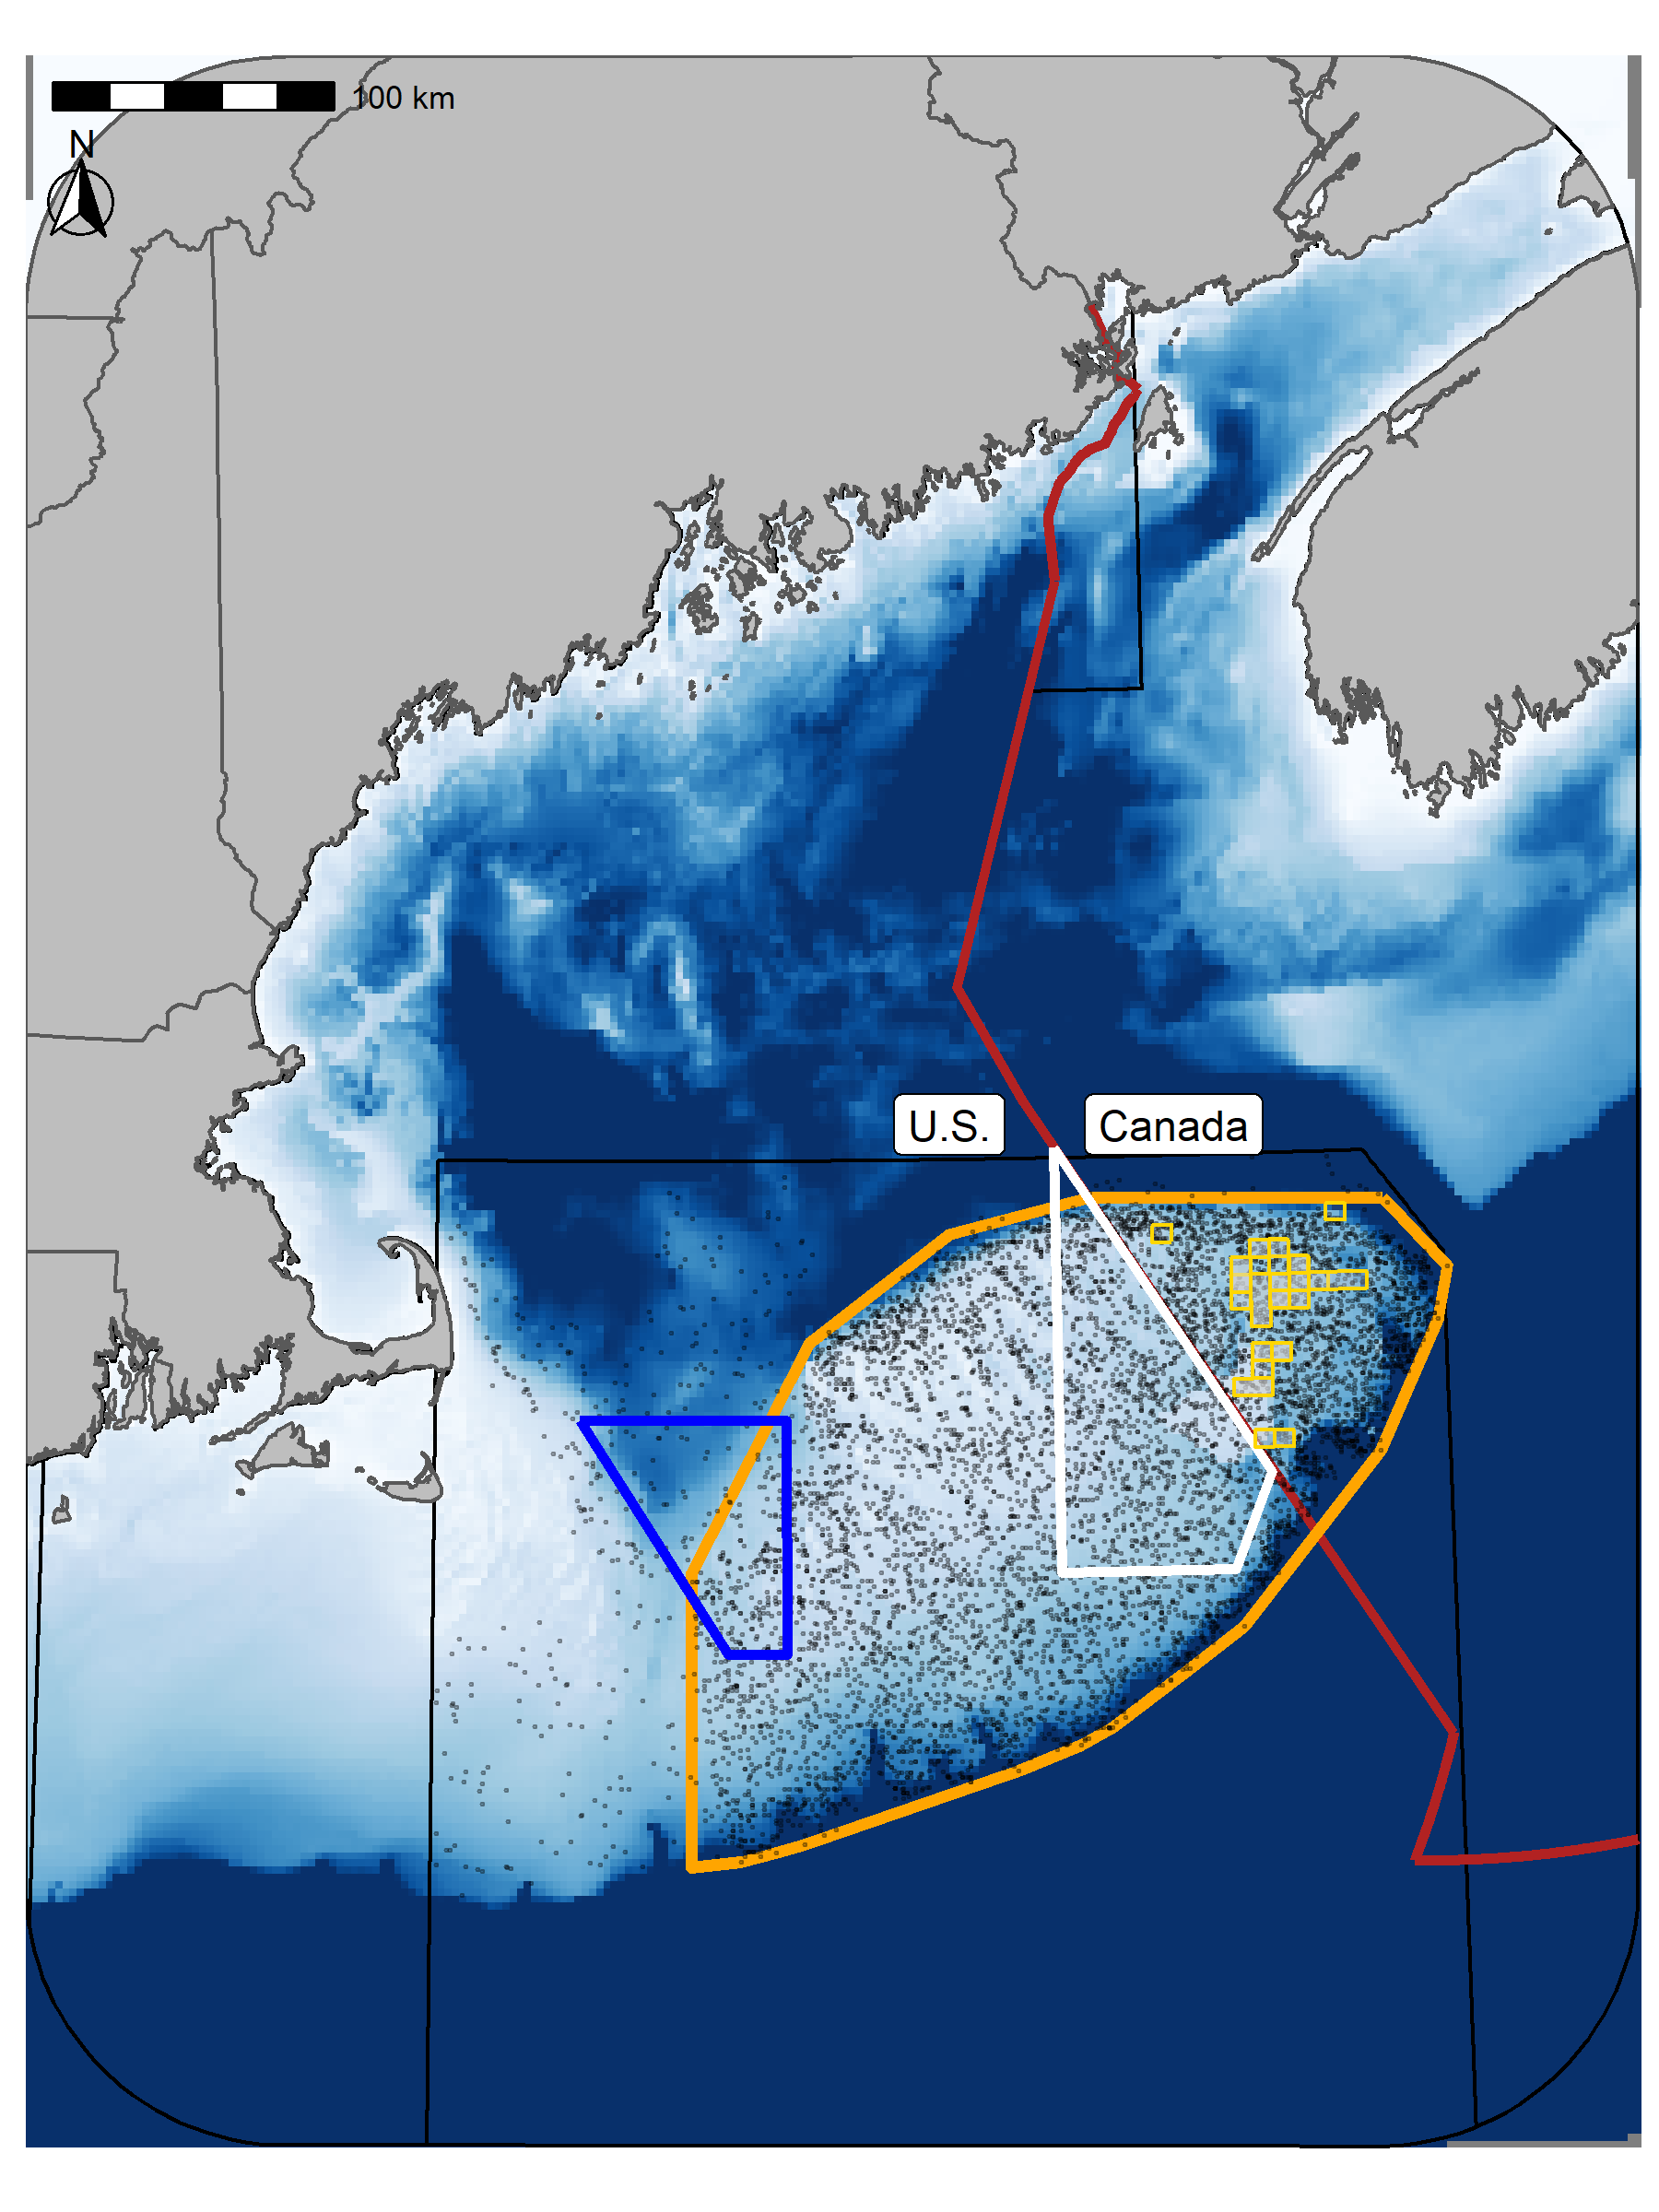
\includegraphics[width=1\linewidth]{D:/Github/Paper_2_SDMs/Results/Figures/GB_overview} 

}

\caption{Georges Bank (GB) study area.  Points represent the sample locations for each of the three surveys and the orange outline represets the core region of GB included in these analyses (42,000 km²).  The red line indicates the Canadian exclusive economic zone (EEZ).}\label{fig:Overview}
\end{figure}

\clearpage
\begin{figure}[htb]

{\centering 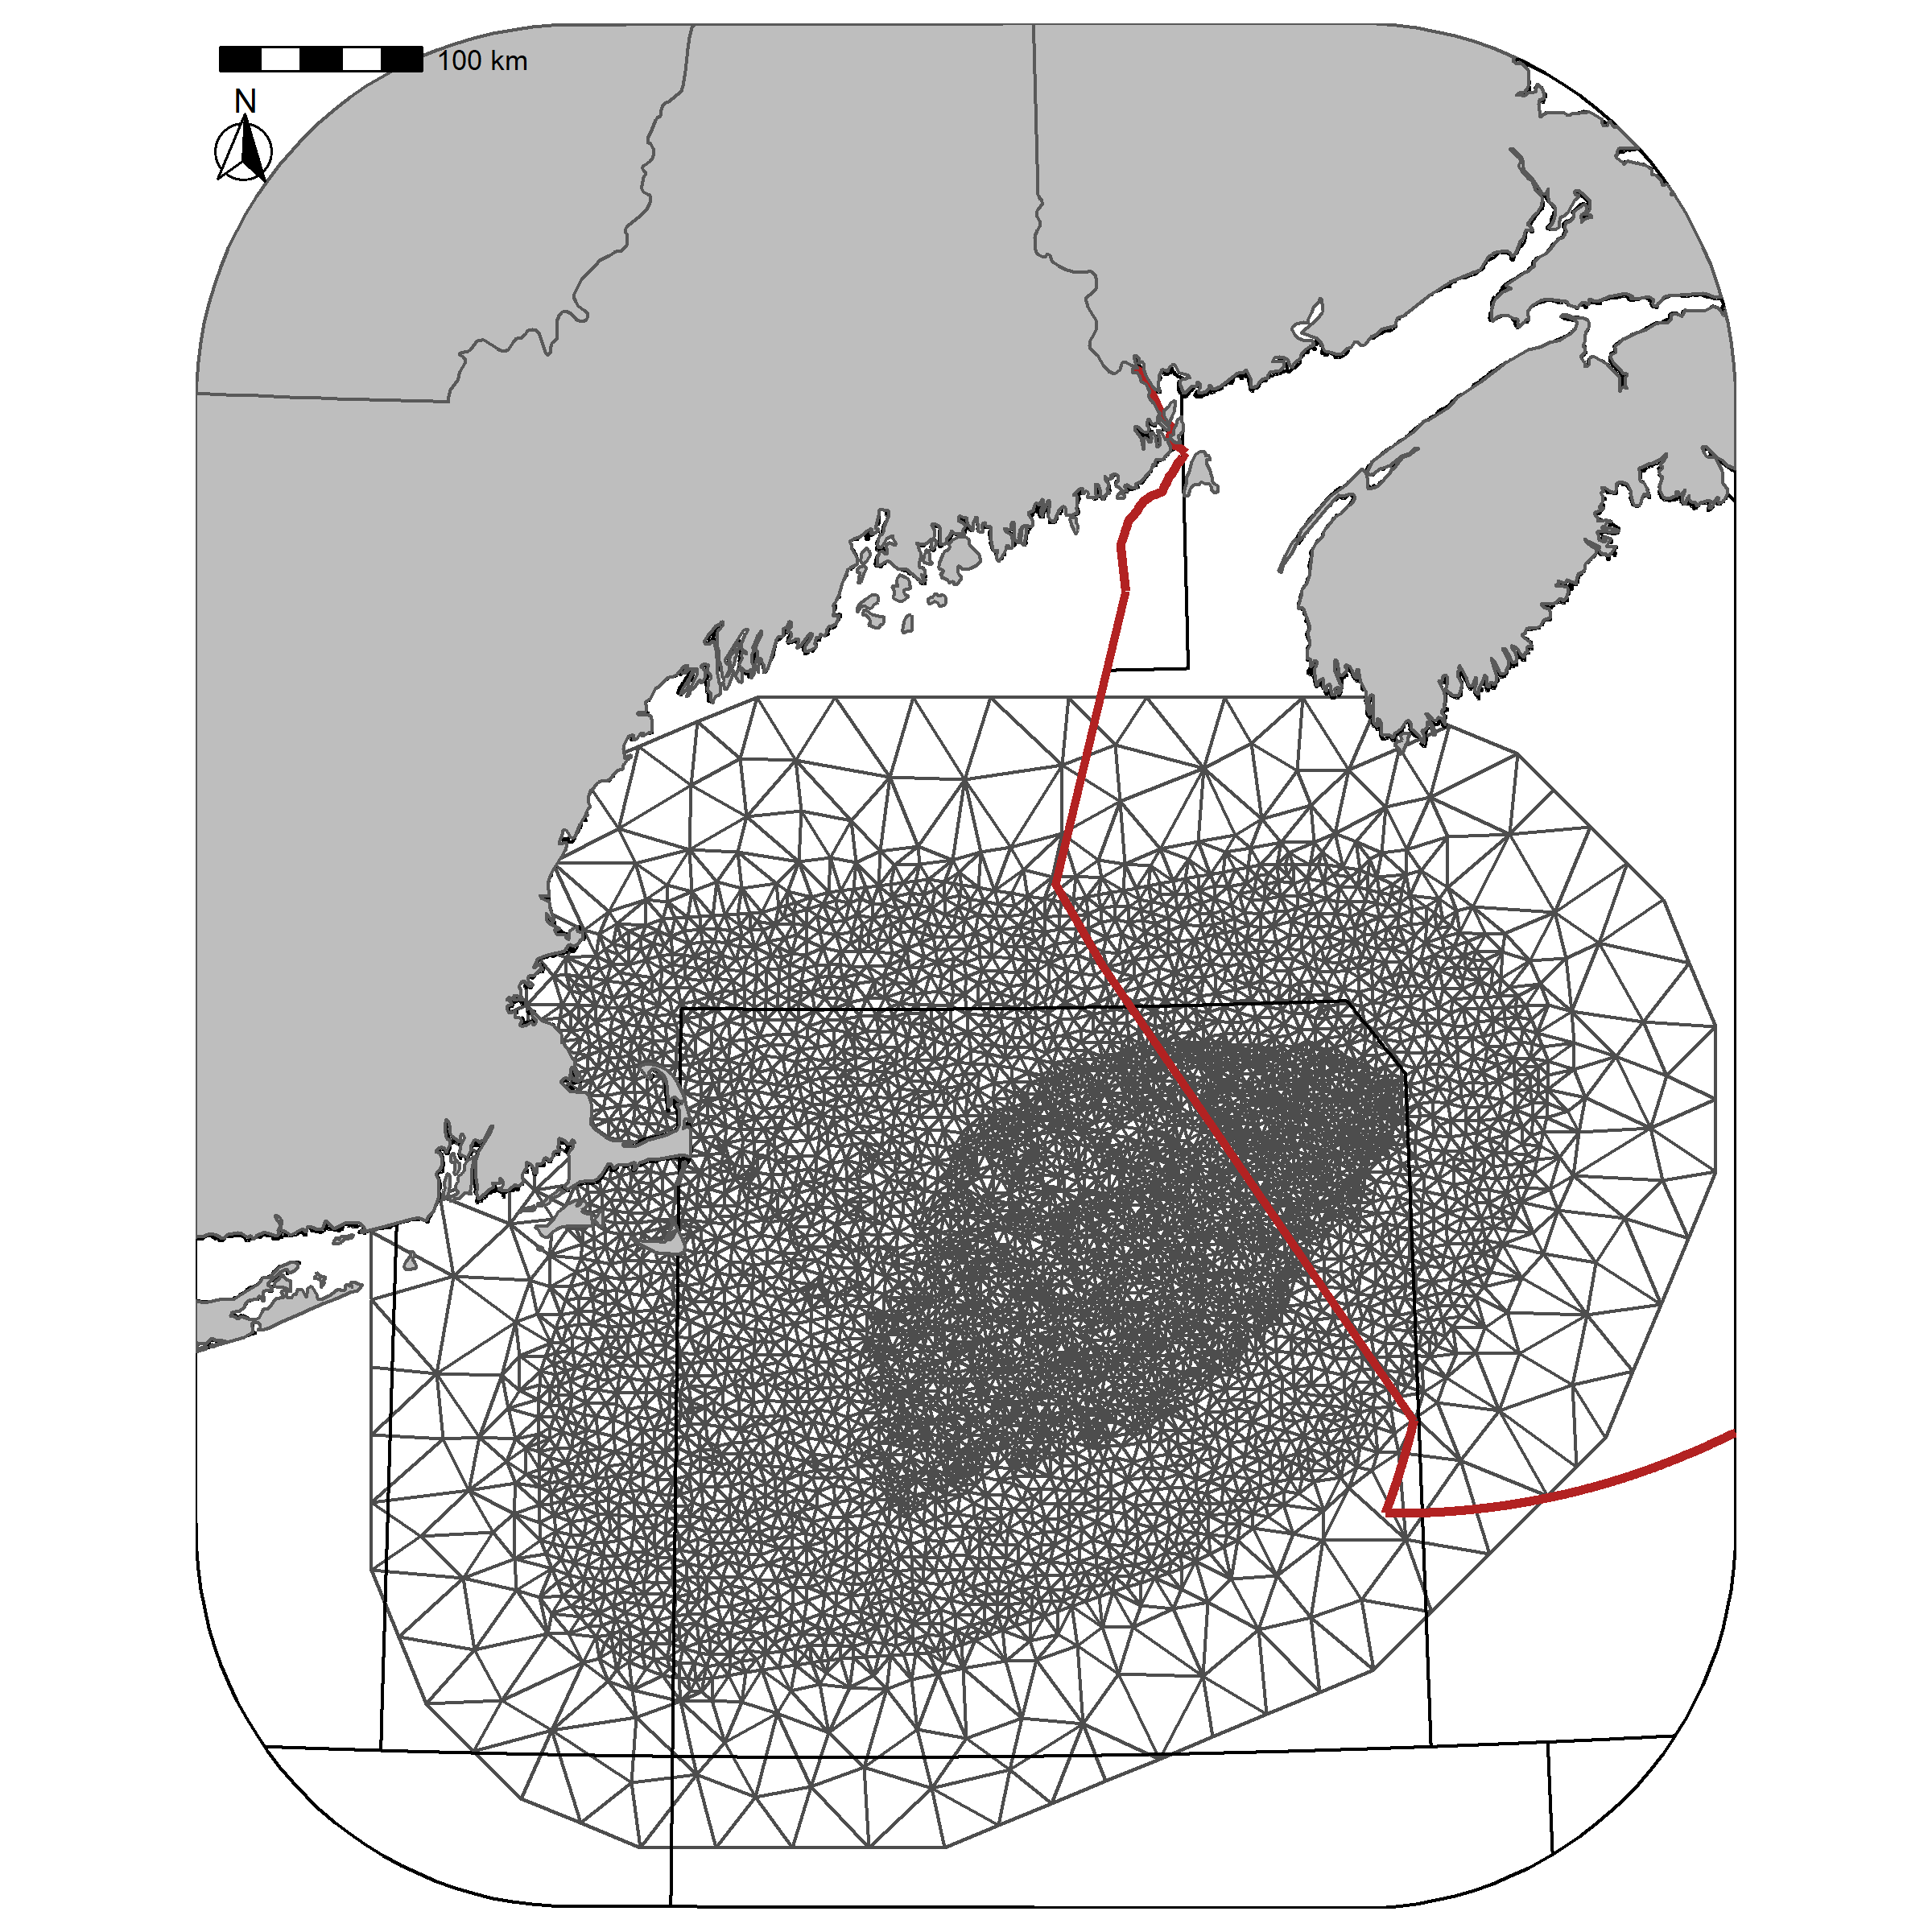
\includegraphics[width=1\linewidth]{D:/Github/Paper_2_SDMs/Results/Figures/mesh} 

}

\caption{Delaunay triangular mesh used for the spatial fields mesh. The mesh contains 6610 vertices.}\label{fig:Mesh}
\end{figure}

\begin{landscape}
\newpage
\begin{figure}[htb]

{\centering 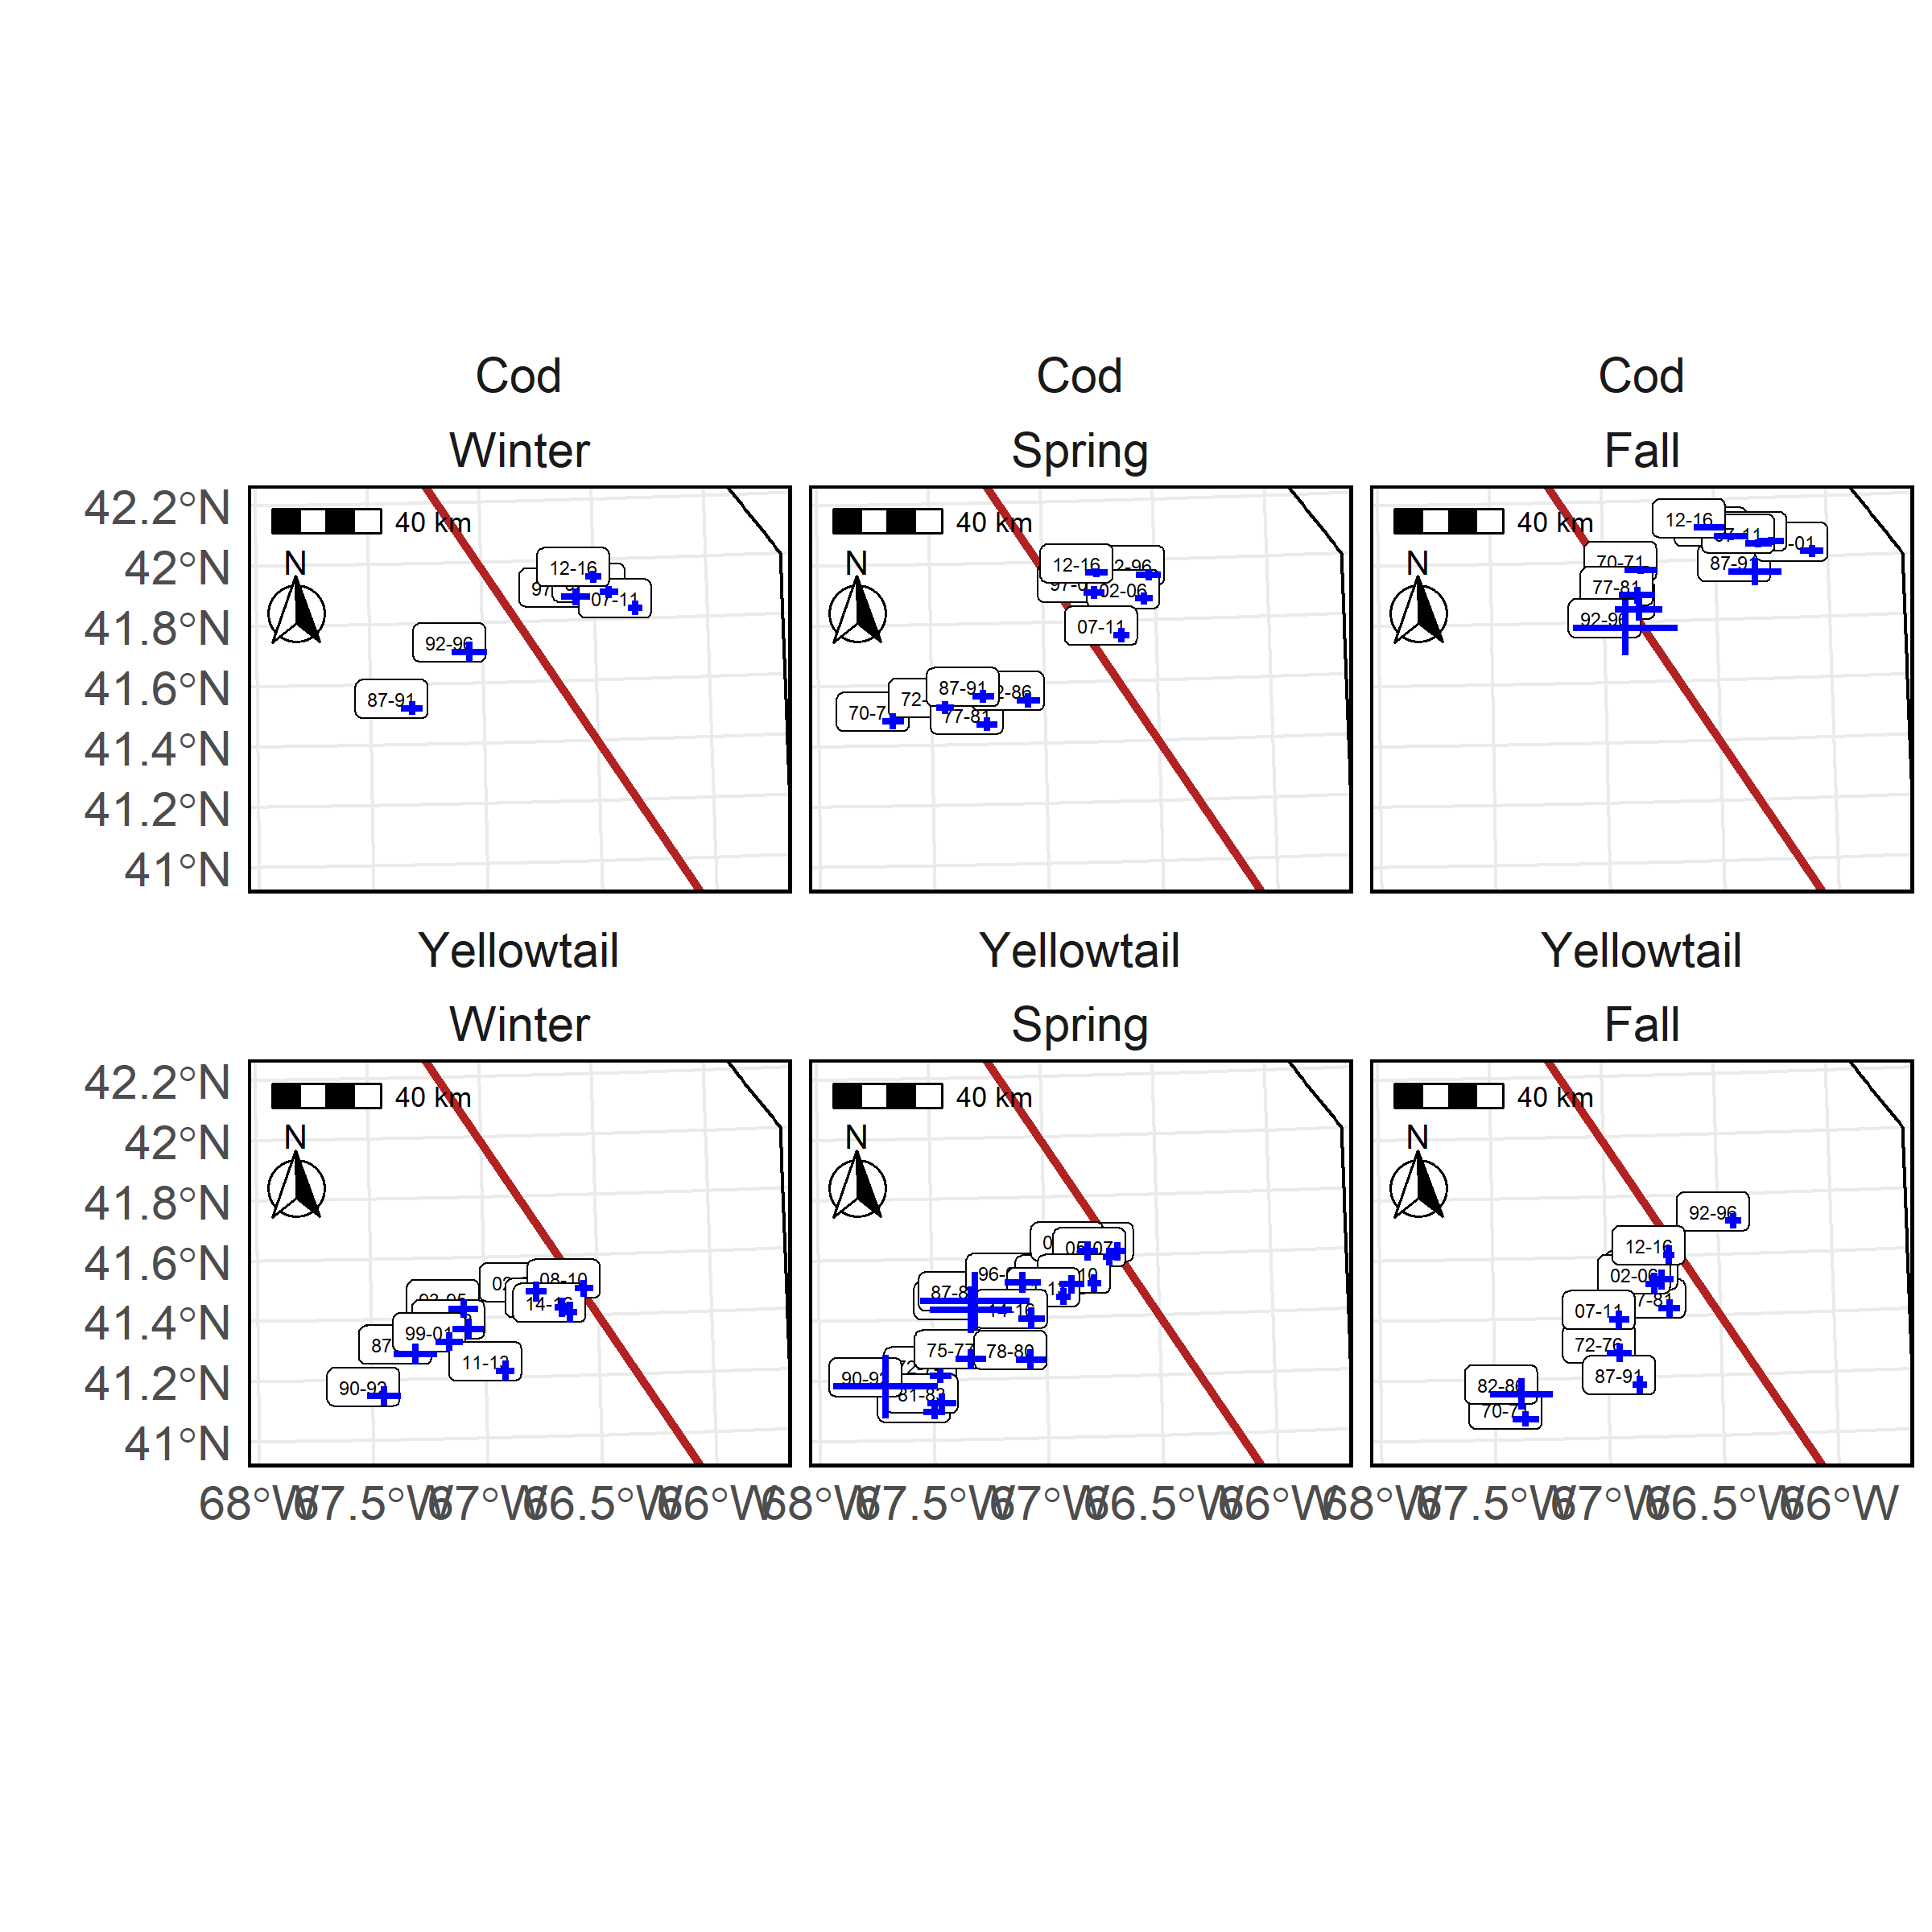
\includegraphics[width=1\linewidth]{D:/Github/Paper_2_SDMs/Results/Figures/center_of_gravity} 

}

\caption{Center of Gravity (COG) for the high EP areas for cod (top panel) and yellowtail (bottom panels) in the Winter (left), Spring (center), and Fall (right) using the preferred models.  Blue lines indicate ±3 standard deviation units from the mean COG. Labels indicate the years associated with each era and the red line is border between the U.S. and Canada.}\label{fig:cog-hep}
\end{figure}

\newpage
\begin{figure}[htb]

{\centering 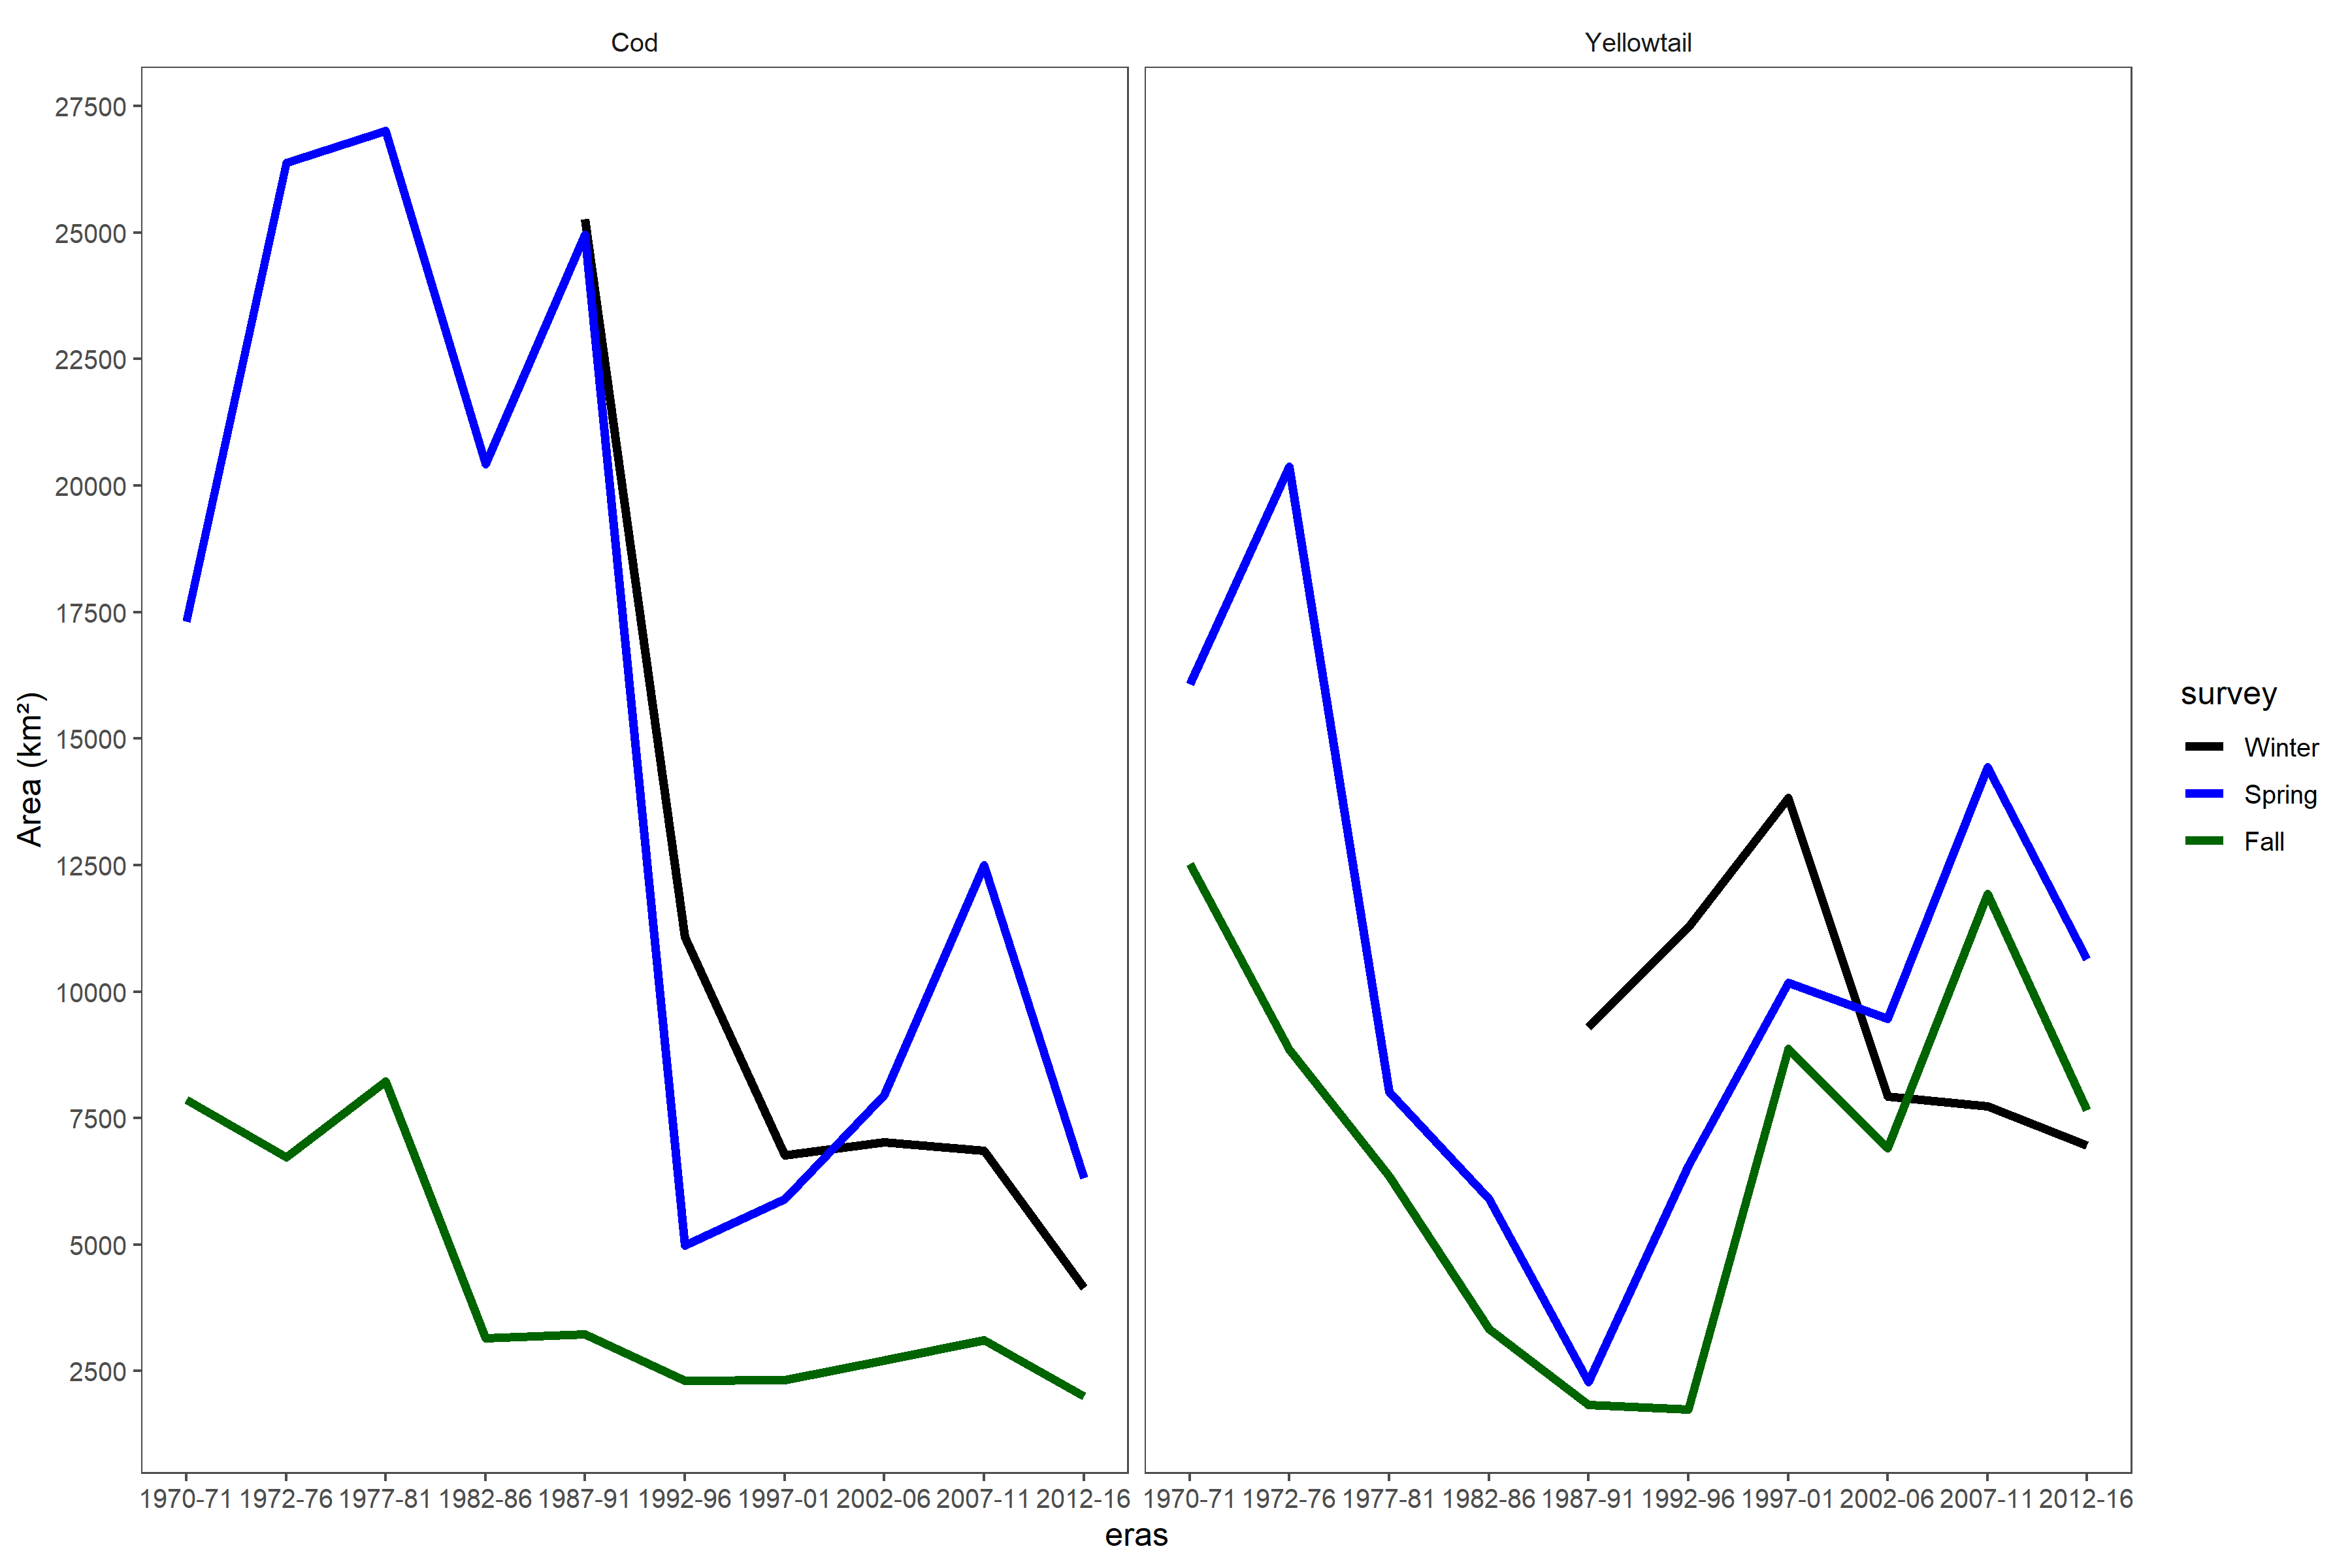
\includegraphics[width=1\linewidth]{D:/Github/Paper_2_SDMs/Results/Figures/Area_ts_high} 

}

\caption{Time series of the total area on GB classified as high EP for each of the three surveys using the preferred models.  The cod time series is on the left and the yellowtail on the right.  The black line represents the Winter trend, the Blue line is the Spring trend and the red line is the Fall trend.  }\label{fig:area-hep}
\end{figure}

\newpage
\begin{figure}[htb]

{\centering 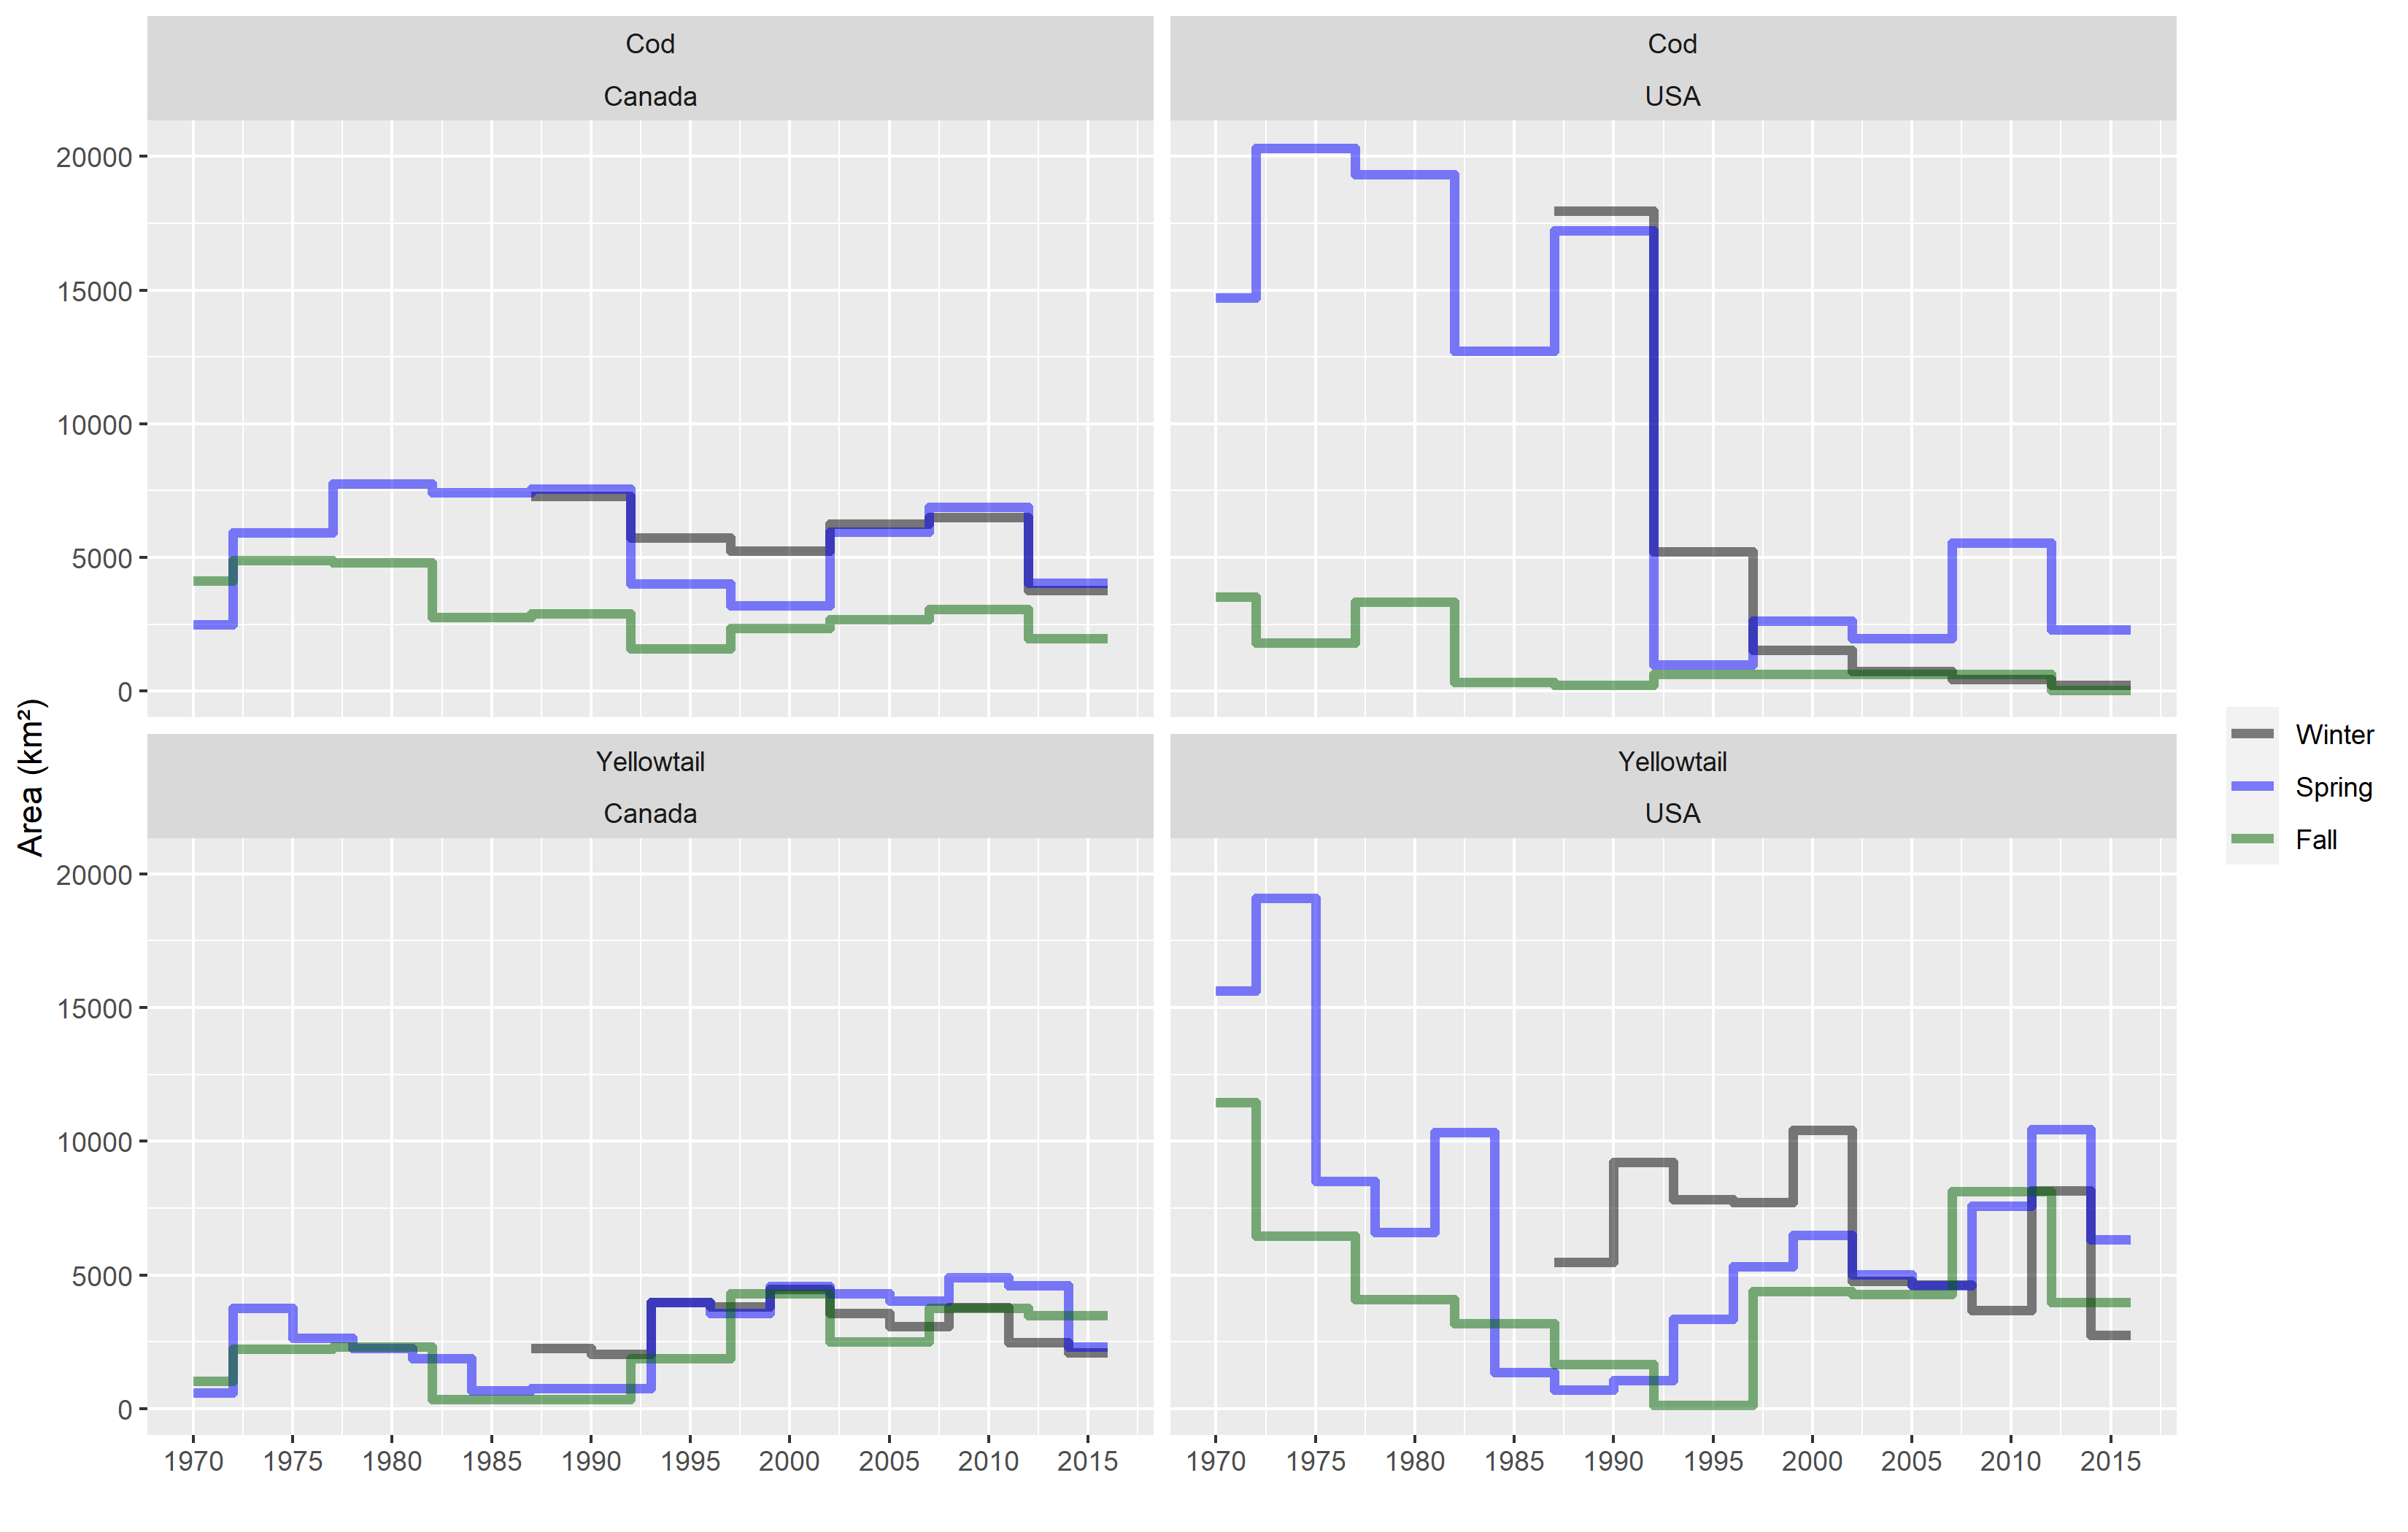
\includegraphics[width=1\linewidth]{D:/Github/Paper_2_SDMs/Results/Figures/Area_can_vs_us_ts_high} 

}

\caption{Time series of the total area on GB classified as core area for each of the three seasons in Canada and the U.S..  The Atlantic Cod time series is in the top row and Yellowtail Flounder in the bottom row, Canada is on the left and U.S. is on the right.  The black line represents the Winter trend, the Blue line is the Spring trend and the green line is the Fall trend.  }\label{fig:area-can-vs-us-hep}
\end{figure}

\newpage
\begin{figure}[htb]

{\centering 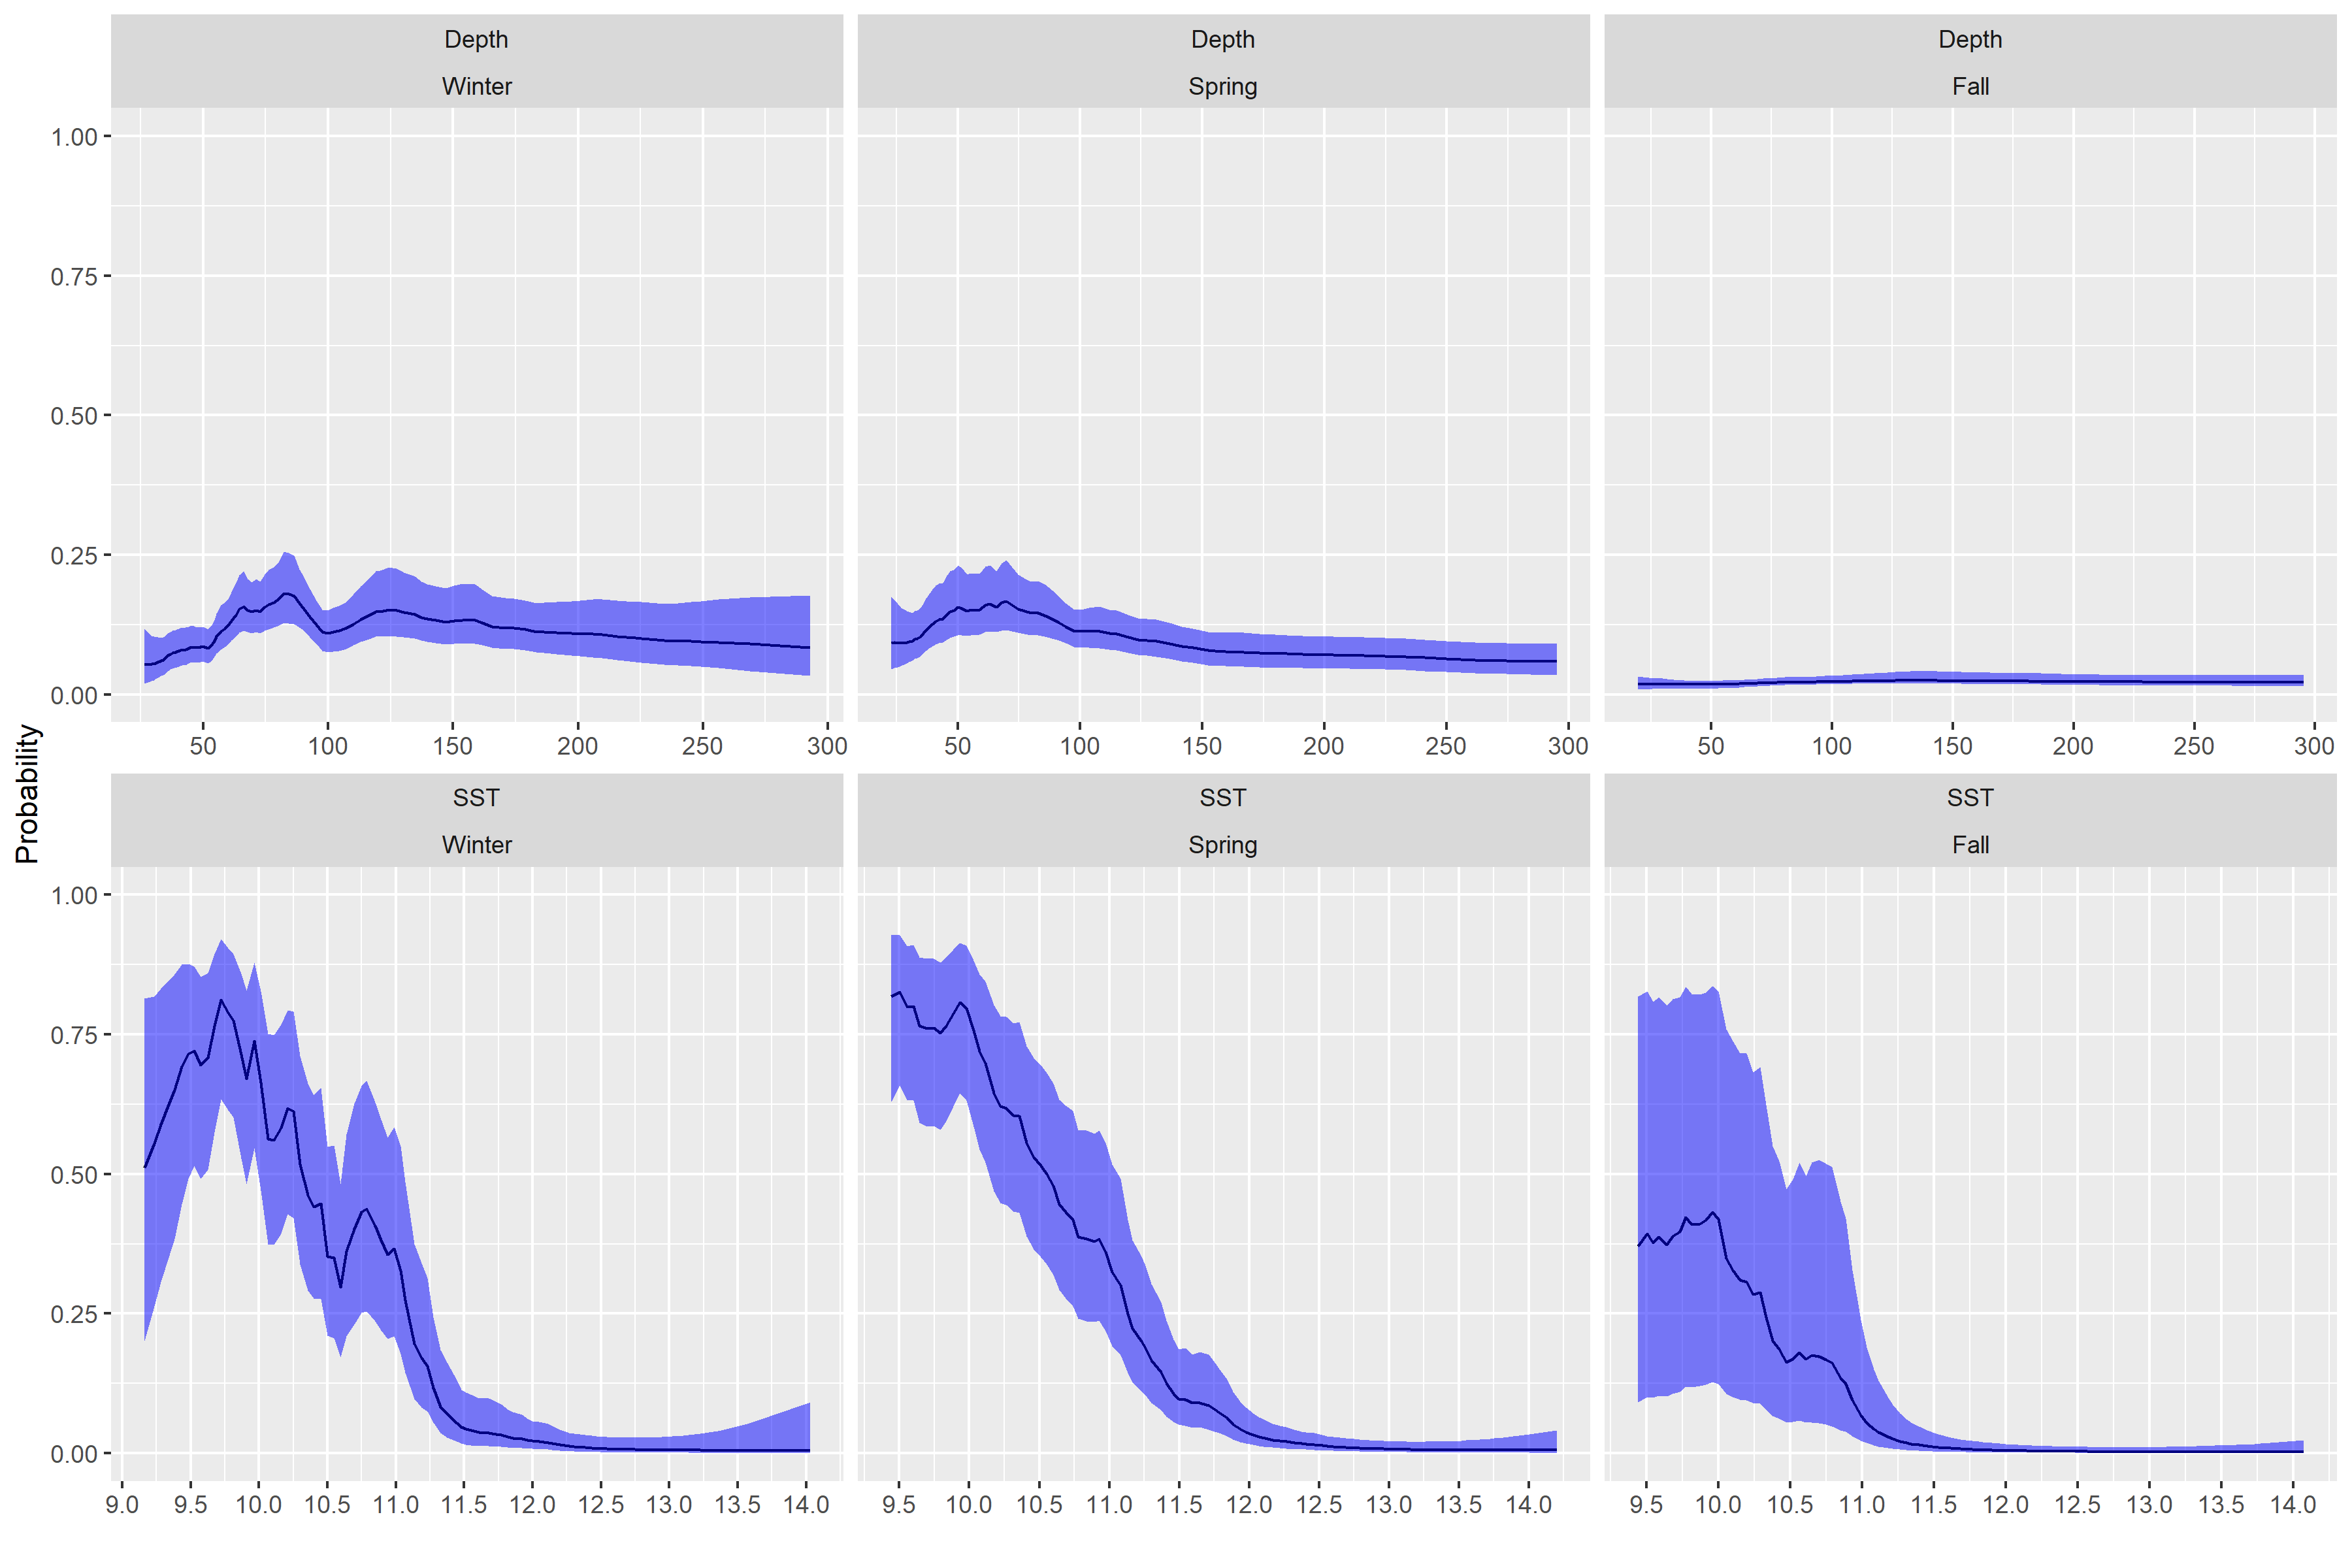
\includegraphics[width=1\linewidth]{D:/Github/Paper_2_SDMs/Results/Figures/Cod_fixed_effects} 

}

\caption{Fixed effects for cod from each survey, top row is the depth covariate effect, bottom row is the SST effect. Results transformed to the probability scale and the blue shaded region represents the 95\% credible interval.}\label{fig:cod-fe}
\end{figure}

\newpage
\begin{figure}[htb]

{\centering 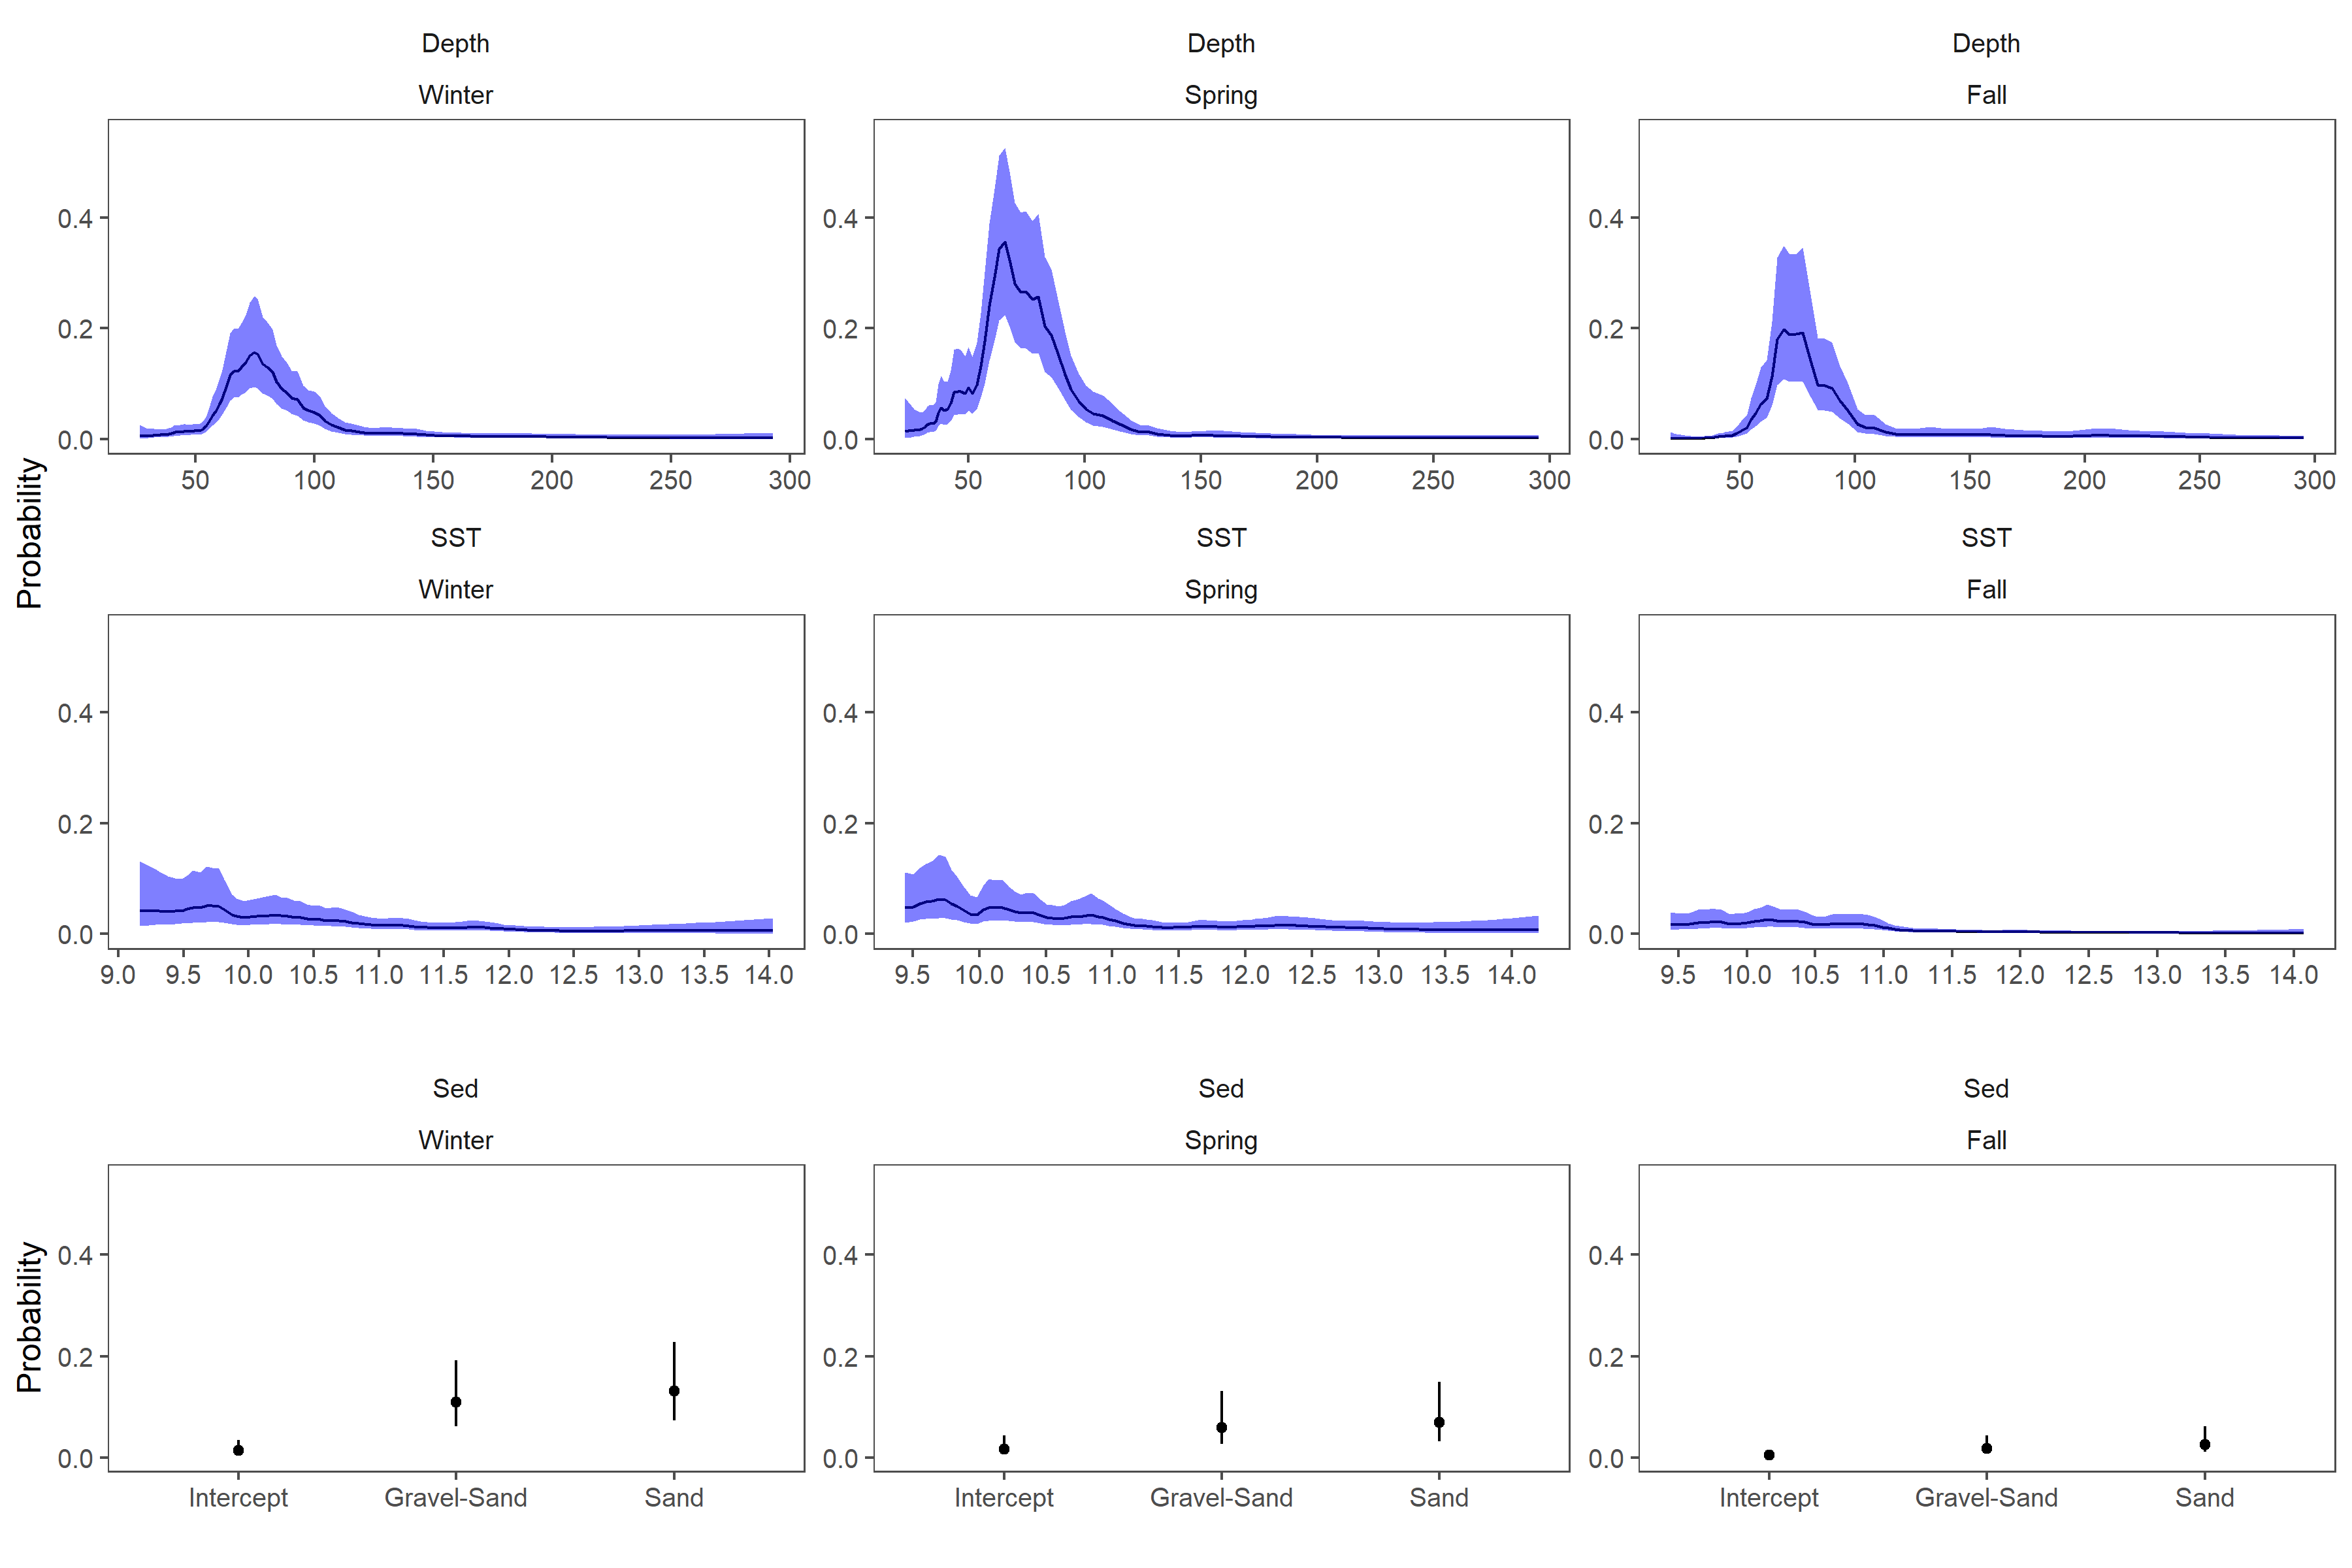
\includegraphics[width=1\linewidth]{D:/Github/Paper_2_SDMs/Results/Figures/yt_fixed_effects} 

}

\caption{Fixed effects for yellowtail from each survey, the top row is the depth covariate effect, middle row is the SST effect and the bottom row is the effect of sediment type. Results transformed to the probability scale, and the blue shaded region and the error bars represent the 95\% credible intervals. The winter and spring results use a 3 year random field while the fall results are for the preferred 5 year random field model.}\label{fig:yt-fe}
\end{figure}

\clearpage

\begin{figure}[htb]

{\centering \includegraphics[width=1\linewidth]{D:/Github/Paper_2_SDMs/Results/Figures/hyper_range_field_est} 

}

\caption{Decorrelation range estimate with 95\%CI's for each season.}\label{fig:hyper-range-var-est}
\end{figure}

\clearpage

\begin{figure}[htb]

{\centering \includegraphics[width=1\linewidth]{D:/Github/Paper_2_SDMs/Results/Figures/hyper_sd_field_est} 

}

\caption{Standard Deviation of the field with 95\%CI's for each season.}\label{fig:hyper-sd-var-est}
\end{figure}

\newpage
\begin{figure}[htb]

{\centering 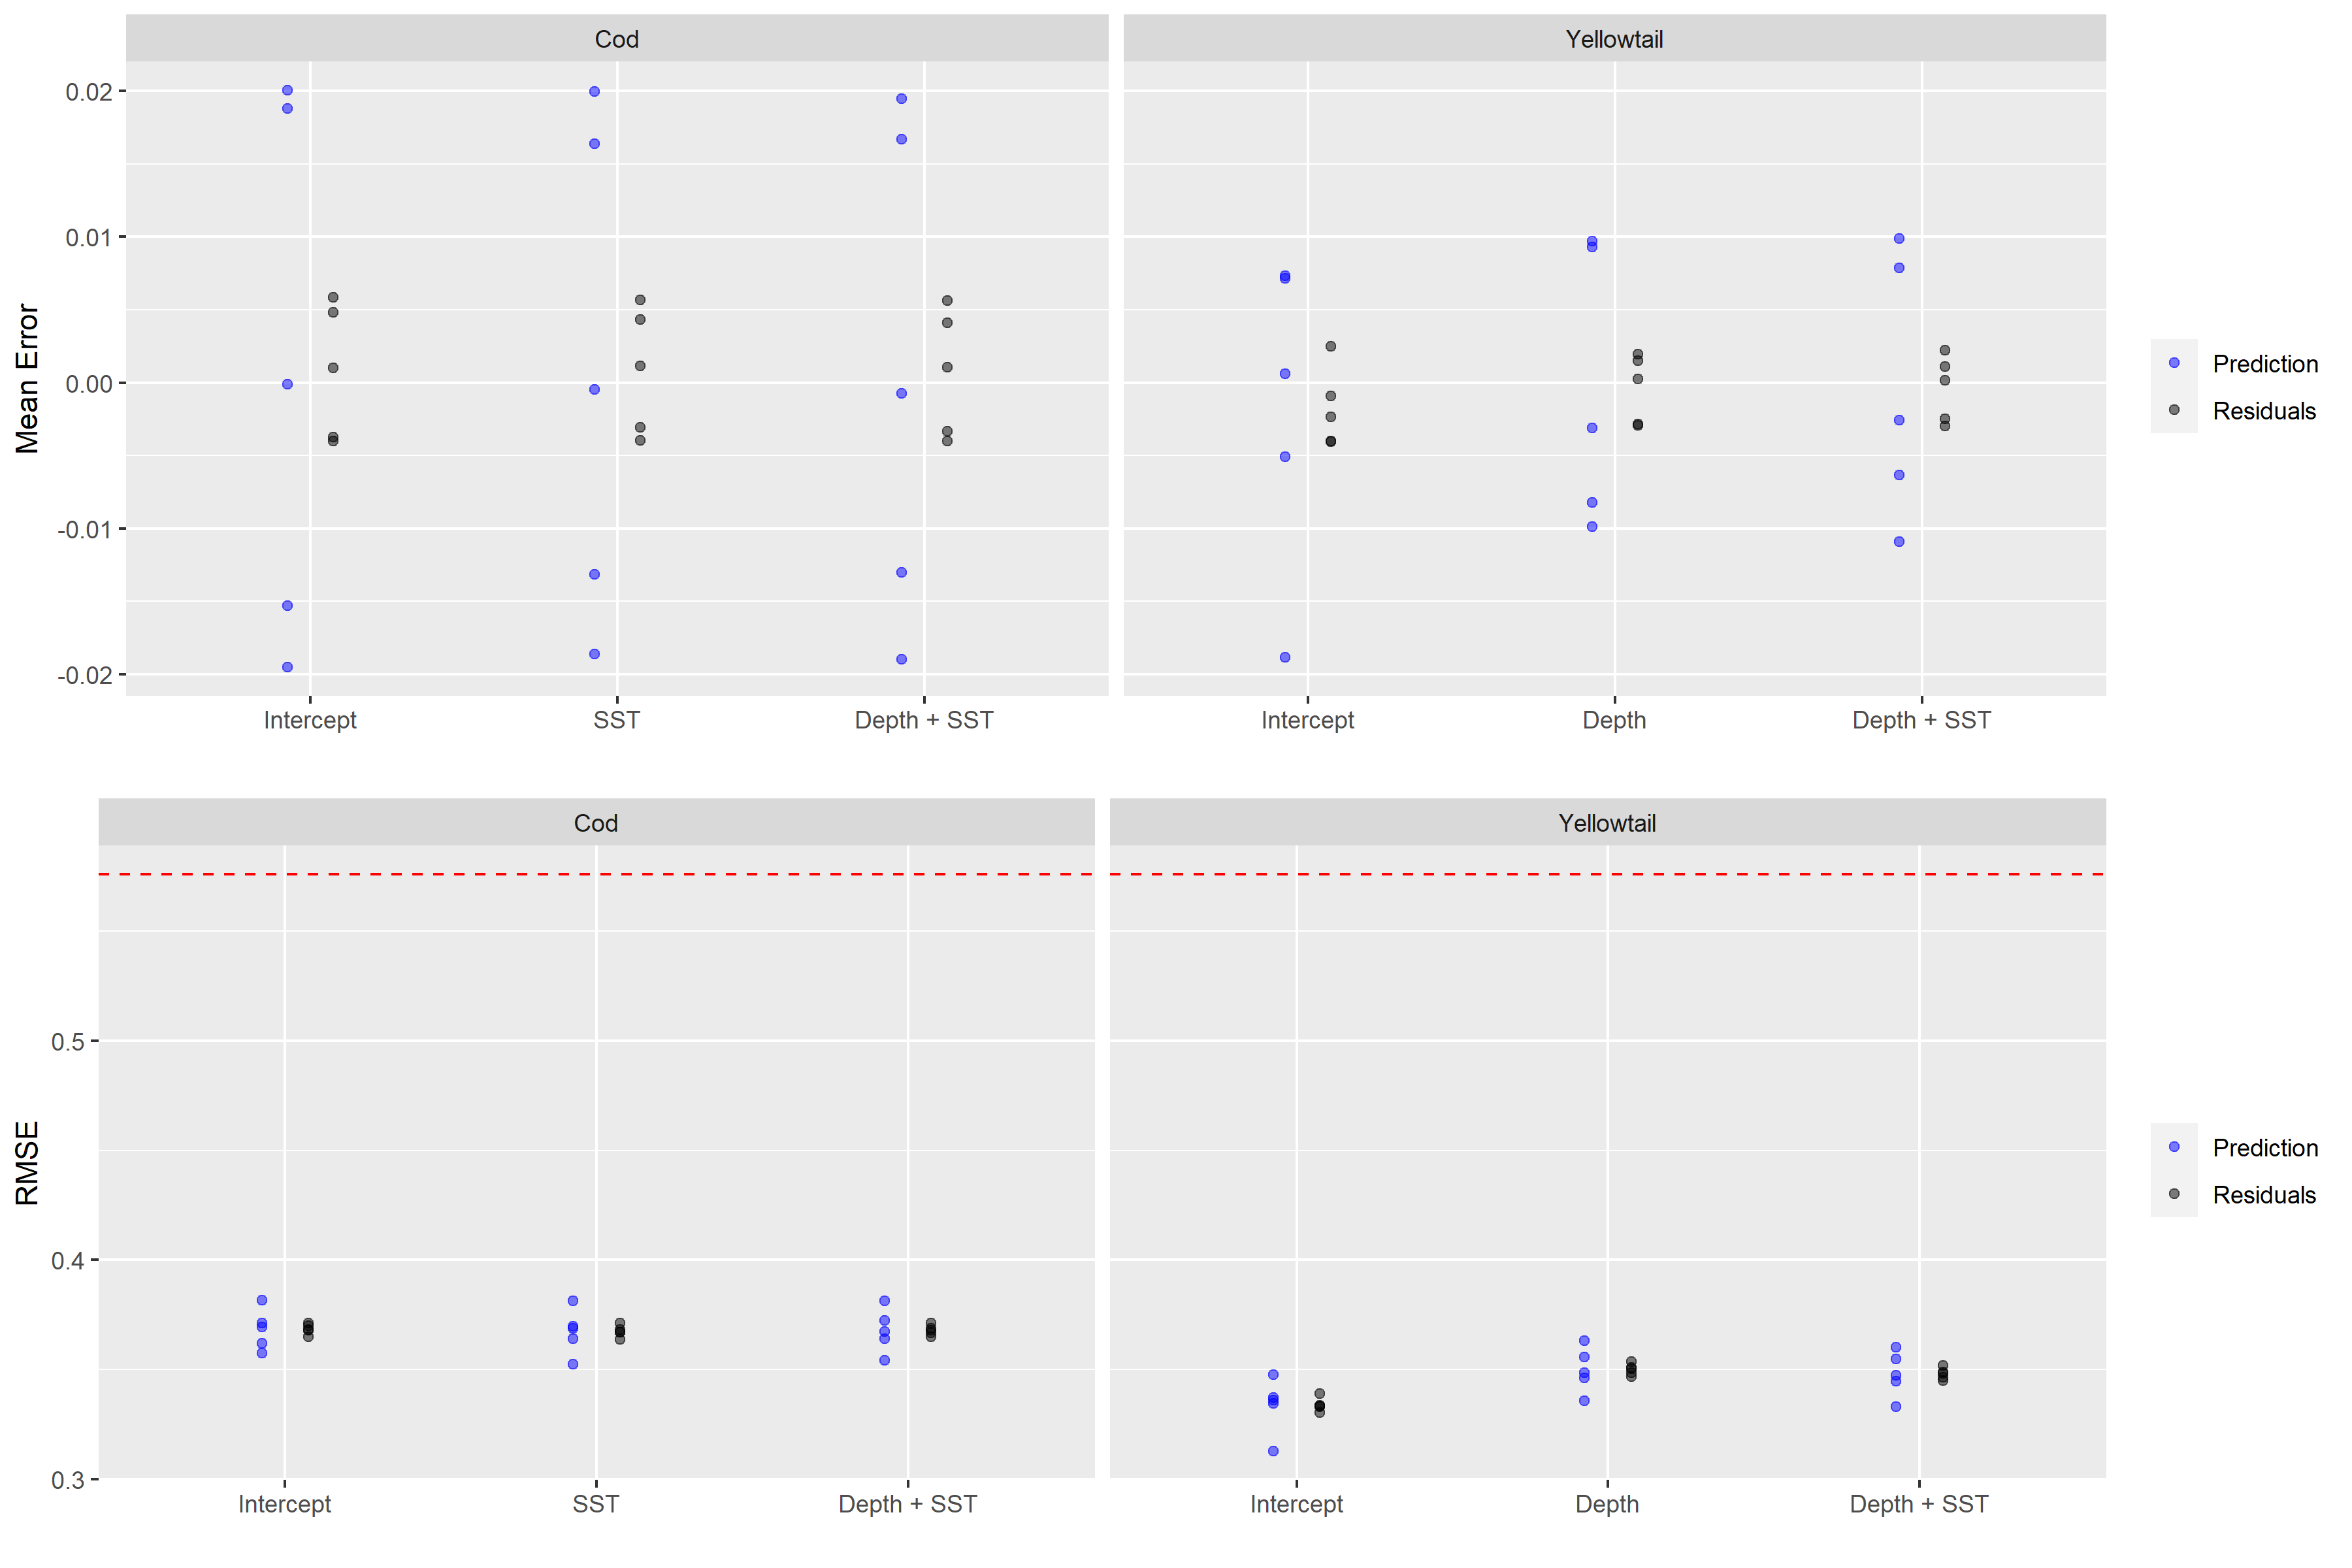
\includegraphics[width=1\linewidth]{D:/Github/Paper_2_SDMs/Results/Figures/cross_fold_validation} 

}

\caption{Results of 5 fold cross validation analyses. Top panels represents the mean error for each of the three covariate models tested for cod and yellowtail. Blue points represent the prediction error from the testing dataset, while the black points are the residuals from the training dataset. The bottom panels are the Root Mean Squared Error (RMSE) for these models.  The dashed line represents the RMSE for randomly generated data and represents the RMSE for a model with no predictive ability. All models use the 5 year random field due to computational constraints.}\label{fig:folds}
\end{figure}

\newpage
\begin{figure}[htb]

{\centering 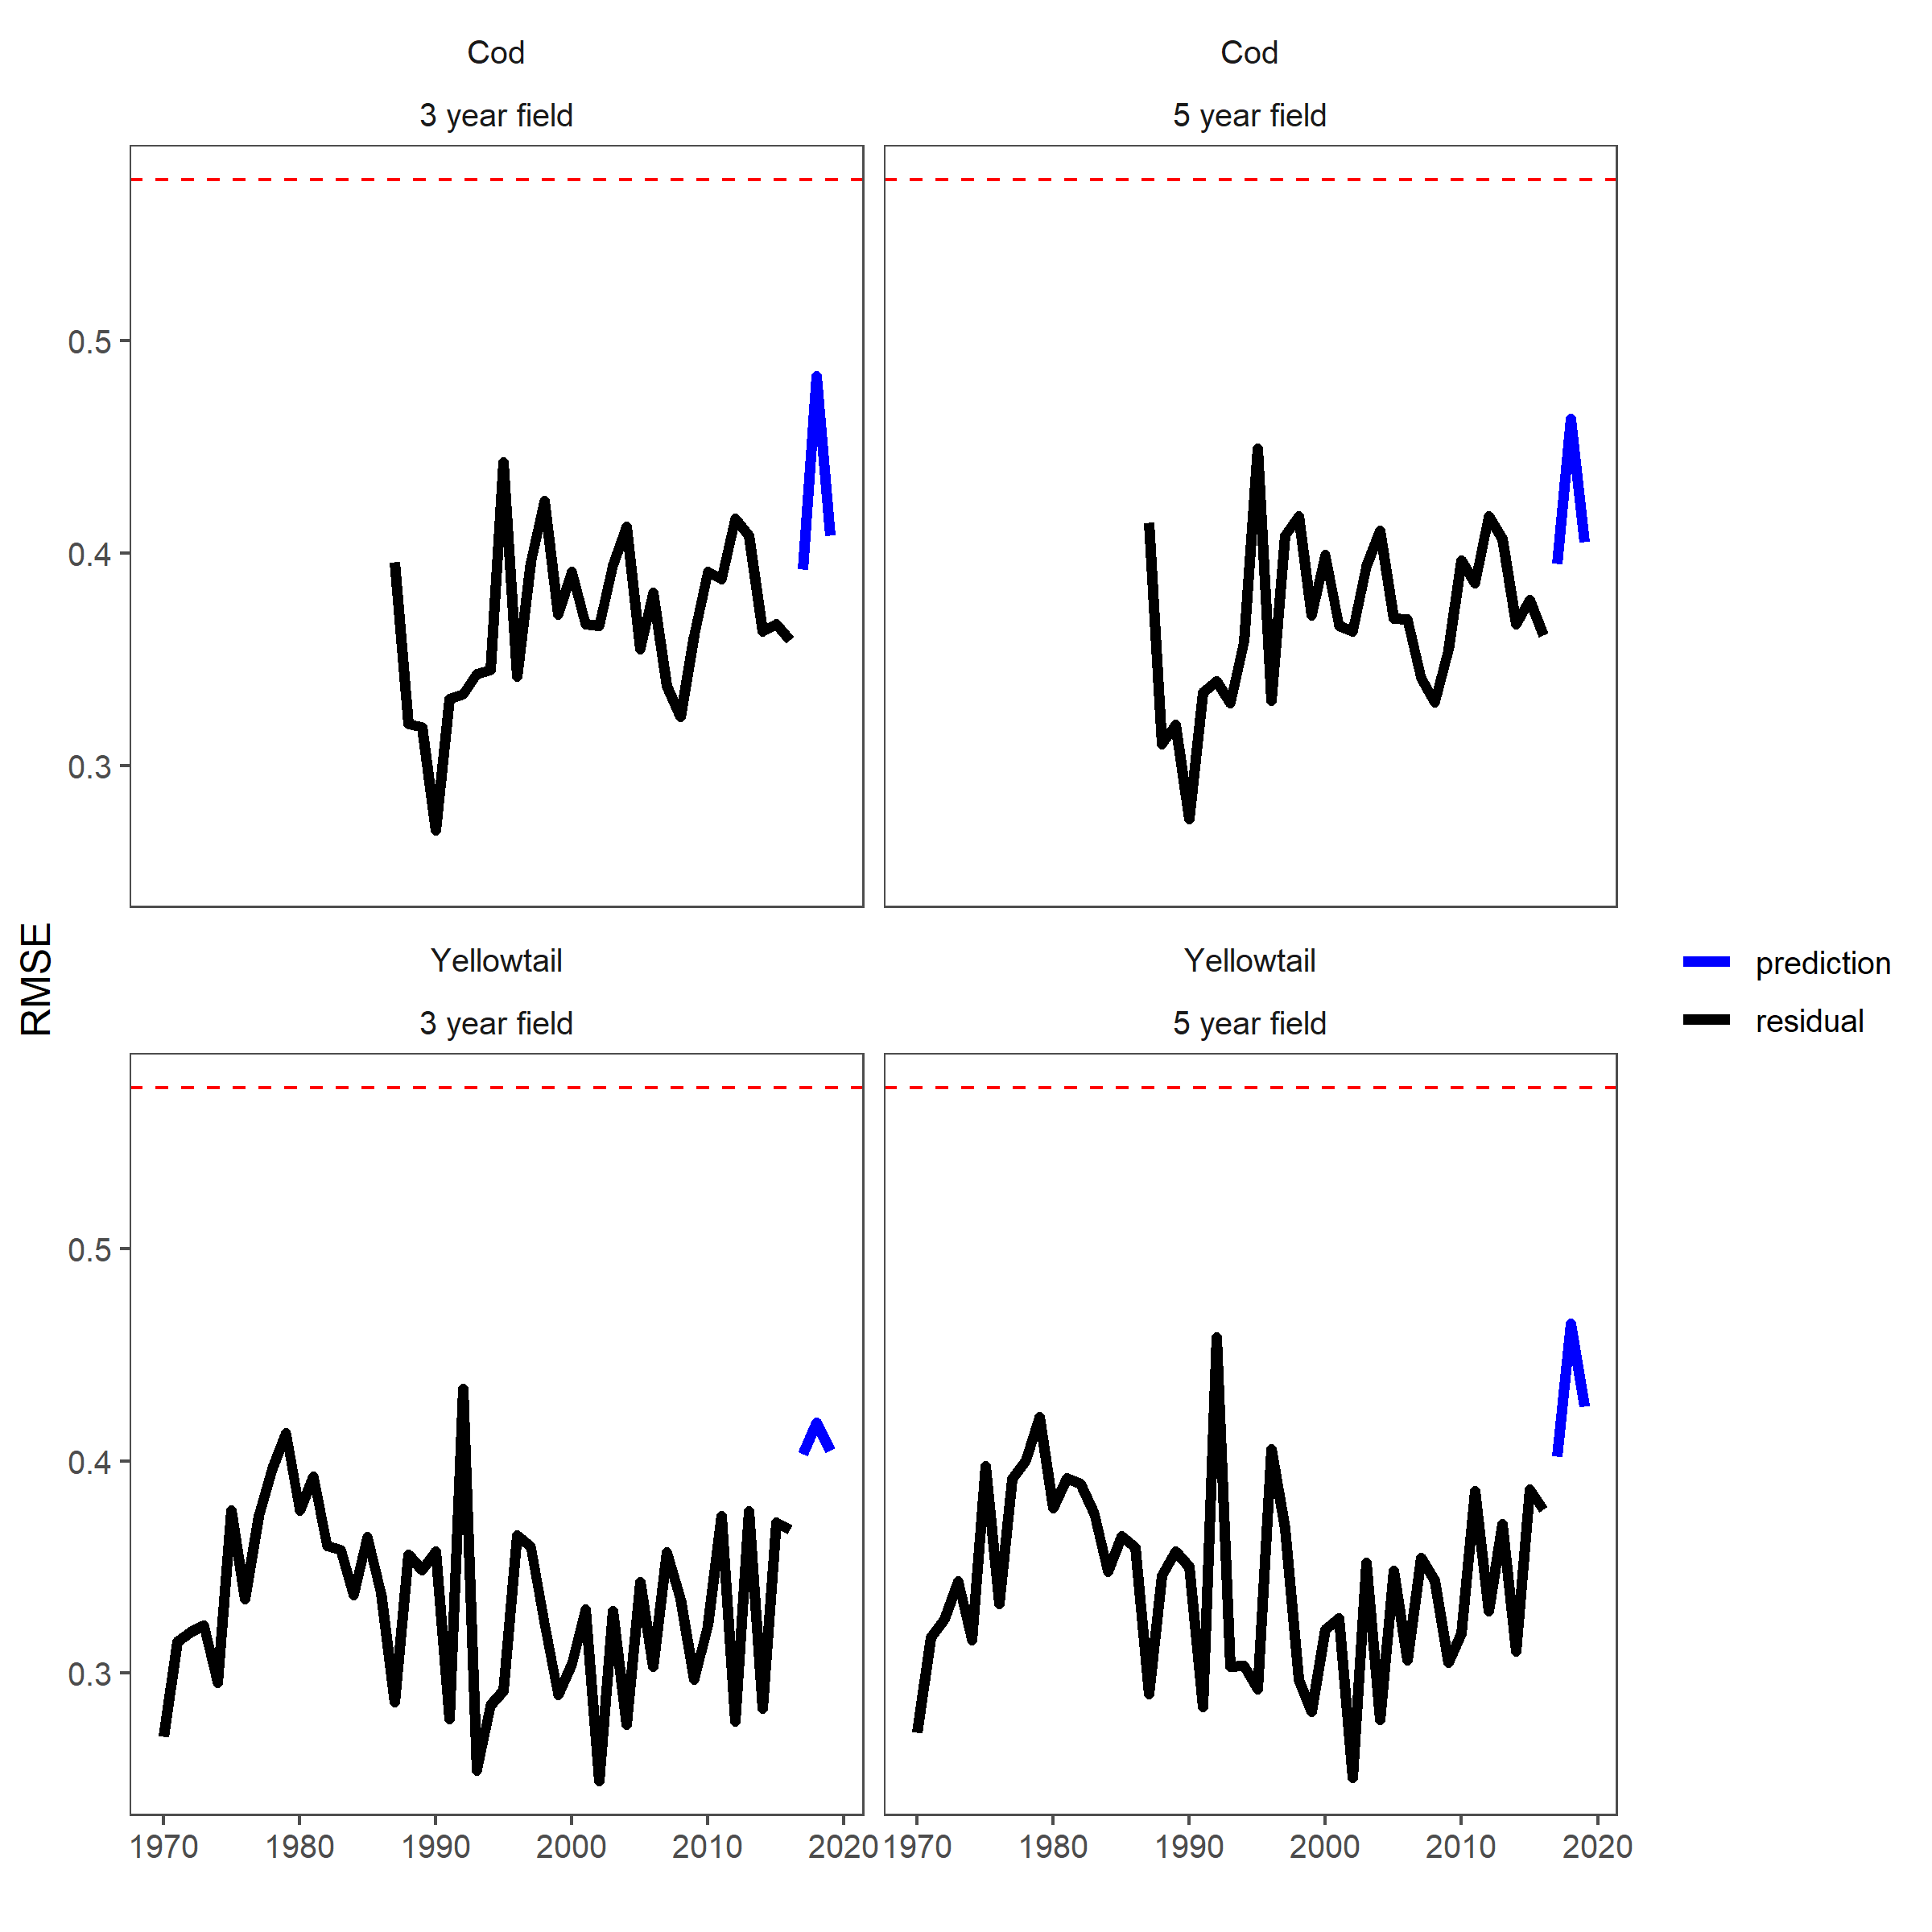
\includegraphics[width=1\linewidth]{D:/Github/Paper_2_SDMs/Results/Figures/prediction_2017_2019} 

}

\caption{The residual Root Mean Squared Error for the model is shown in black, while the blue lines represent the prediction RMSE for data in years 2017, 2018, and 2019. The models compared were a model with no covariates (intercept + random field) represented with a dashed line and a model which includes the additive SST and Depth covariates along with the random field represented with the solid line.  The cod results are in the top row and use a 5 year random field. The yellowtail results are in the bottom row and use a 3 year random field for the Winter and Spring andd the 5 year random field for the Fall. The red dot-dash line represents the RMSE for randomly generated data and represents the RMSE for a model with no predictive ability.}\label{fig:pred-17-19}
\end{figure}

\end{landscape}

\newpage

\hypertarget{ref-sup}{%
\section{SUPPLEMENT 1}\label{ref-sup}}

\setcounter{table}{0}  \renewcommand{\thetable}{S\arabic{table}} \setcounter{figure}{0} \renewcommand{\thefigure}{S\arabic{figure}}

\newpage
\begin{landscape}
\begin{figure}[htb]

{\centering \includegraphics[width=0.75\linewidth]{D:/Github/Paper_2_SDMs/Results/Figures/pca} 

}

\caption{Princpal Component Analysis (PCA) results for the Winter, Spring, and Fall seasons using the retained environmental data and the 4 retained Princpal Components (PCs). The results for PC 1 and 2 for each season are on the top and the PC 3 and 4 results are on the bottom.  Left column are the results for Winter, middle column for Spring, and right column is for the Fall. The percentage of the variance exaplained by each PC is provided on the axes labels.  Points represent the score for each survey observation.  The loadings for each covariate in the analysis are shown by the length of their respective lines. PC scores greater than ± 3 units not shown.}\label{fig:PCA}
\end{figure}

\newpage

\clearpage
\begin{figure}[htb]

{\centering 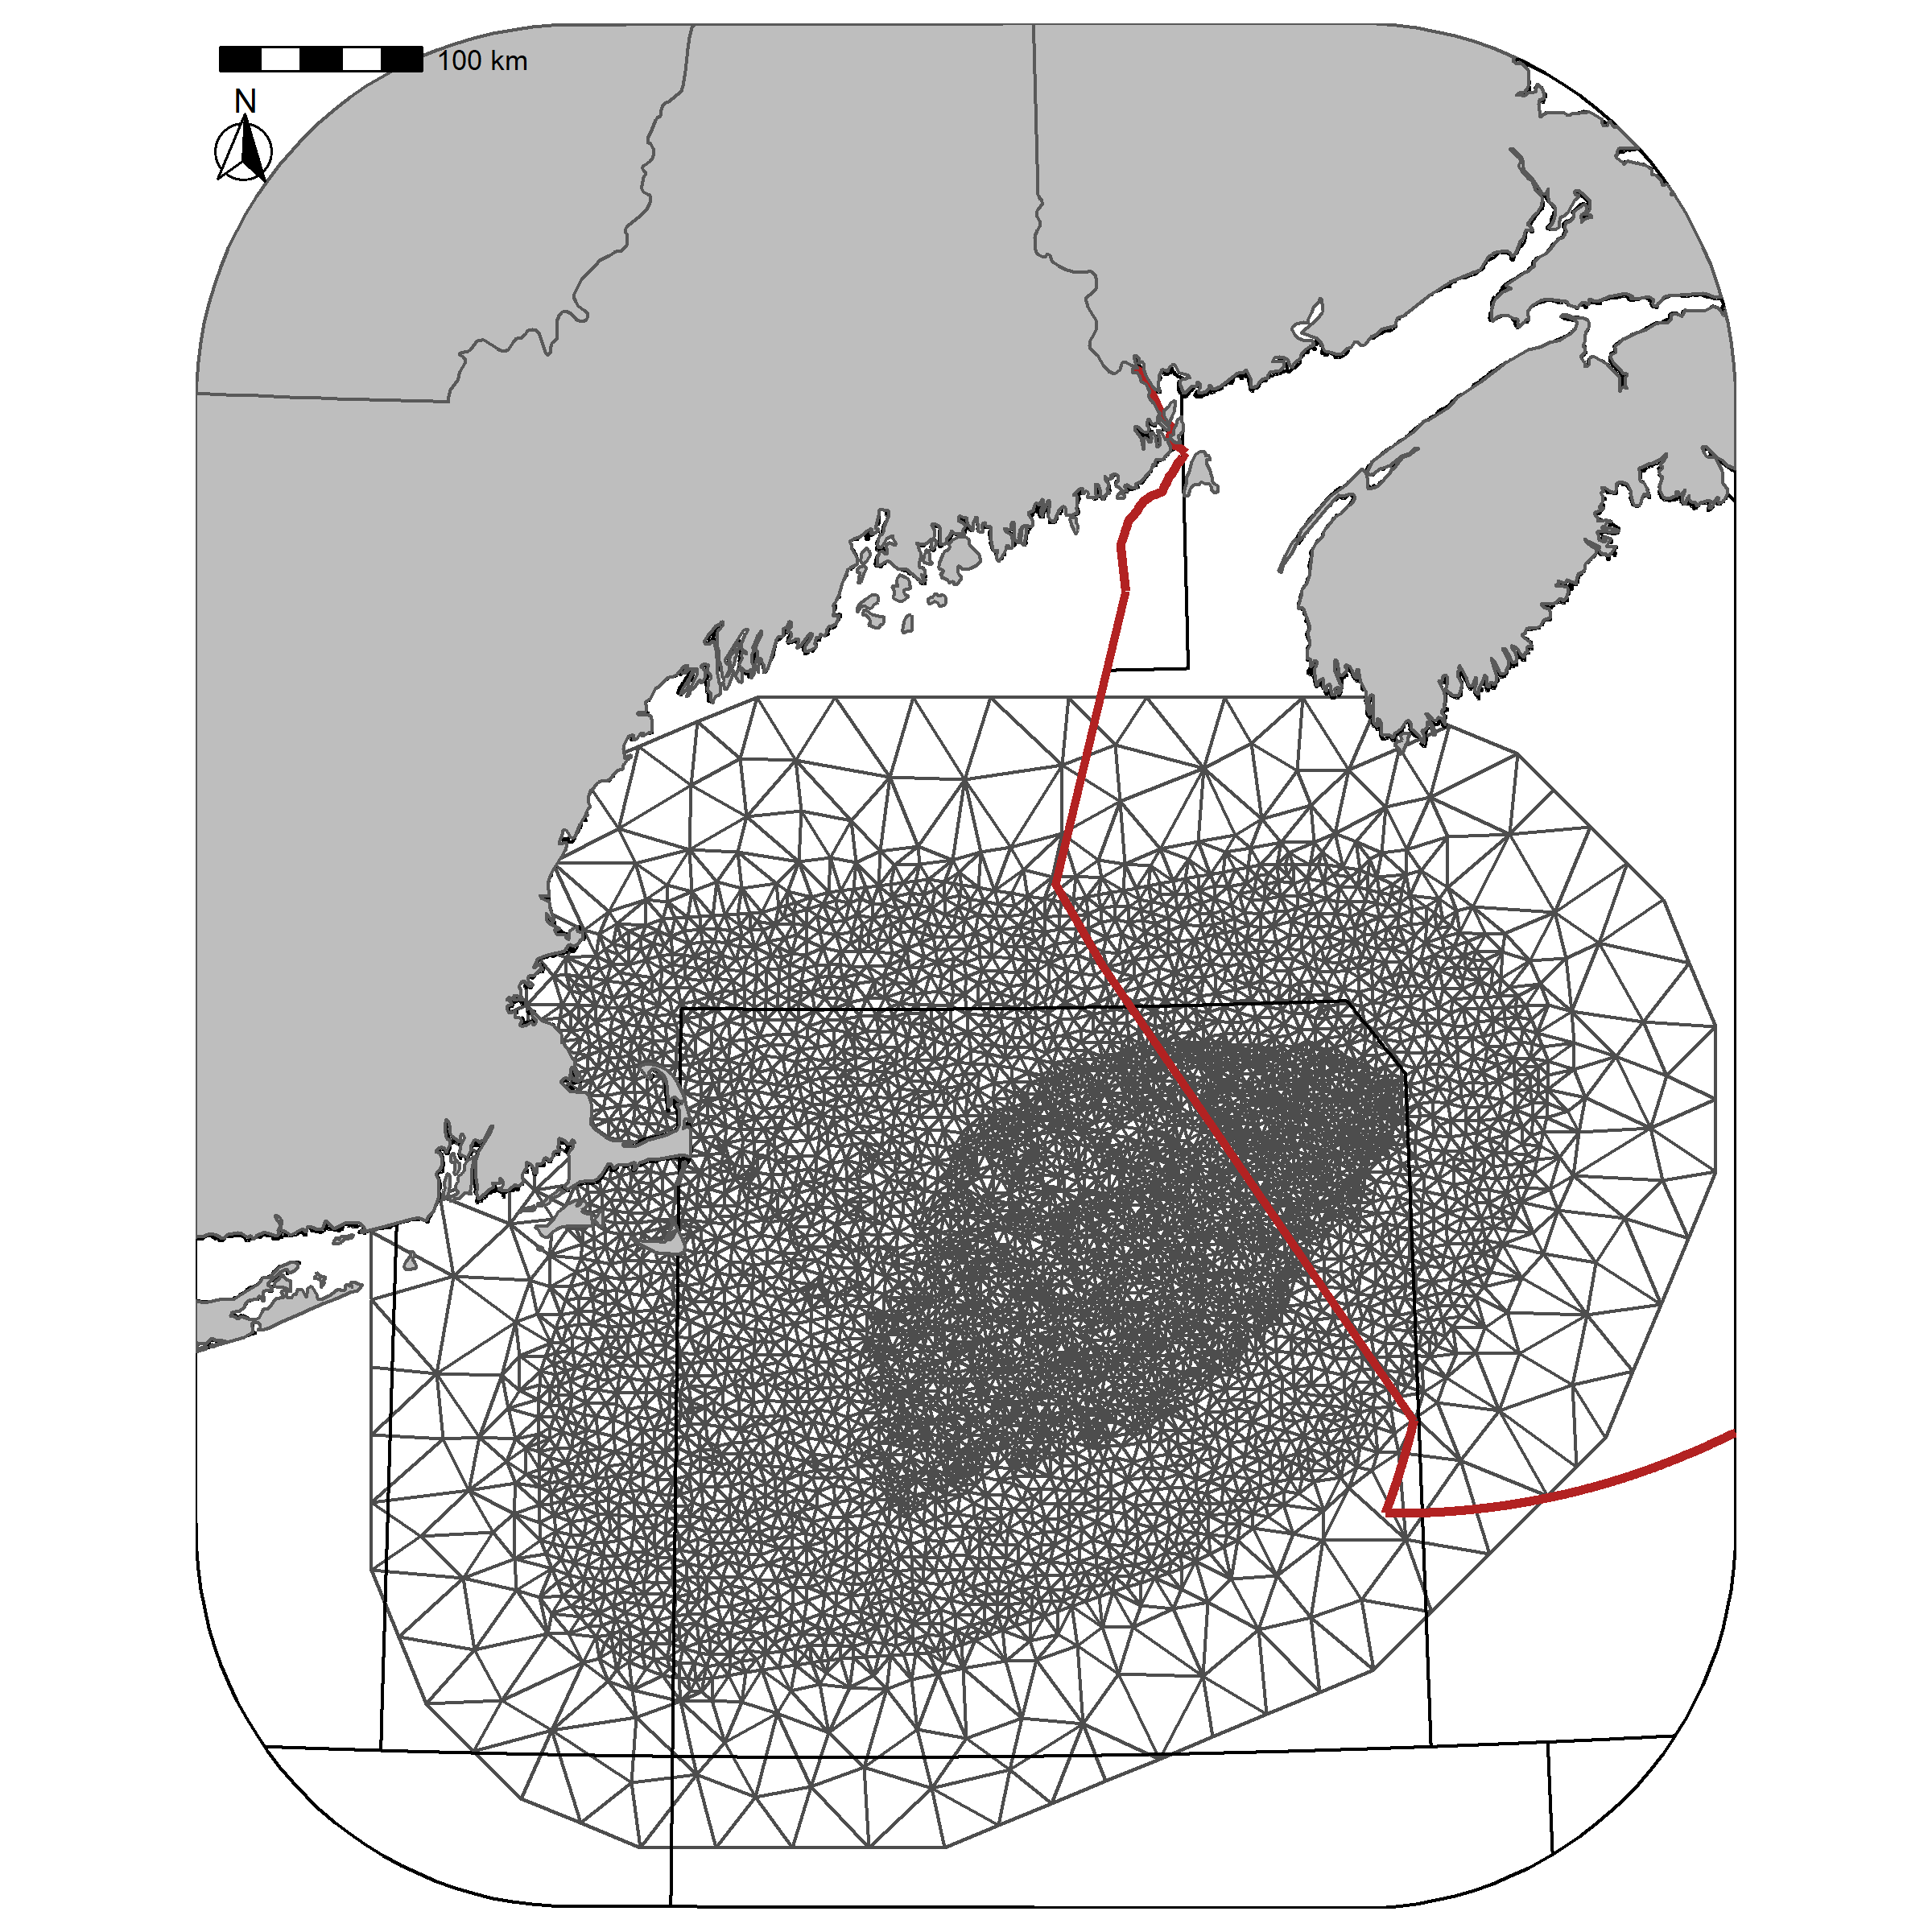
\includegraphics[width=1\linewidth]{D:/Github/Paper_2_SDMs/Results/Figures/mesh.grid} 

}

\caption{Prediction grid used for prediction of occurrence probability (OP).}\label{fig:mesh-grid}
\end{figure}

\clearpage
\begin{figure}[htb]

{\centering 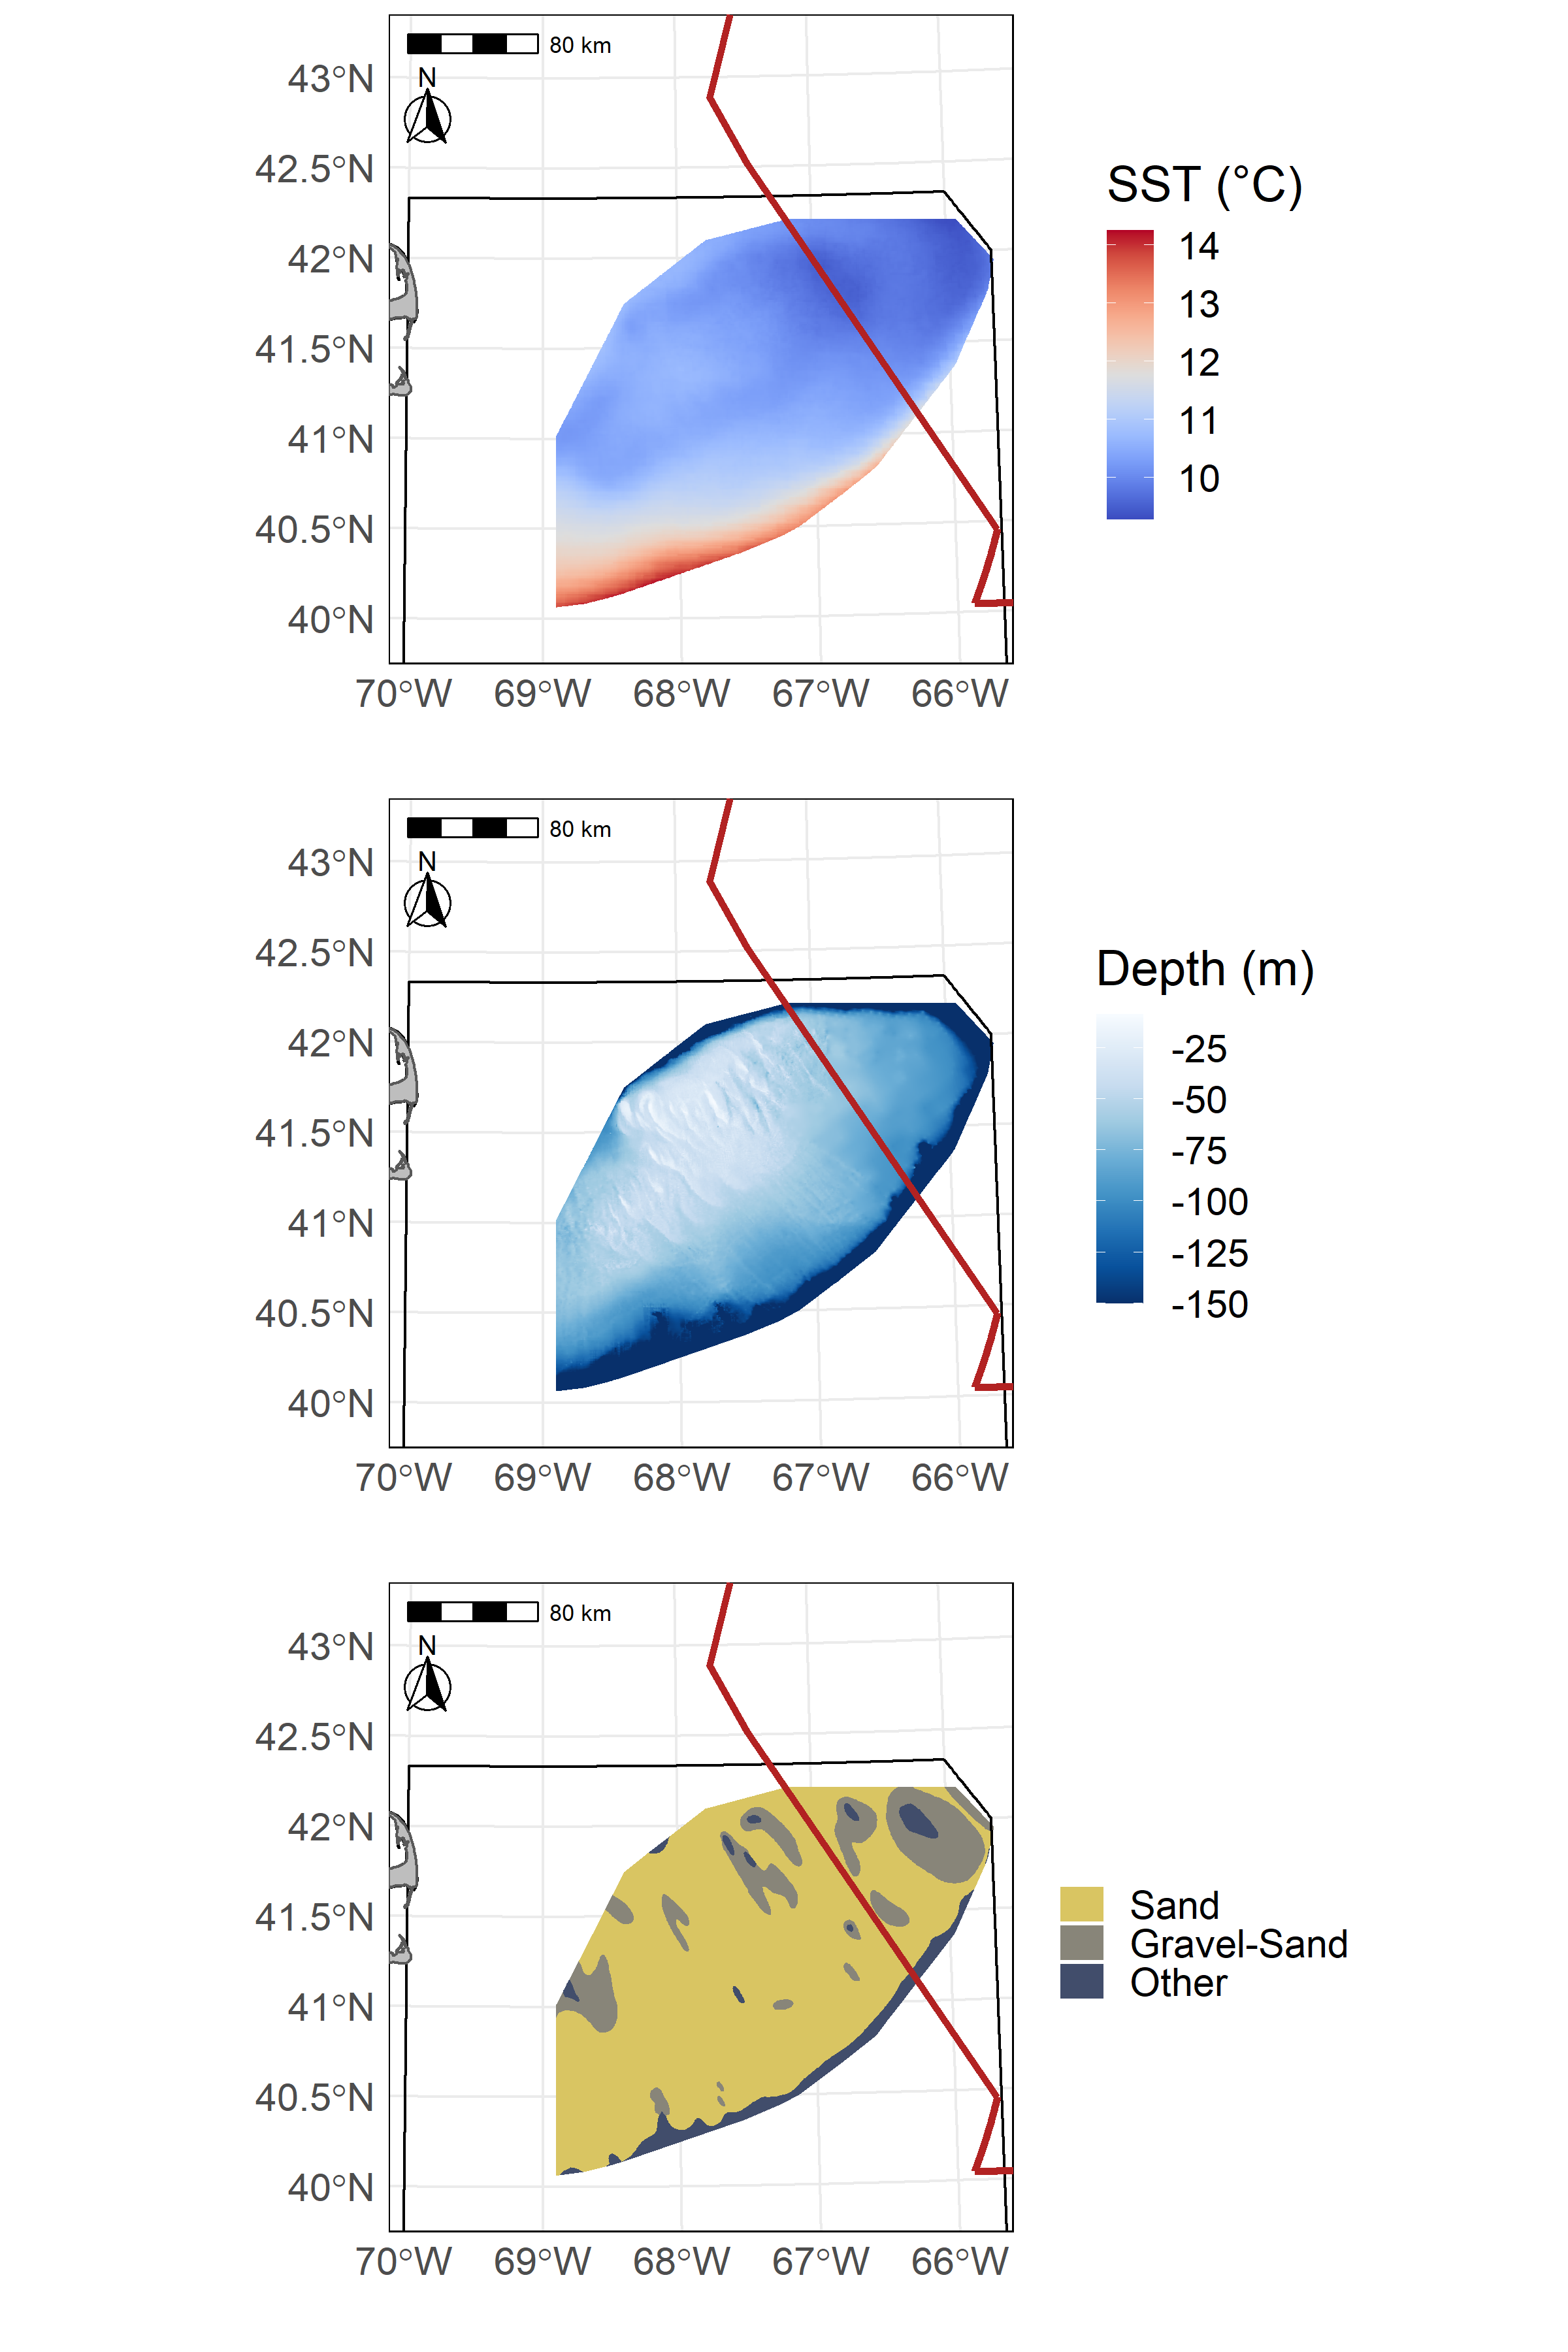
\includegraphics[width=1\linewidth]{D:/Github/Paper_2_SDMs/Results/Figures/depth_sst_sed_fields} 

}

\caption{Average Sea Surface Temperature on Georges Bank (GB) from 1997-2008 (SST in °C) in the top panel, GB bathymetry (depth in meters) in the center panel, and GB sediment type in the bottom panel.}\label{fig:SST-Dep-Sed}
\end{figure}

\begin{landscape}
\begin{figure}[htb]

{\centering 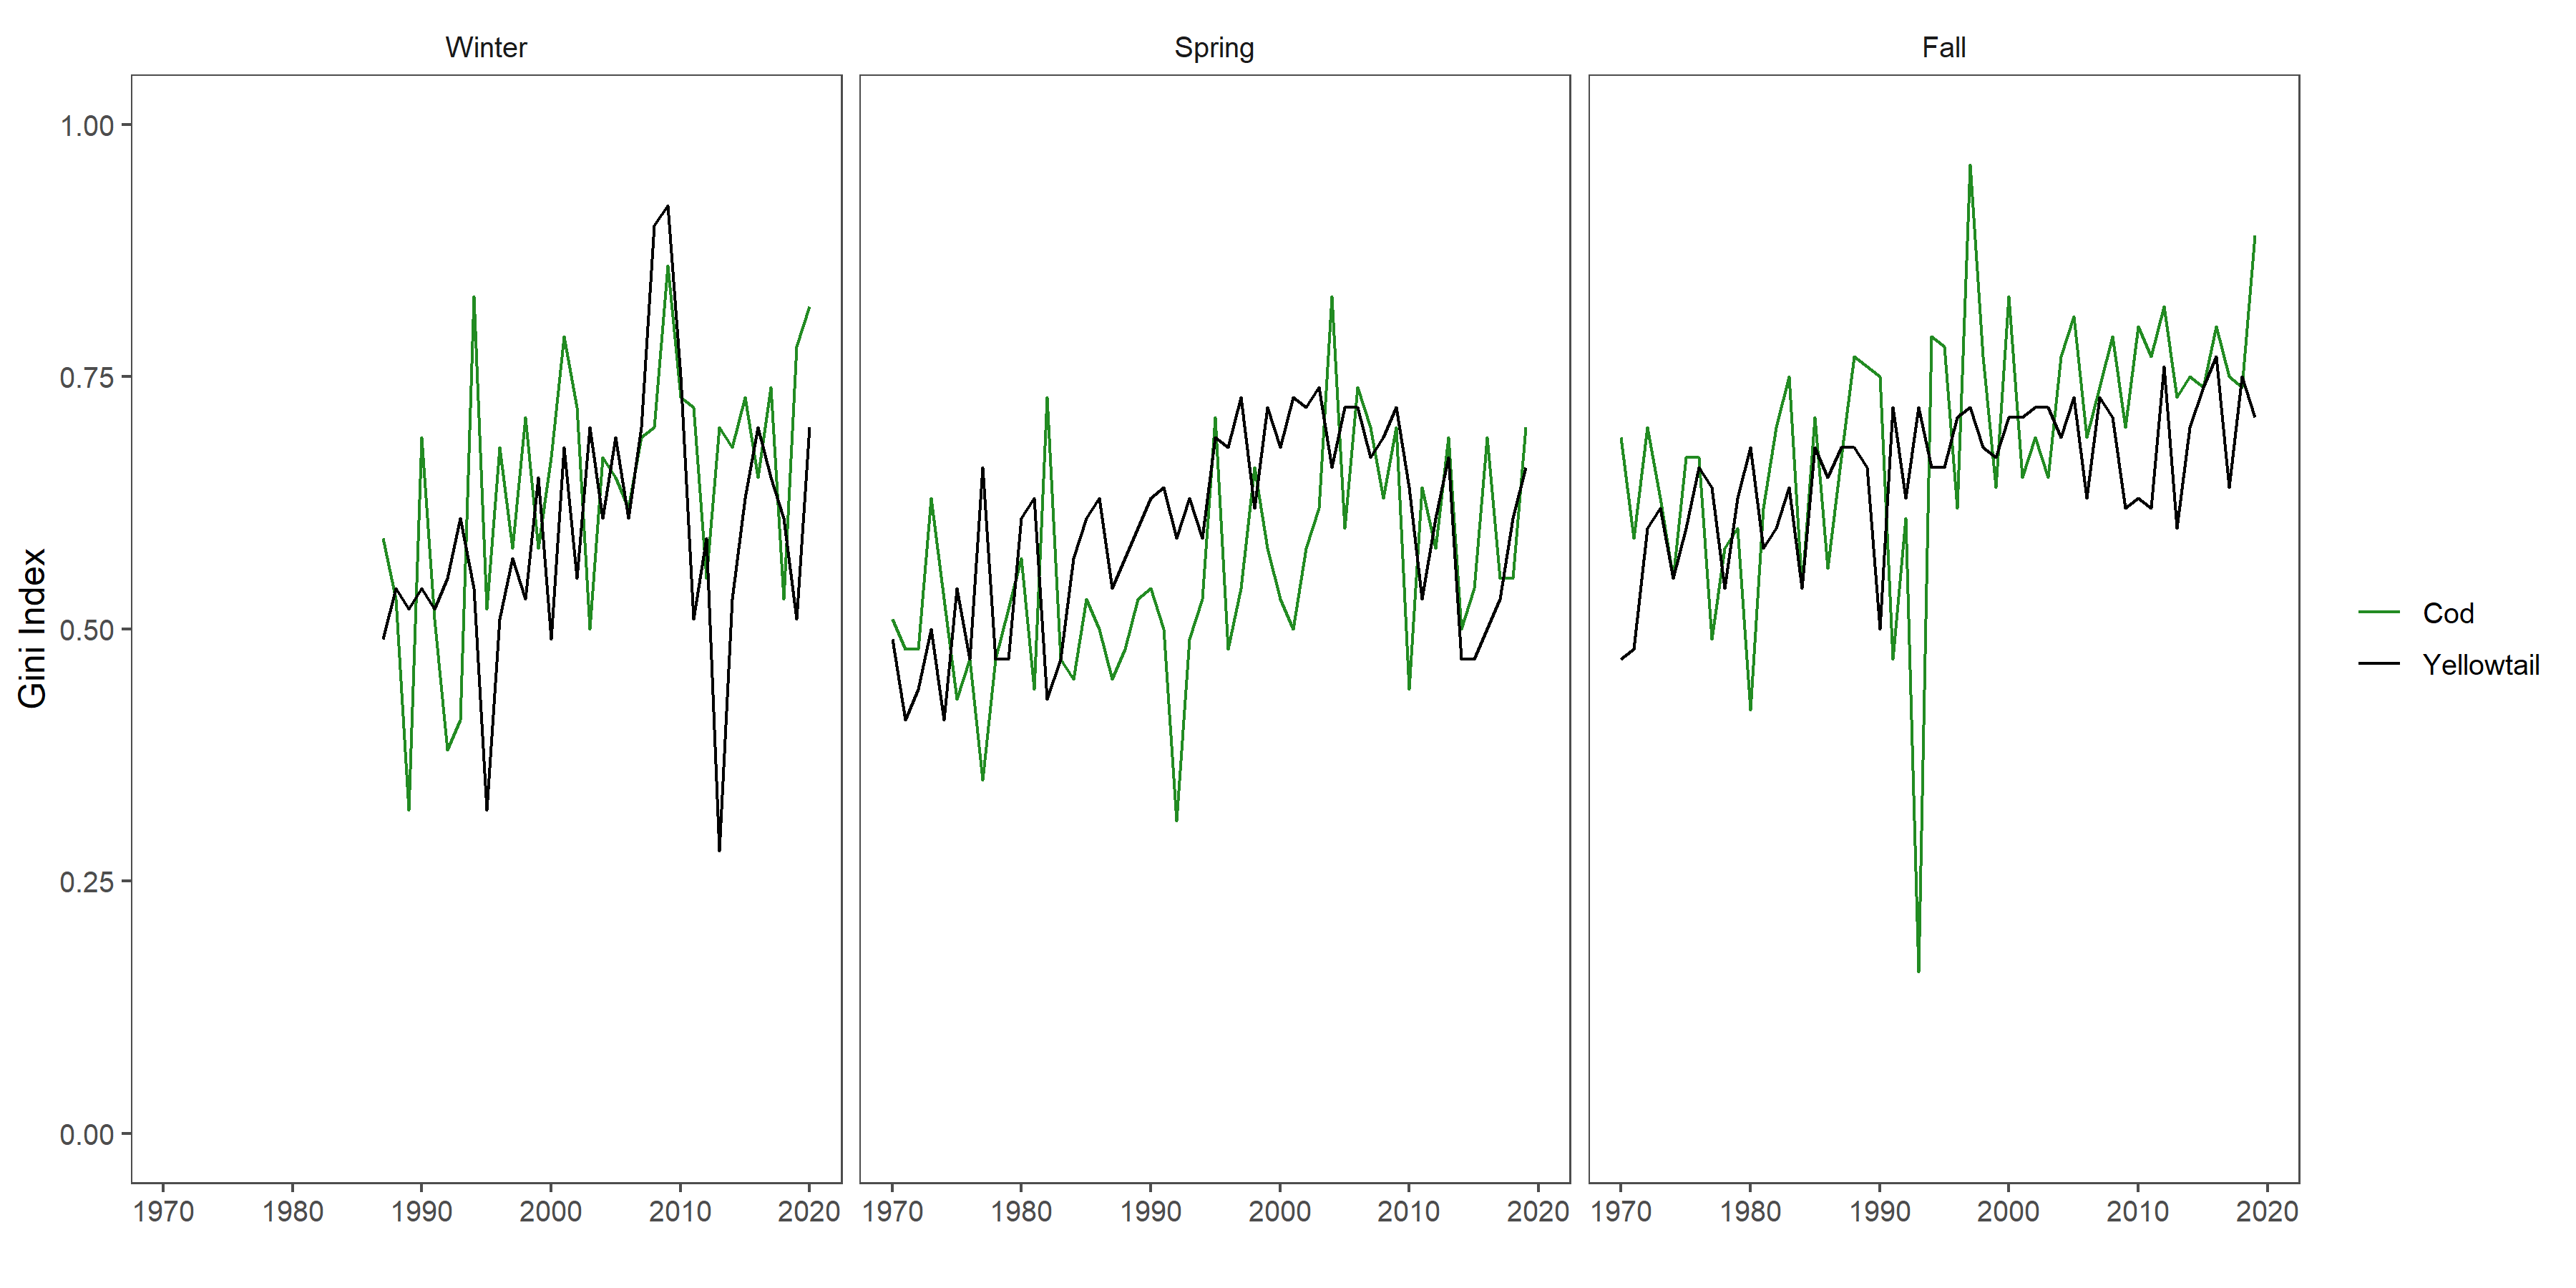
\includegraphics[width=1\linewidth]{D:/Github/Paper_2_SDMs/Results/Figures/Gini_index} 

}

\caption{Gini Index }\label{fig:gini-index}
\end{figure}

\hypertarget{model-selection}{%
\subsection{Model Selection}\label{model-selection}}

Stage 1 of model selection resulted in a significant reduction in the number of covariates. For Atlantic Cod, sea surface temperature (\emph{SST}) was identified as a significant covariate in the Winter and Spring, in addition depth (\emph{Dep}) and stratification were also significant predictors in the Spring. In the Fall no covariates had a WAIC that were a significant improvement from the intercept only model (Figure \ref{fig:diag-1-fe}). Further model selection indicated that an additive \emph{Dep + SST} model was the preferred model in all 3 seasons for Atlantic Cod (Figures \ref{fig:diag-2-fe} and \ref{fig:diag-3-fe}). When exploring the effect of temporal variability on the random fields, the models using the 5-year random field had the lowest WAIC in all seasons (Figure \ref{fig:diag-rf}).

For Yellowtail Flounder, stage 1 of model selection indicated that the inclusion of \emph{Dep} significantly improved the models in all 3 seasons (surveys), while Sediment type (\emph{Sed}) and chlorophyll concentration (\emph{Chl}) in the Fall had a similar impact on the model WAIC as \emph{Dep}. As a result \emph{SST}, \emph{Dep}, \emph{Chl}, and \emph{Sed} were used to explore the development of more complex covariate models. For Yellowtail Flounder the best models in stage 2 of model selection included 2 covariates with a combination of Dep, SST, and Sed (Figure \ref{fig:diag-2-fe}). Further model selection indicated that the preferred model for Yellowtail Flounder in all 3 seasons was an additive model including \emph{Dep}, \emph{SST}, and \emph{Sed} (Figure \ref{fig:diag-3-fe}). When exploring the effect of temporal variability on the random fields, the 3-year field had the lowest WAIC in the Winter and Spring, while the 5-year field had the lowest WAIC in the Fall (Figure \ref{fig:diag-rf}). Additional model selection results are available in the Model Output and Model Diagnostics sections of the interactive dashboard (\url{https://github.com/Dave-Keith/Paper_2_SDMs/tree/master/Dashboard}).

\newpage
\begin{figure}[htb]

{\centering 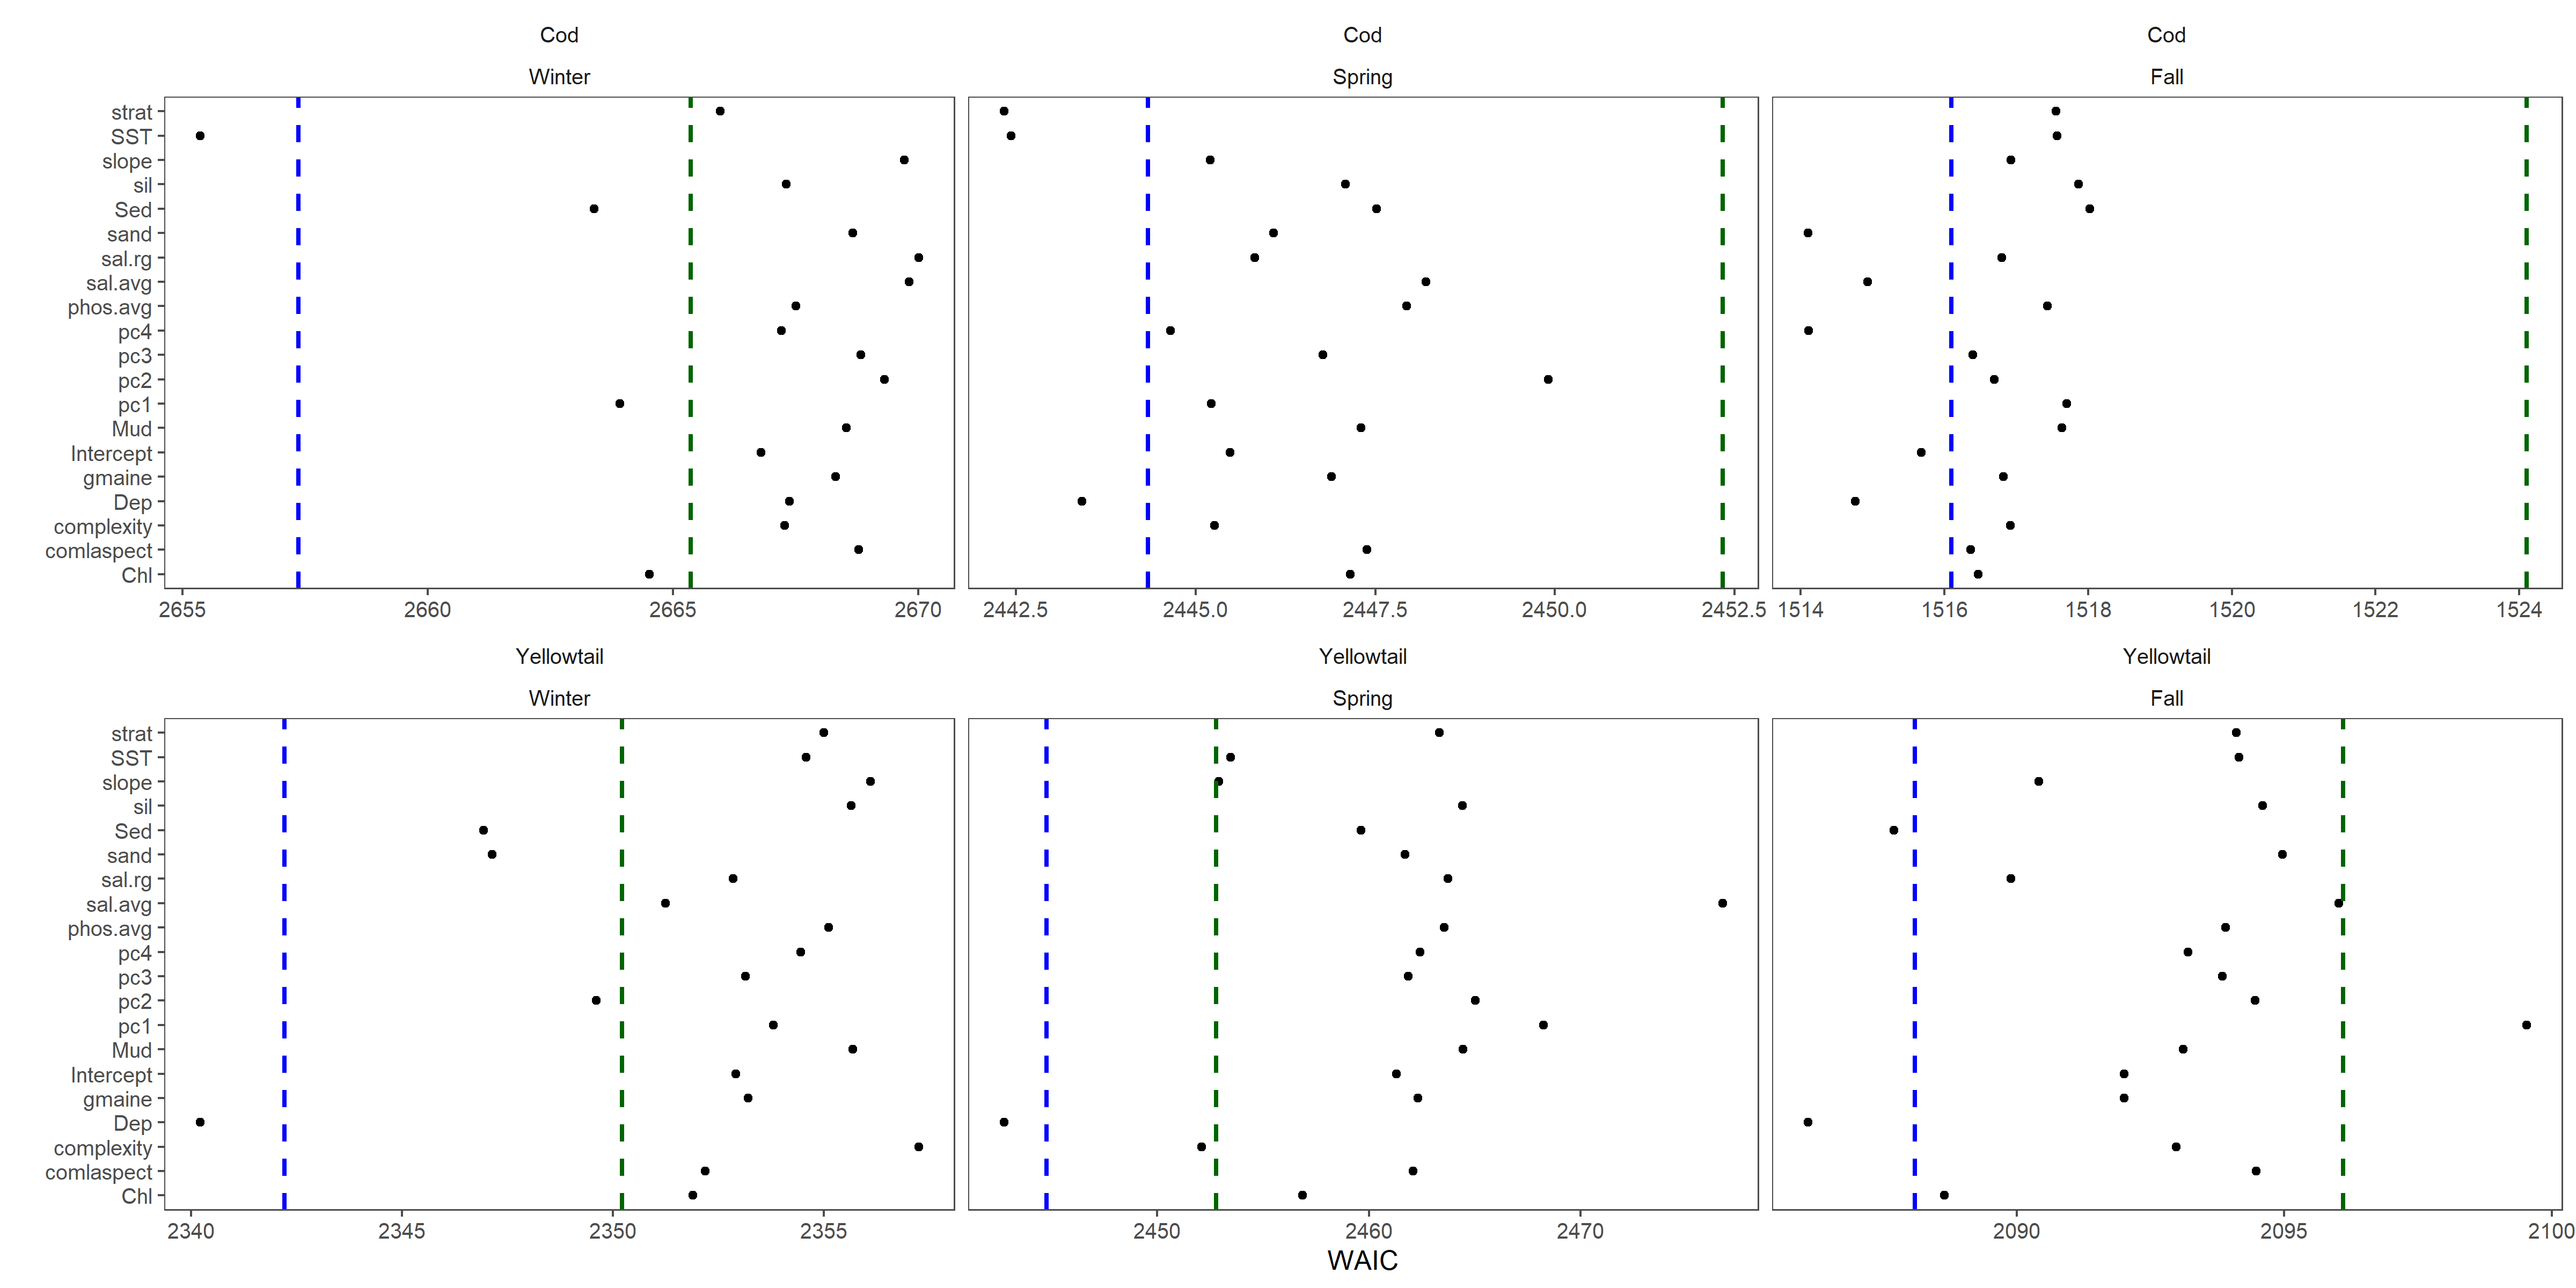
\includegraphics[width=1\linewidth]{D:/Github/Paper_2_SDMs/Results/Figures/Diagnostics_single_fe_waic} 

}

\caption{Initial stage of forward model selection using each of the environmental covariates individually.  This model selection was done using a static random field. Blue dashed line represents 2 WAIC units larger than the preferred model, the red dashed line is 10 WAIC units larger than the preferred model WAIC. }\label{fig:diag-1-fe}
\end{figure}

\newpage
\begin{figure}[htb]

{\centering 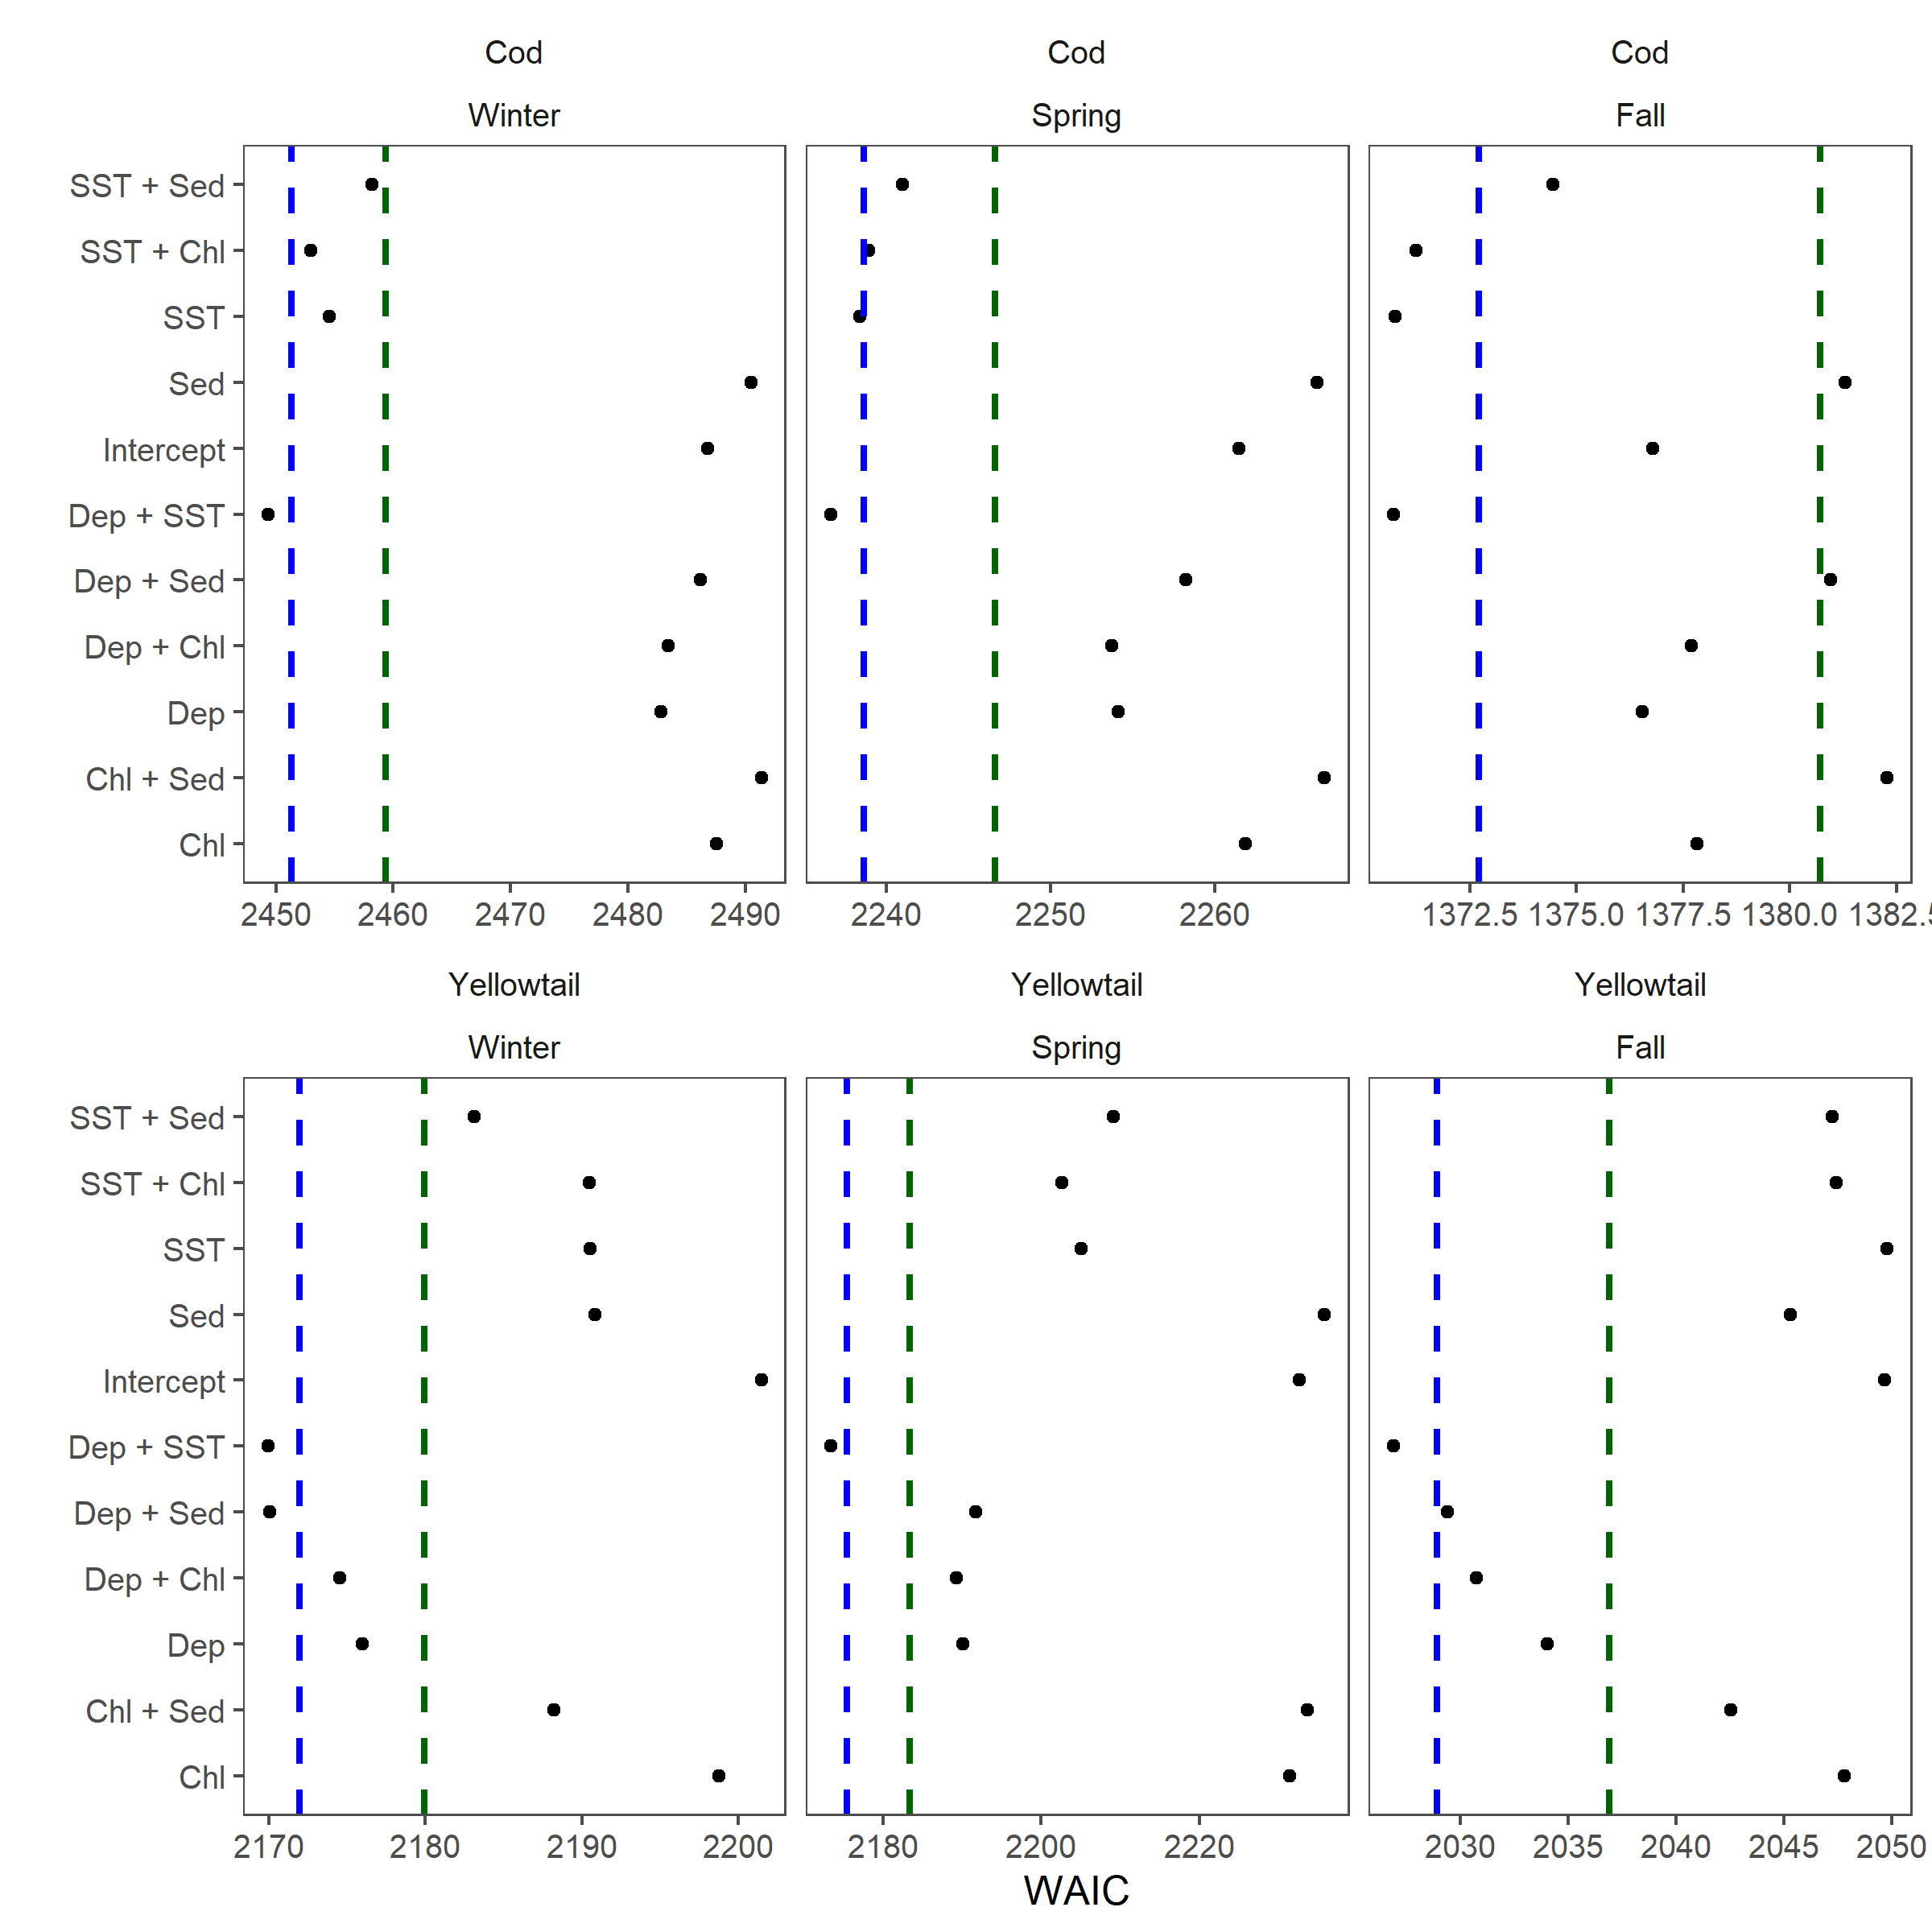
\includegraphics[width=1\linewidth]{D:/Github/Paper_2_SDMs/Results/Figures/Diagnostics_2_covars_fe_waic} 

}

\caption{Stage 2 of model selection including additive models with 2 covariates based on the covariates identified in the initial model selection stage. These models were compared using the 10-year random field models. Blue dashed line represents 2 WAIC units larger than the preferred model, the red dashed line is 10 WAIC units larger than the preferred model WAIC.}\label{fig:diag-2-fe}
\end{figure}

\newpage
\begin{figure}[htb]

{\centering 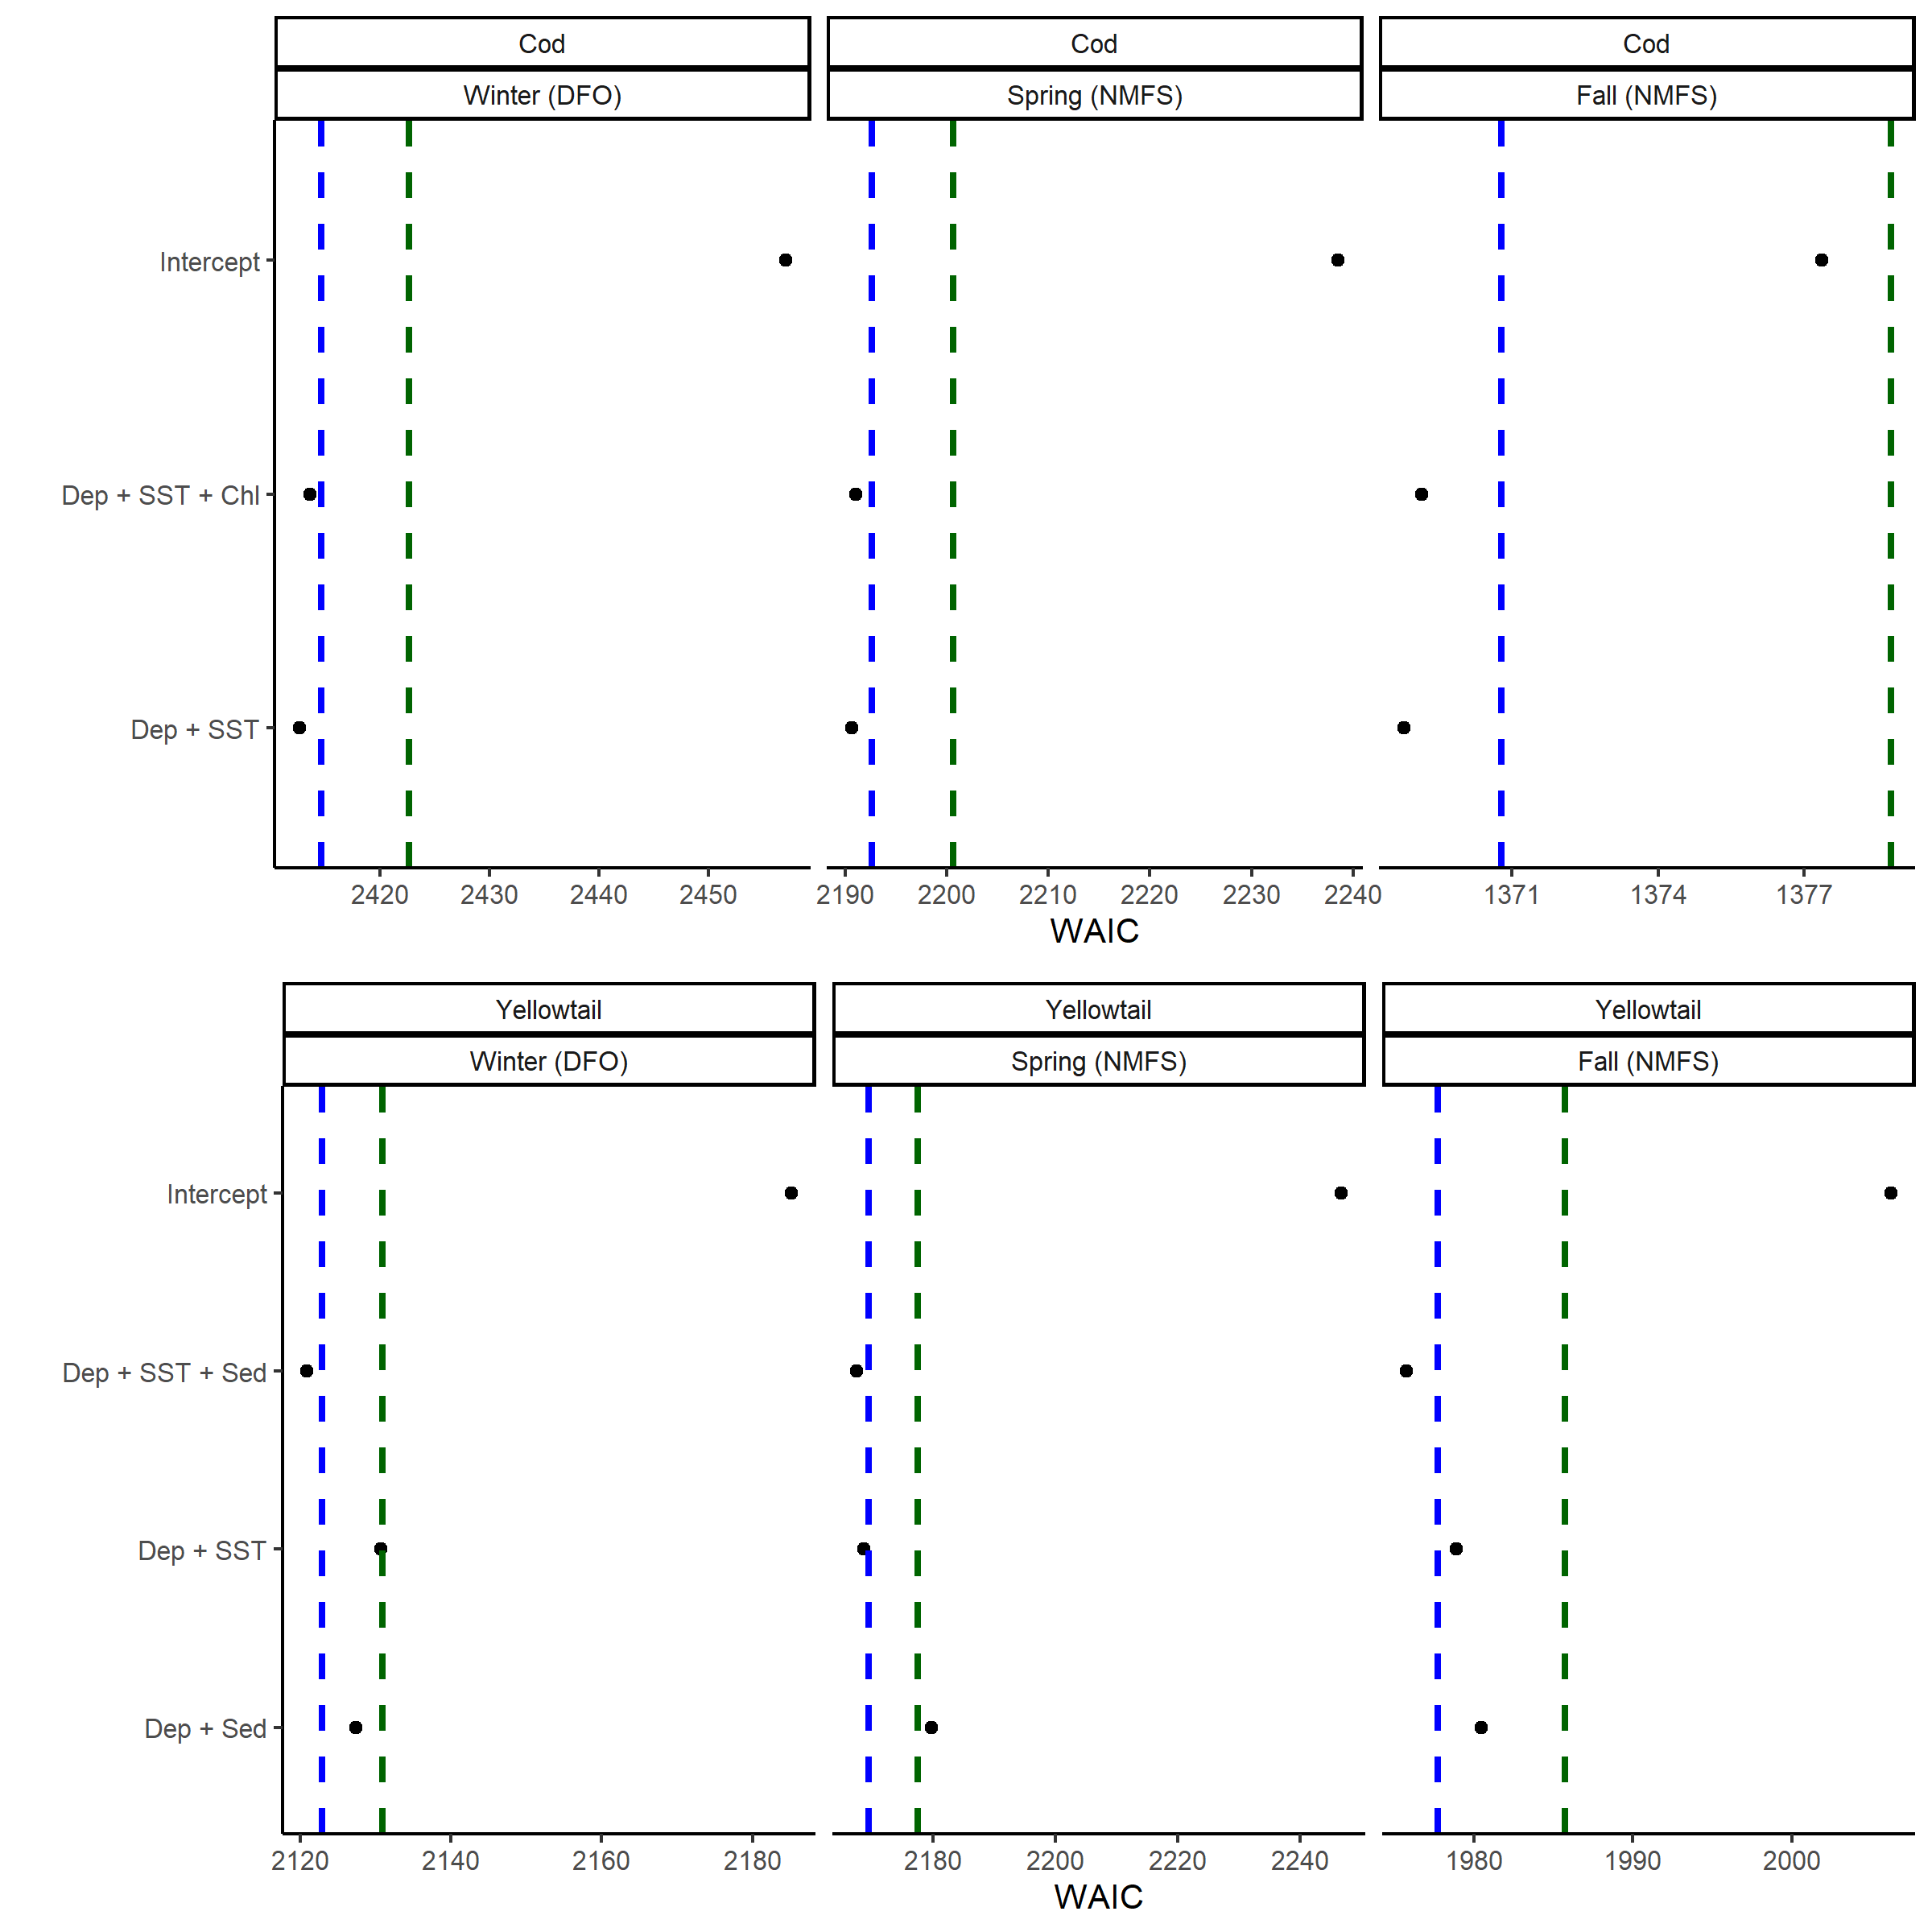
\includegraphics[width=1\linewidth]{D:/Github/Paper_2_SDMs/Results/Figures/Diagnostics_3_covars_fe_waic} 

}

\caption{Final stage of covariate model selection which includes model with up to 3 covariate terms based on models selected at stage 2. Blue dashed line represents 2 WAIC units larger than the preferred model, the red dashed line is 10 WAIC units larger than the preferred model WAIC.}\label{fig:diag-3-fe}
\end{figure}

\newpage
\begin{figure}[htb]

{\centering 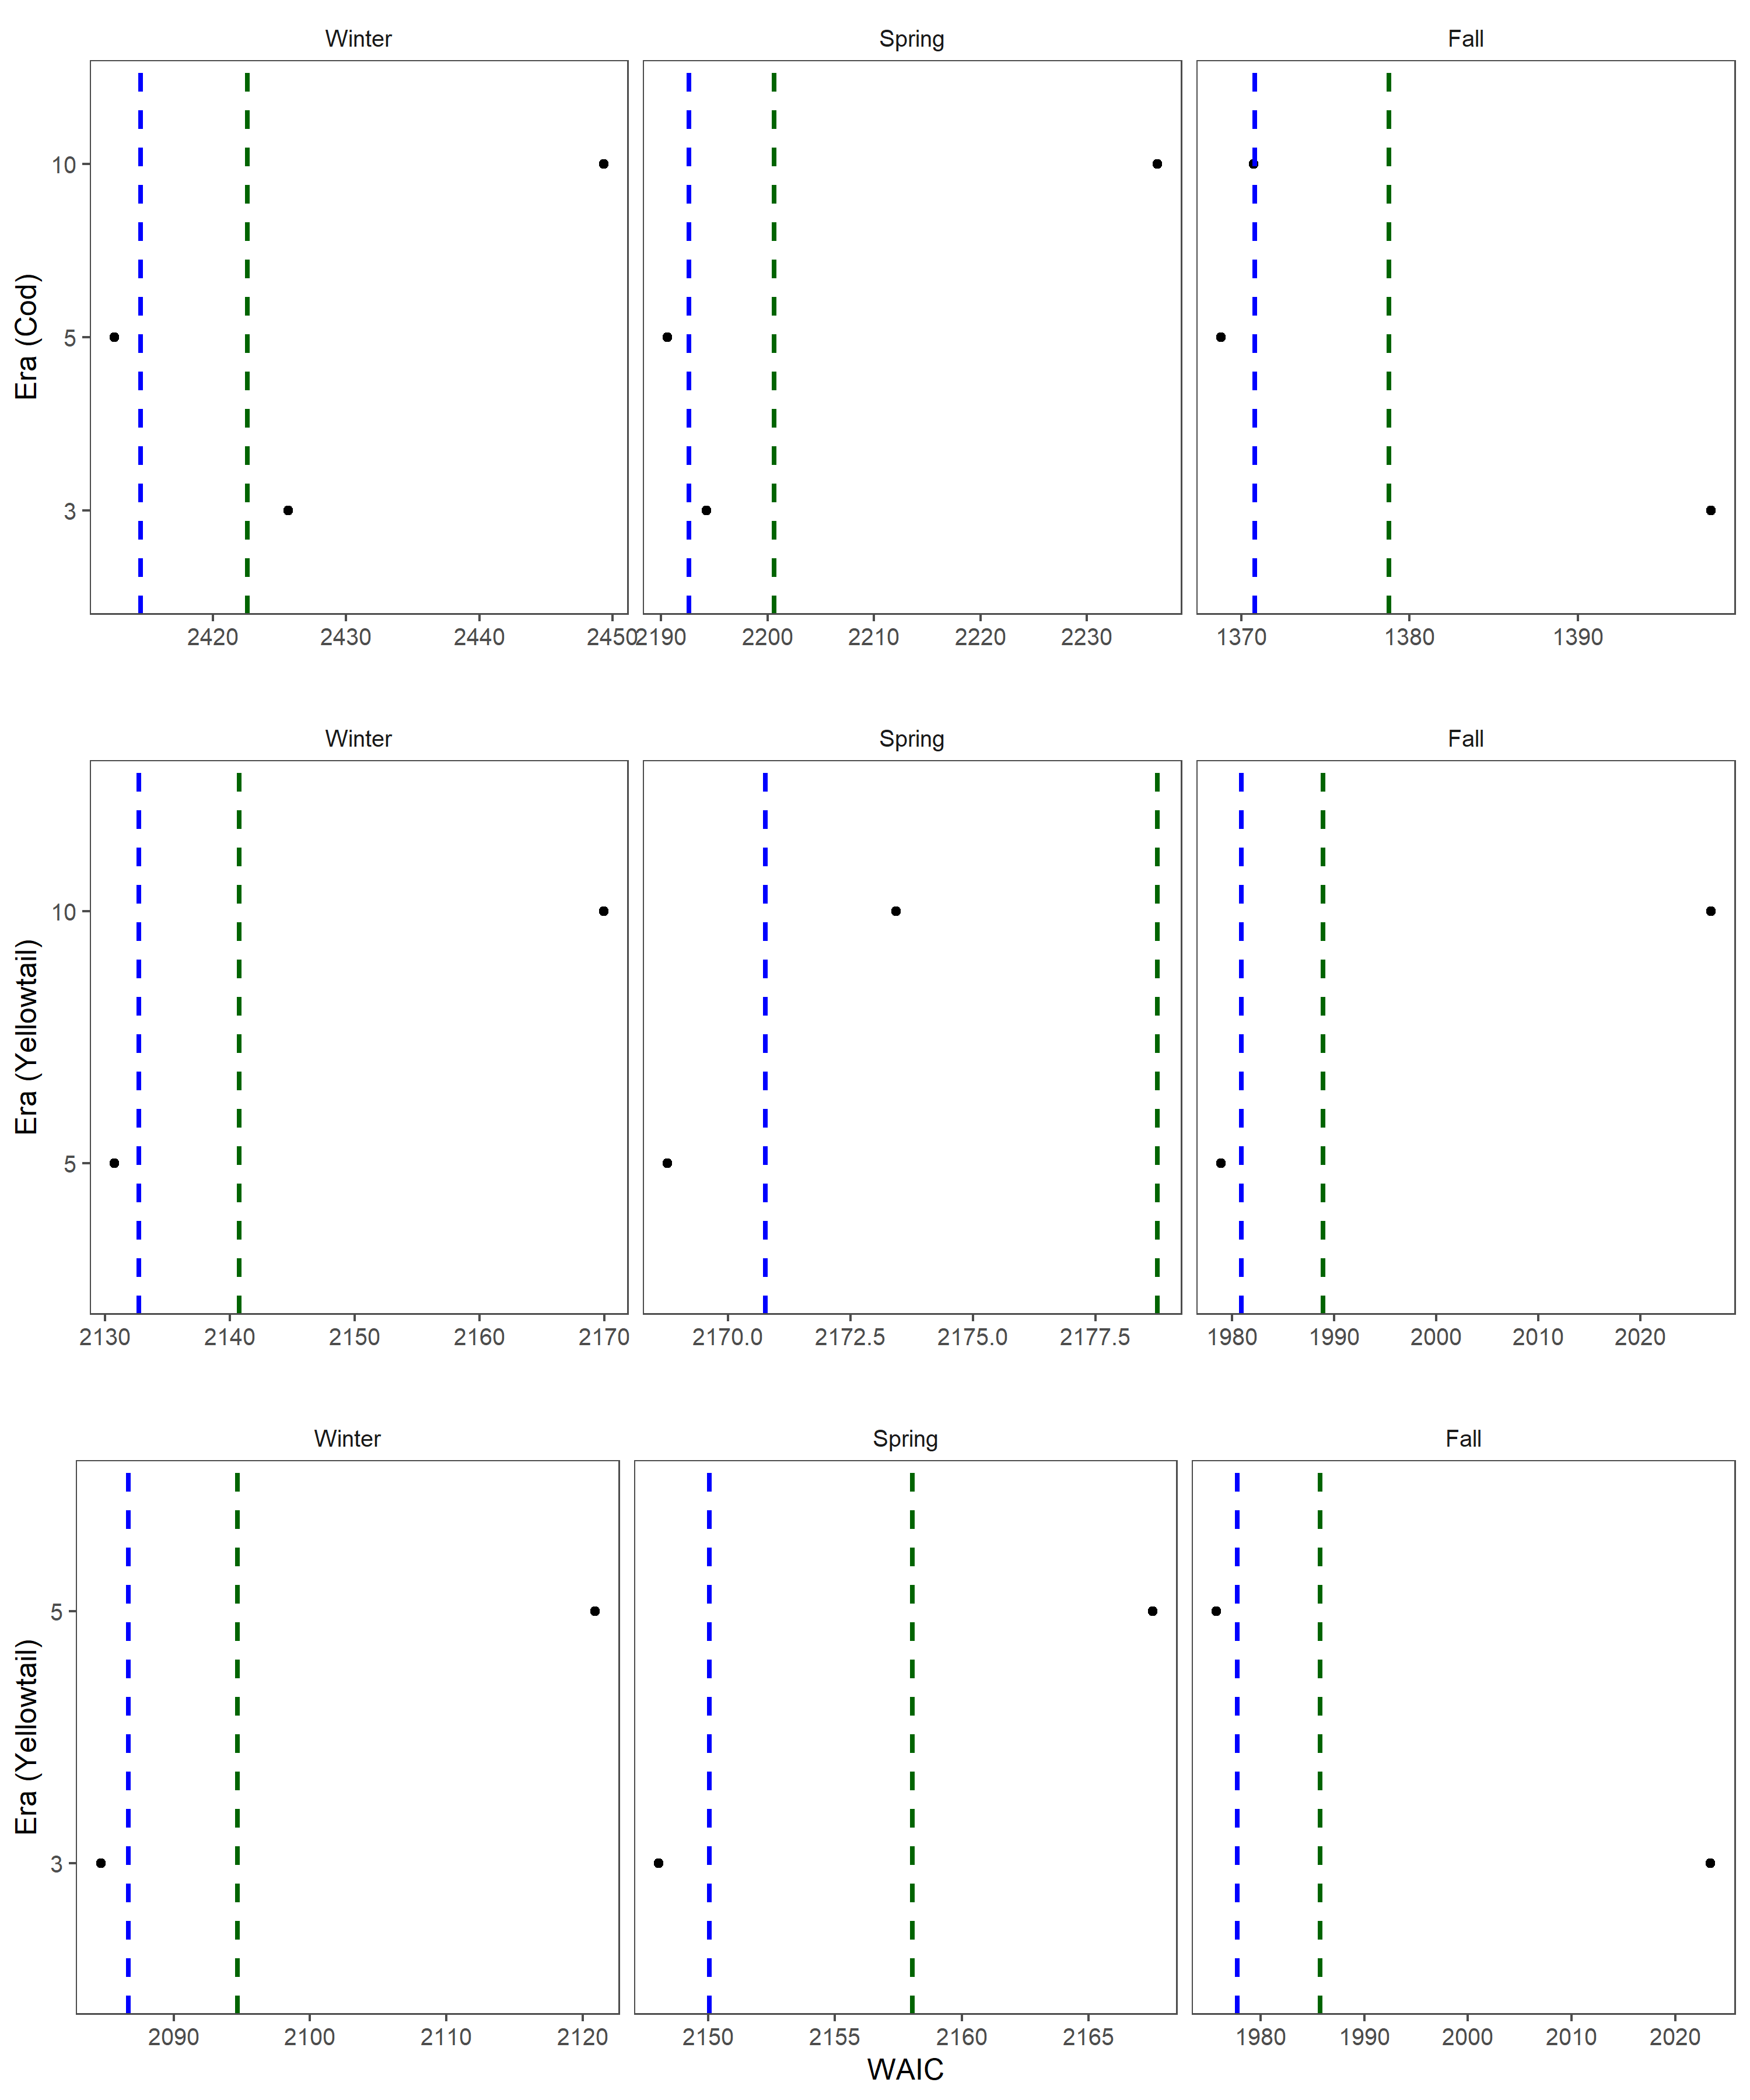
\includegraphics[width=1\linewidth]{D:/Github/Paper_2_SDMs/Results/Figures/Diagnostics_rf_waic} 

}

\caption{Model selection comparing the random fields models.  For cod the model used is Dep + SST for all of the random fields.  For Yellowtail the 5 and 10 year random fields were compared using the Dep + SST model, while the 5 and 3 fields were compared using the slightly preferred Dep + SST + Sed model. Blue dashed line represents 2 WAIC units larger than the preferred model, the red dashed line is 10 WAIC units larger than the preferred model WAIC.}\label{fig:diag-rf}
\end{figure}
\end{landscape}

\clearpage

\hypertarget{predicted-occurance-probability}{%
\section{Predicted Occurance Probability}\label{predicted-occurance-probability}}

The modelled OP for Atlantic Cod in the Winter and Spring was elevated on all but the most southern portion of GB in the 1970s and 1980s, in the early 1990s there was an abrupt decline in the OP throughout much of the U.S. portion of GB, while OP remained elevated in Canadian waters and in the area straddling the ICJ line (Figures \ref{fig:pf-winter-cod} - \ref{fig:pf-spring-cod}). In the Fall the core areas were isolated to the north of GB. An area on the northwest of GB had some core area until the early 1980s but the OP in this area declined steadily after this time and has had a low OP in the Fall for over 20 years, the highest OP areas remaining during the Fall are along the northern edge of the bank and mostly in Canadian waters (Figure \ref{fig:pf-fall-cod}).

The modelled OP patterns for Yellowtail Flounder on GB are similar in Winter, Spring, and Fall with core area consistently observed in the region straddling the ICJ line in each season and throughout the study period (Figures \ref{fig:pf-winter-yt} - \ref{fig:pf-fall-yt}). A second region along the western border of the bank also has an elevated OP and appears to be connected via a narrow band of varying width to the core area straddling the ICJ line. The core area of Yellowtail Flounder declined in the late 1980s and early 1990s and was relatively stable until 2016 (Figure \ref{fig:pf-fall-yt}).

The SD of the Atlantic Cod prediction field in the Winter and Spring tended to be elevated in the central portion of the bank, and lowest in the south and along the edges of the prediction domain. In the Fall the Atlantic Cod prediction field SD was lowest in the south, with the low SD area expanding to central regions later in the study period (Figures \ref{fig:pf-winter-cod-sd} - \ref{fig:pf-fall-cod-sd}). For Yellowtail Flounder, the SD was consistently low in the part of the region with a core area that straddled the ICJ line in the Winter, Spring and Fall (Figures \ref{fig:pf-winter-yt-sd} - \ref{fig:pf-fall-yt-sd}). Areas surrounding this region displayed an increase in the SD, while a region in the north and along the southern flank of GB had relatively low SDs; these regions also had relatively low OPs (Figures \ref{fig:pf-winter-yt} - \ref{fig:pf-fall-yt} and \ref{fig:pf-winter-yt-sd} - \ref{fig:pf-fall-yt-sd}).

\newpage
\begin{figure}[htb]

{\centering 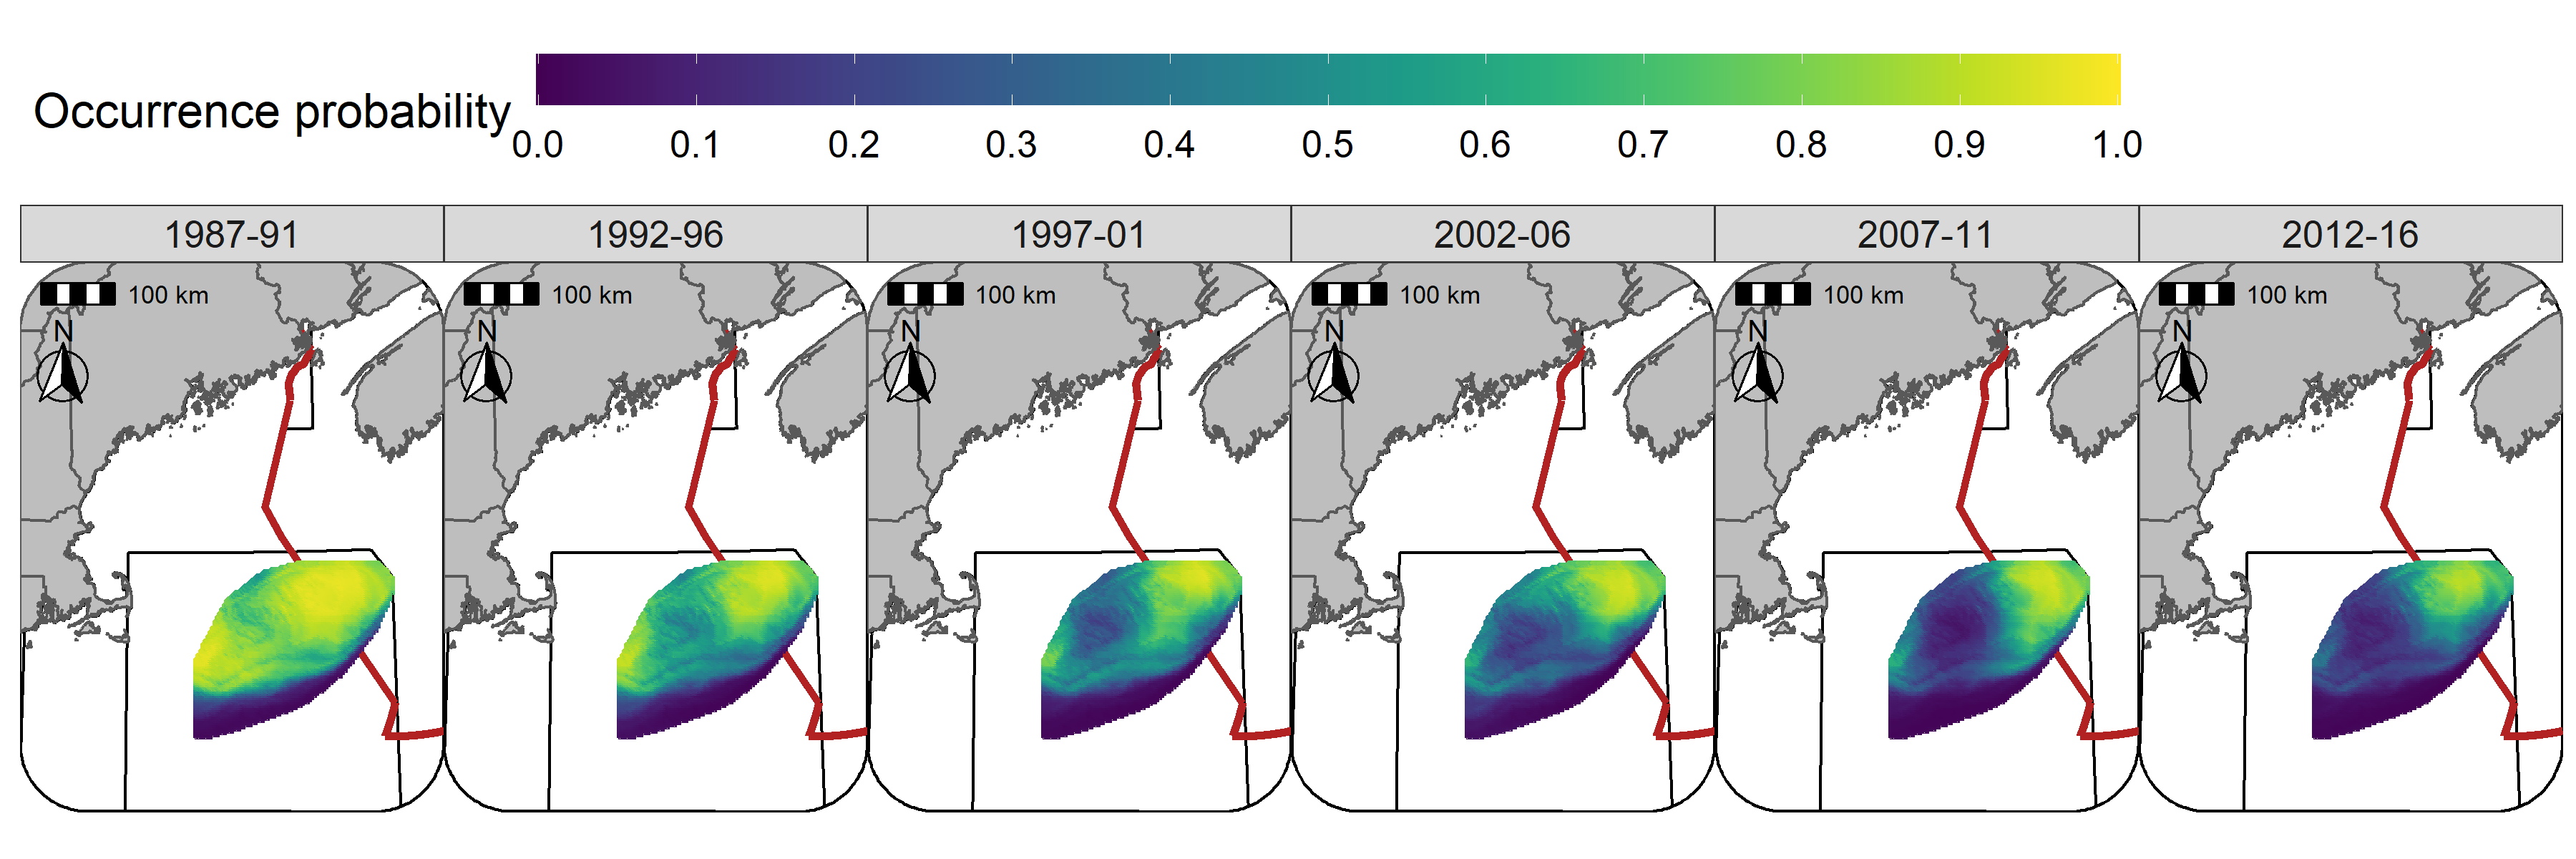
\includegraphics[width=1\linewidth]{D:/Github/Paper_2_SDMs/Results/Figures/pf_winter_cod} 

}

\caption{Predicted occurrence probability for Atlantic Cod  in each era during the Winter (RV survey) using the SST + Depth model and 5 year random field.}\label{fig:pf-winter-cod}
\end{figure}

\newpage
\begin{figure}[htb]

{\centering 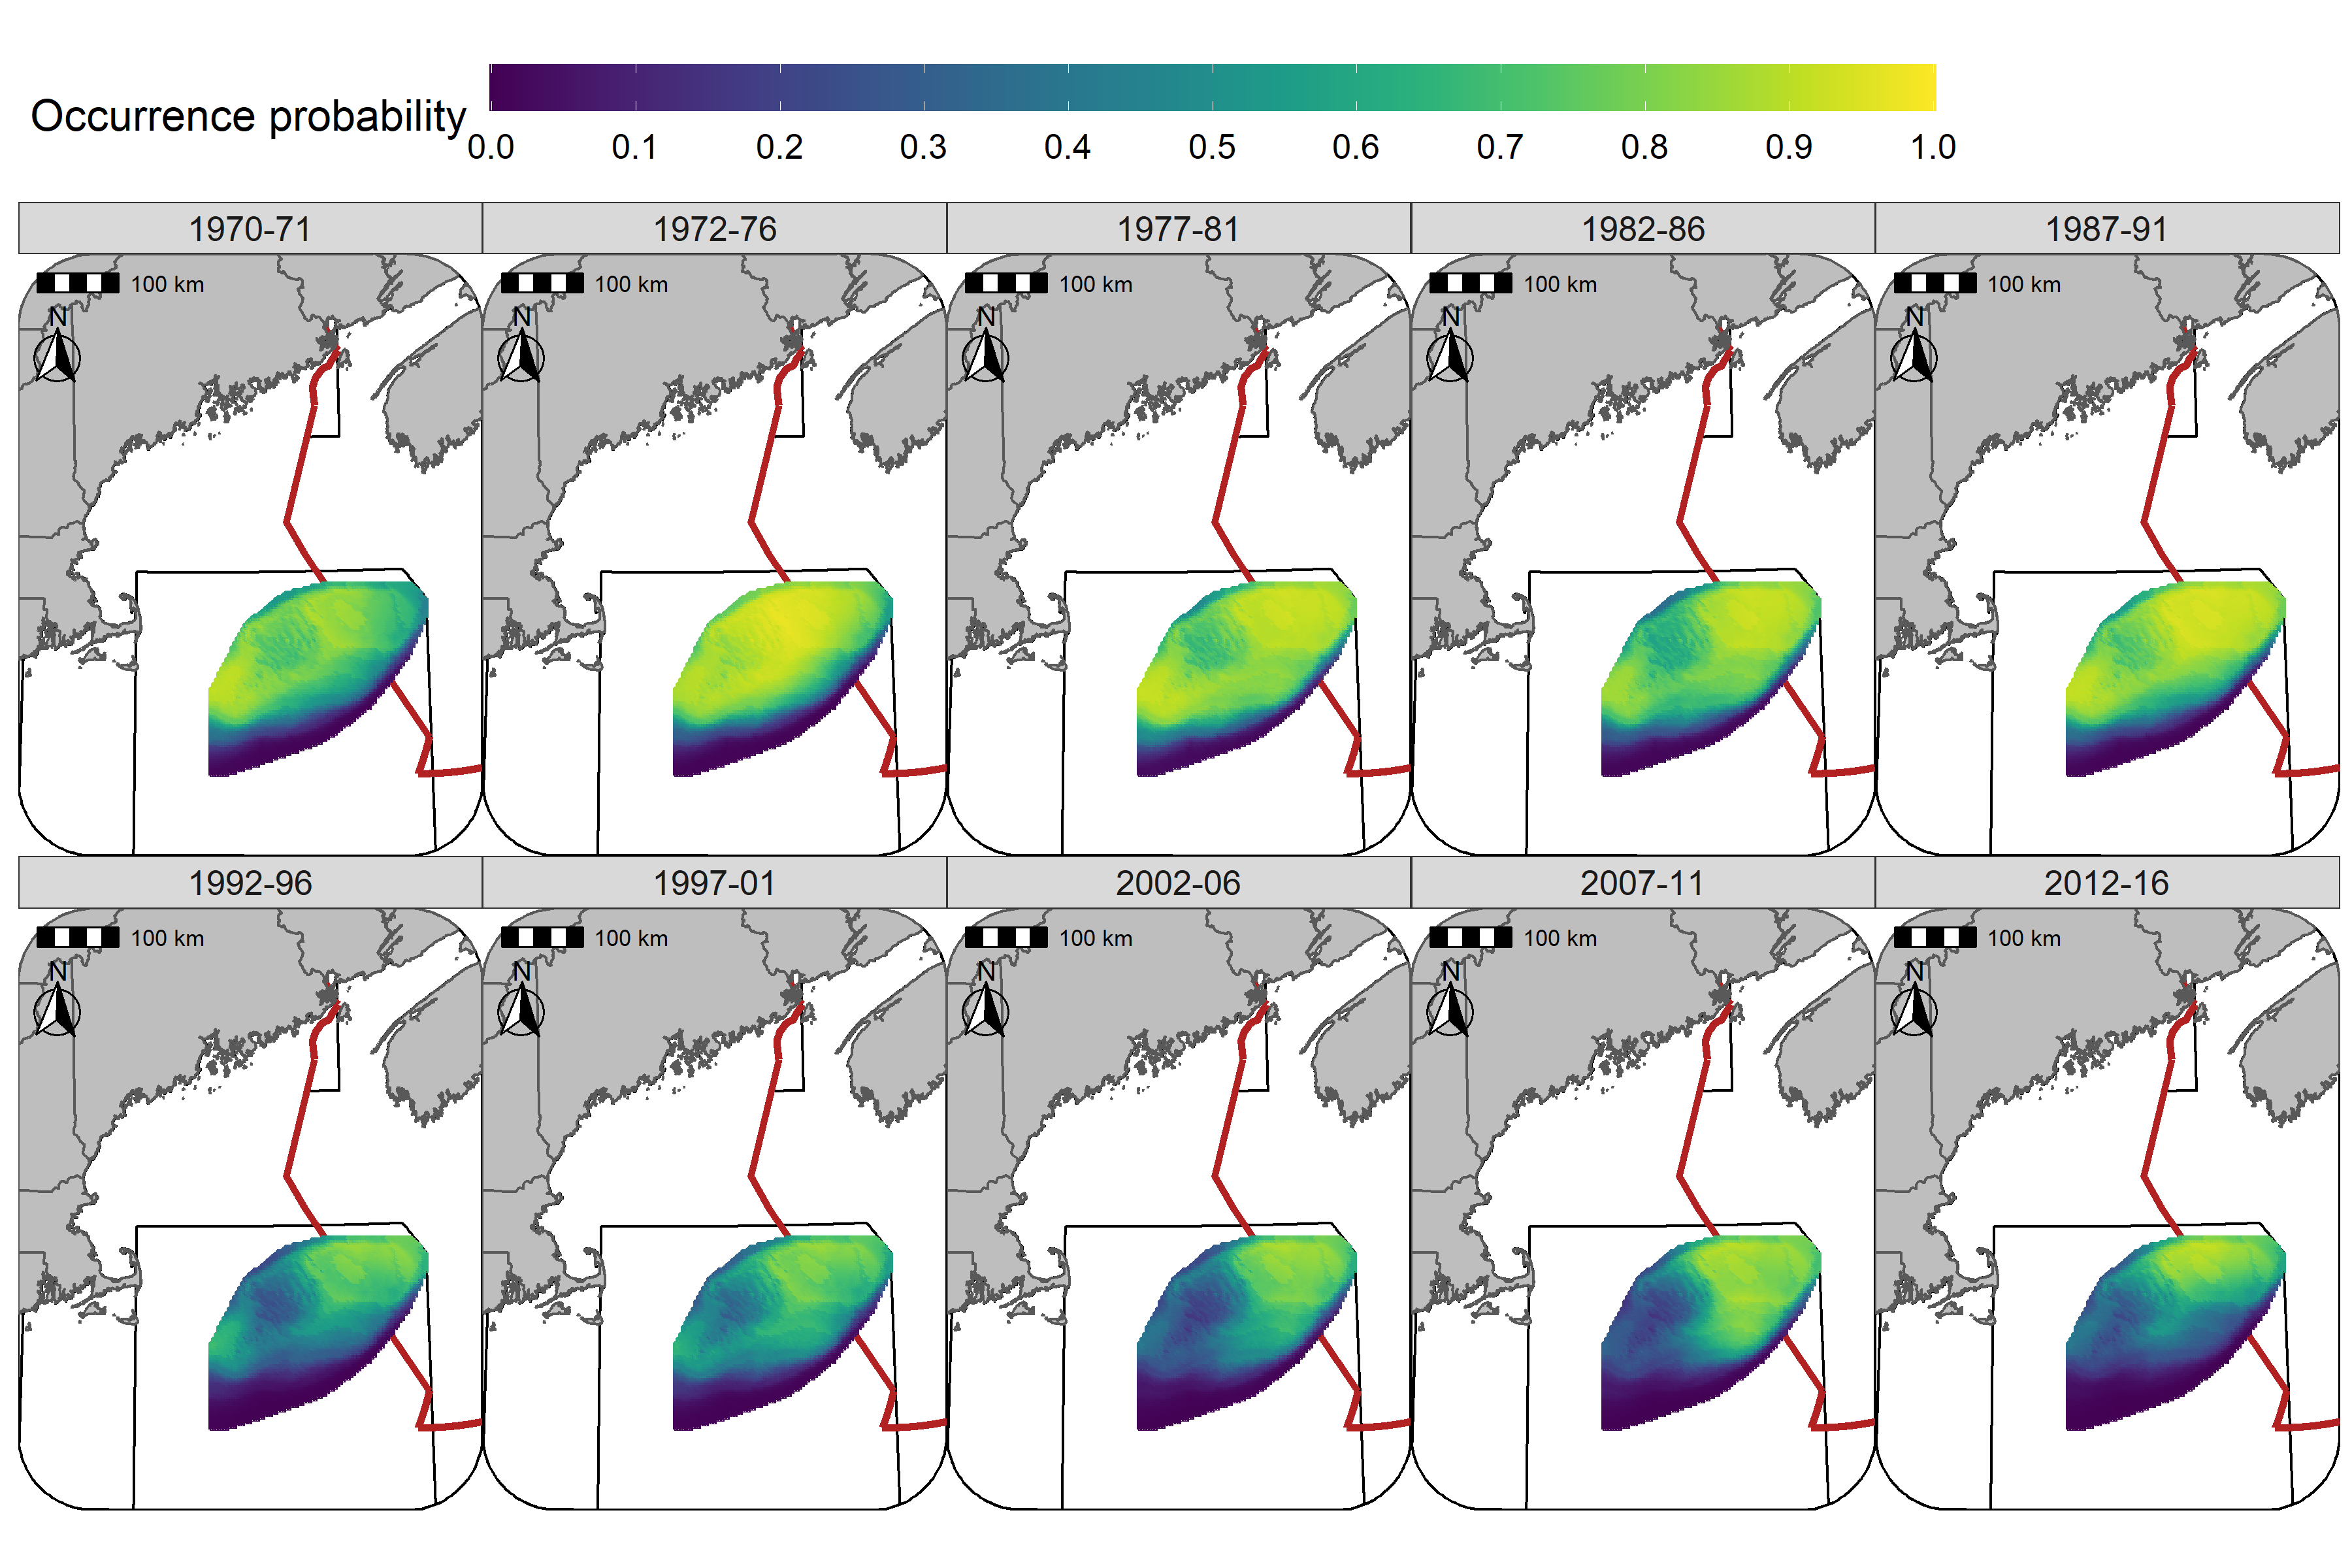
\includegraphics[width=1\linewidth]{D:/Github/Paper_2_SDMs/Results/Figures/pf_spring_cod} 

}

\caption{Predicted occurrence probability for Atlantic Cod  in each era during the Spring (NMFS-spring survey) using the SST + Depth model and 5 year random field.}\label{fig:pf-spring-cod}
\end{figure}

\newpage
\begin{figure}[htb]

{\centering 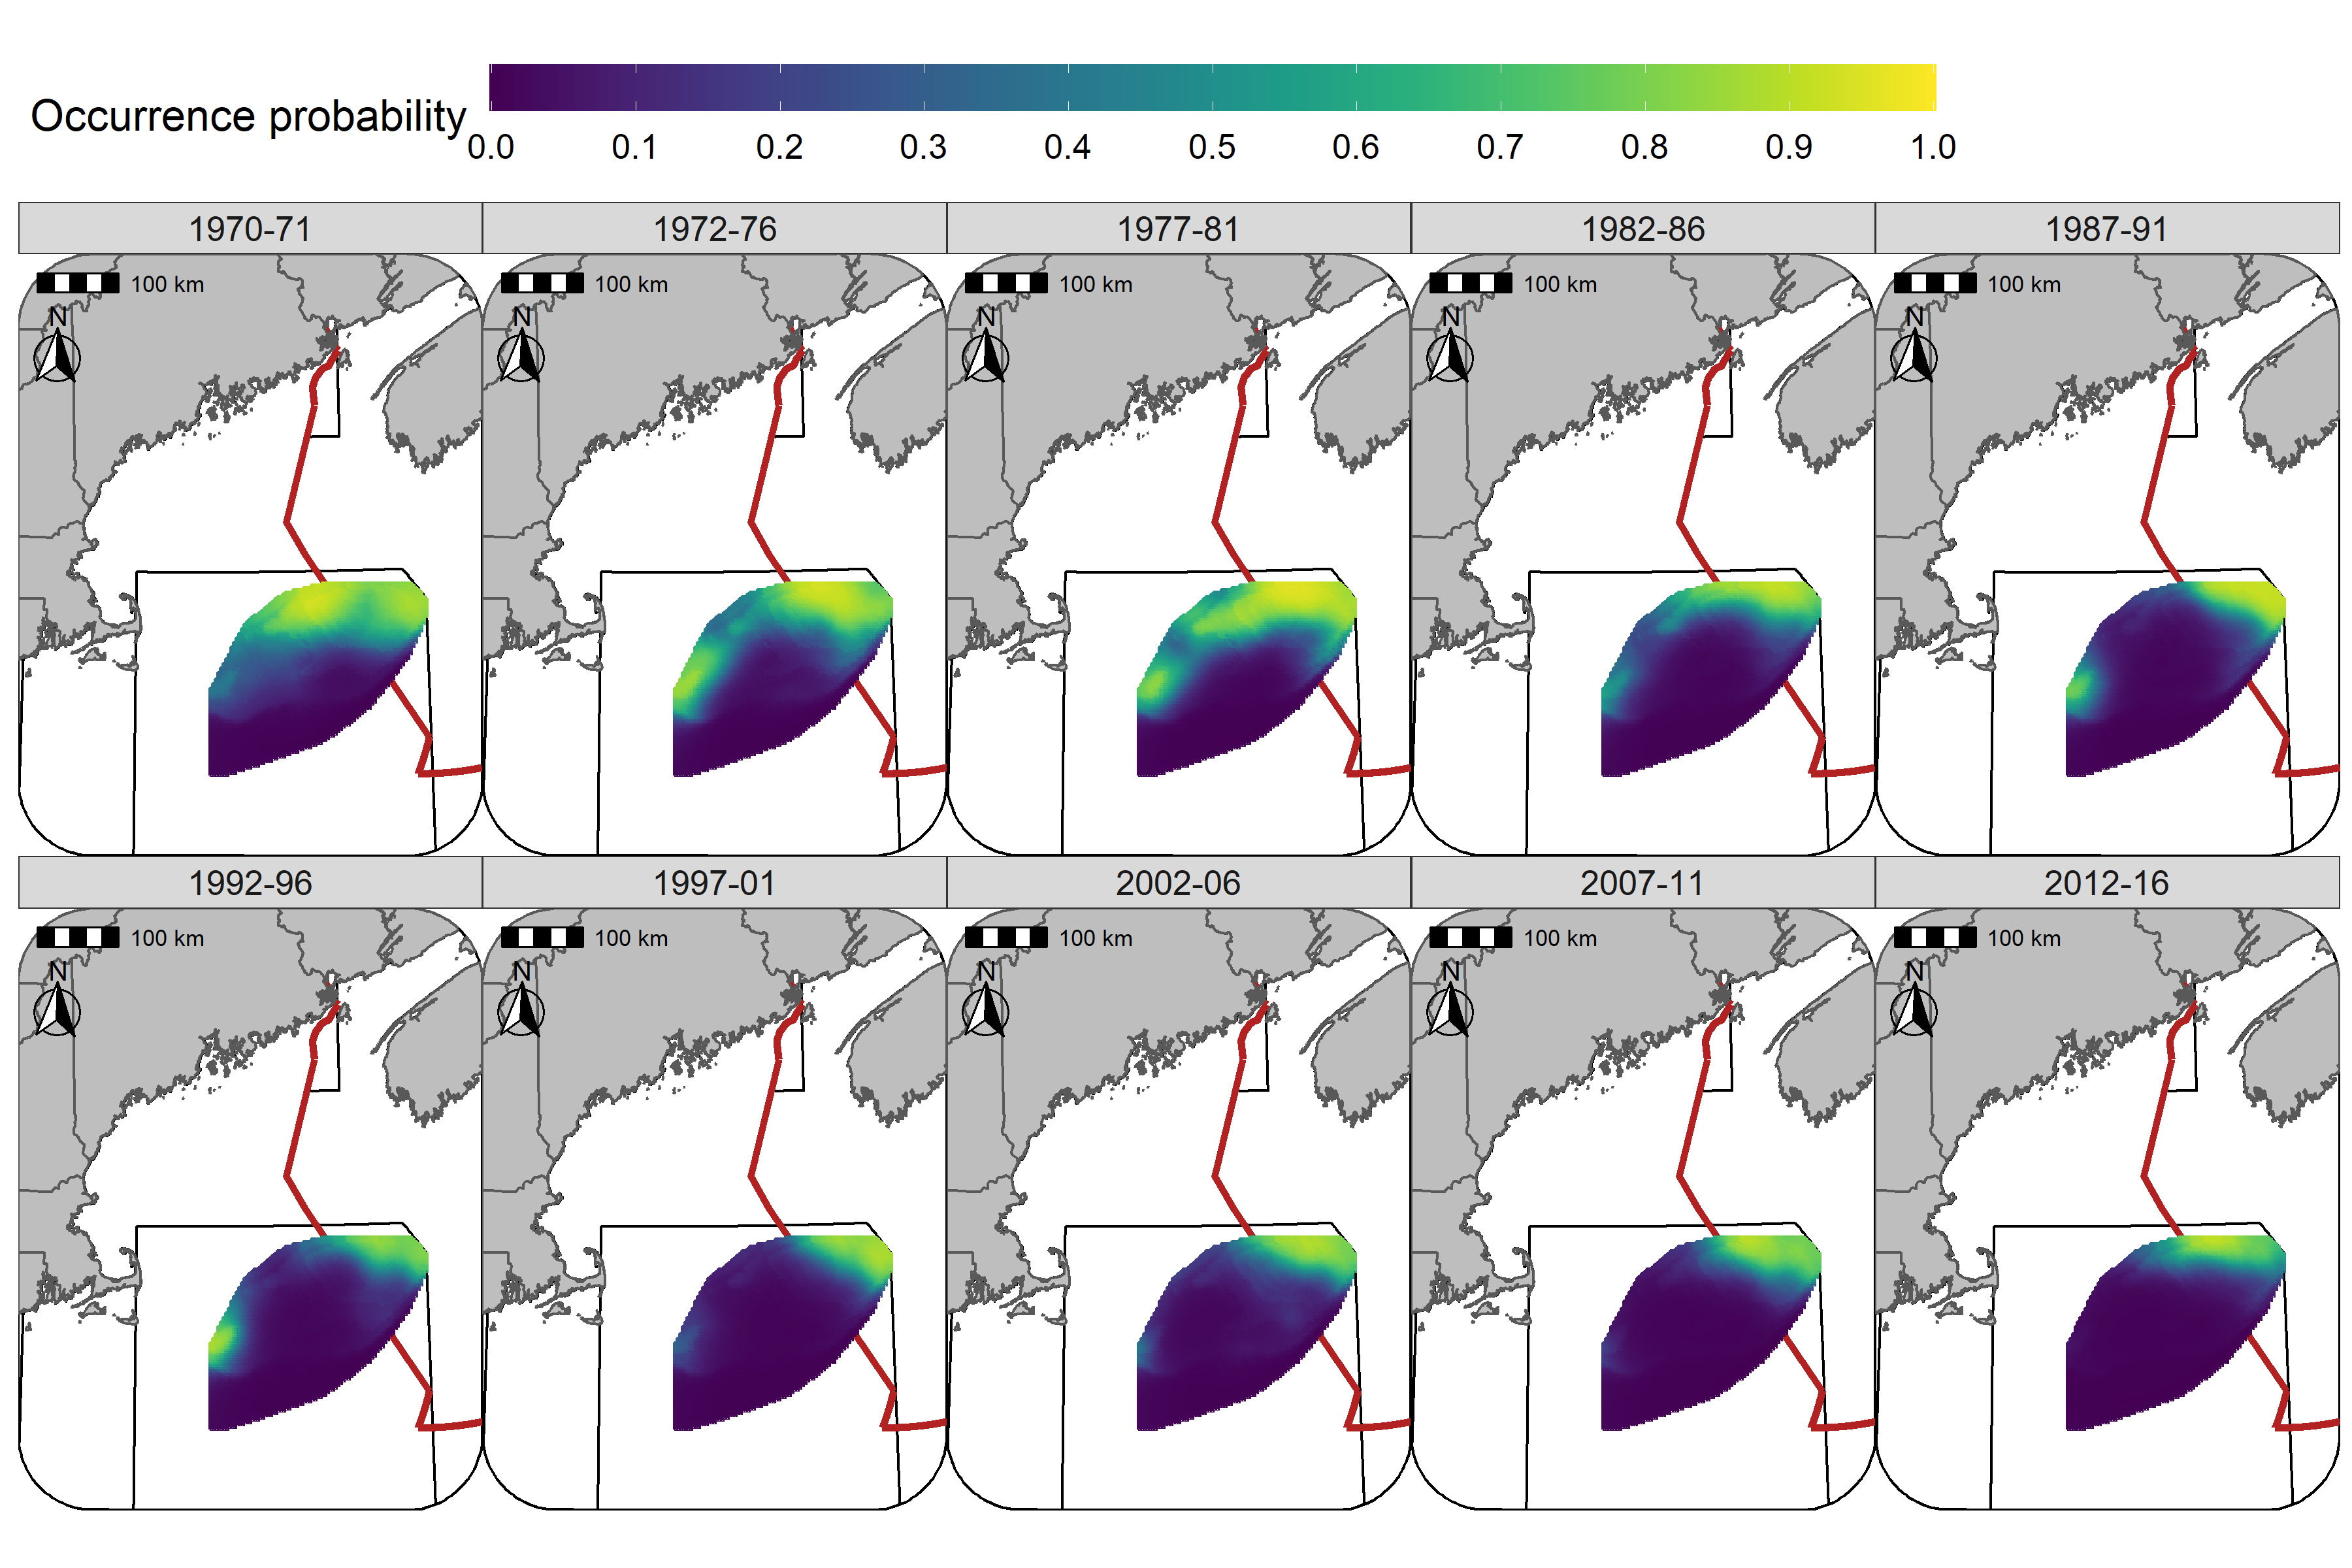
\includegraphics[width=1\linewidth]{D:/Github/Paper_2_SDMs/Results/Figures/pf_fall_cod} 

}

\caption{Predicted occurrence probability for Atlantic Cod  in each era during the Fall (NMFS-fall survey) using the SST + Depth model and 5 year random field.}\label{fig:pf-fall-cod}
\end{figure}

\newpage
\begin{figure}[htb]

{\centering 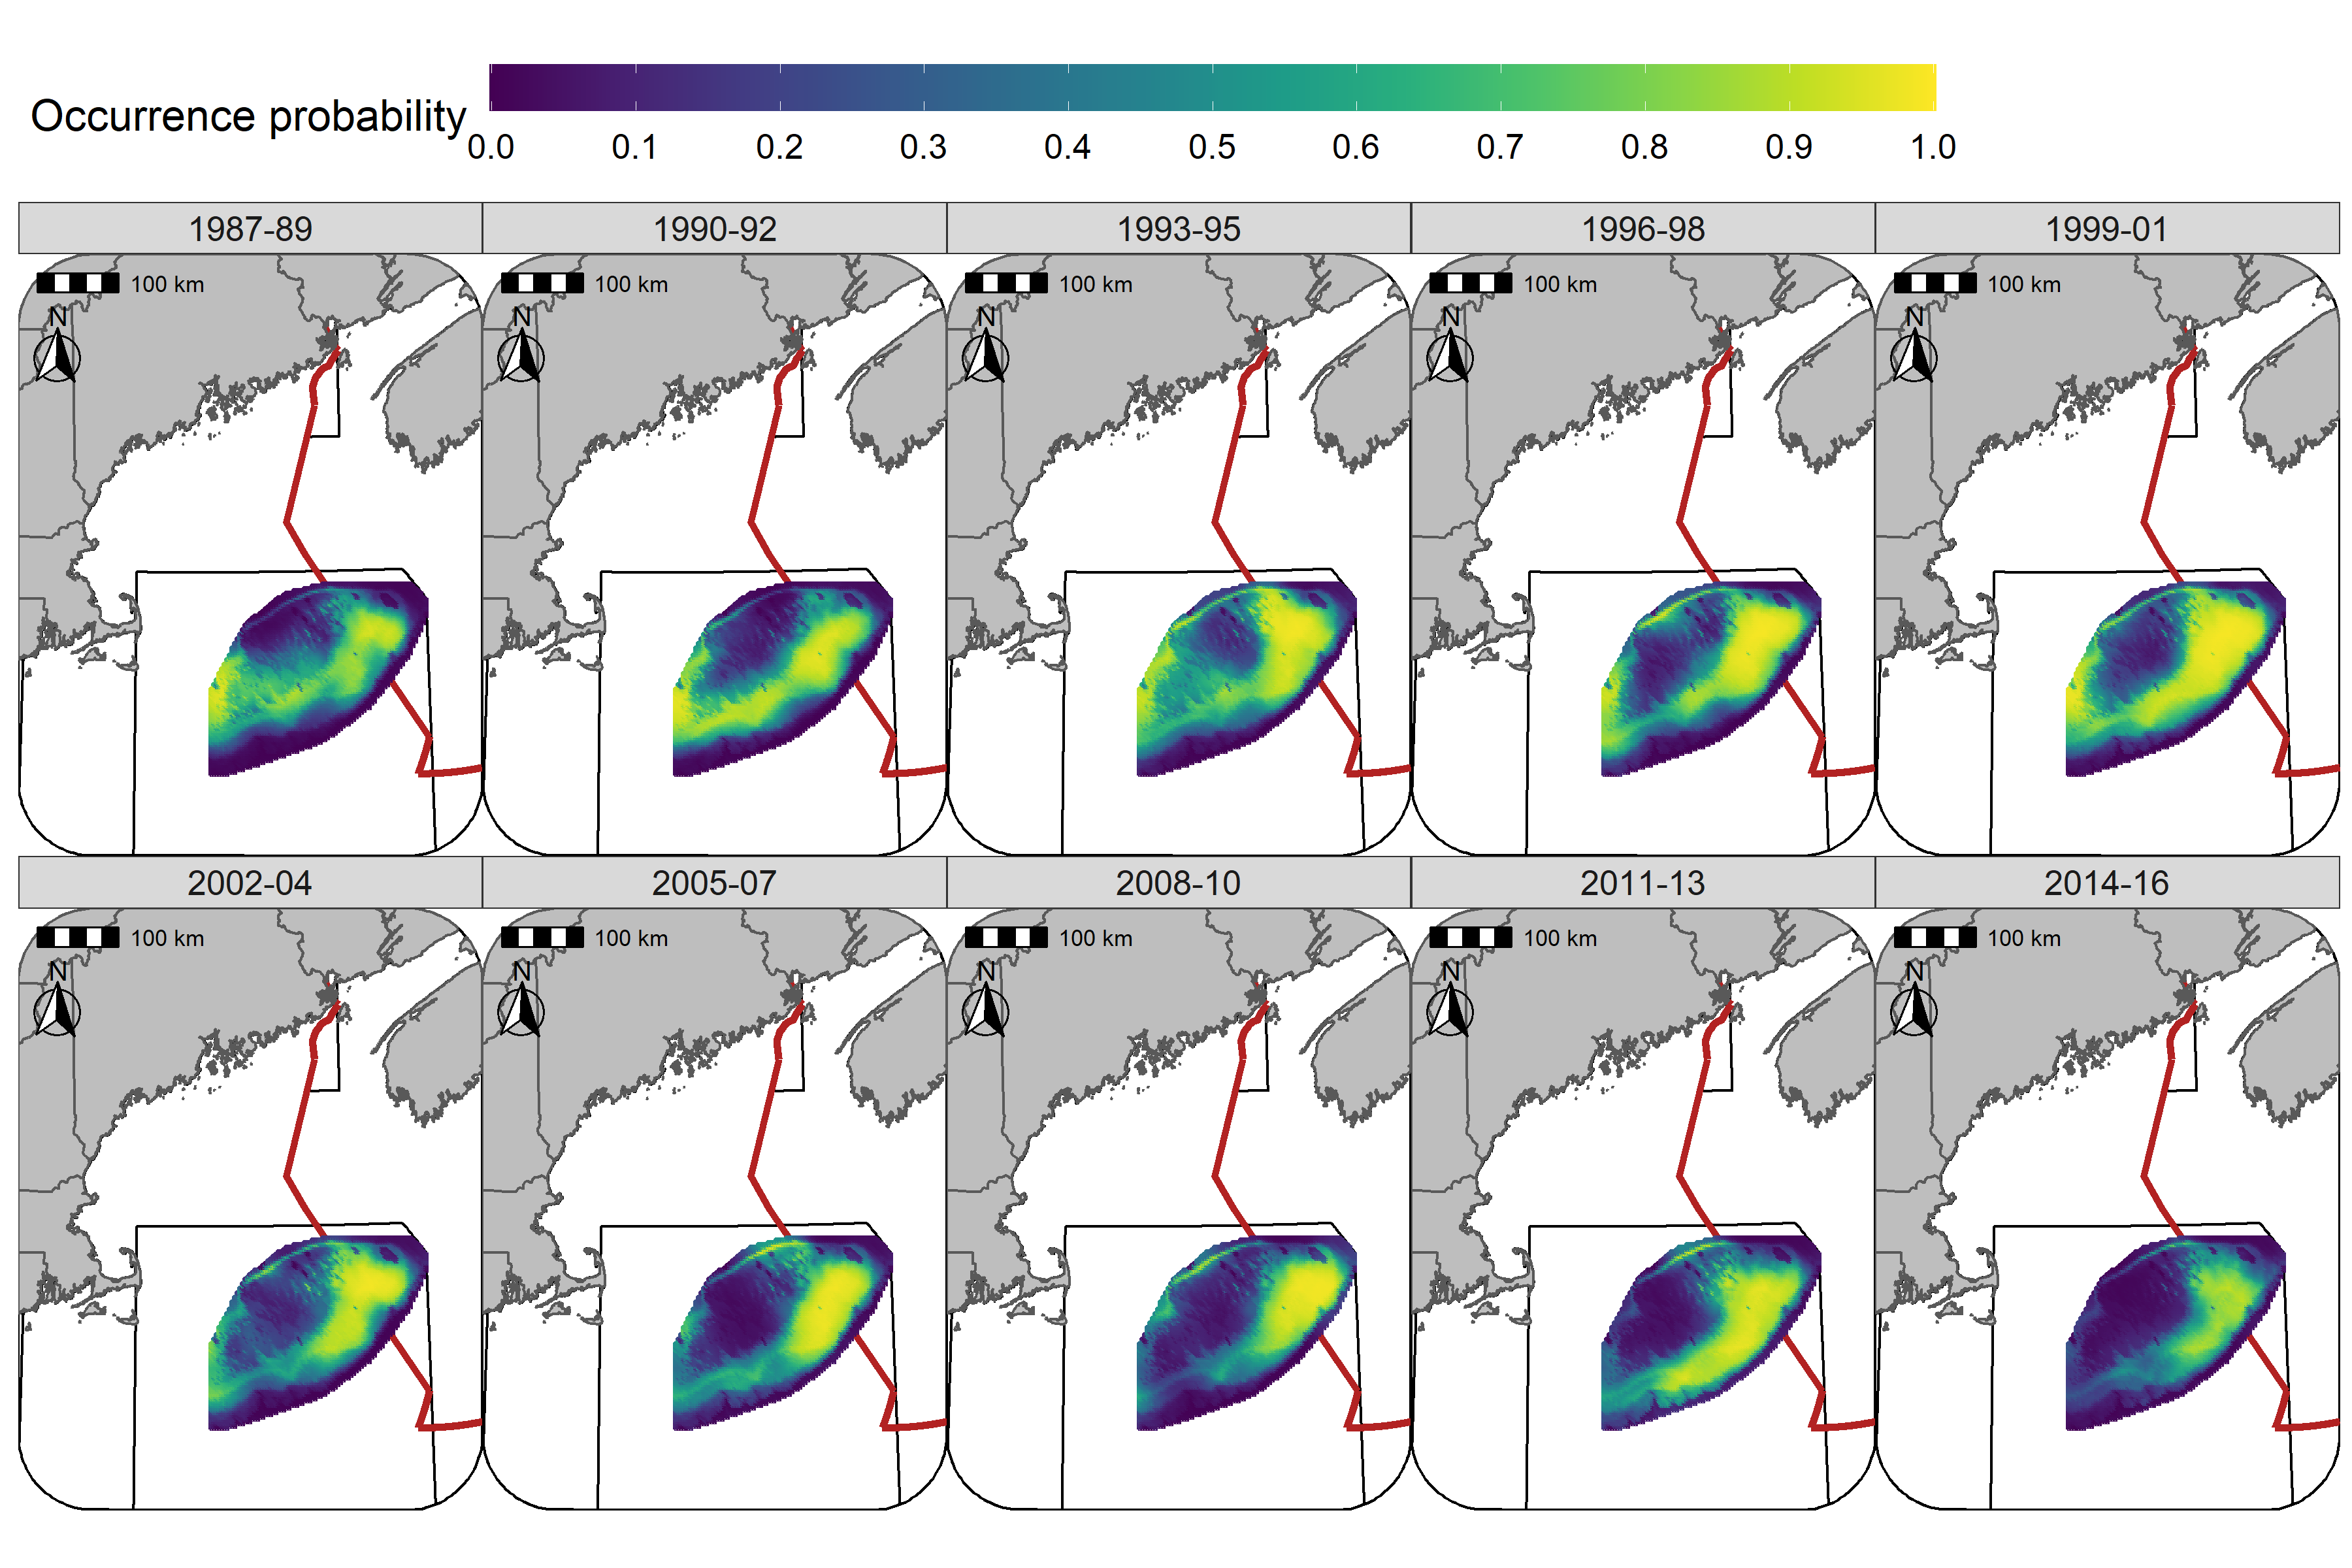
\includegraphics[width=1\linewidth]{D:/Github/Paper_2_SDMs/Results/Figures/pf_winter_yt} 

}

\caption{Predicted occurrence probability for Yellowtail Flounder in each era during the Winter (RV survey) using the SST + Depth +Sed model and 3 year random field.}\label{fig:pf-winter-yt}
\end{figure}

\newpage
\begin{figure}[htb]

{\centering 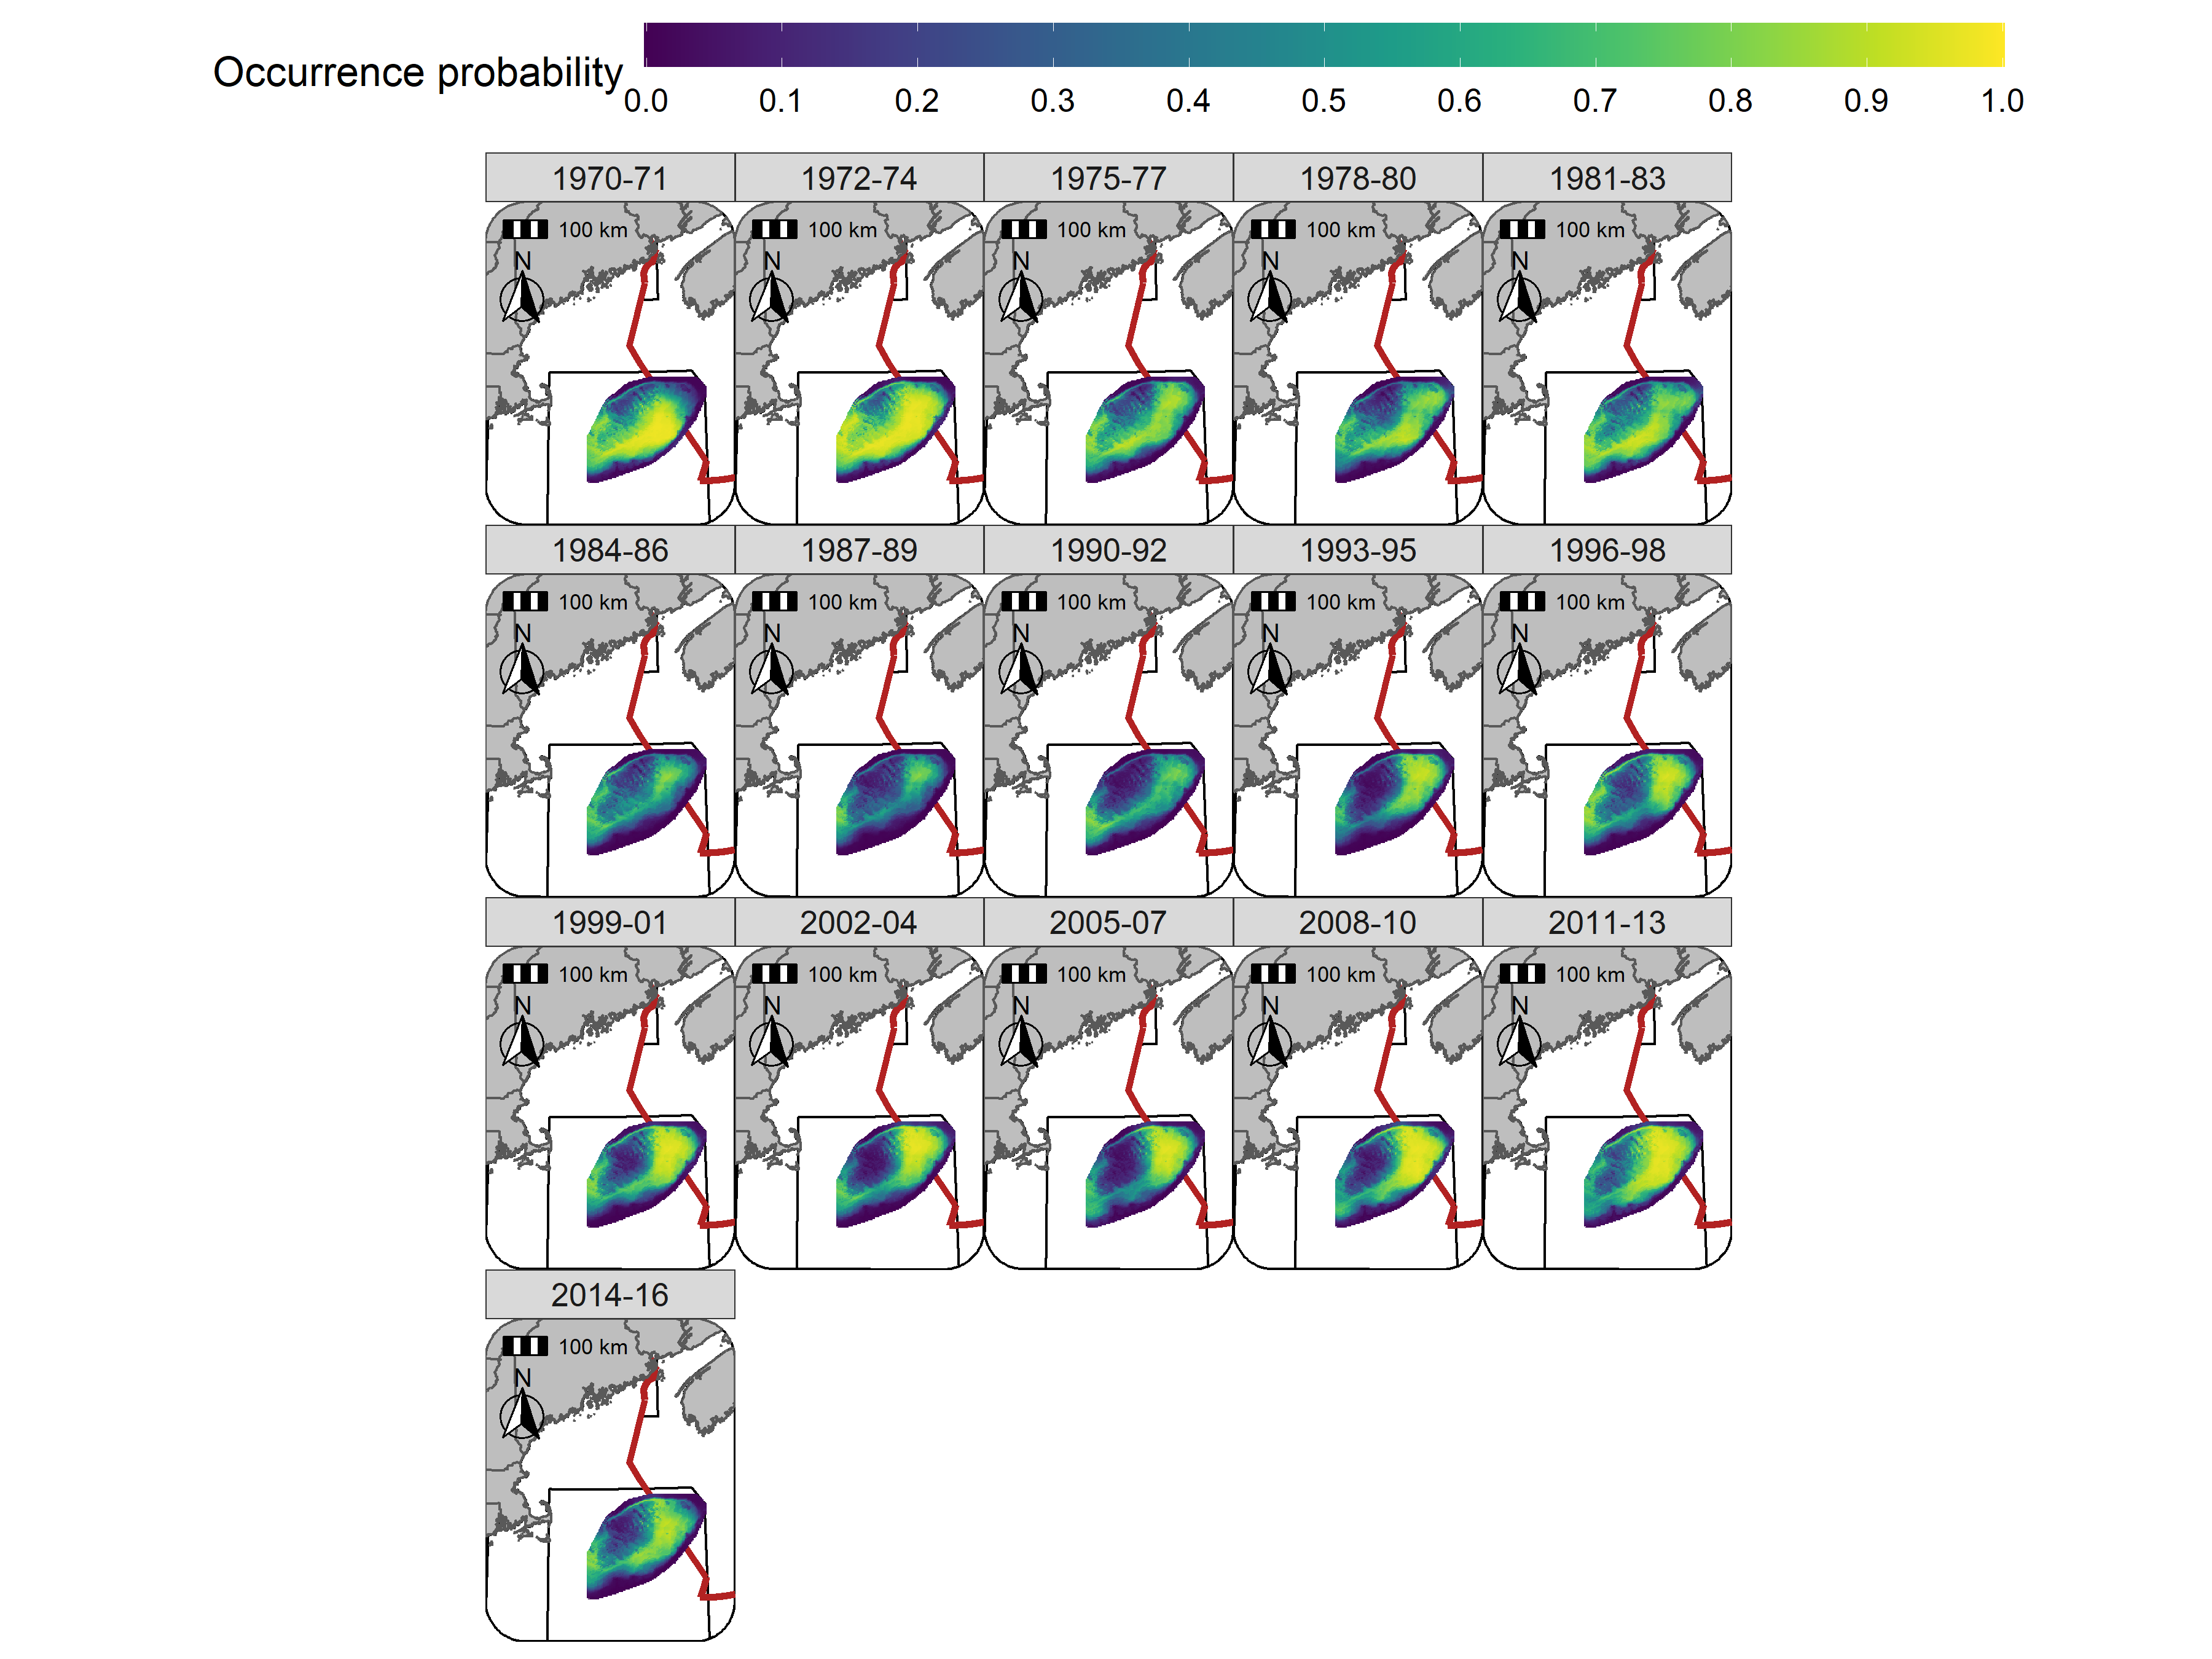
\includegraphics[width=1\linewidth]{D:/Github/Paper_2_SDMs/Results/Figures/pf_spring_yt} 

}

\caption{Predicted occurrence probability for Yellowtail Flounder in each era during the Spring (NMFS-spring survey) using the SST + Depth + Sed  model and 3 year random field.}\label{fig:pf-spring-yt}
\end{figure}

\newpage
\begin{figure}[htb]

{\centering 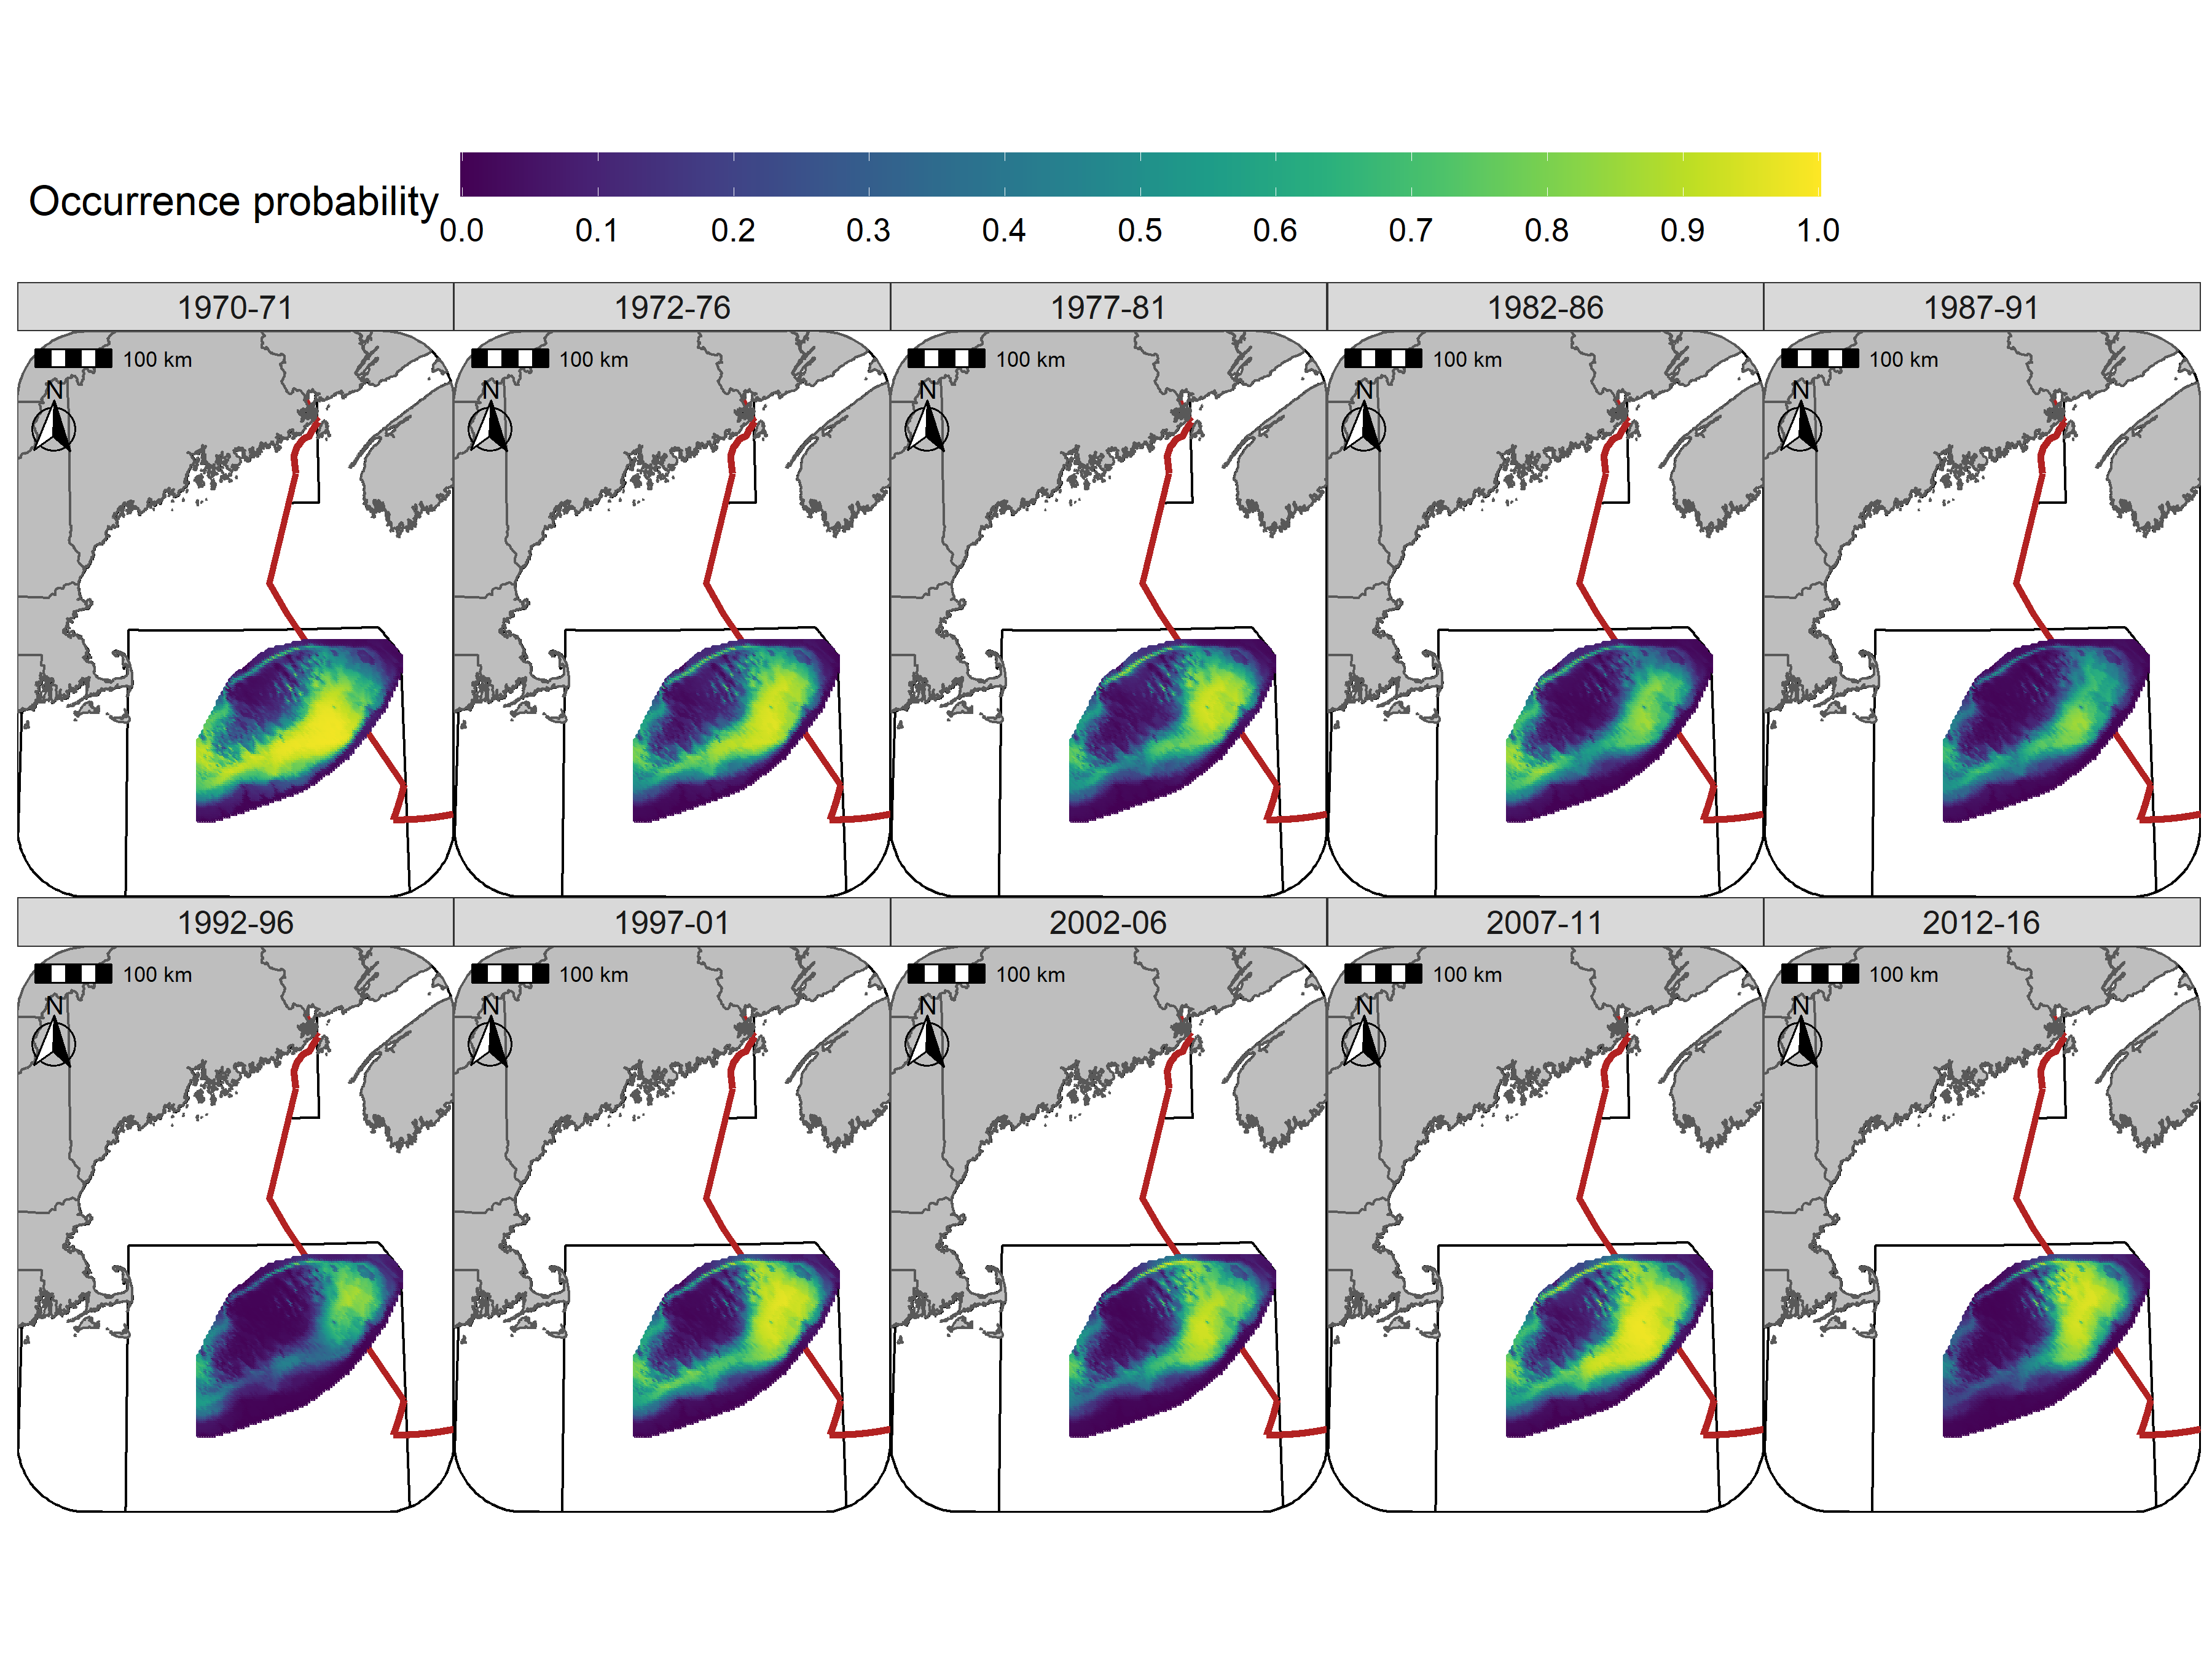
\includegraphics[width=1\linewidth]{D:/Github/Paper_2_SDMs/Results/Figures/pf_fall_yt} 

}

\caption{Predicted occurrence probability for Yellowtail Flounder in each era during the Fall (NMFS-fall survey) using the SST + Depth + Sed model and 5 year random field.}\label{fig:pf-fall-yt}
\end{figure}

\newpage

\begin{figure}[htb]

{\centering 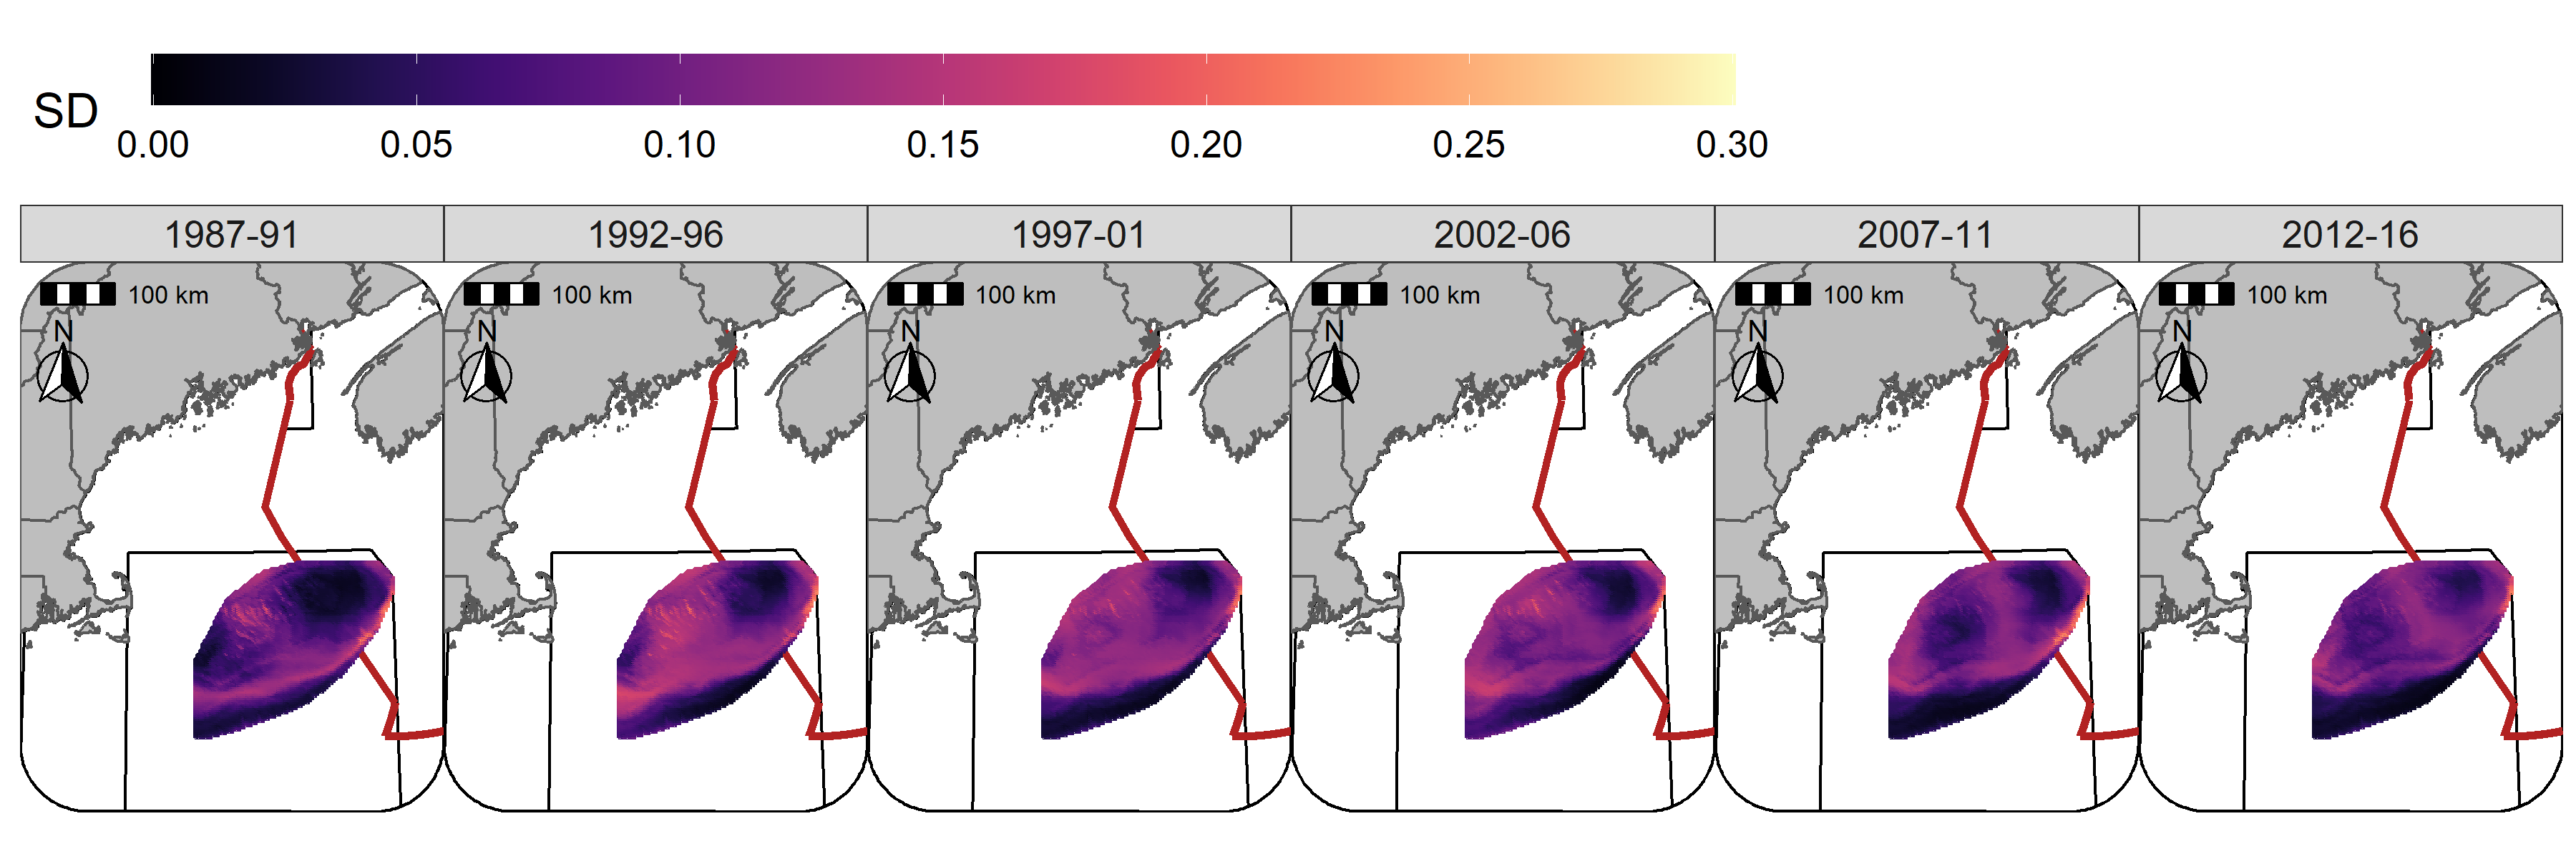
\includegraphics[width=1\linewidth]{D:/Github/Paper_2_SDMs/Results/Figures/pf_winter_cod_sd} 

}

\caption{Standard deviation (logit scale) of predicted occurrence probability for Atlantic Cod  in each era during the Winter (RV survey) using the SST + Depth model and 5 year random field.}\label{fig:pf-winter-cod-sd}
\end{figure}

\newpage
\begin{figure}[htb]

{\centering 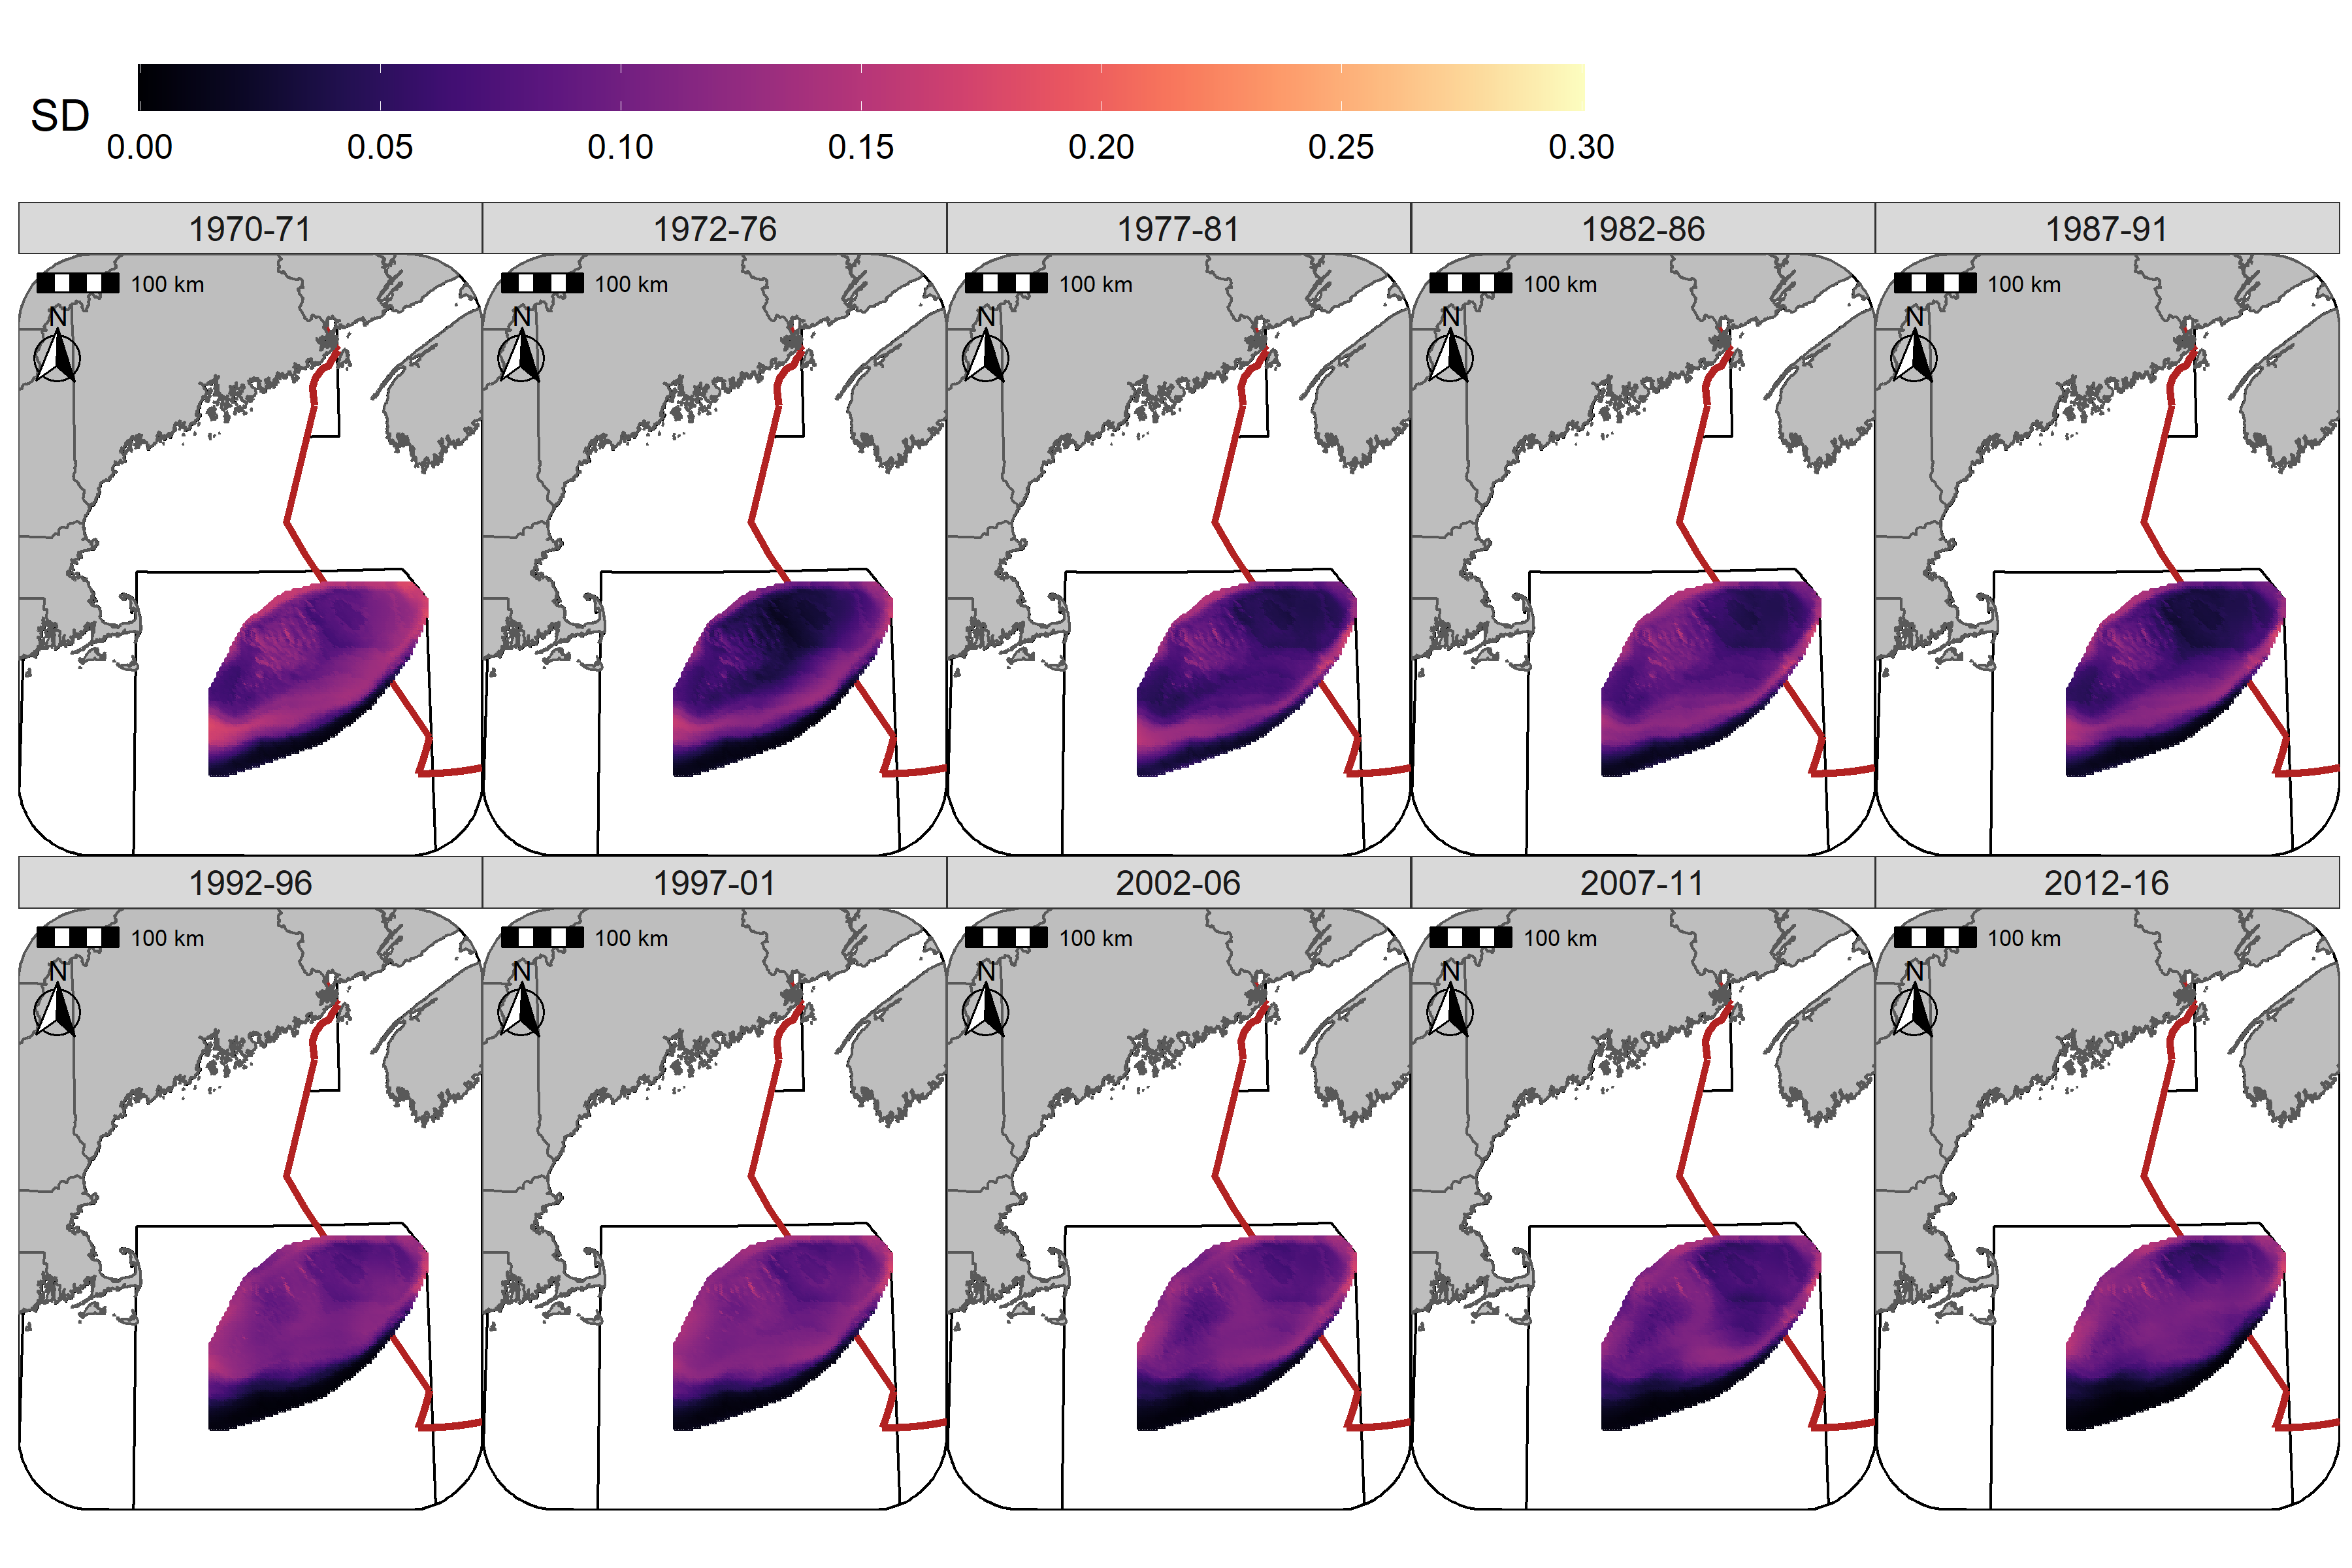
\includegraphics[width=1\linewidth]{D:/Github/Paper_2_SDMs/Results/Figures/pf_spring_cod_sd} 

}

\caption{Standard deviation (logit scale) of predicted occurrence probability for Atlantic Cod  in each era during the Spring (NMFS-spring survey) using the SST + Depth model and 5 year random field.}\label{fig:pf-spring-cod-sd}
\end{figure}

\newpage
\begin{figure}[htb]

{\centering 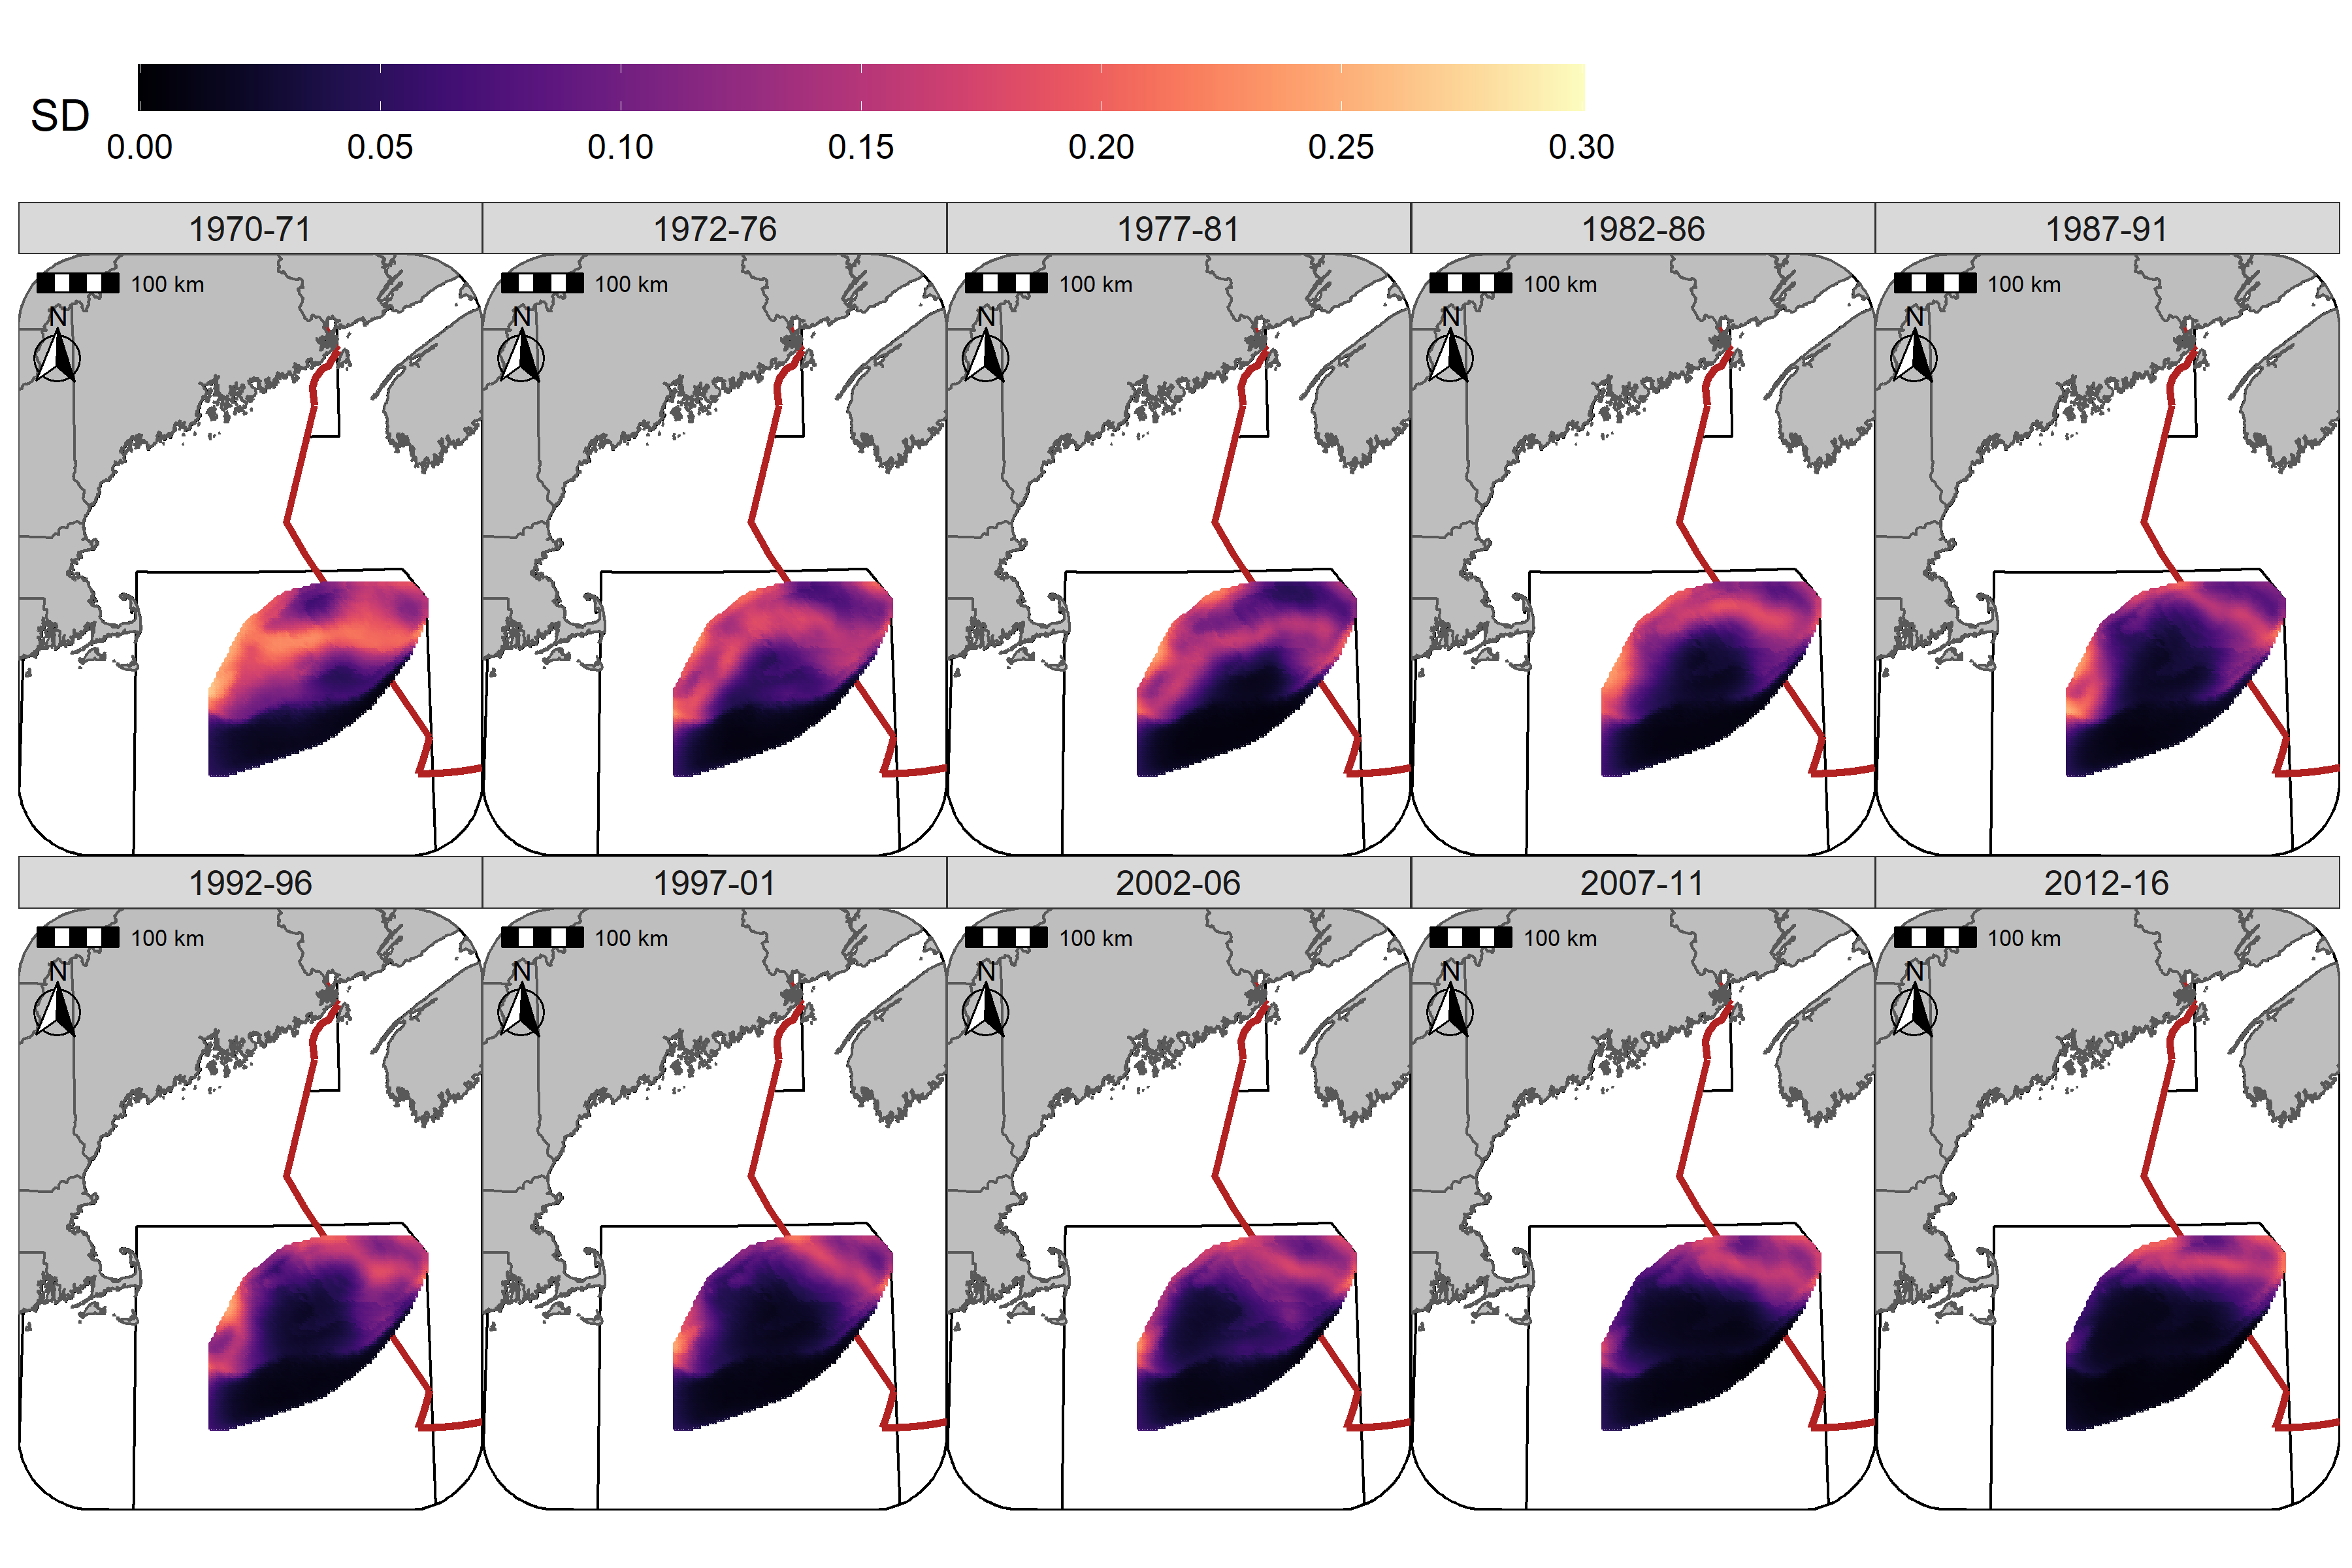
\includegraphics[width=1\linewidth]{D:/Github/Paper_2_SDMs/Results/Figures/pf_fall_cod_sd} 

}

\caption{Standard deviation (logit scale) of predicted occurrence probability for Atlantic Cod  in each era during the Fall (NMFS-fall survey) using the SST + Depth model and 5 year random field.}\label{fig:pf-fall-cod-sd}
\end{figure}

\newpage
\begin{figure}[htb]

{\centering 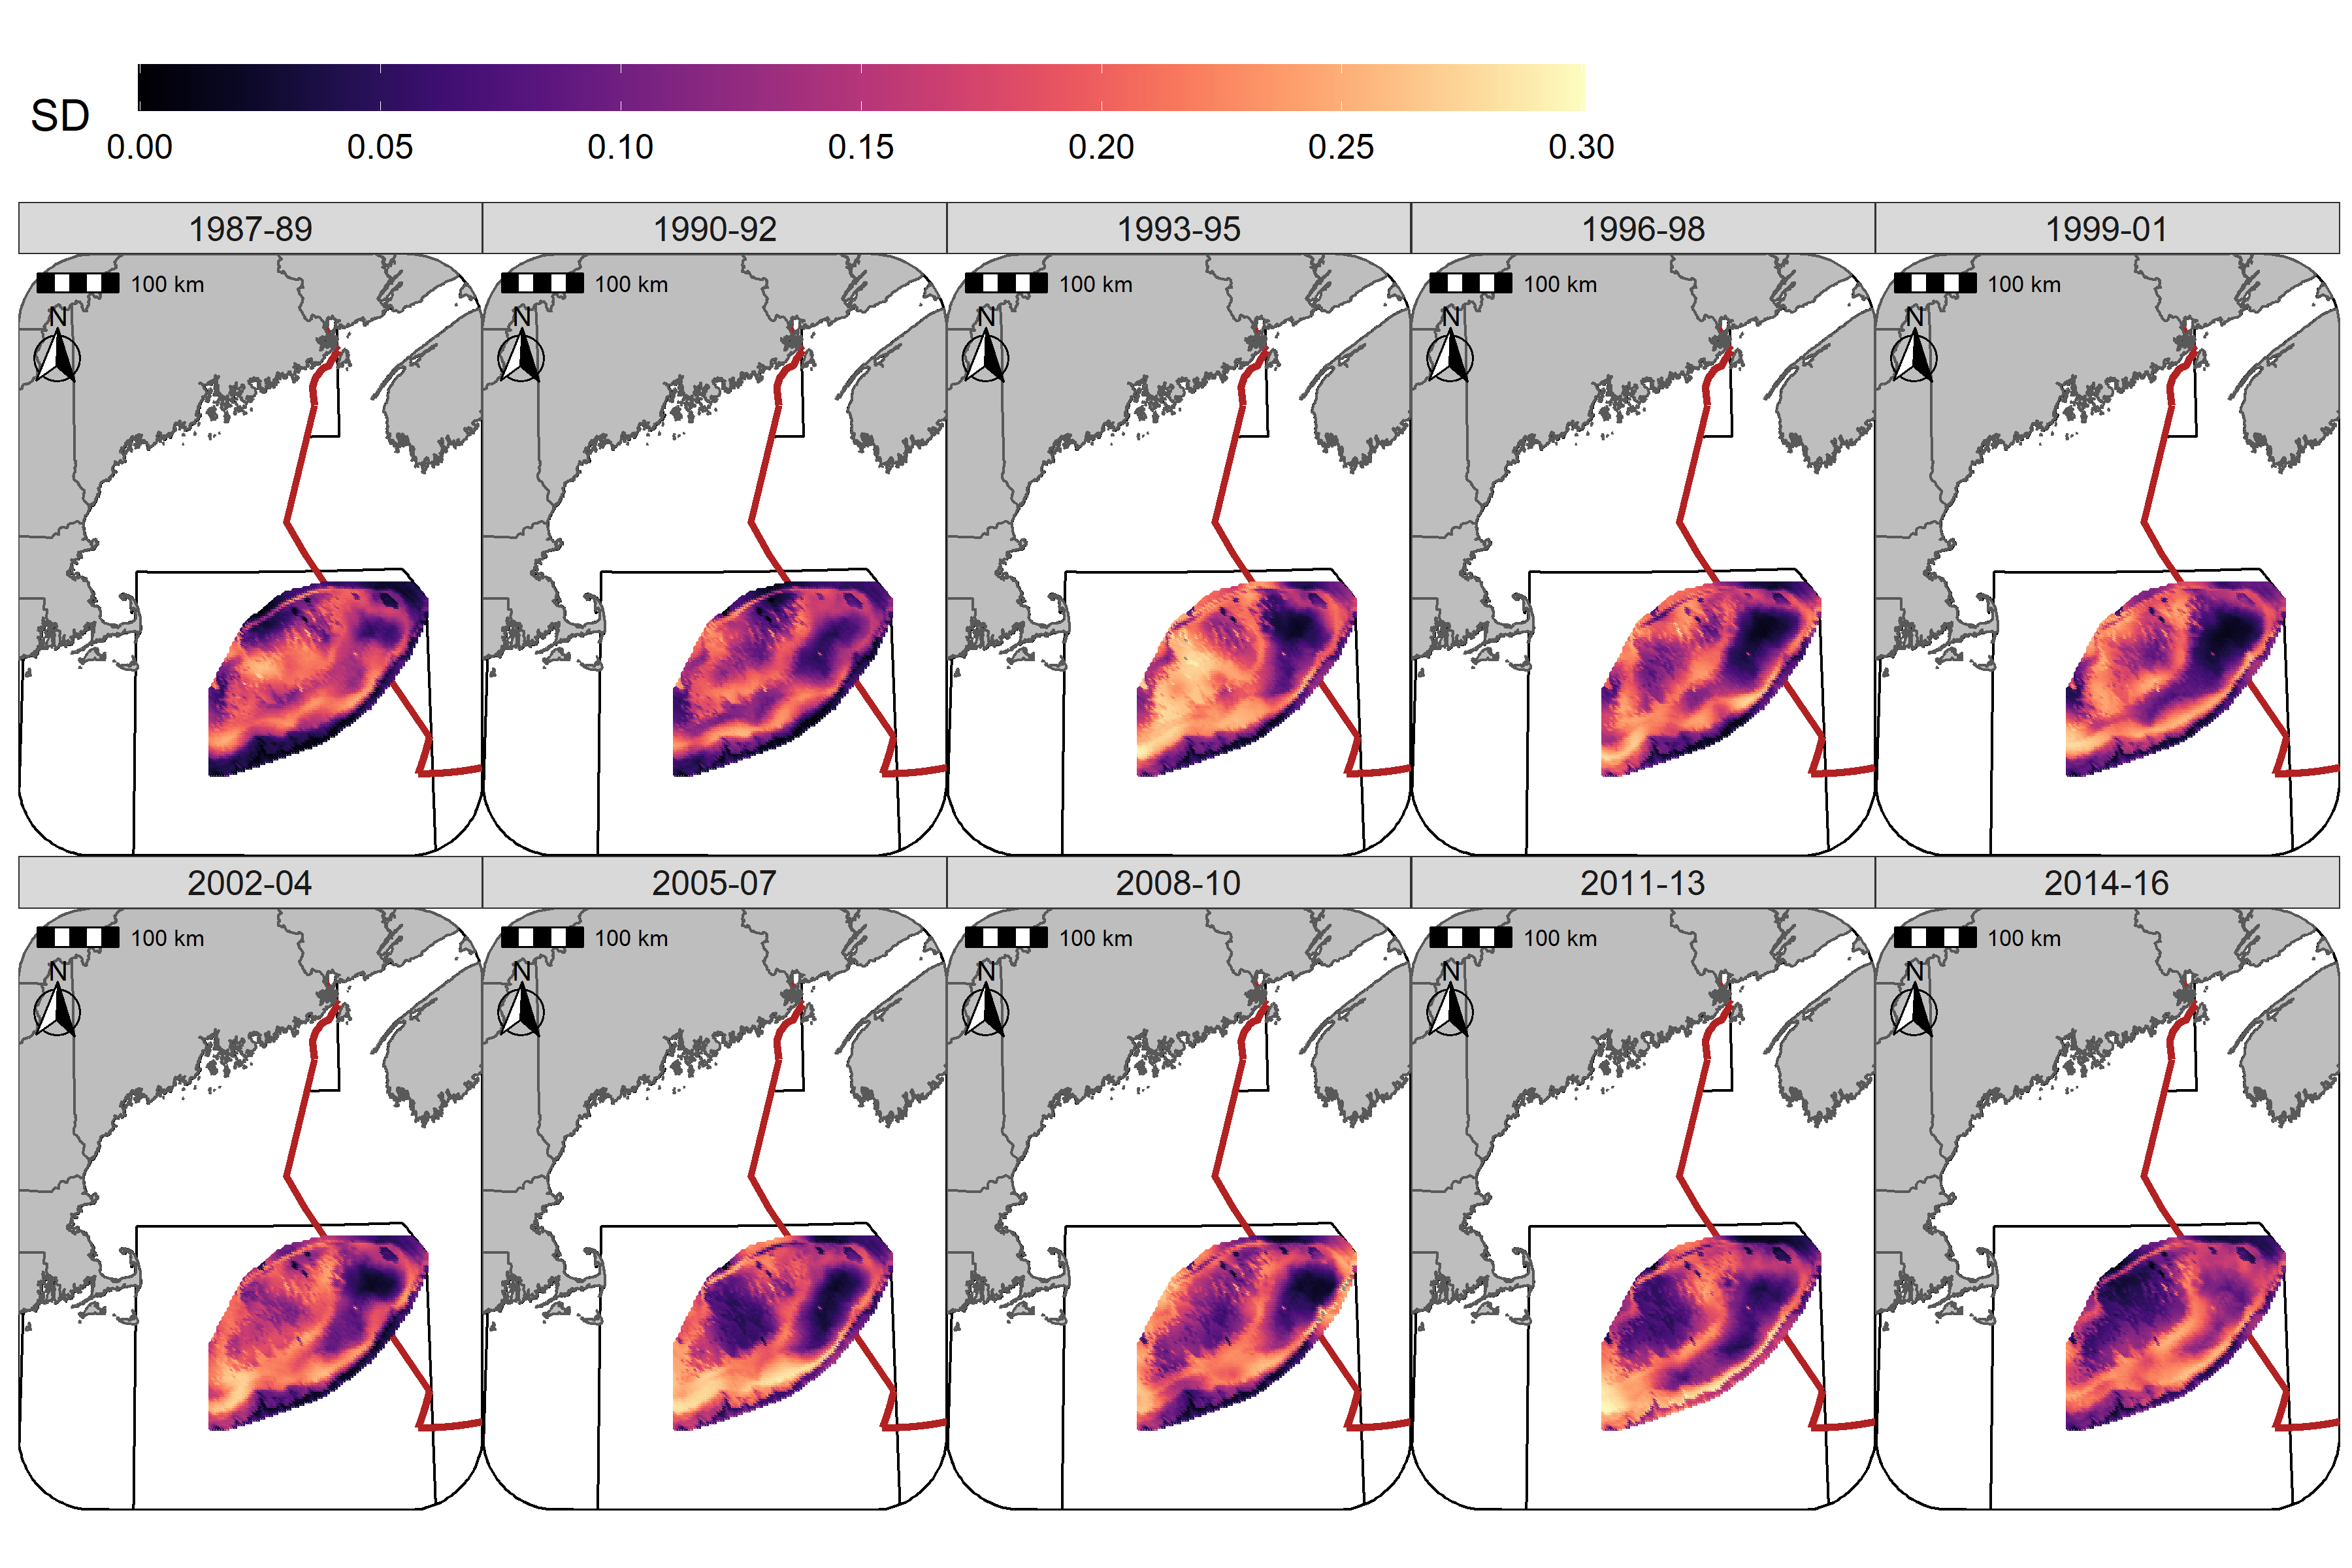
\includegraphics[width=1\linewidth]{D:/Github/Paper_2_SDMs/Results/Figures/pf_winter_yt_sd} 

}

\caption{Standard deviation (logit scale) of predicted occurrence probability for Yellowtail Flounder in each era during the Winter (RV survey) using the SST + Depth + Sed  model and 3 year random field.}\label{fig:pf-winter-yt-sd}
\end{figure}

\newpage

\begin{figure}[htb]

{\centering 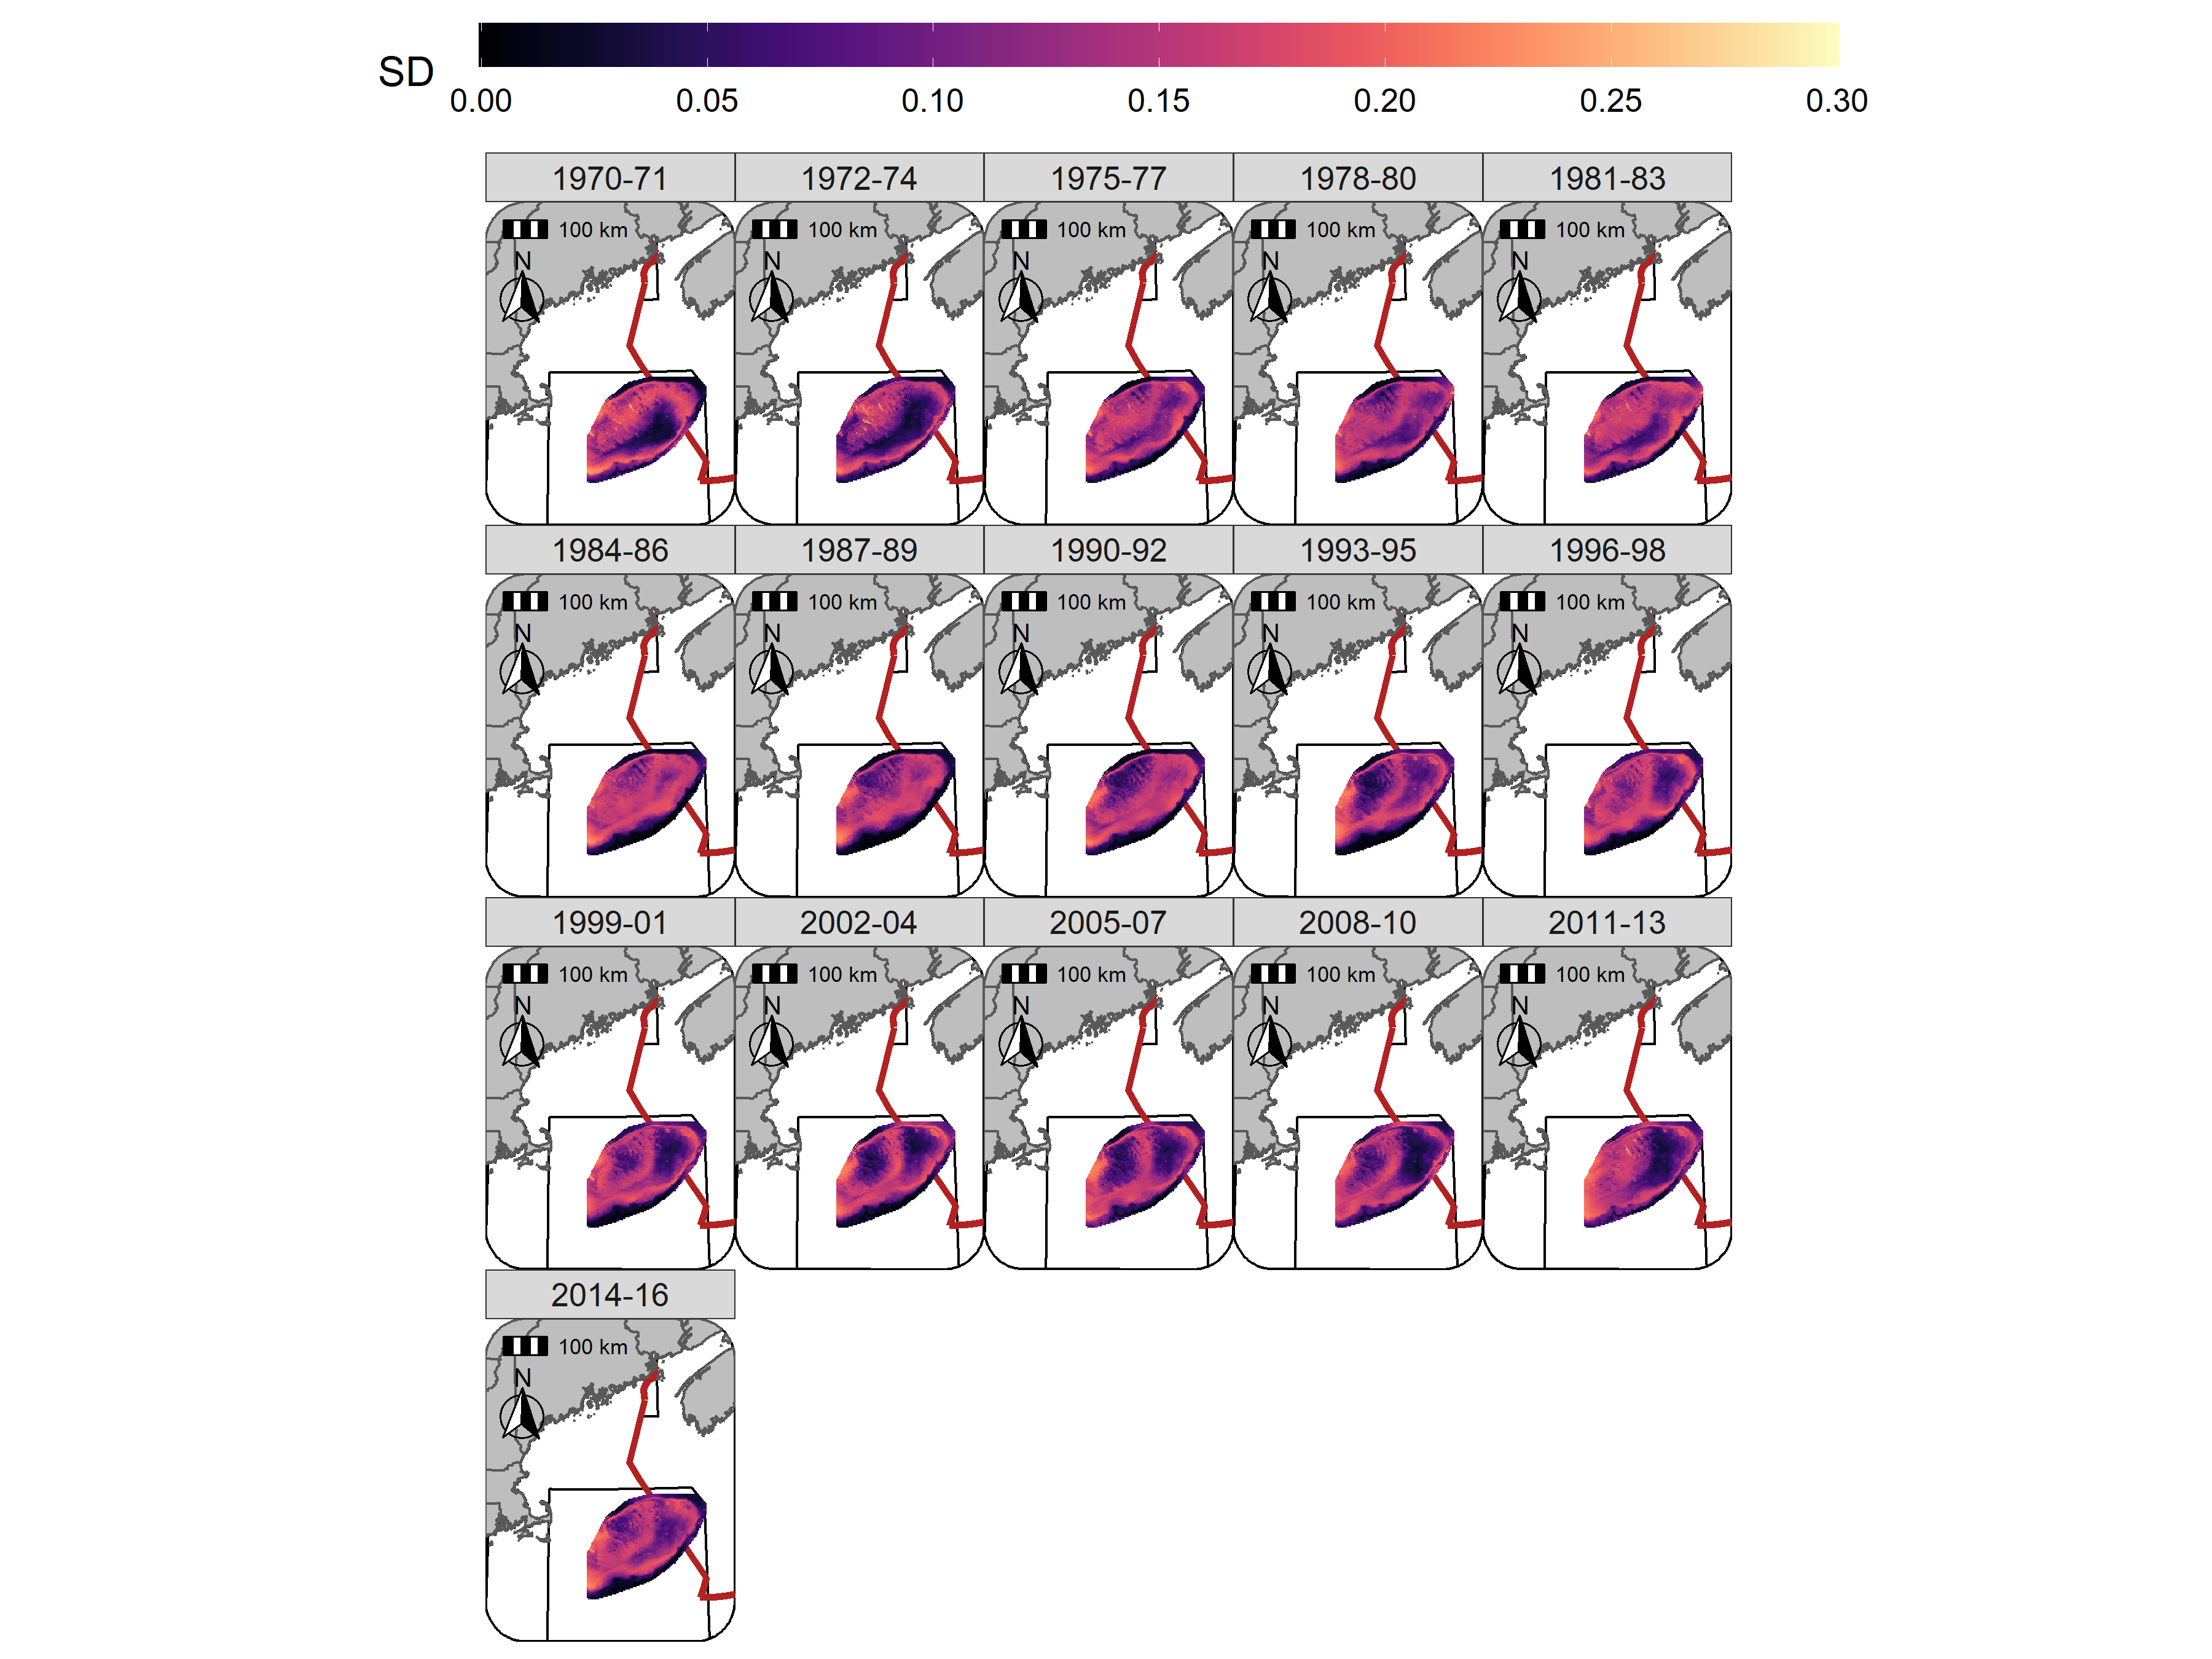
\includegraphics[width=1\linewidth]{D:/Github/Paper_2_SDMs/Results/Figures/pf_spring_yt_sd} 

}

\caption{Standard deviation (logit scale) of predicted occurrence probability for Yellowtail Flounder in each era during the Spring (NMFS-spring survey) using the  SST + Depth + Sed  model and 3 year random field.}\label{fig:pf-spring-yt-sd}
\end{figure}

\newpage
\begin{figure}[htb]

{\centering 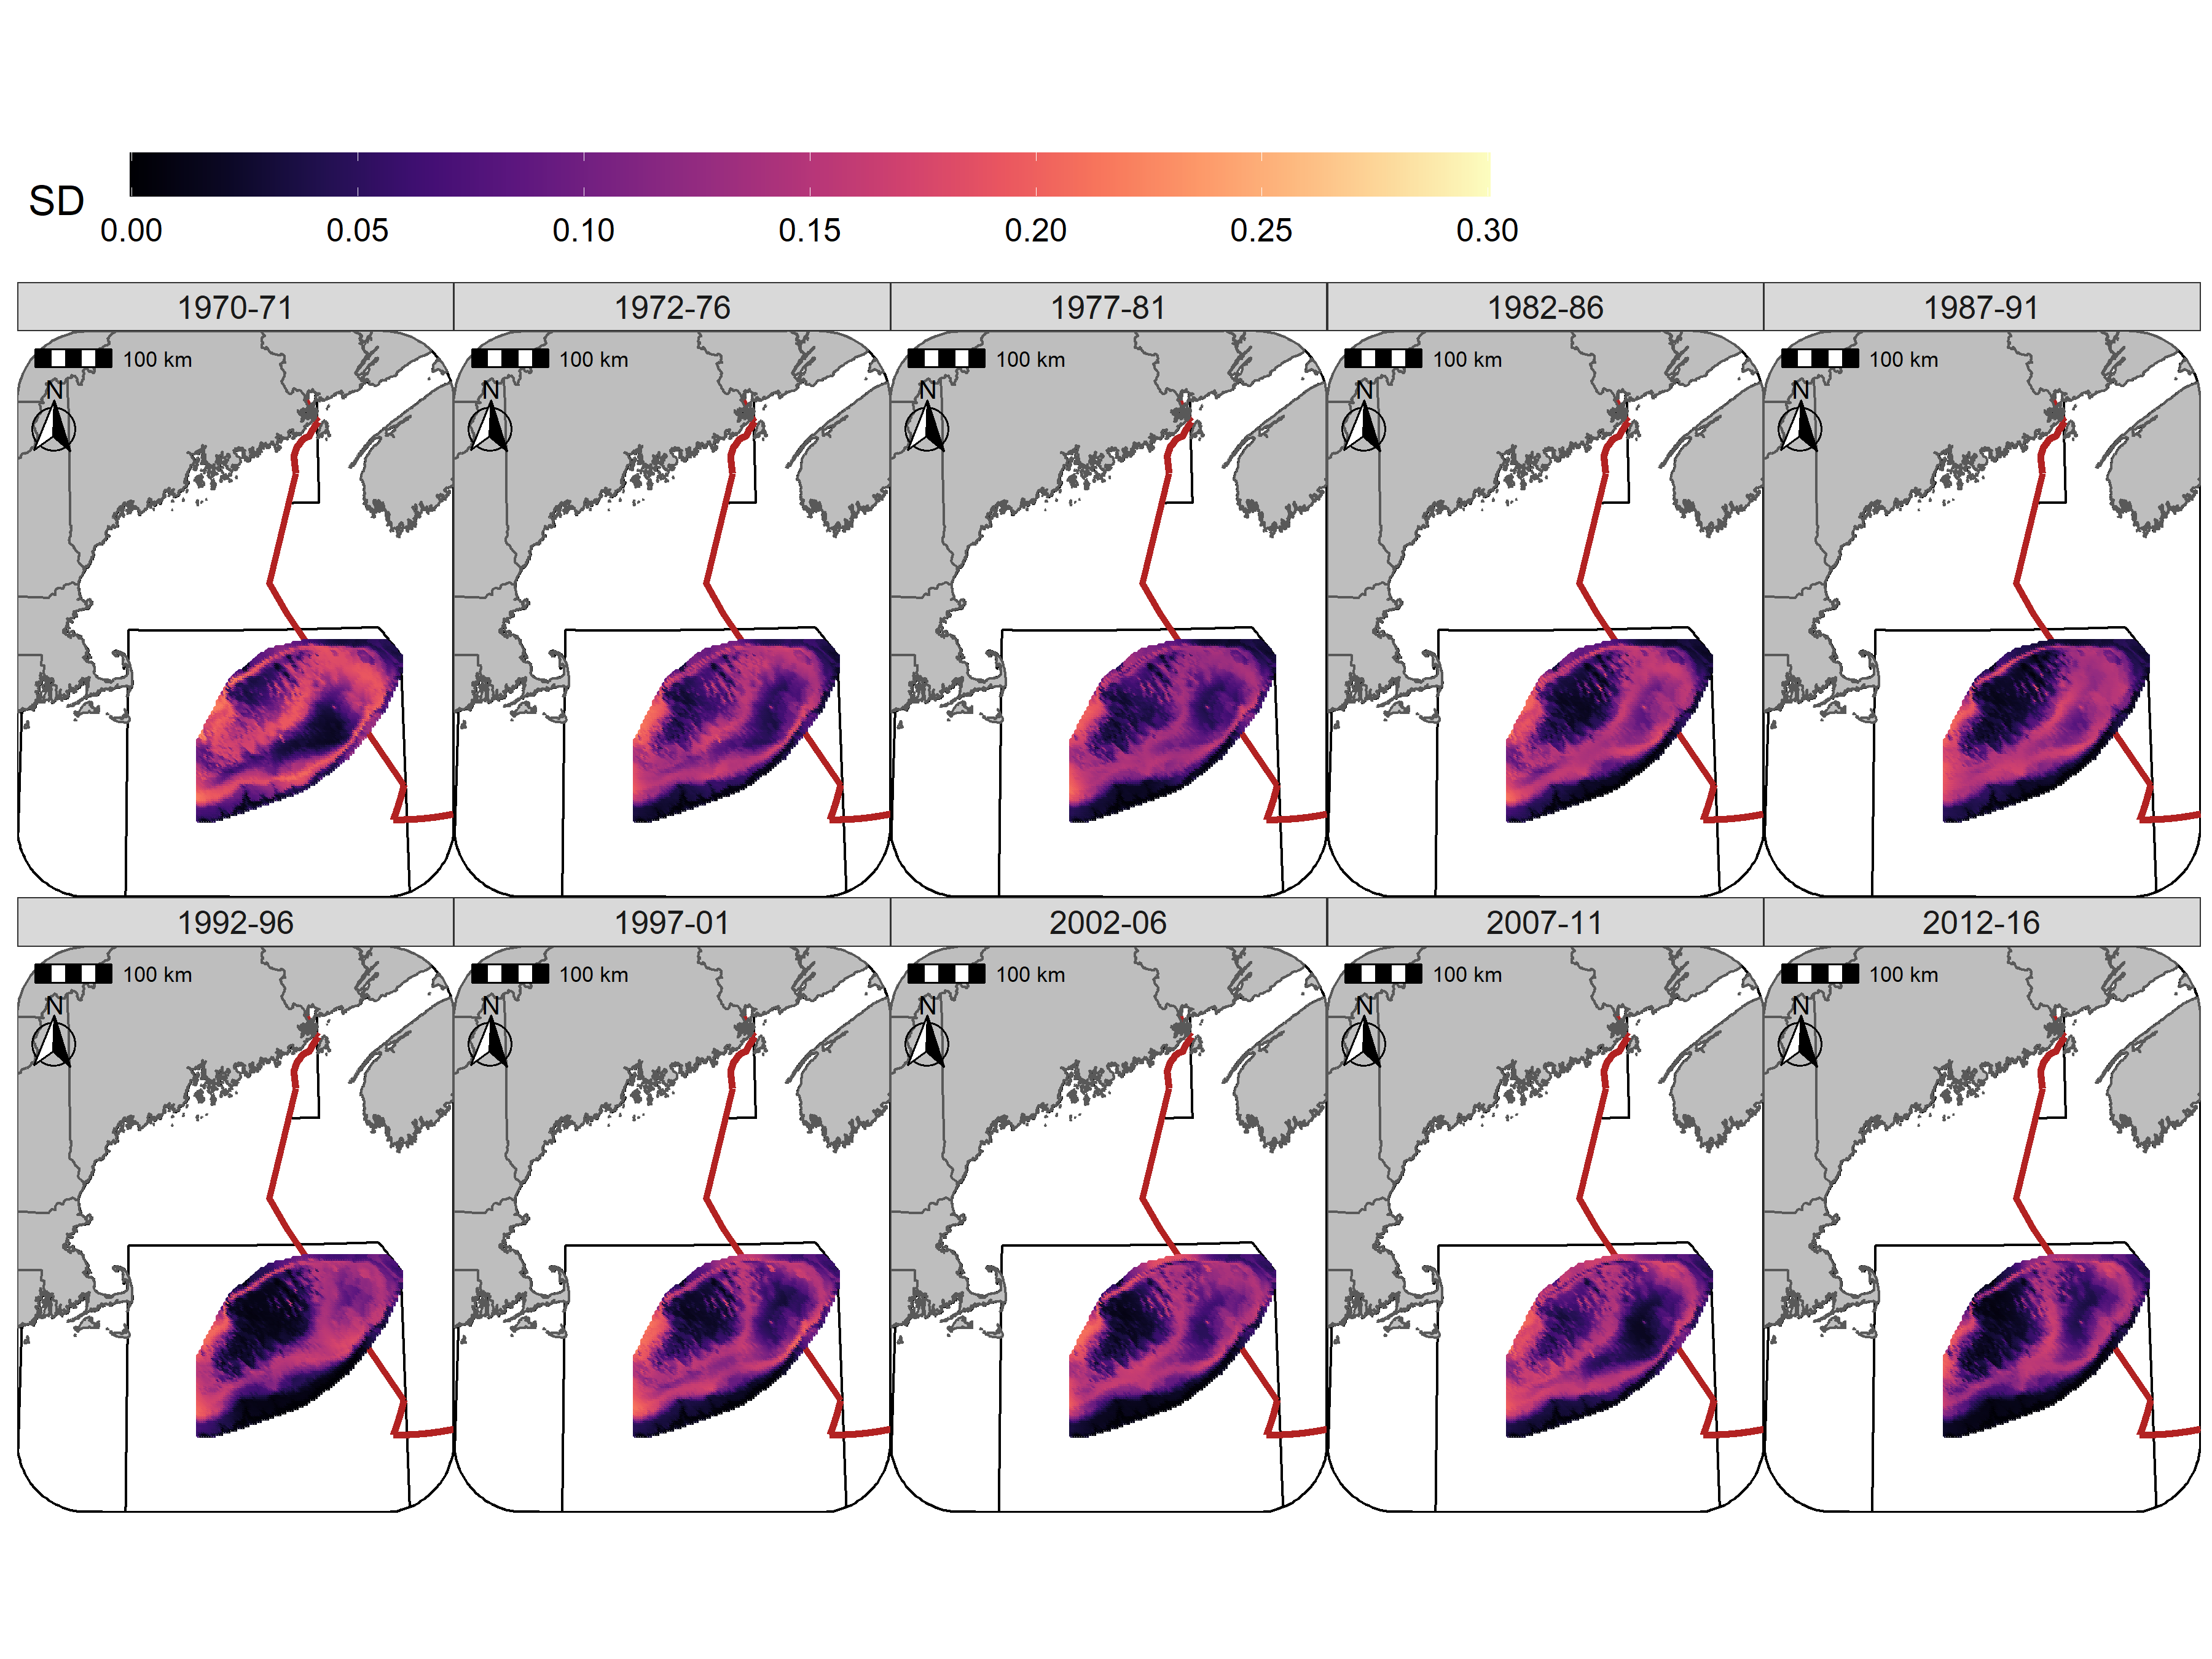
\includegraphics[width=1\linewidth]{D:/Github/Paper_2_SDMs/Results/Figures/pf_fall_yt_sd} 

}

\caption{Standard deviation (logit scale) of predicted occurrence probability for Yellowtail Flounder in each era during the Fall (NMFS-fall survey) using the SST + Depth + Sed  model and 5 year random field.}\label{fig:pf-fall-yt-sd}
\end{figure}
\end{landscape}

\clearpage

\hypertarget{random-fields}{%
\subsection{Random fields}\label{random-fields}}

The 5-year random fields for Atlantic Cod in the Winter and Spring are seasonally consistent through time, with lower effect sizes observed in both seasons starting in 1992 and the largest declines in the effect size observed in the southern and western portions of GB (Figures \ref{fig:rf-winter-cod} - \ref{fig:rf-spring-cod}). In the Fall the higher effect sizes were generally observed towards the north and in Canadian waters, with larger declines in the random field effect size towards the west over the study period (Figure \ref{fig:rf-fall-cod}).

The Yellowtail Flounder random field patterns were similar in the Winter and Spring while the random field effect sizes were somewhat smaller during the Fall (Figures \ref{fig:rf-winter-yt} - \ref{fig:rf-fall-yt}). The effect size of the random fields, in all seasons, were lower throughout the later half of the 1980s and the early 1990s. The highest effect size of the random fields were observed in the 1970s and in the 2000s. Since the mid-1970s an area straddling the Canadian-U.S. border has been consistently identified as an area where the Yellowtail Flounder effect size of the random field is elevated (Figures \ref{fig:rf-winter-yt} - \ref{fig:rf-fall-yt}).

The standard deviation (SD) of the random fields for Atlantic Cod were also similar between seasons with the lowest SD generally observed in the north and east and highest approaching the southern flank of GB. The SD was somewhat higher in the Fall throughout the central portion of GB (Figures \ref{fig:rf-winter-cod-sd} - \ref{fig:rf-fall-cod-sd}). For Yellowtail Flounder, the SD was higher towards the southern portions of the bank with localized regions having elevated SD scattered throughout the bank in the Winter, Spring and Fall. (Figures \ref{fig:rf-winter-yt-sd} - \ref{fig:rf-fall-yt-sd}).

\begin{landscape}
\begin{figure}[htb]

{\centering 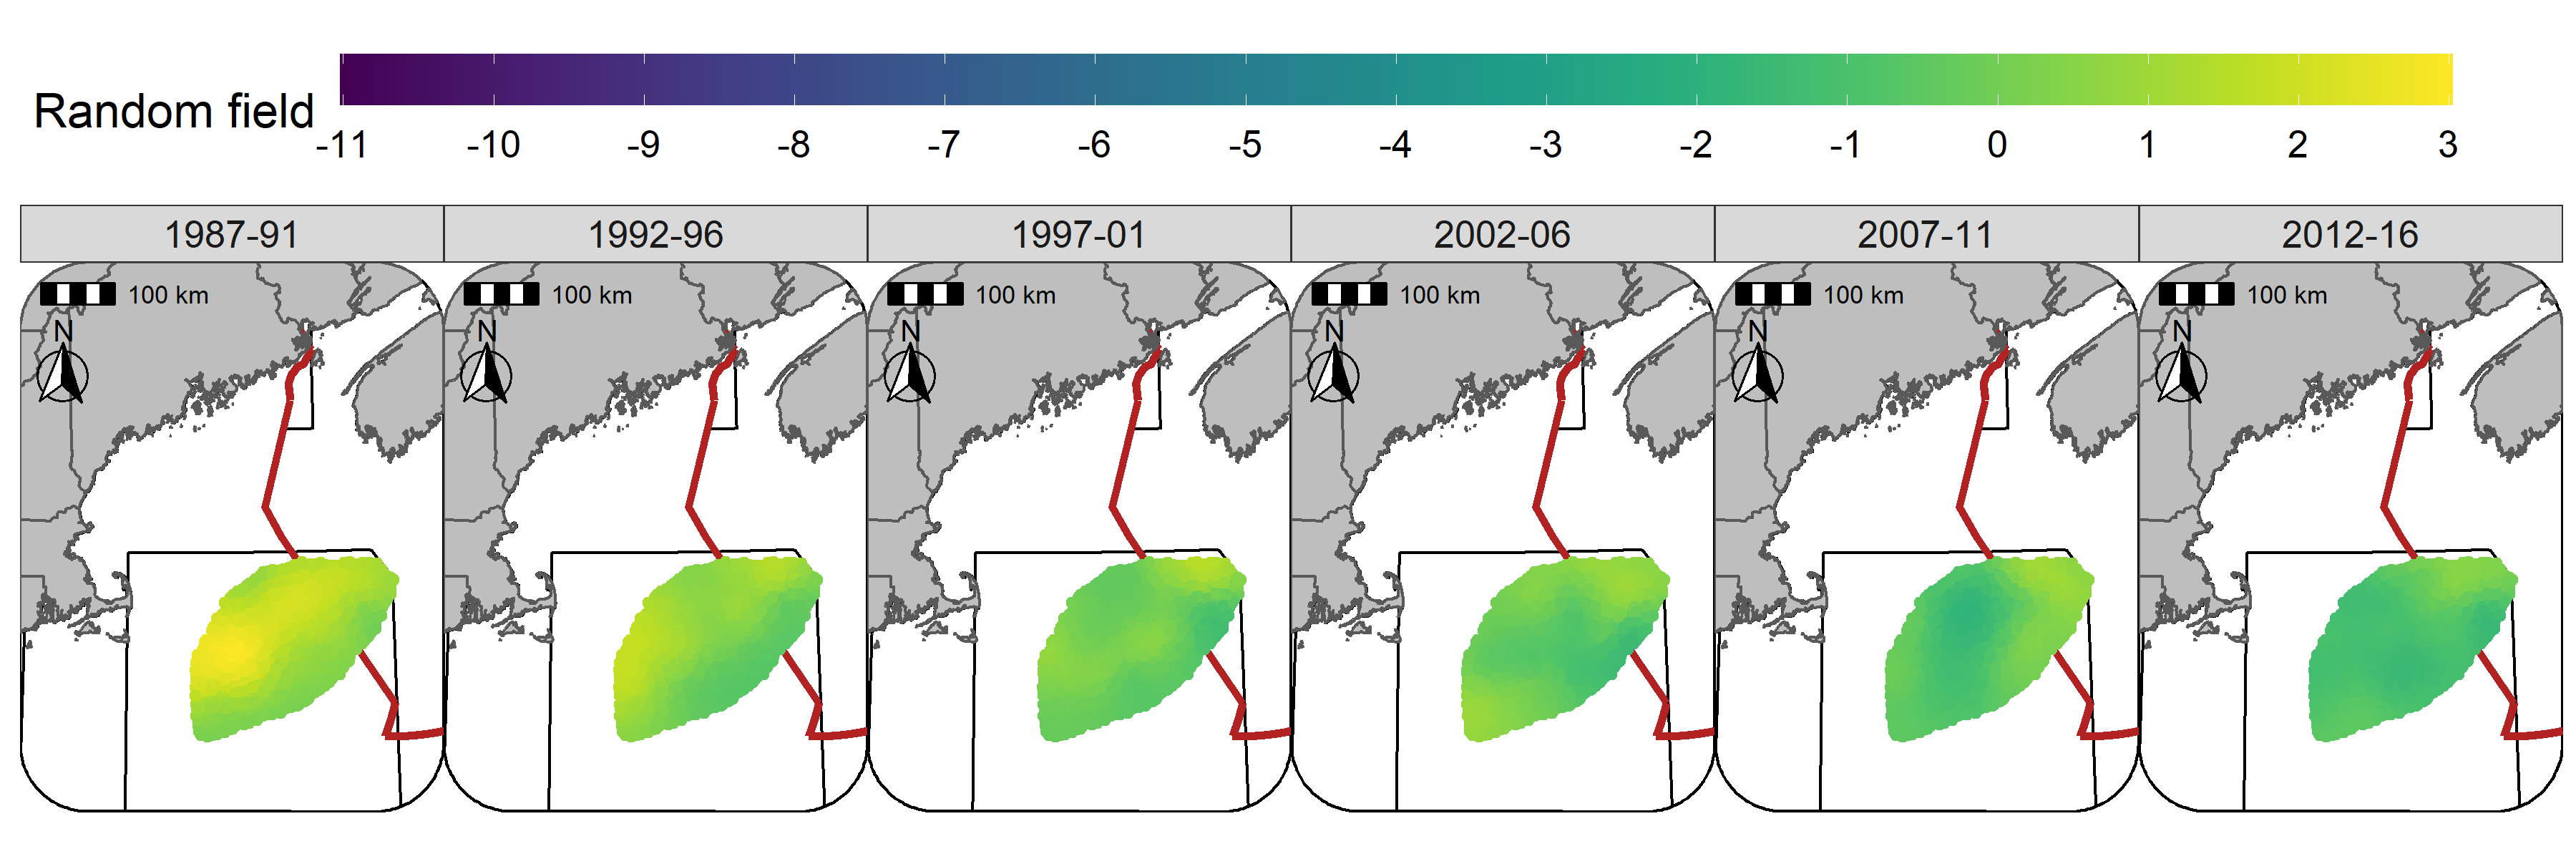
\includegraphics[width=1\linewidth]{D:/Github/Paper_2_SDMs/Results/Figures/rf_winter_cod} 

}

\caption{Random fields (logit scale) for Atlantic Cod  in each era during the Winter (RV survey) using the SST + Depth model and 5 year random field.}\label{fig:rf-winter-cod}
\end{figure}

\newpage
\begin{figure}[htb]

{\centering 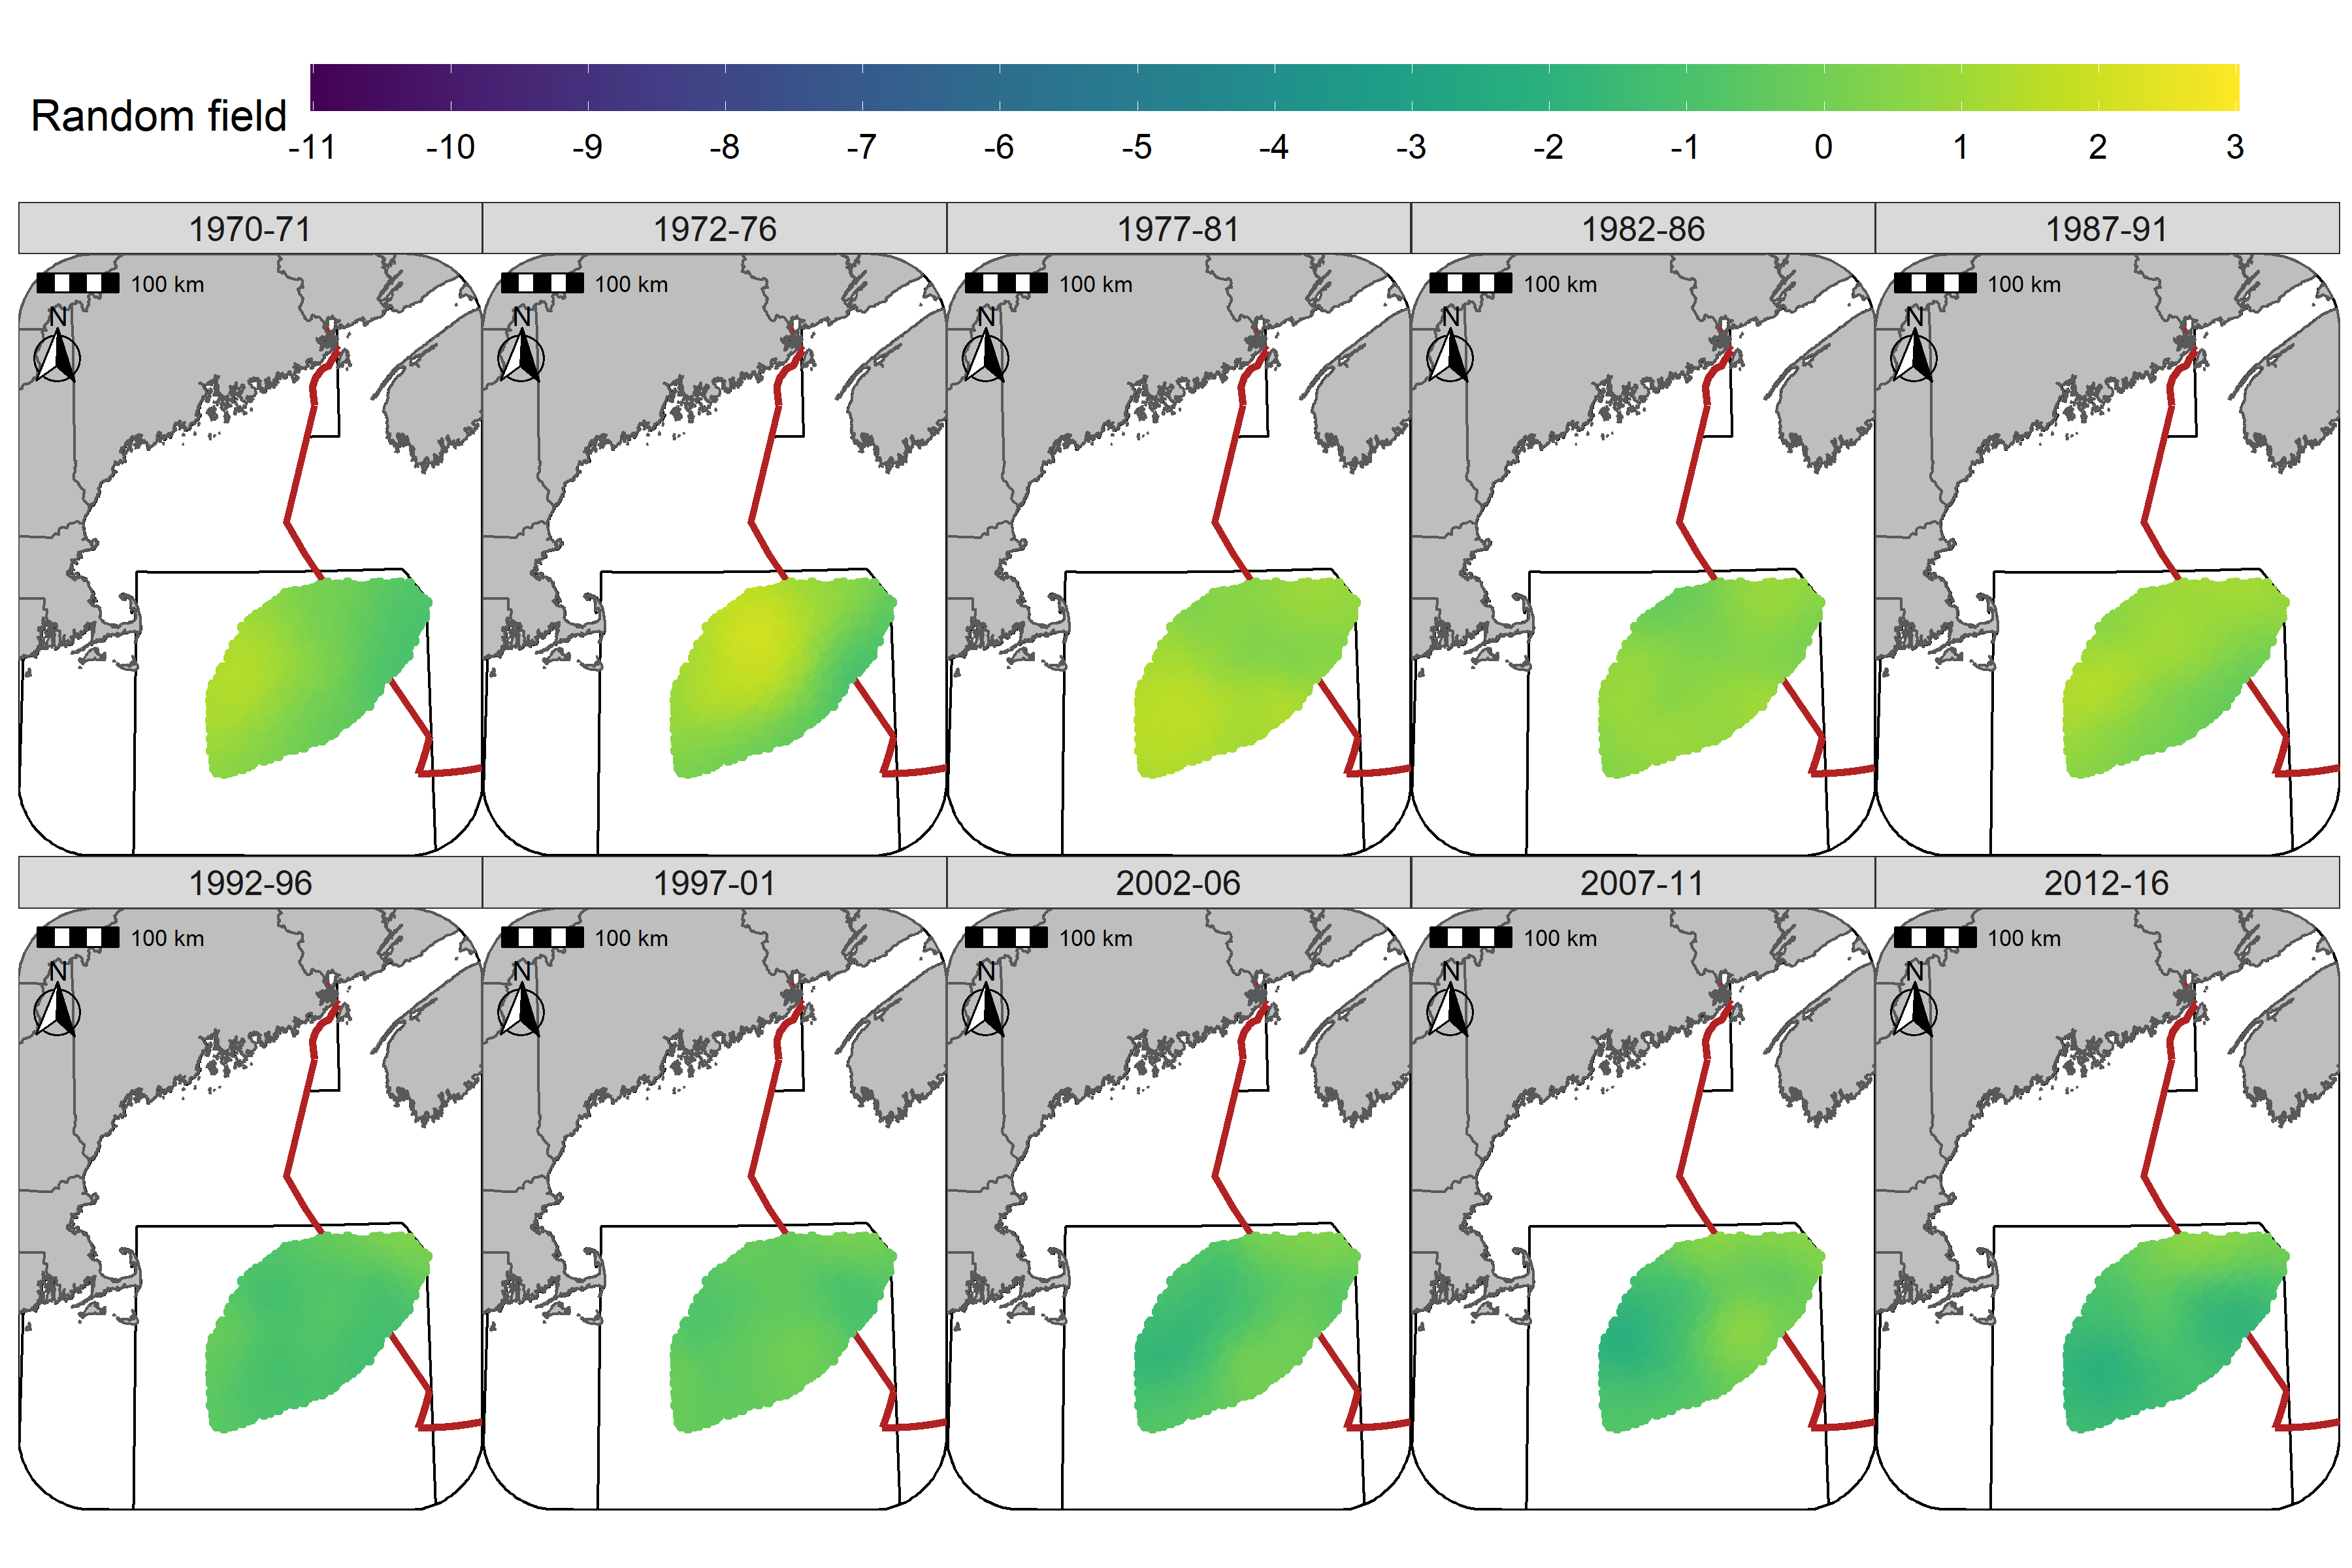
\includegraphics[width=1\linewidth]{D:/Github/Paper_2_SDMs/Results/Figures/rf_spring_cod} 

}

\caption{Random fields (logit scale) for Atlantic Cod  in each era during the Spring (NMFS-spring survey) using the SST + Depth model and 5 year random field.}\label{fig:rf-spring-cod}
\end{figure}

\newpage
\begin{figure}[htb]

{\centering 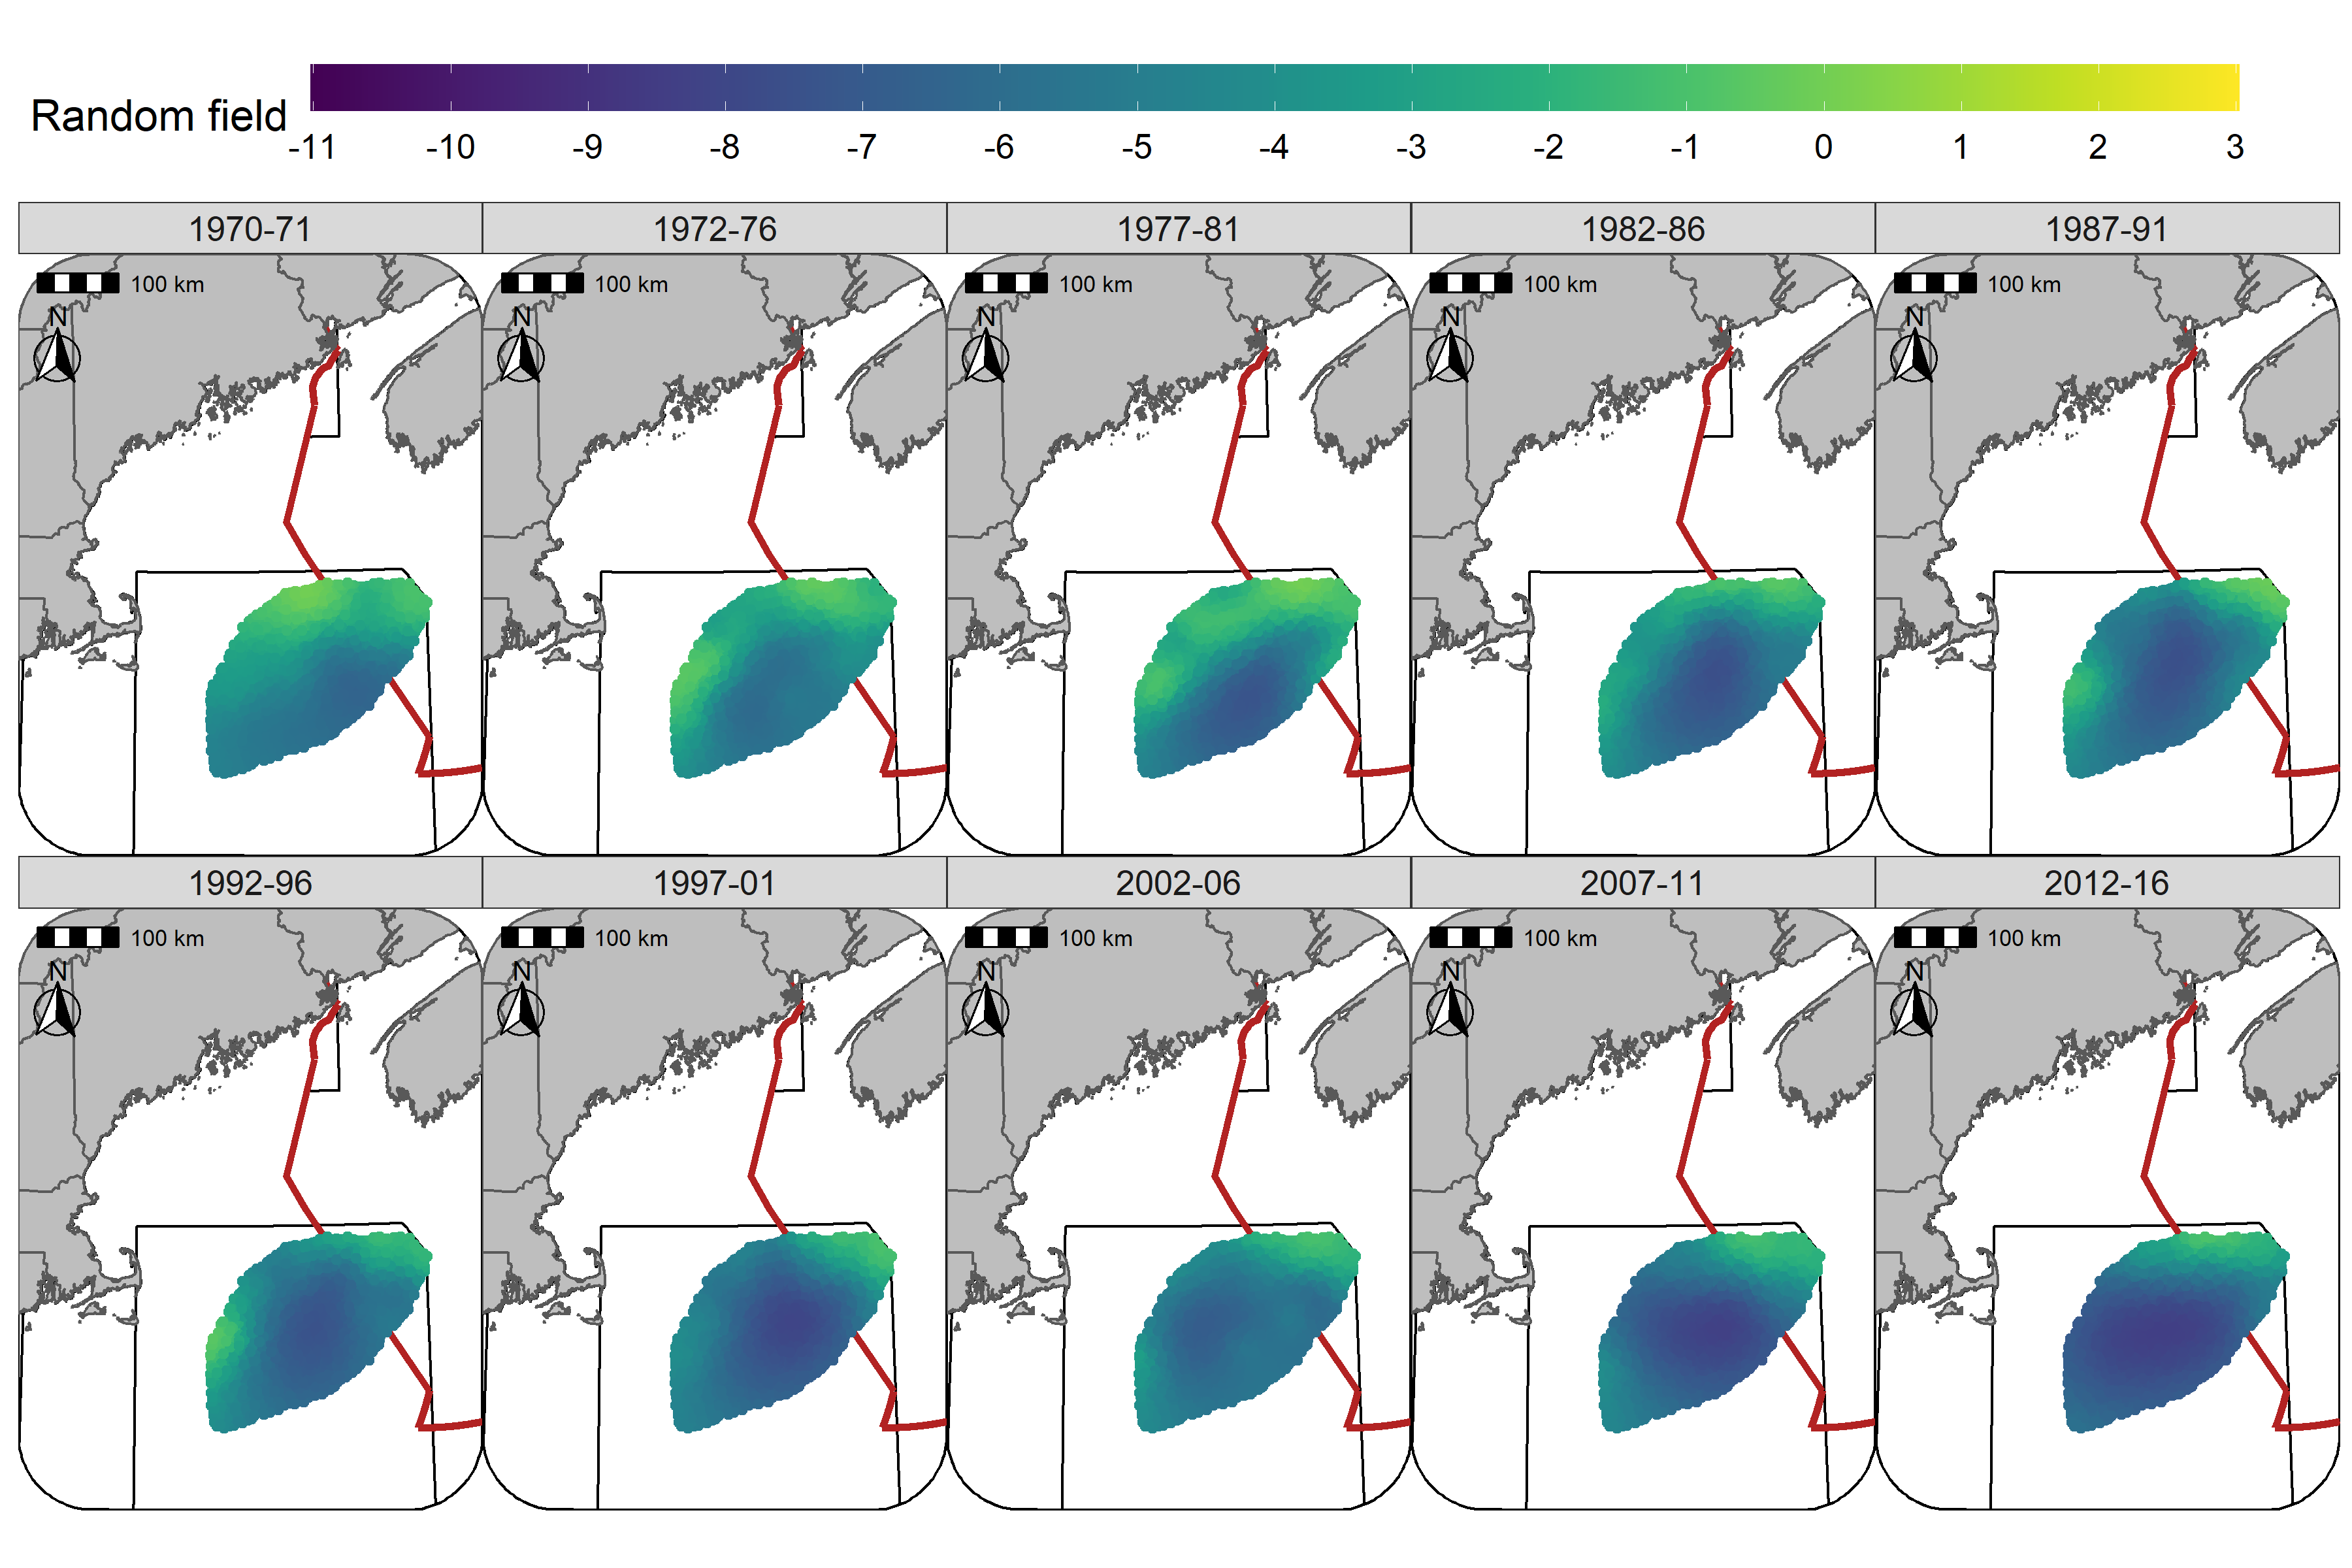
\includegraphics[width=1\linewidth]{D:/Github/Paper_2_SDMs/Results/Figures/rf_fall_cod} 

}

\caption{Random fields (logit scale) for Atlantic Cod  in each era during the Fall (NMFS-fall survey) using the SST + Depth model and 5 year random field.}\label{fig:rf-fall-cod}
\end{figure}

\newpage
\begin{figure}[htb]

{\centering 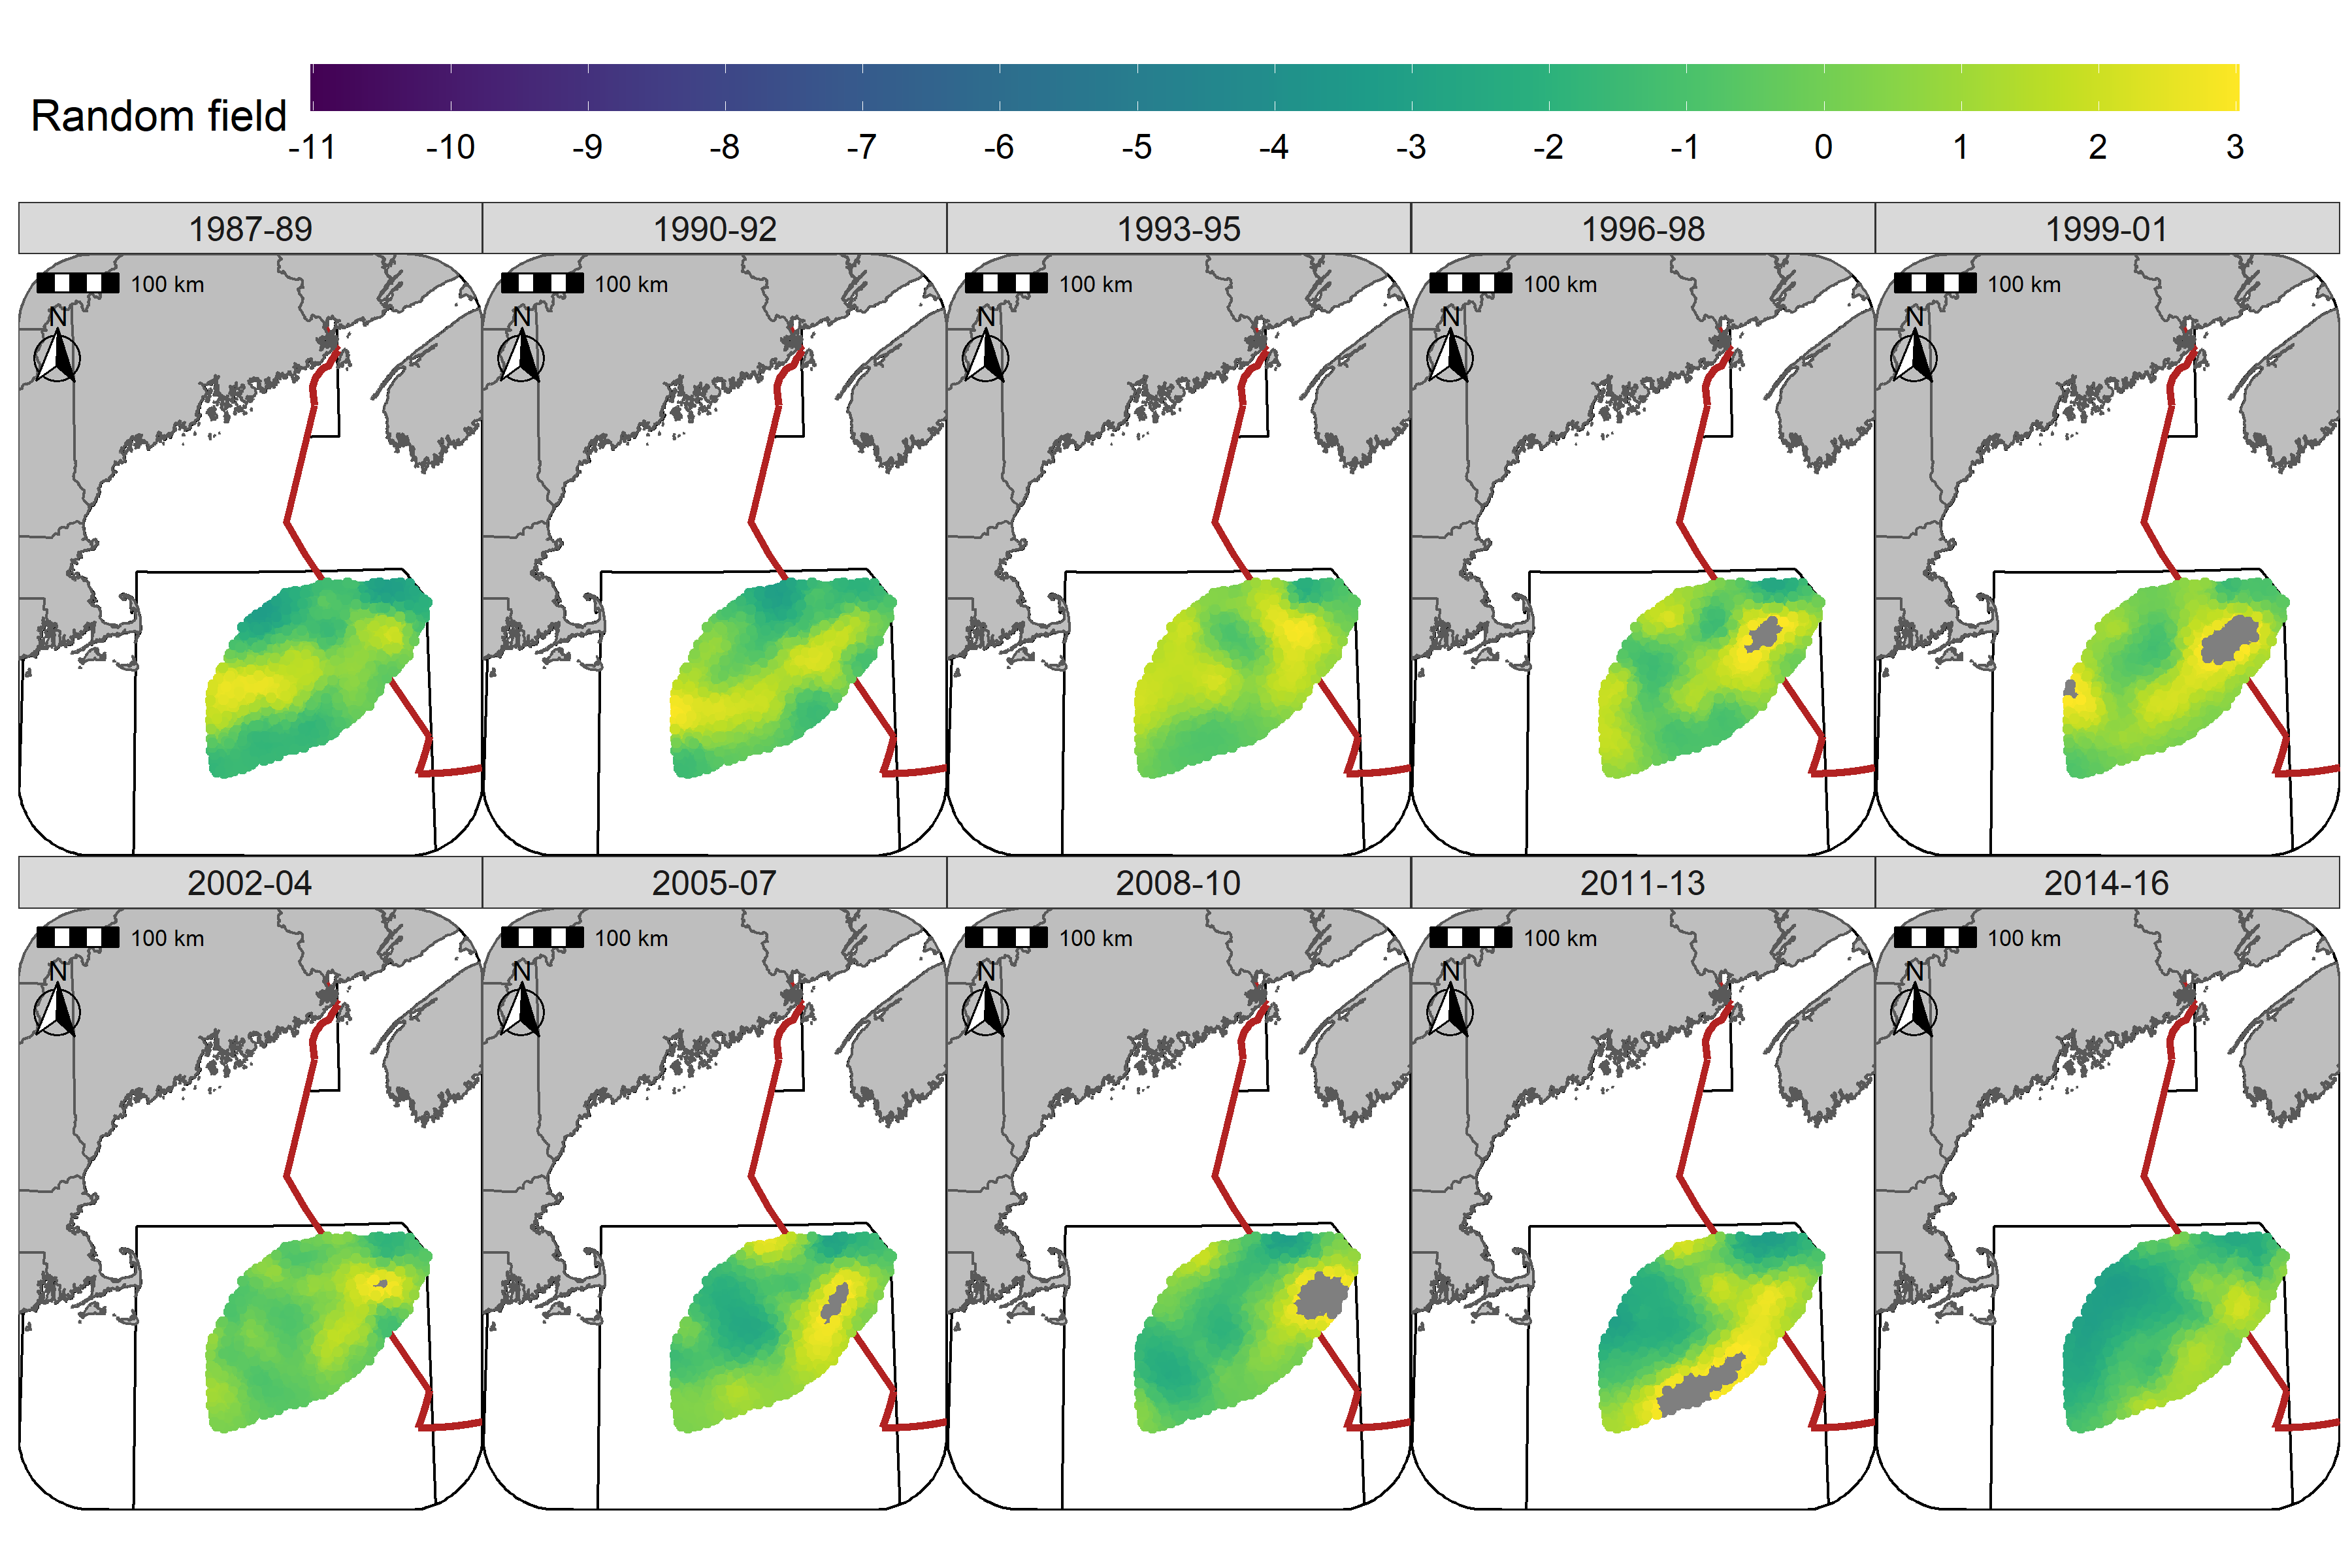
\includegraphics[width=1\linewidth]{D:/Github/Paper_2_SDMs/Results/Figures/rf_winter_yt} 

}

\caption{Random fields (logit scale) for Yellowtail Flounder in each era during the Winter (RV survey) using the SST + Depth + Sed model and 3 year random field.}\label{fig:rf-winter-yt}
\end{figure}

\newpage
\begin{figure}[htb]

{\centering 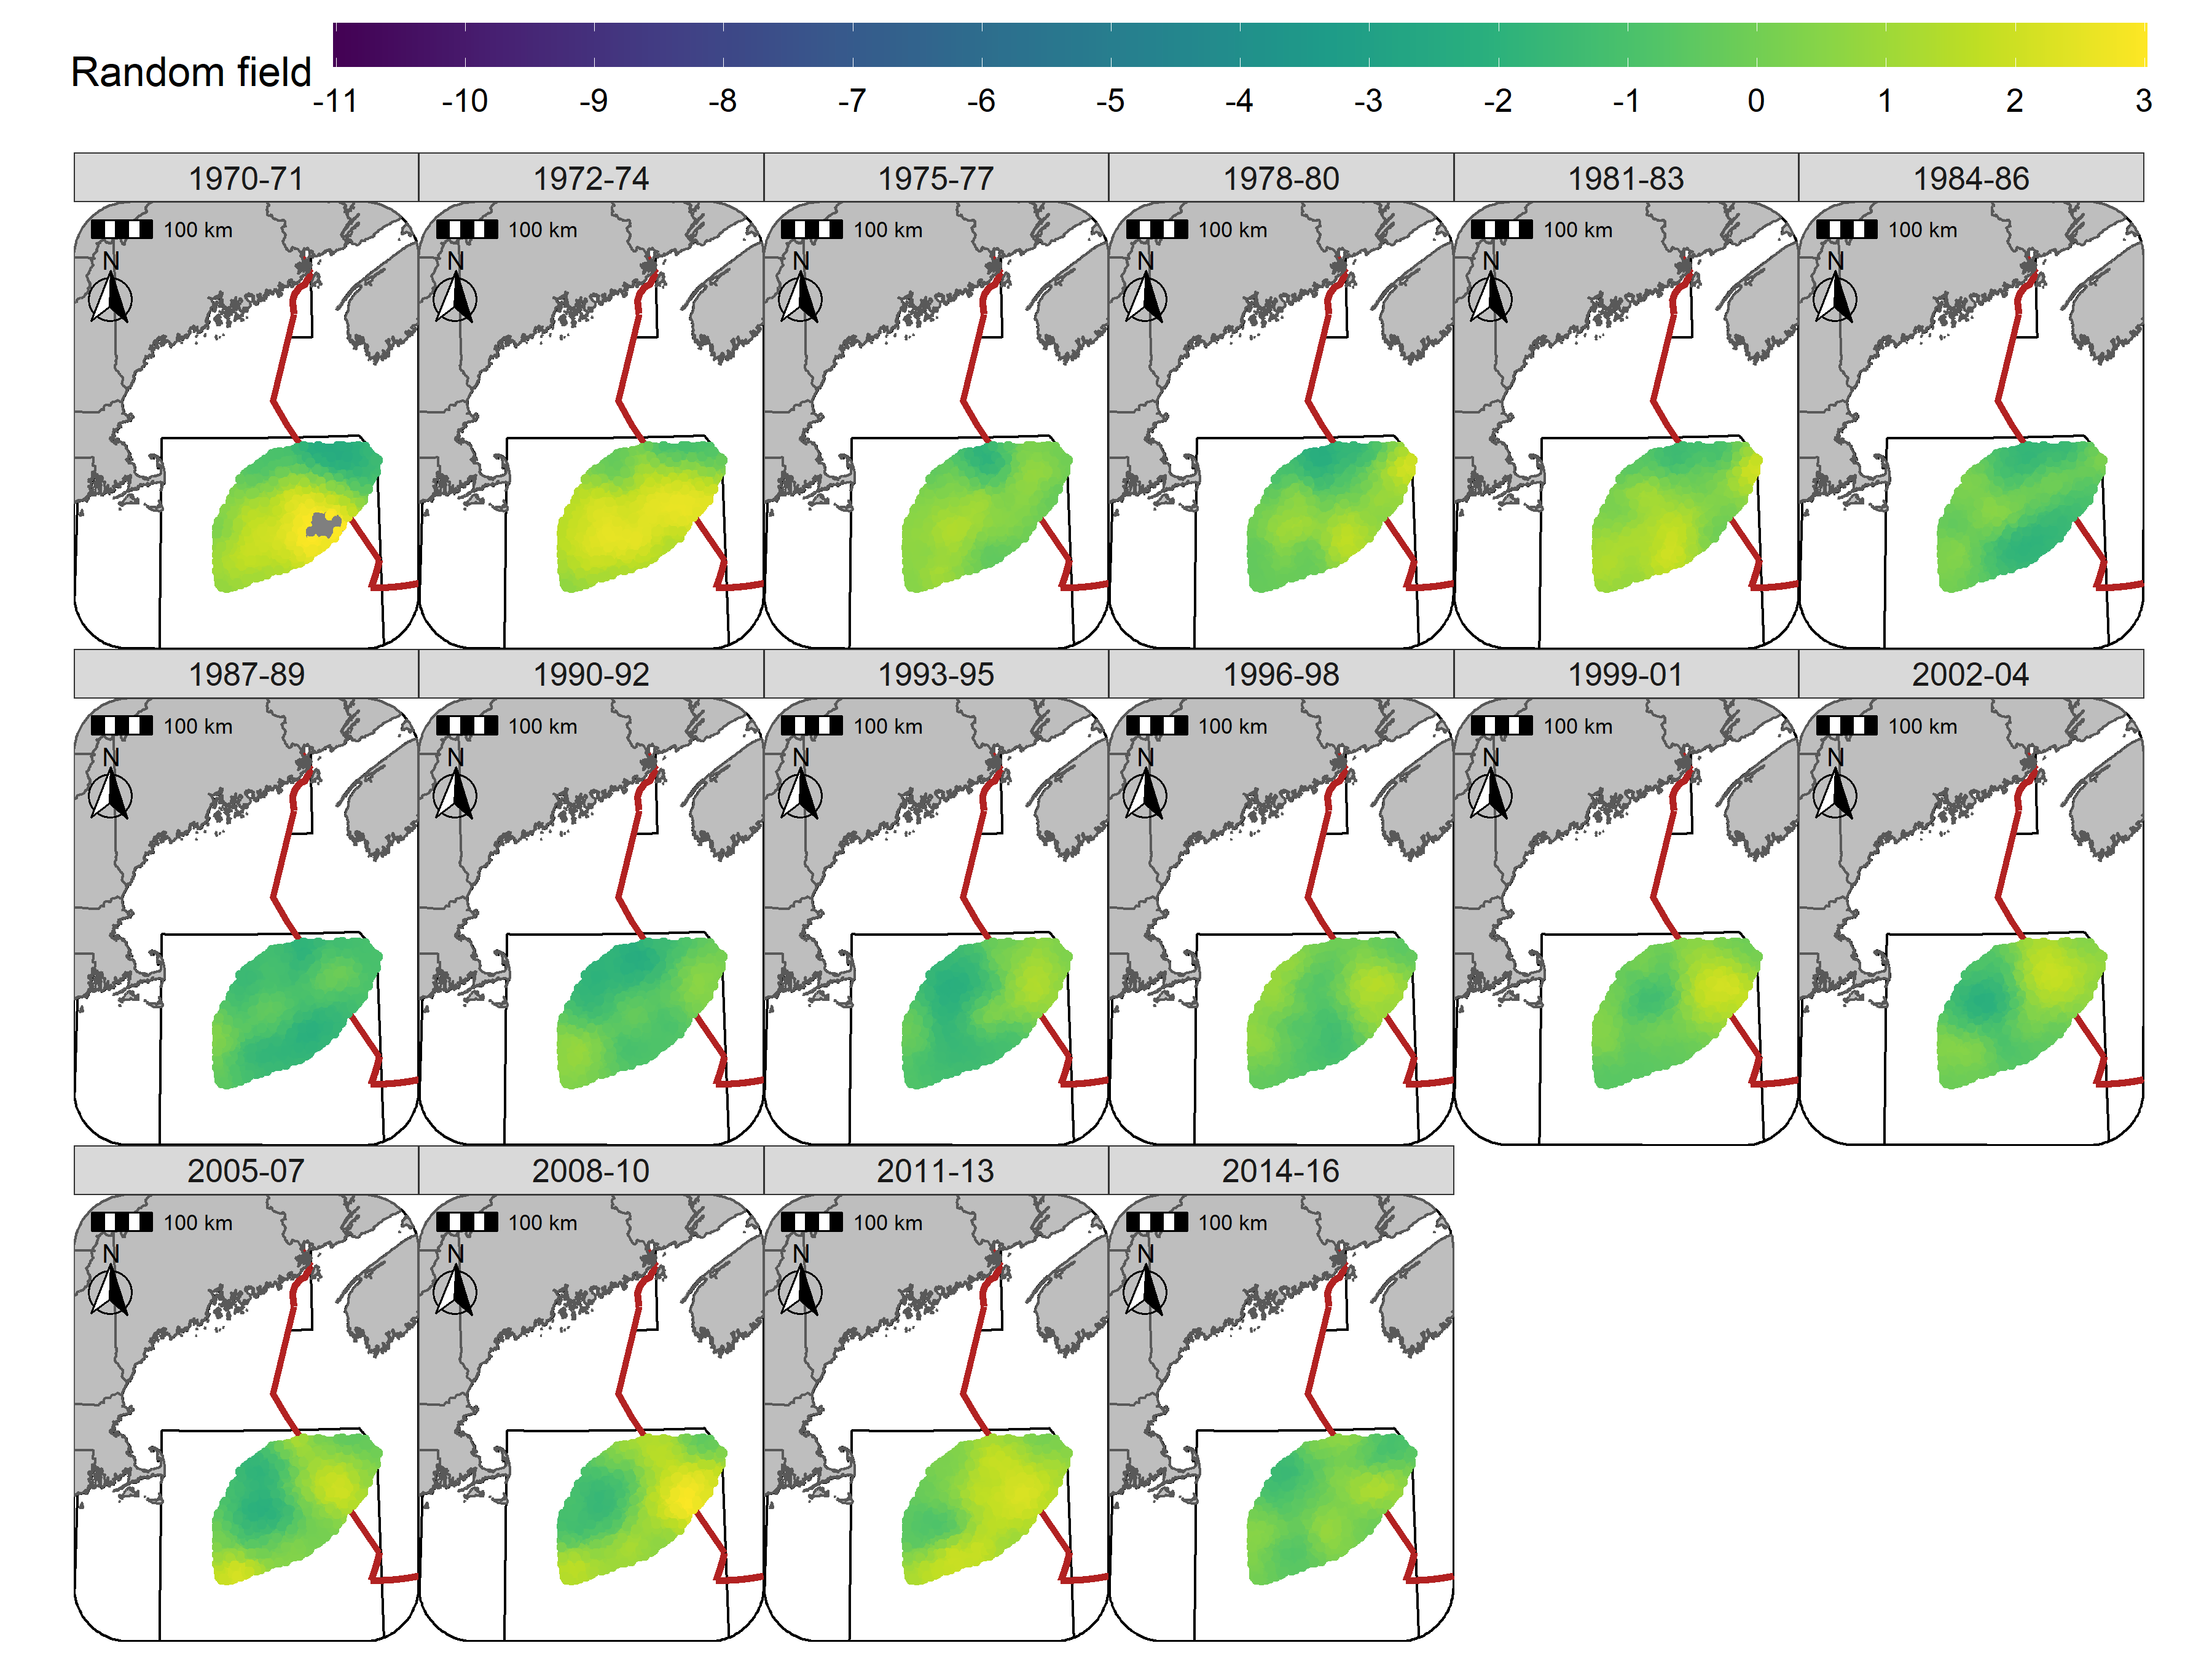
\includegraphics[width=1\linewidth]{D:/Github/Paper_2_SDMs/Results/Figures/rf_spring_yt} 

}

\caption{Random fields (logit scale) for Yellowtail Flounder in each era during the Spring (NMFS-spring survey) using the SST + Depth + Sed model and 3 year random field.}\label{fig:rf-spring-yt}
\end{figure}

\newpage
\begin{figure}[htb]

{\centering 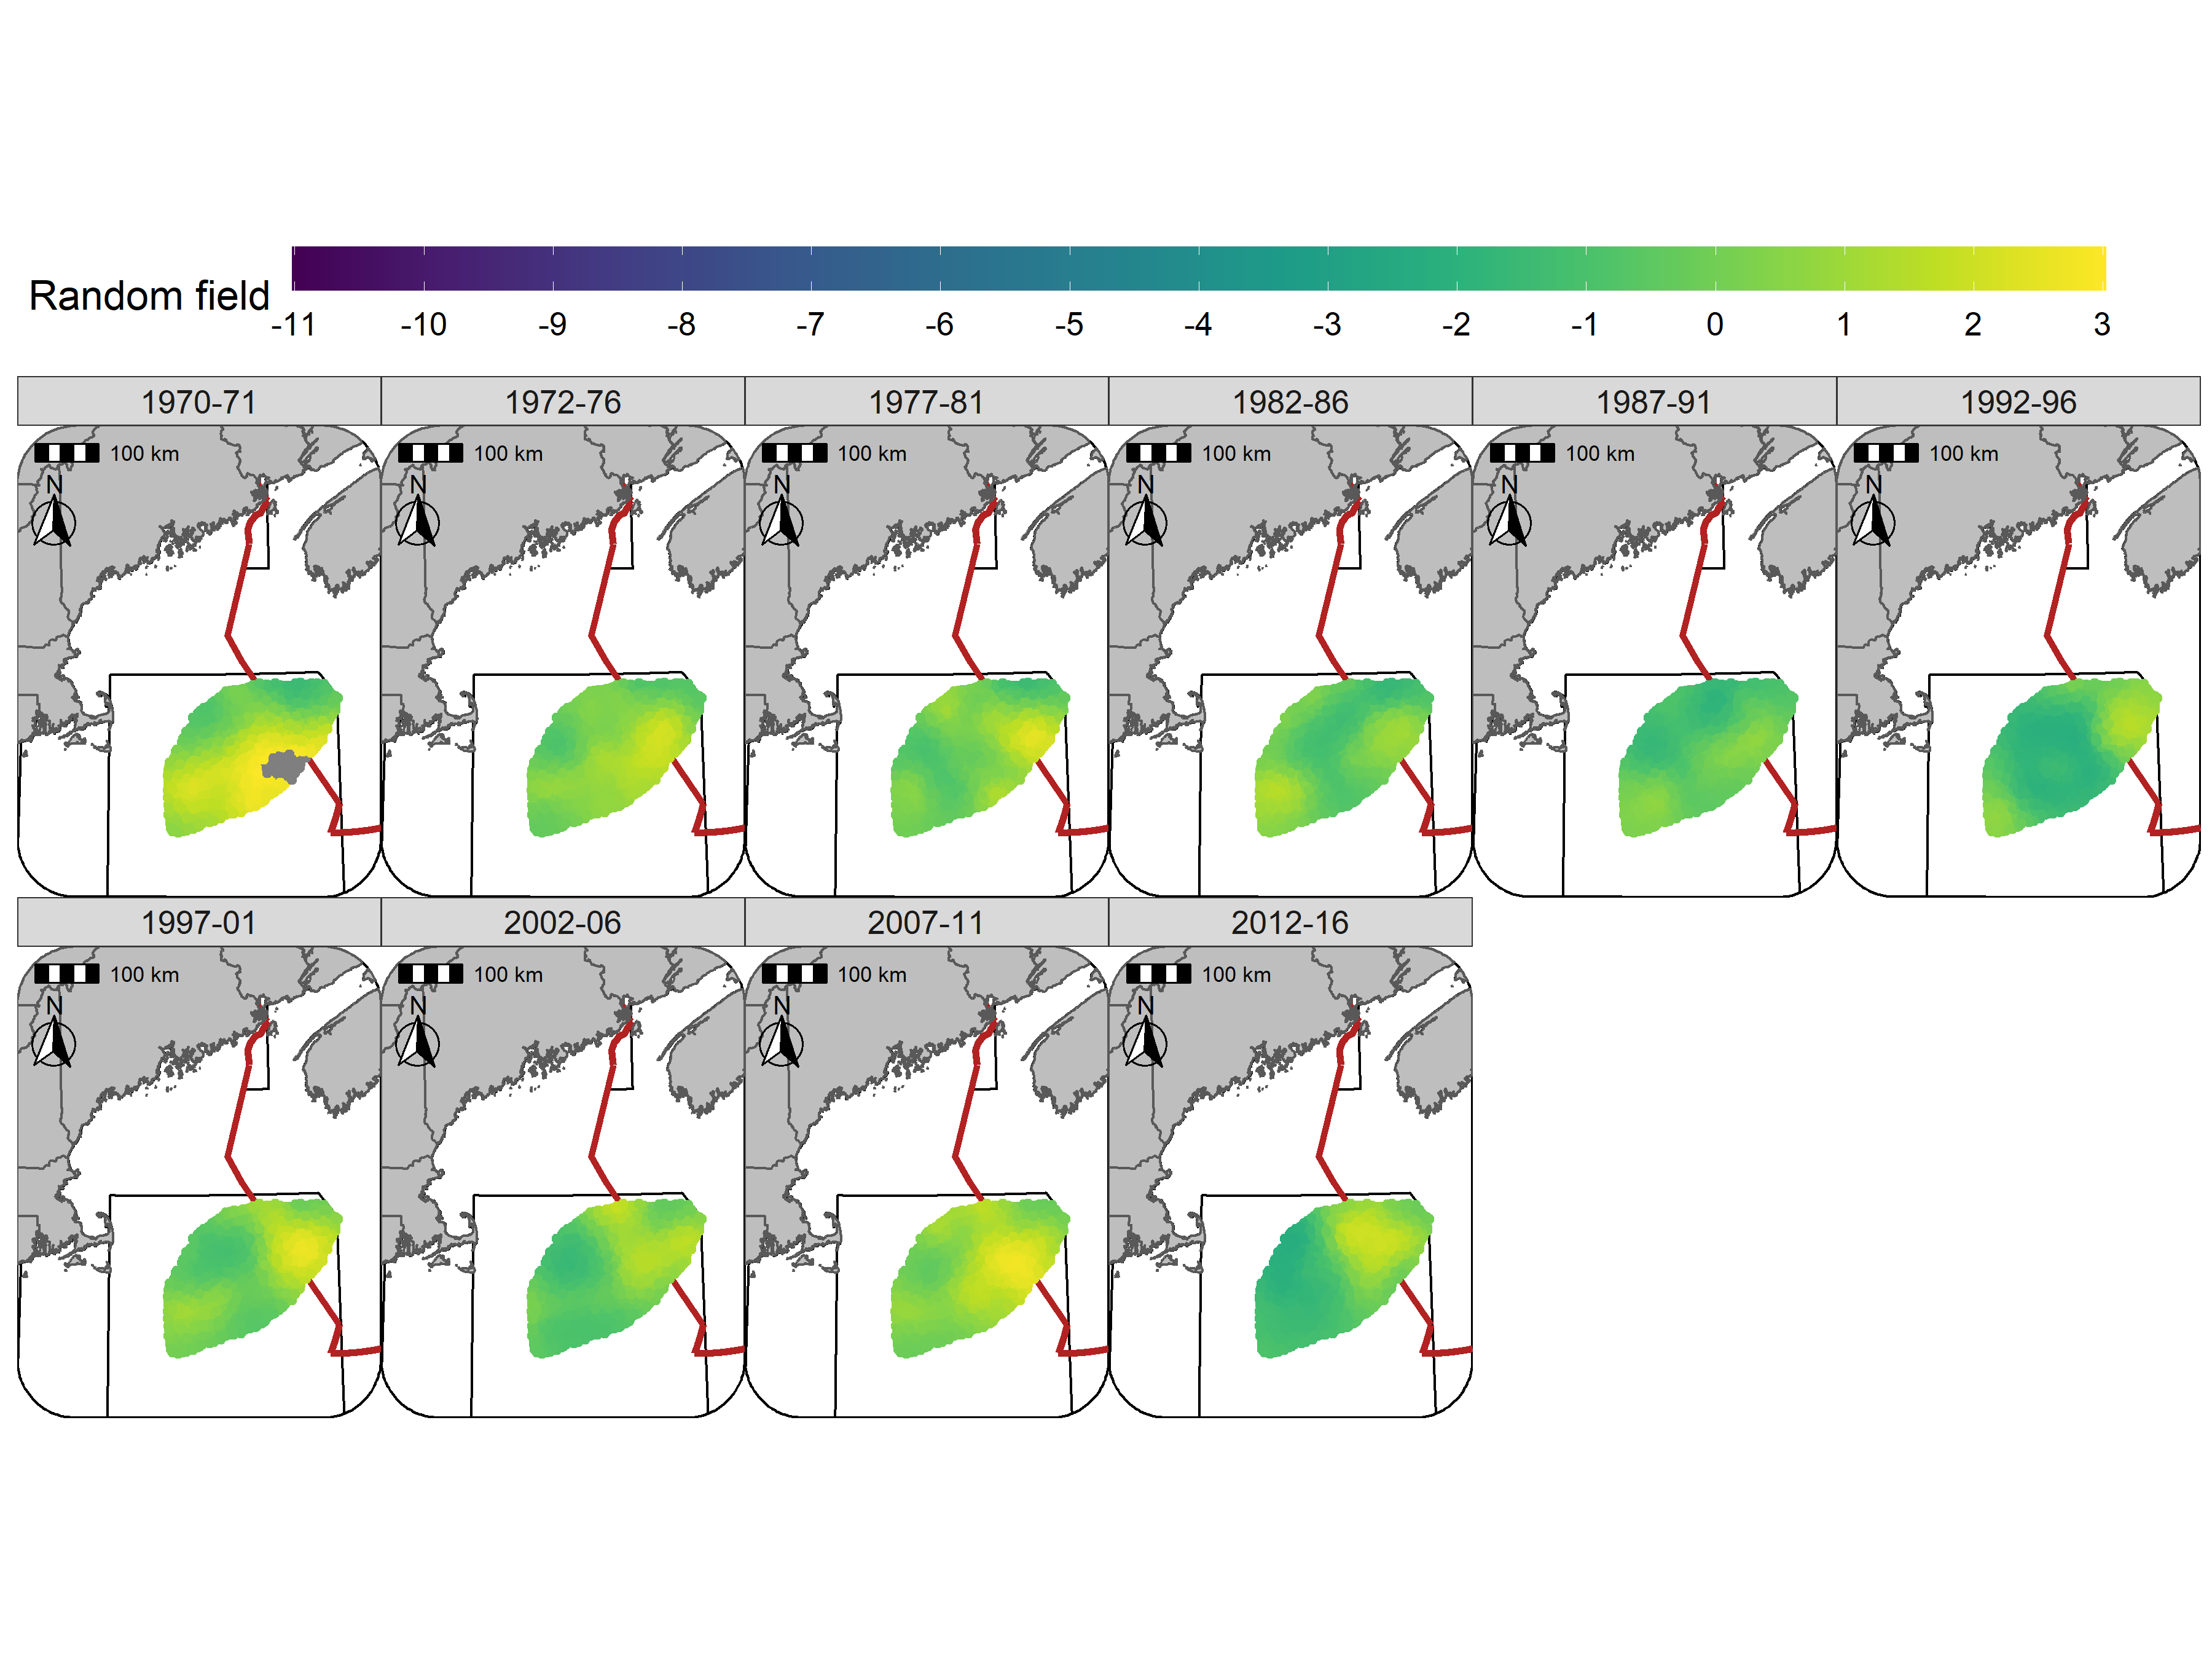
\includegraphics[width=1\linewidth]{D:/Github/Paper_2_SDMs/Results/Figures/rf_fall_yt} 

}

\caption{Random fields (logit scale) for Yellowtail Flounder in each era during the Fall (NMFS-fall survey) using the SST + Depth + Sed model and 5 year random field.}\label{fig:rf-fall-yt}
\end{figure}

\newpage

\begin{figure}[htb]

{\centering 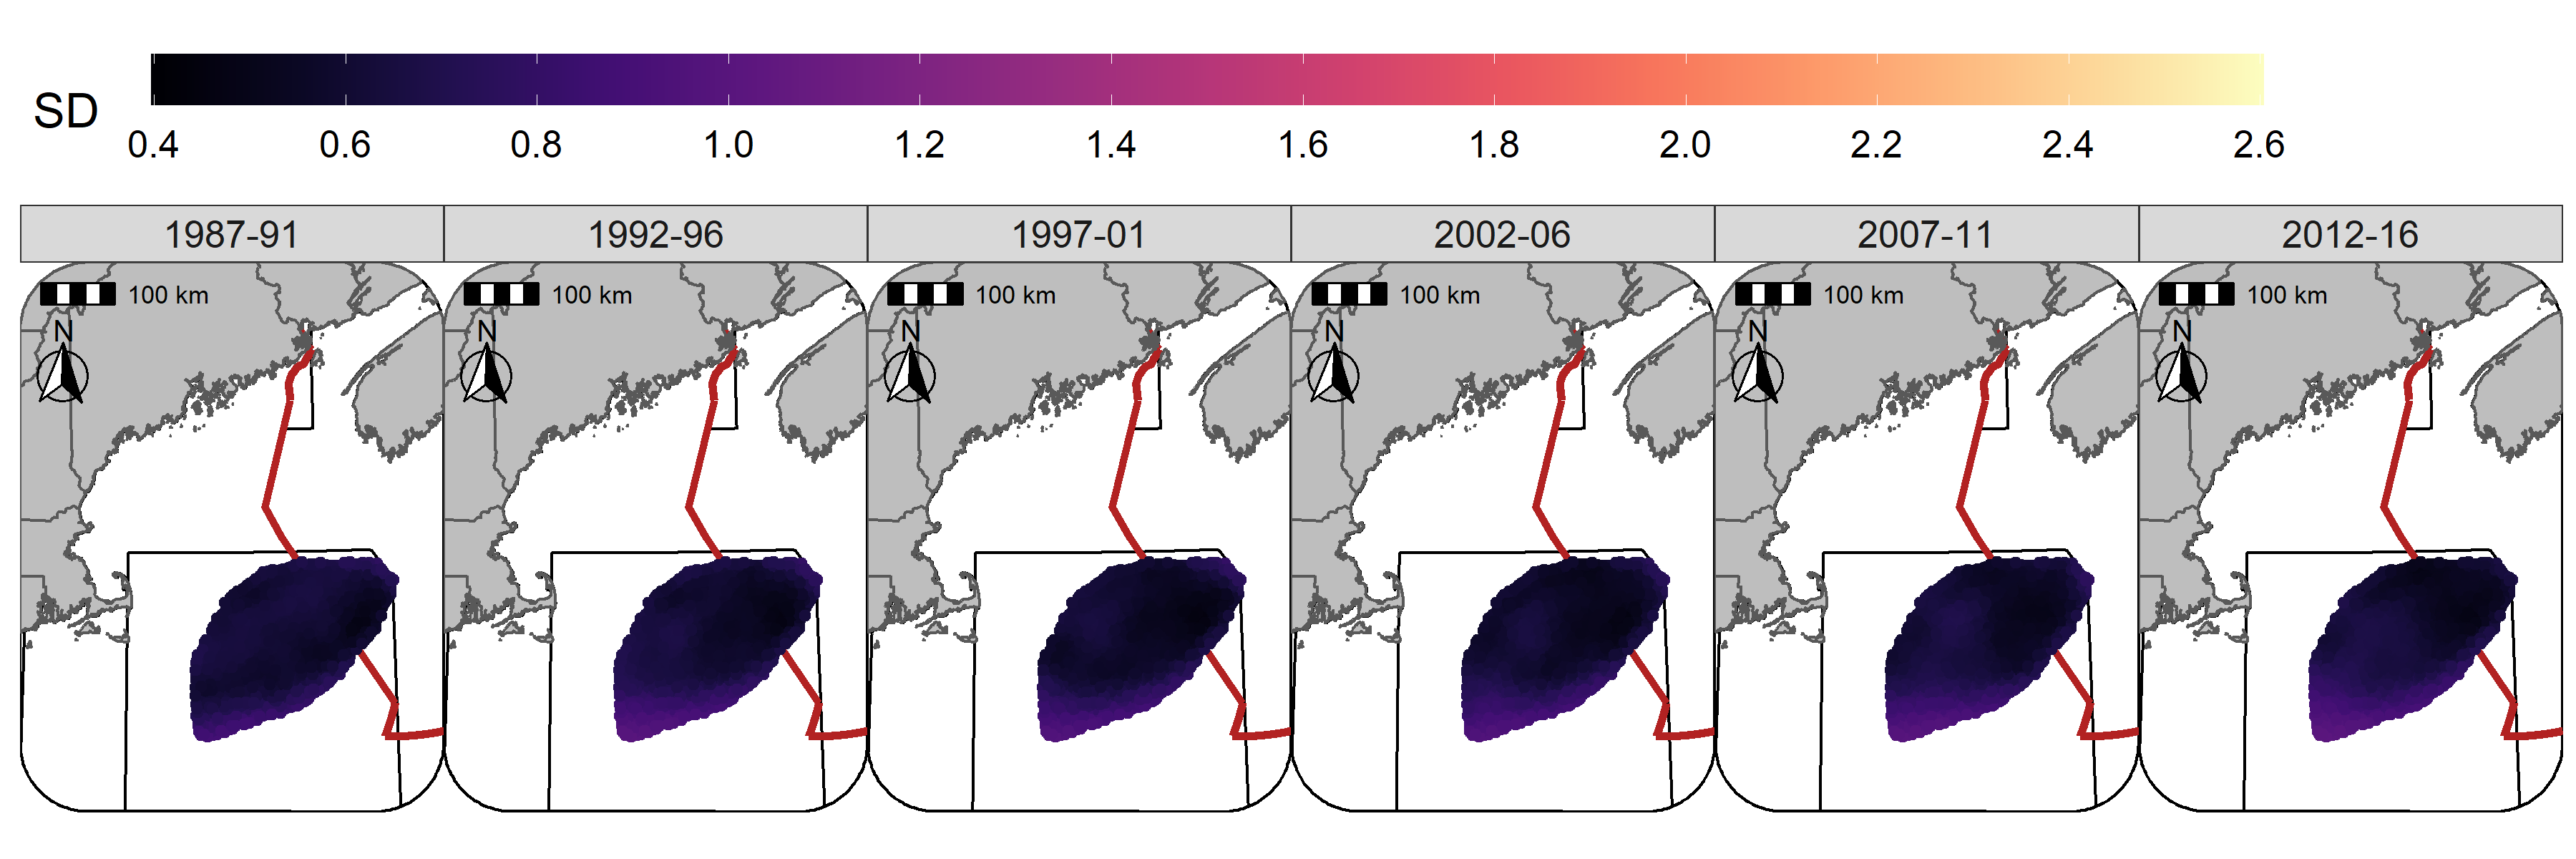
\includegraphics[width=1\linewidth]{D:/Github/Paper_2_SDMs/Results/Figures/rf_winter_cod_sd} 

}

\caption{Standard deviation of random fields (logit scale) for Atlantic Cod  in each era during the Winter (RV survey) using the SST + Depth model and 5 year random field.}\label{fig:rf-winter-cod-sd}
\end{figure}

\newpage
\begin{figure}[htb]

{\centering 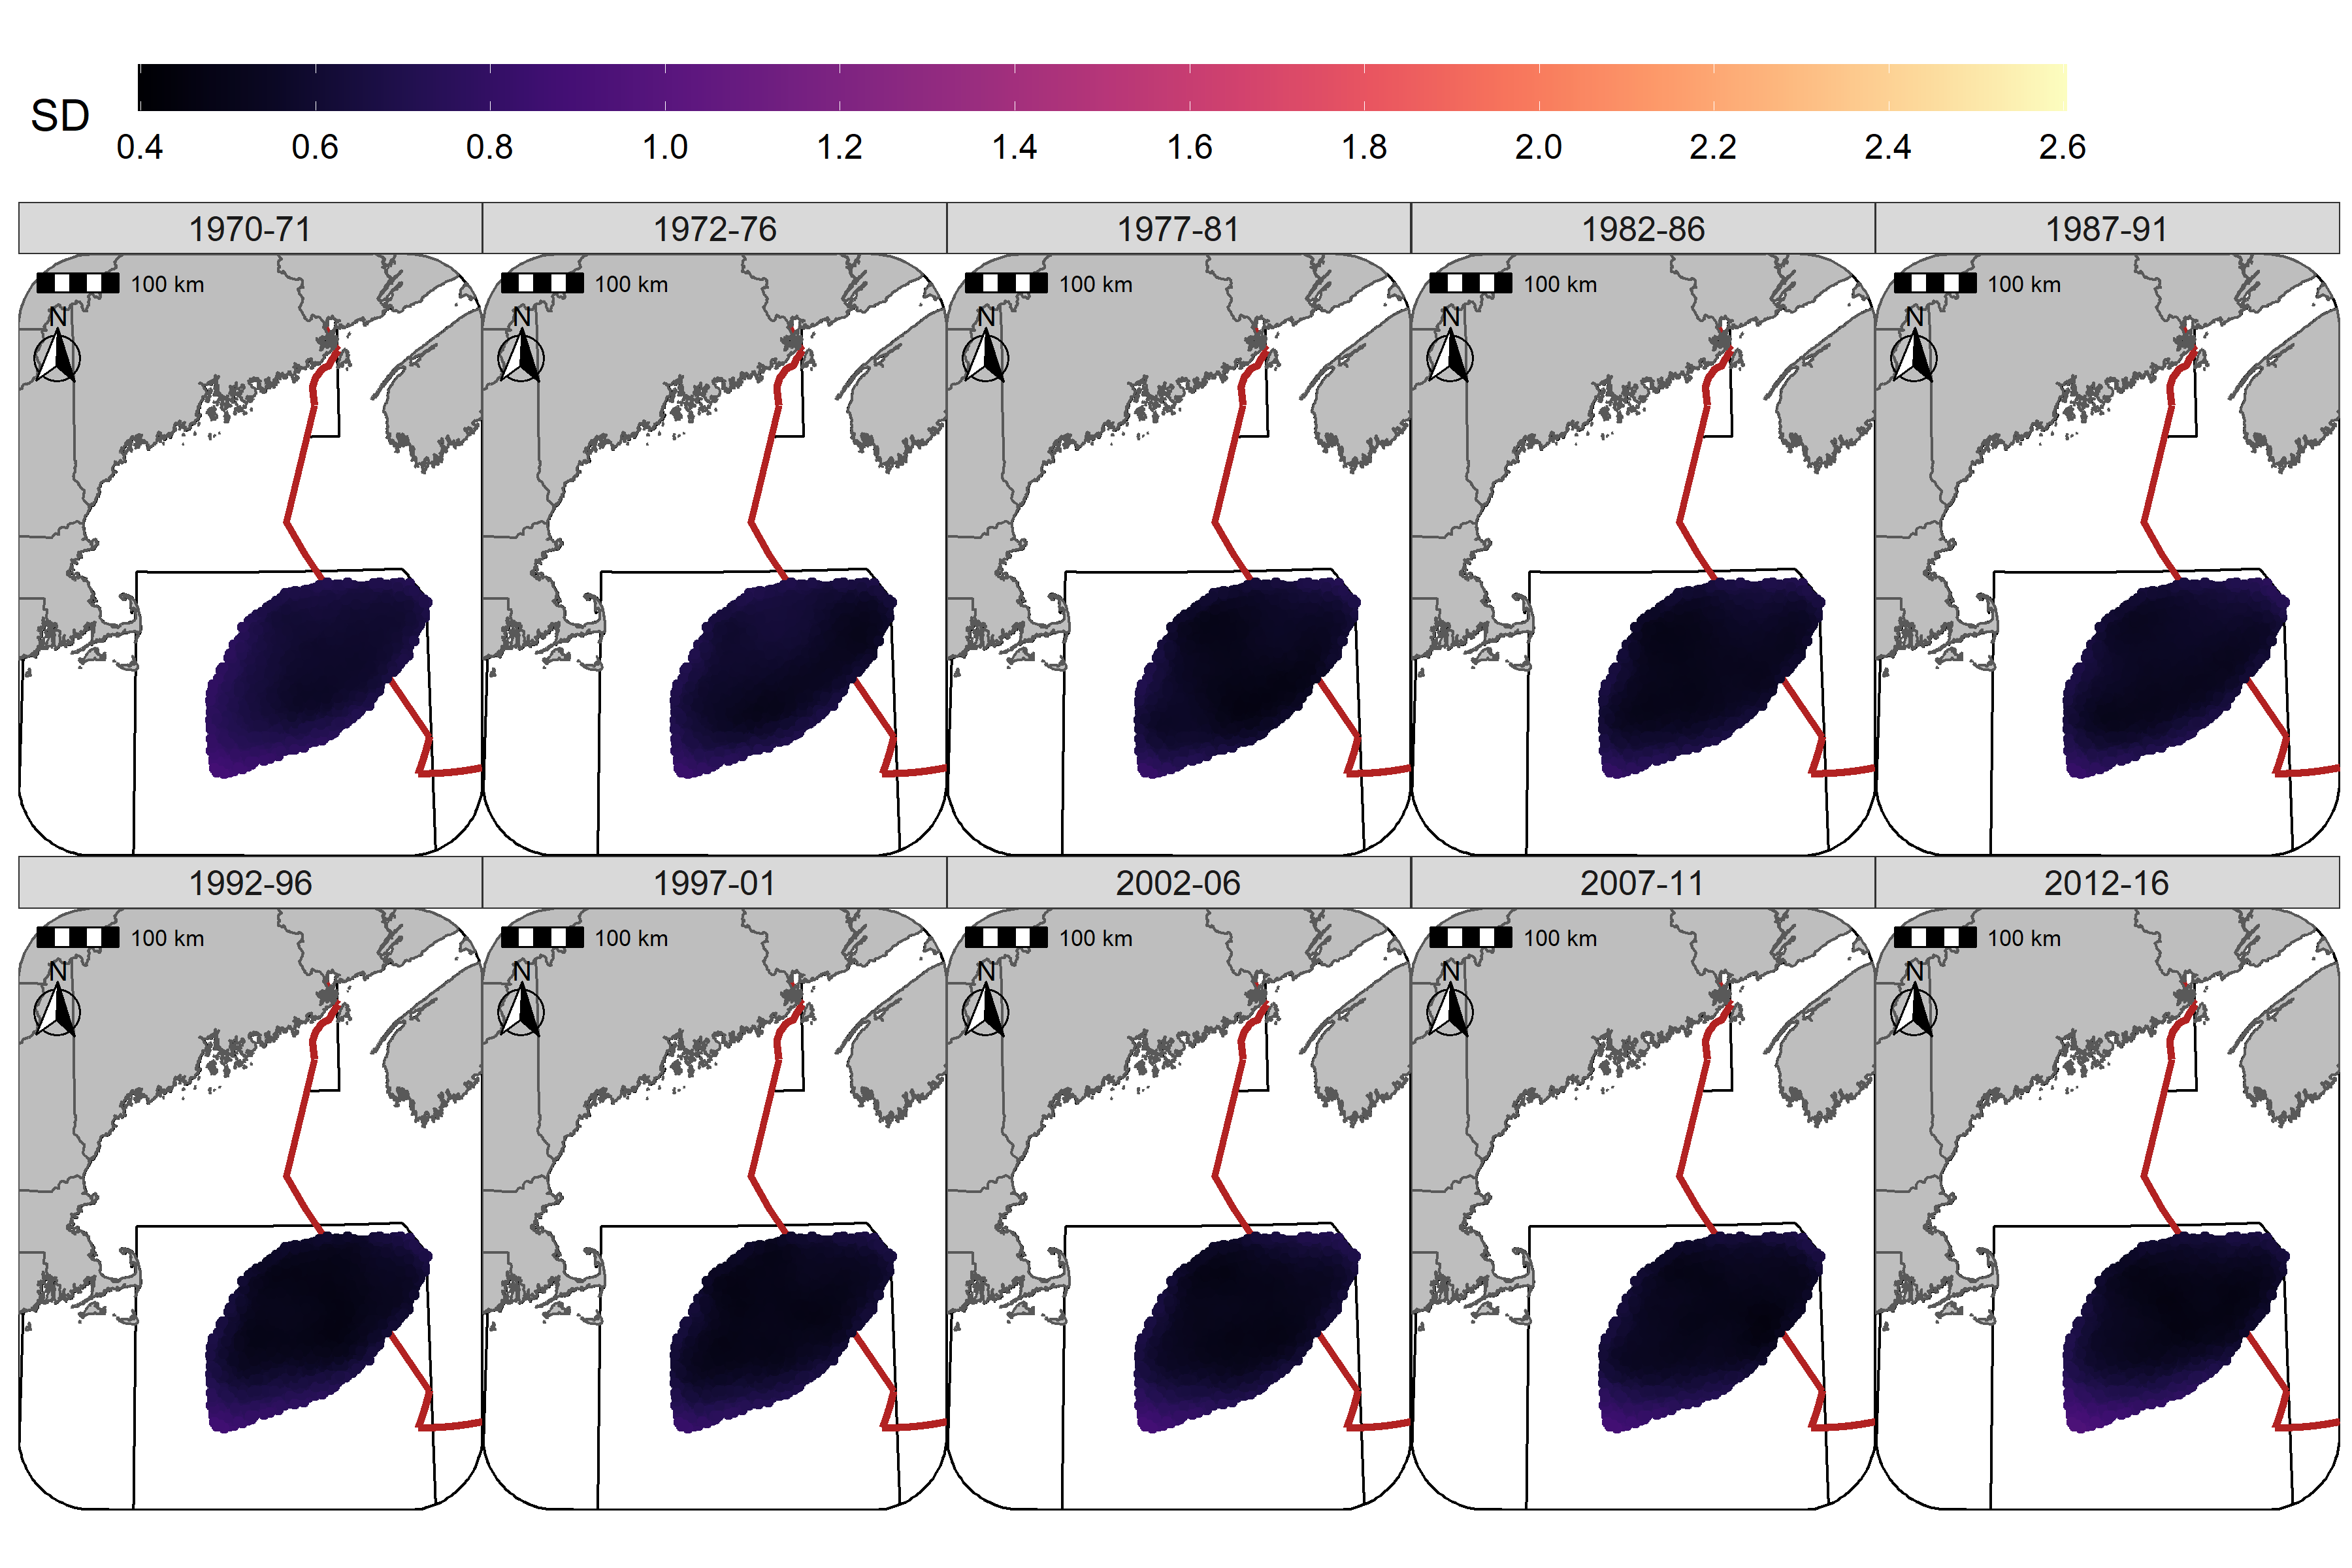
\includegraphics[width=1\linewidth]{D:/Github/Paper_2_SDMs/Results/Figures/rf_spring_cod_sd} 

}

\caption{Standard deviation of random fields (logit scale) for Atlantic Cod  in each era during the Spring (NMFS-spring survey) using the SST + Depth model and 5 year random field.}\label{fig:rf-spring-cod-sd}
\end{figure}

\newpage
\begin{figure}[htb]

{\centering 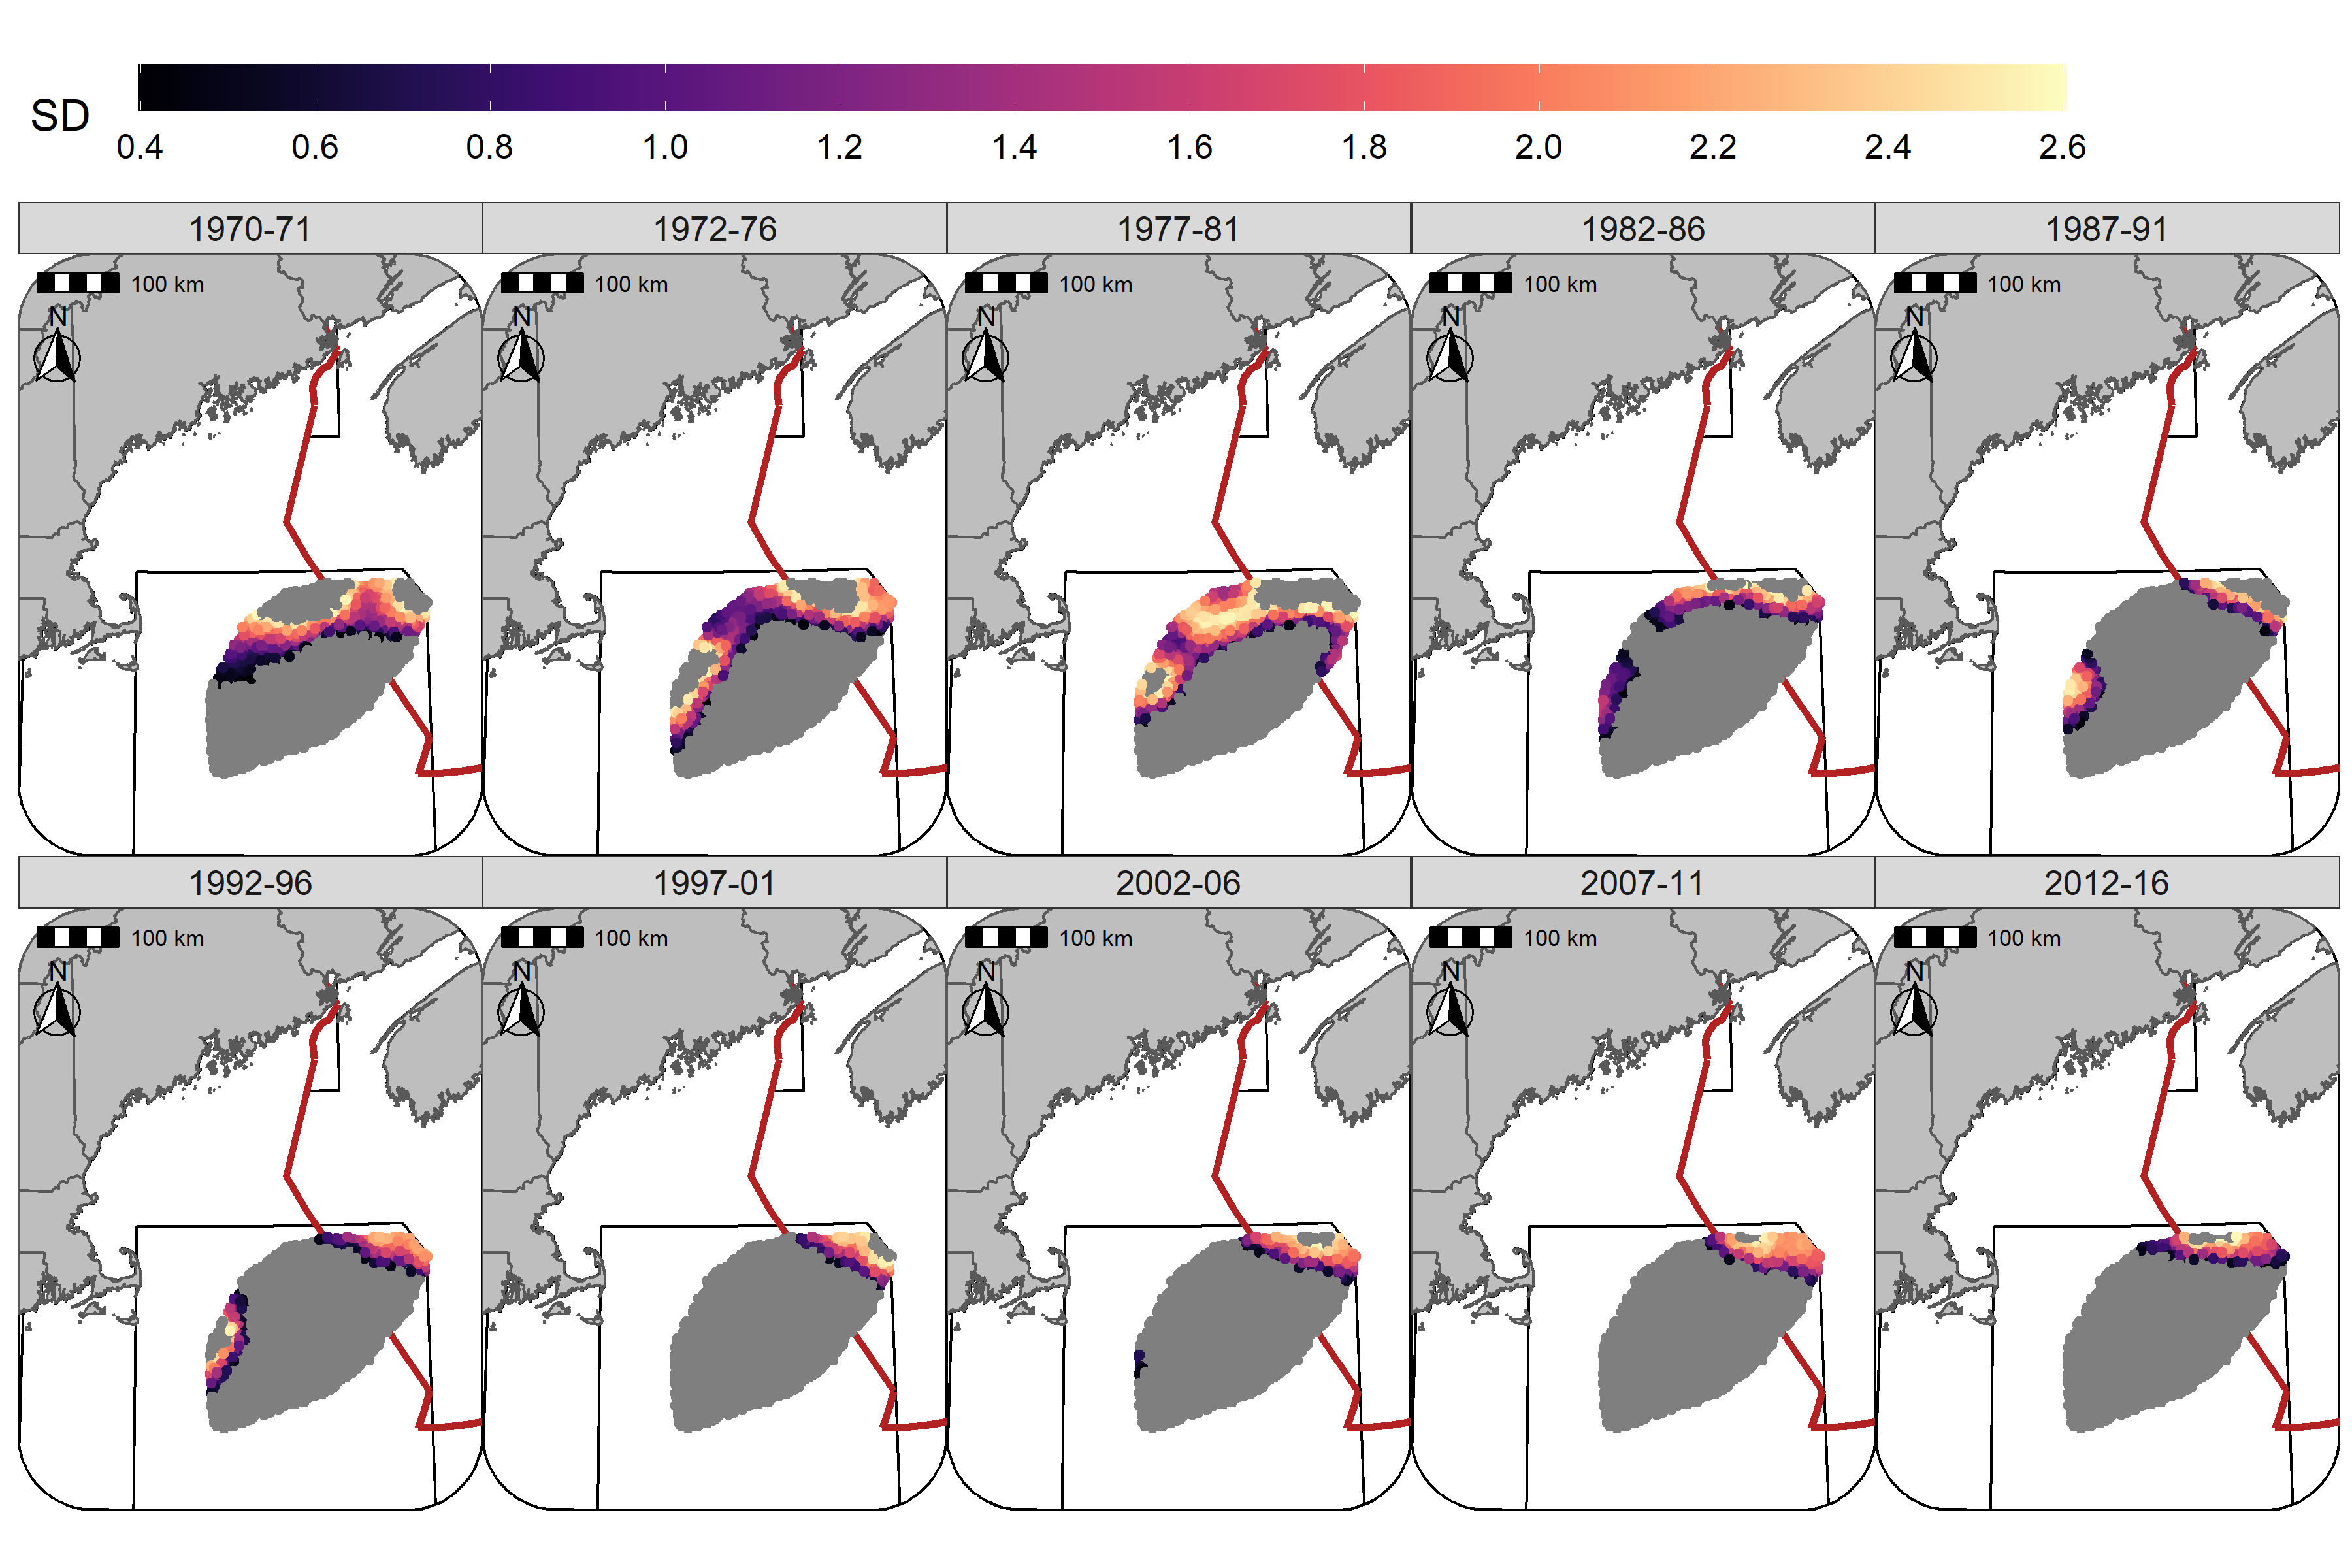
\includegraphics[width=1\linewidth]{D:/Github/Paper_2_SDMs/Results/Figures/rf_fall_cod_sd} 

}

\caption{Standard deviation of random fields (logit scale) for Atlantic Cod  in each era during the Fall (NMFS-fall survey) using the SST + Depth model and 5 year random field.}\label{fig:rf-fall-cod-sd}
\end{figure}

\newpage
\begin{figure}[htb]

{\centering 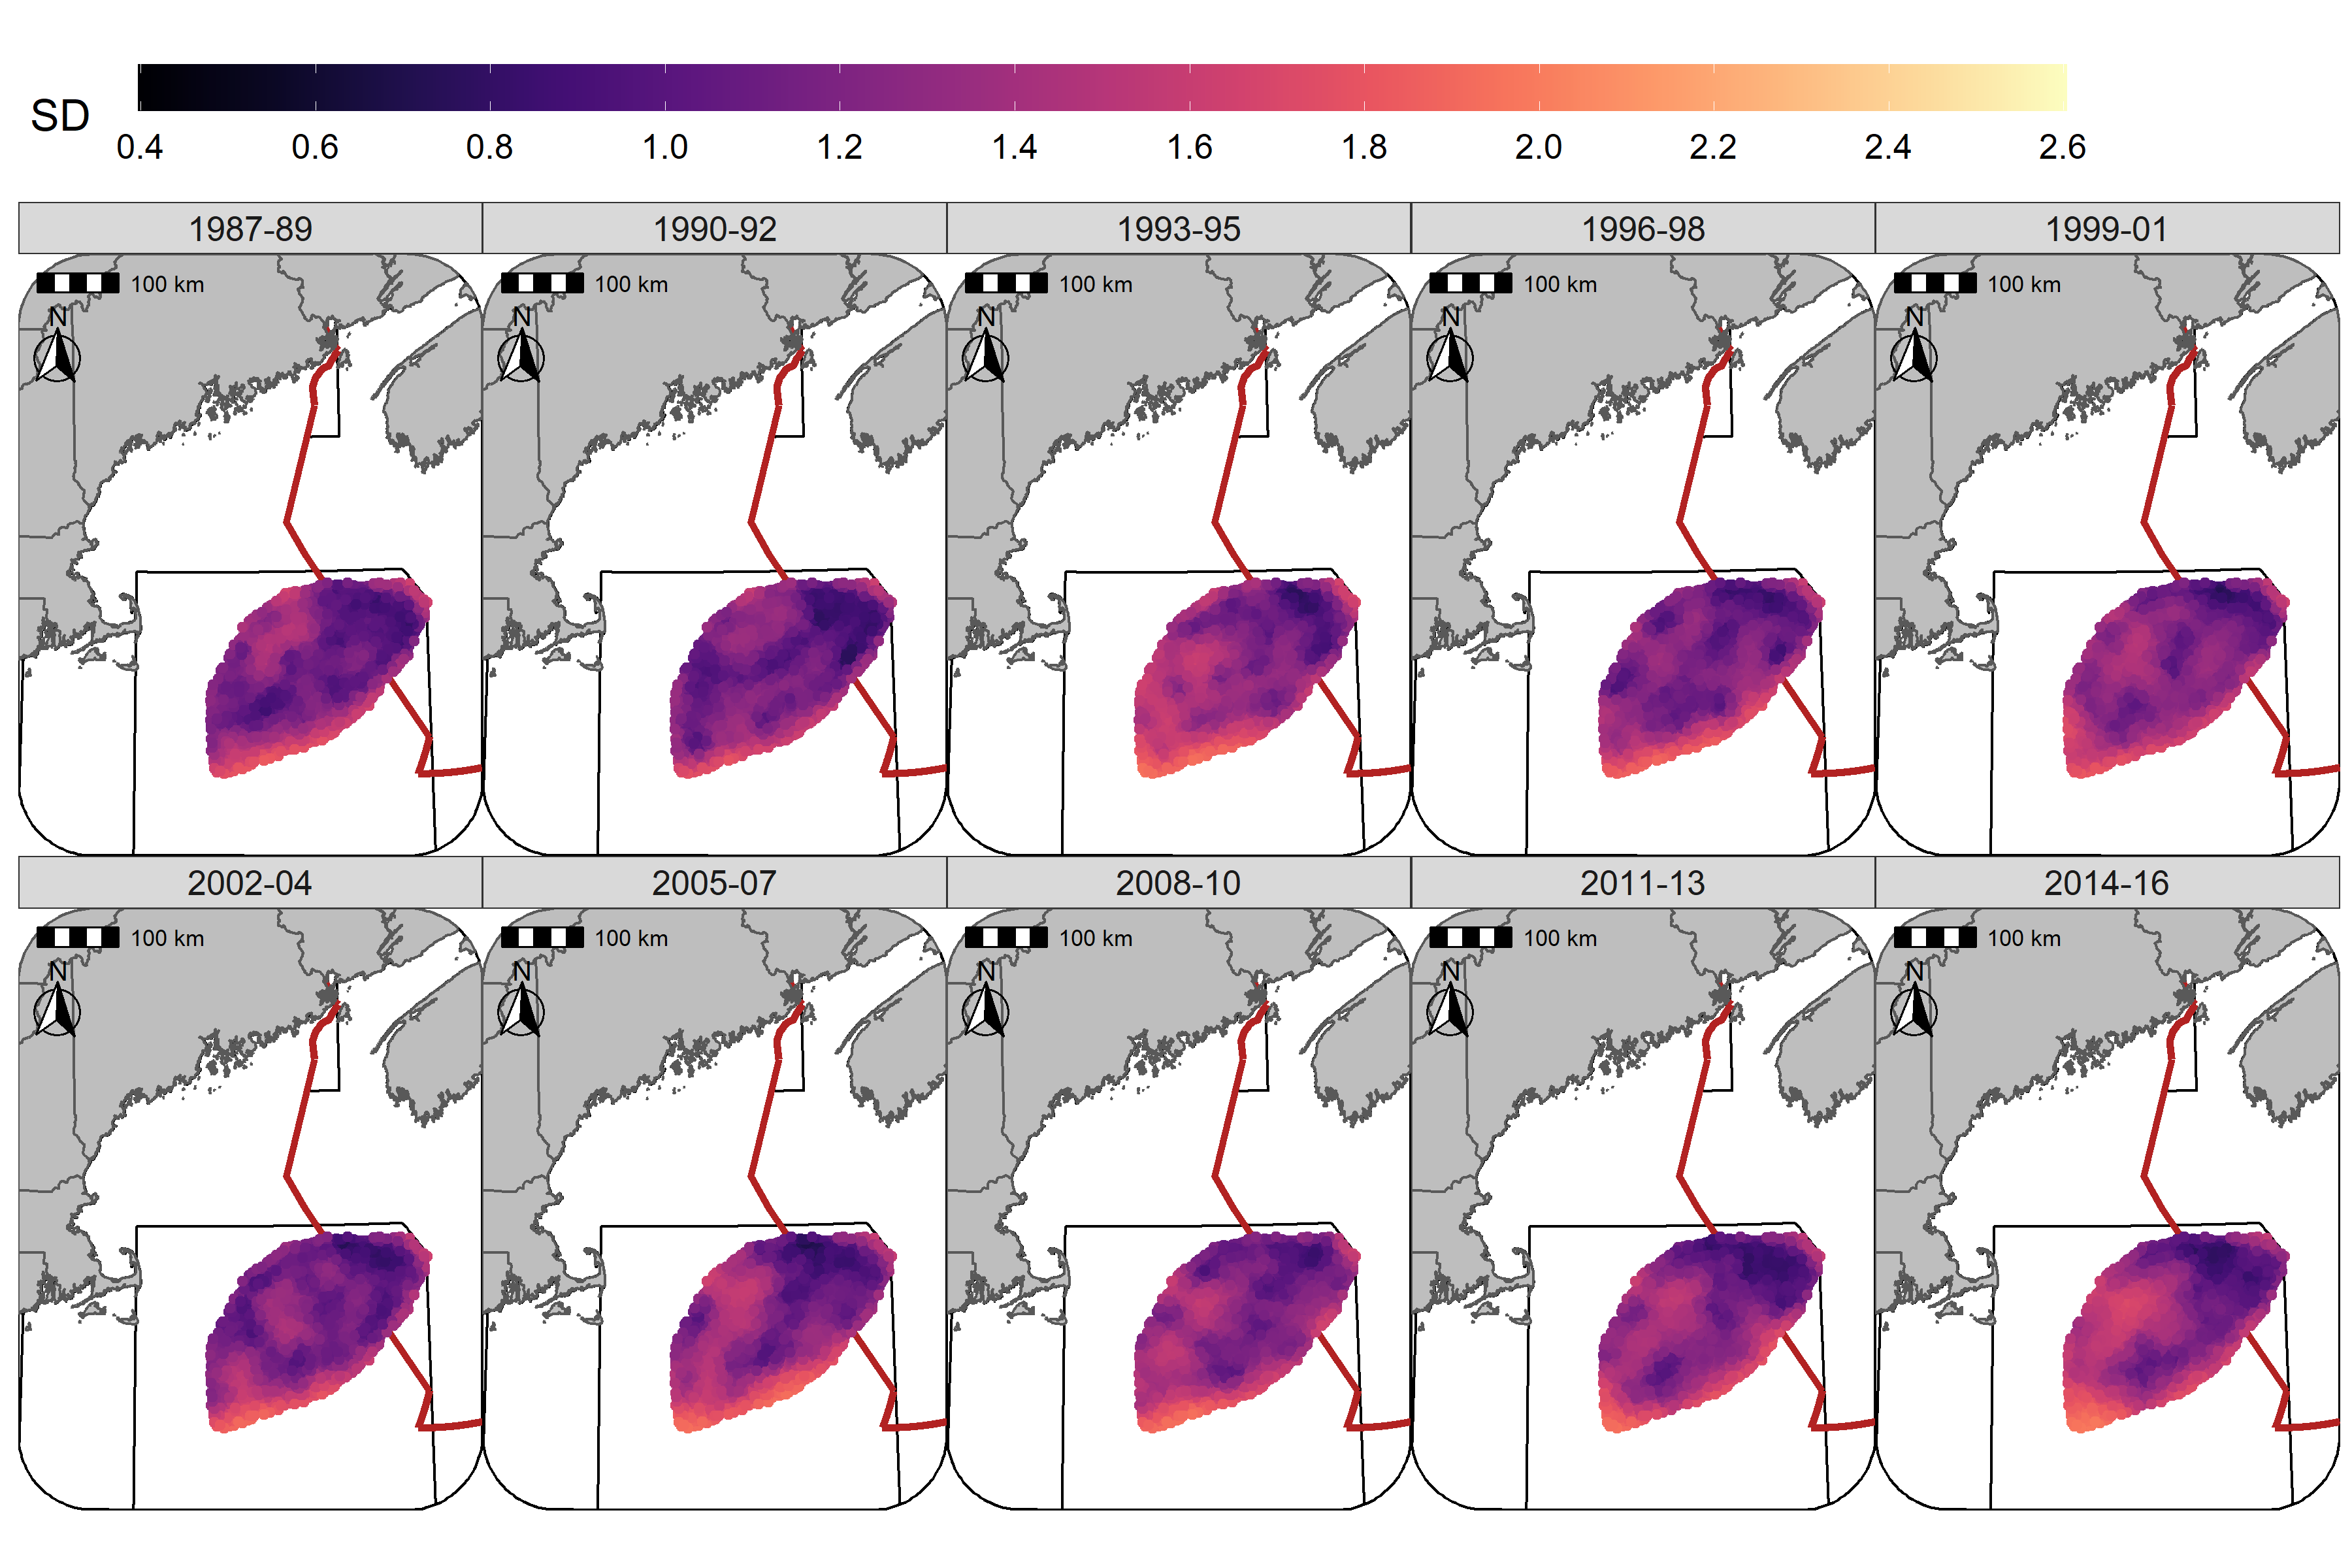
\includegraphics[width=1\linewidth]{D:/Github/Paper_2_SDMs/Results/Figures/rf_winter_yt_sd} 

}

\caption{Standard deviation of random fields (logit scale) for Yellowtail Flounder in each era during the Winter (RV survey) using the SST + Depth + Sed model and 3 year random field.}\label{fig:rf-winter-yt-sd}
\end{figure}

\newpage
\begin{figure}[htb]

{\centering 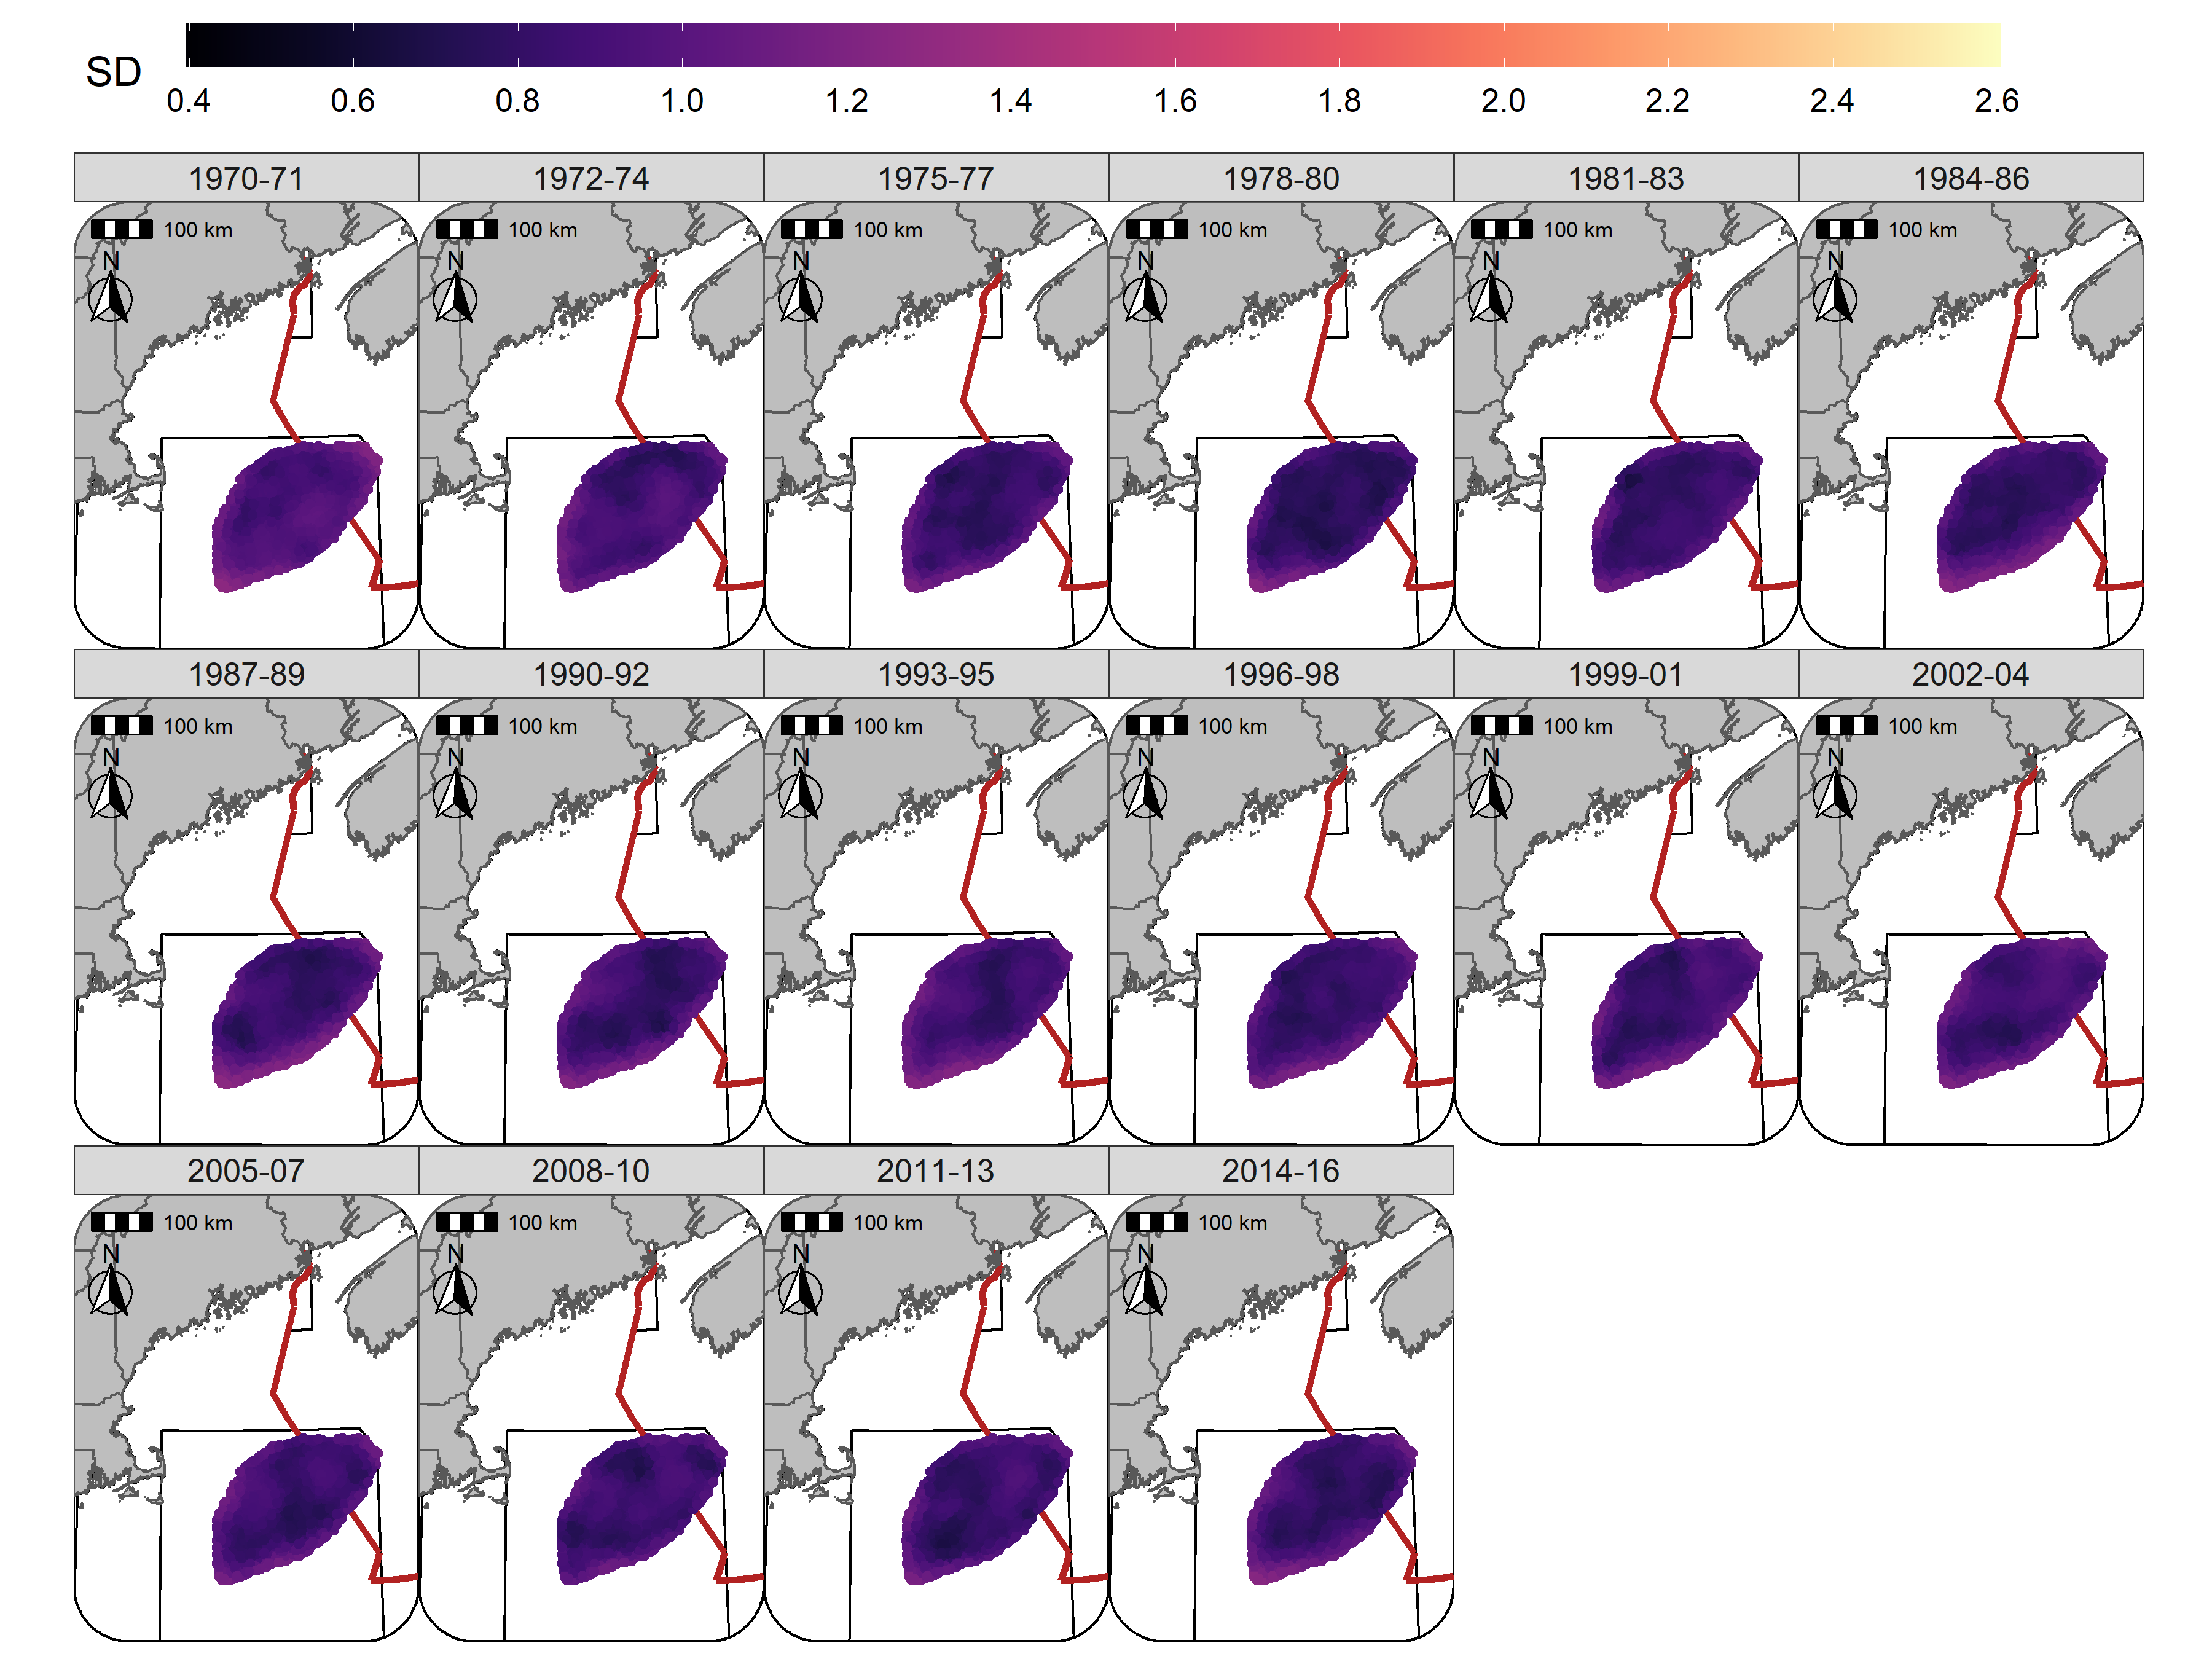
\includegraphics[width=1\linewidth]{D:/Github/Paper_2_SDMs/Results/Figures/rf_spring_yt_sd} 

}

\caption{Standard deviation of random fields (logit scale) for Yellowtail Flounder in each era during the Spring (NMFS-spring survey) using the SST + Depth + Sed model and 3 year random field.}\label{fig:rf-spring-yt-sd}
\end{figure}

\newpage
\begin{figure}[htb]

{\centering 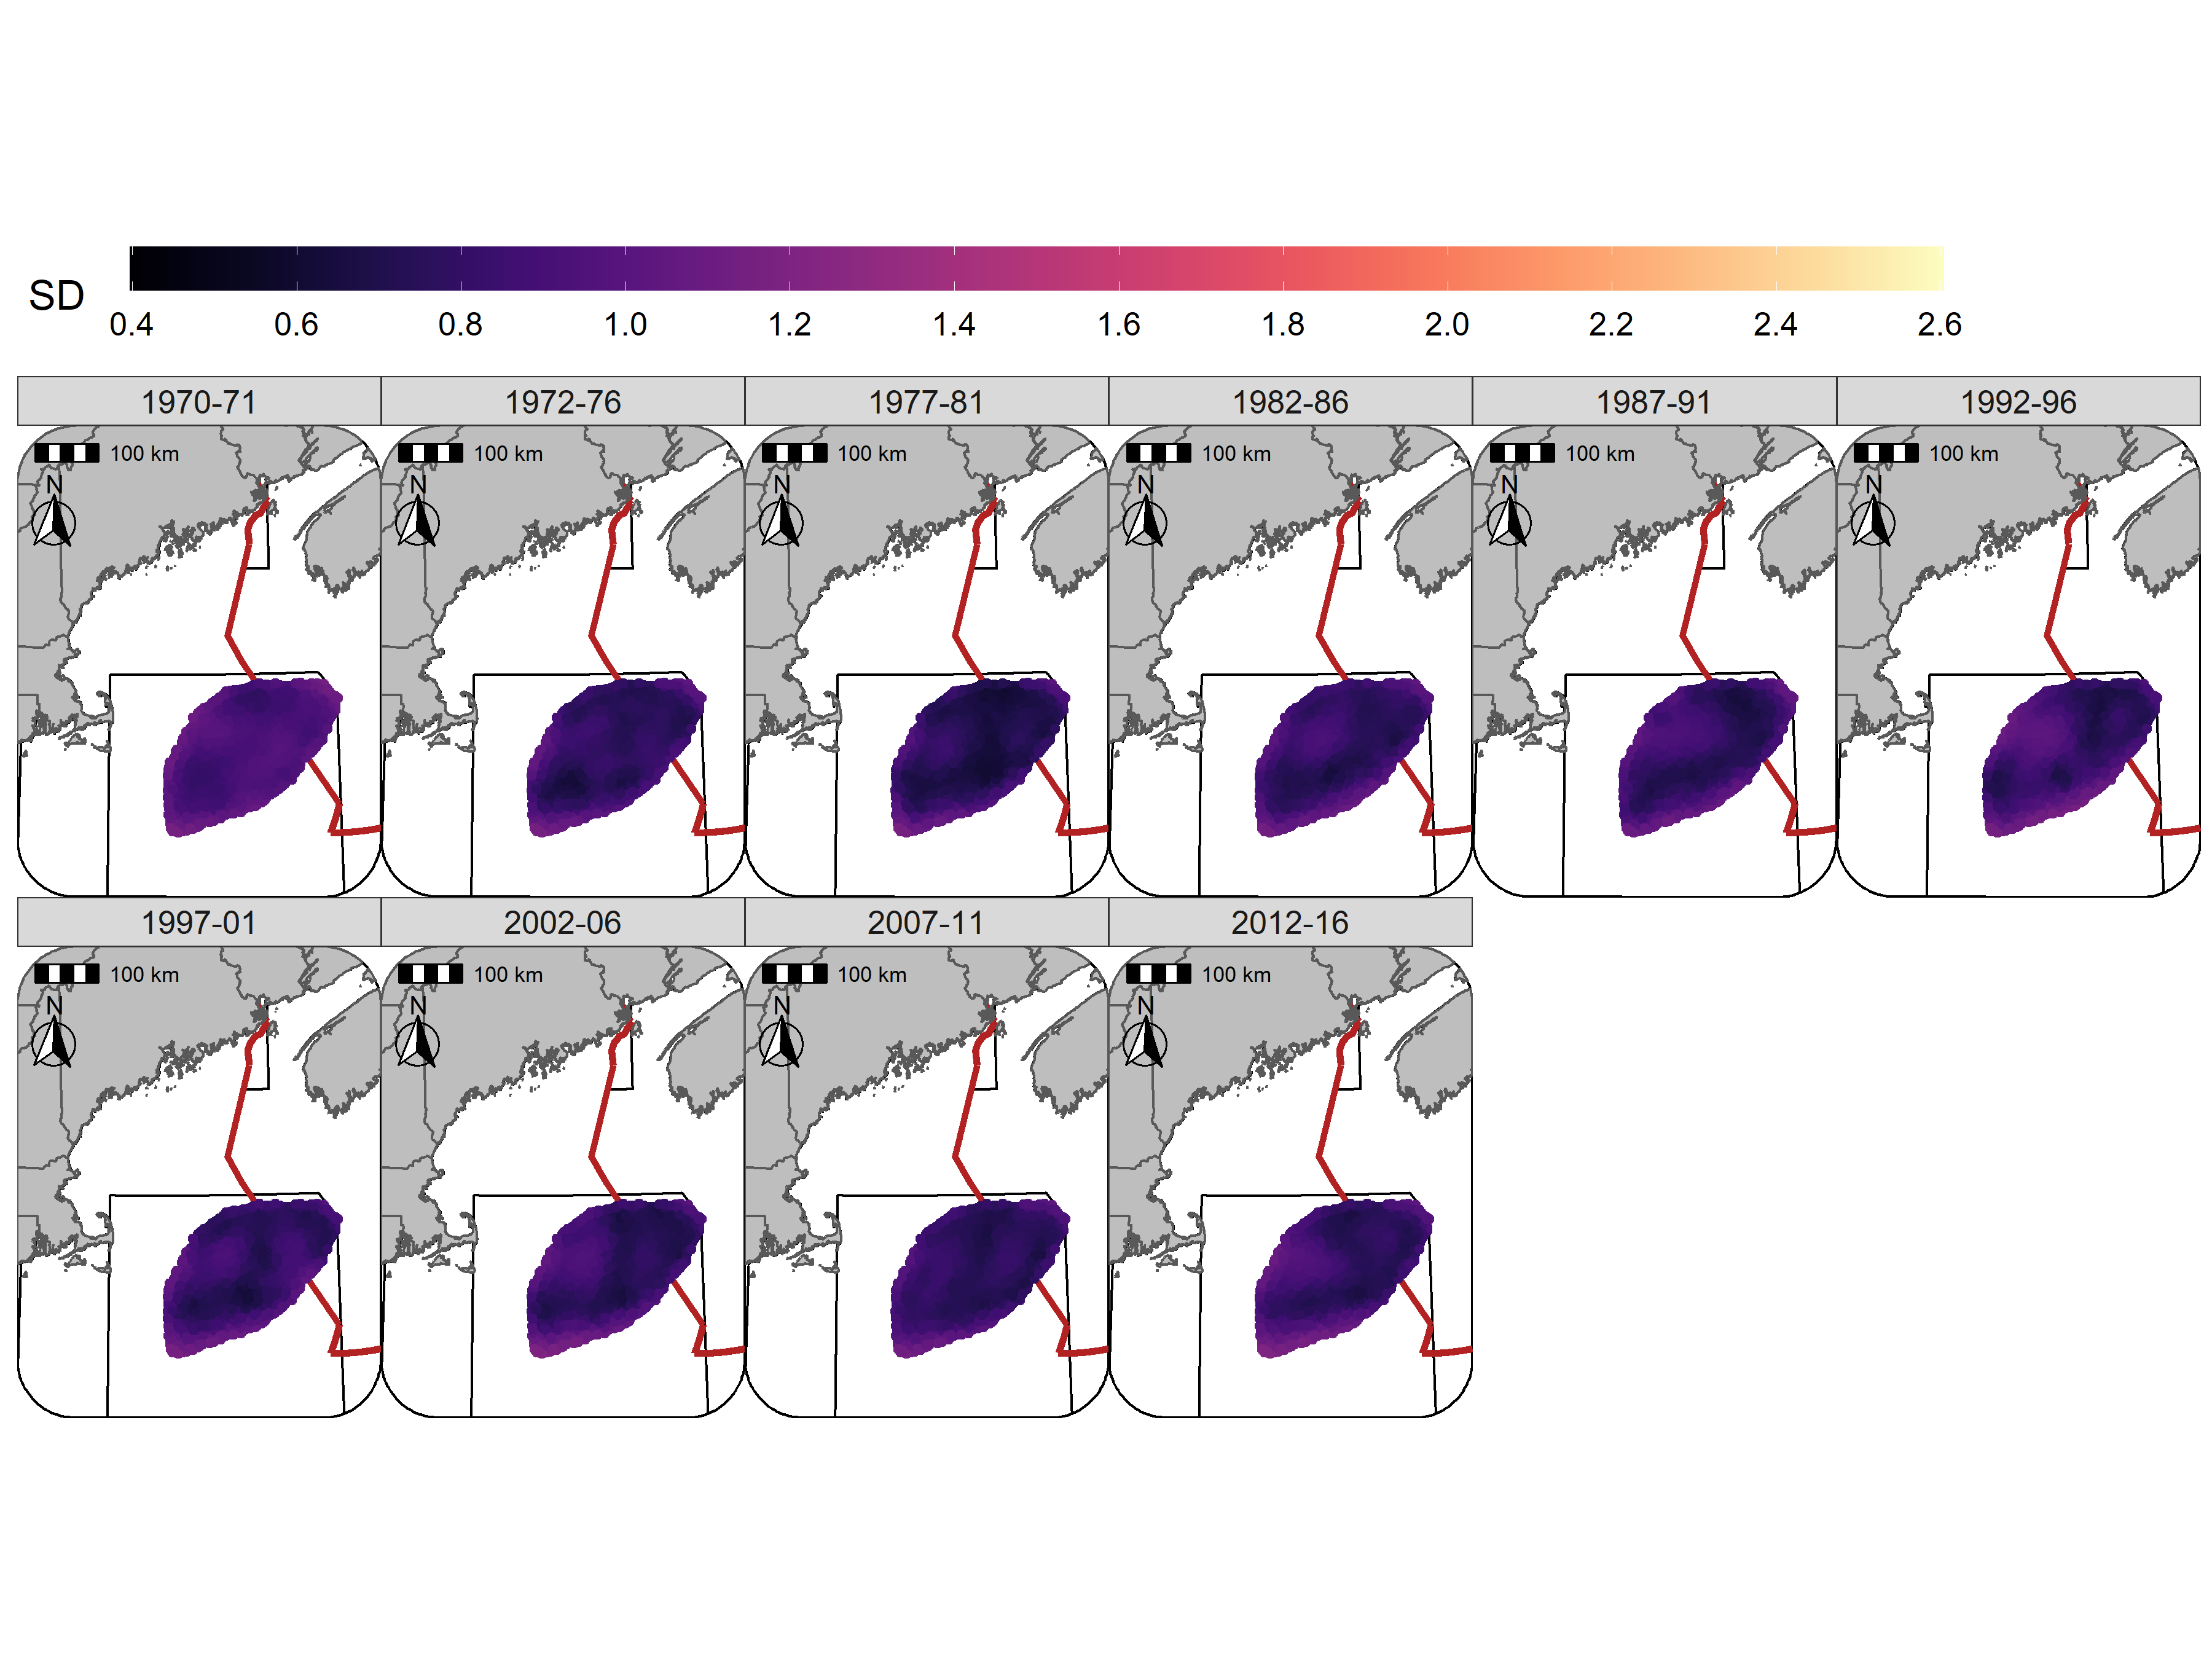
\includegraphics[width=1\linewidth]{D:/Github/Paper_2_SDMs/Results/Figures/rf_fall_yt_sd} 

}

\caption{Standard deviation of random fields (logit scale) for Yellowtail Flounder in each era during the Fall (NMFS-fall survey) using the SST + Depth + Sed model and 5 year random field.}\label{fig:rf-fall-yt-sd}
\end{figure}
\end{landscape}

\hypertarget{hyperparameters}{%
\subsection{Hyperparameters}\label{hyperparameters}}

For Atlantic Cod, the estimate for the variance of \emph{Dep} variance hyperparameter was highest in Winter and declined through to the Fall, reflecting the decline in the influence of this covariate in the Fall (Figure \ref{fig:hyper-dep-var-est}). For Yellowtail Flounder, the variance of the \emph{Dep} hyperparameter was higher than observed for Atlantic Cod throughout the year and reflected the relative stability in the effect size of this covariate throughout the year (Figure \ref{fig:hyper-dep-var-est}). The \emph{SST} variance hyperparameter for Atlantic Cod was relatively stable throughout the year and reflects the consistent influence of the \emph{SST} covariate on the distribution of cod. For Yellowtail Flounder, the \emph{SST} variance hyperparameter was relatively low throughout the year and aligns with the consistent small effect of the \emph{SST} covariate on the distribution of Yellowtail Flounder (Figure \ref{fig:hyper-sst-var-est}). The uncertainty of these estimates precludes any statistical differences being observed between the seasons.

\begin{figure}[htb]

{\centering \includegraphics[width=1\linewidth]{D:/Github/Paper_2_SDMs/Results/Figures/hyper_dep_var_est} 

}

\caption{Depth variance hyperparameter estimate with 95\%CI's for each stock in each season.}\label{fig:hyper-dep-var-est}
\end{figure}

\clearpage

\begin{figure}[htb]

{\centering \includegraphics[width=1\linewidth]{D:/Github/Paper_2_SDMs/Results/Figures/hyper_sst_var_est} 

}

\caption{*SST* variance hyperparameter estimate with 95\%CI's for each stock in each season.}\label{fig:hyper-sst-var-est}
\end{figure}

\clearpage

\begin{figure}[htb]

{\centering \includegraphics[width=1\linewidth]{D:/Github/Paper_2_SDMs/Results/Figures/cod_winter_marginal} 

}

\caption{Posteriors distributions of the four model hyperparameters for Atlantic Cod in the Winter.}\label{fig:hyper-cod-winter-post}
\end{figure}

\clearpage

\begin{figure}[htb]

{\centering \includegraphics[width=1\linewidth]{D:/Github/Paper_2_SDMs/Results/Figures/cod_spring_marginal} 

}

\caption{Posteriors distributions of the four model hyperparameters for Atlantic Cod in the Spring.}\label{fig:hyper-cod-spring-post}
\end{figure}

\clearpage

\begin{figure}[htb]

{\centering \includegraphics[width=1\linewidth]{D:/Github/Paper_2_SDMs/Results/Figures/cod_fall_marginal} 

}

\caption{Posteriors distributions of the four model hyperparameters for Atlantic Cod  in the Fall.}\label{fig:hyper-cod-fall-post}
\end{figure}

\clearpage

\begin{figure}[htb]

{\centering \includegraphics[width=1\linewidth]{D:/Github/Paper_2_SDMs/Results/Figures/yt_winter_marginal} 

}

\caption{Posteriors distributions of the four model hyperparameters for Yellowtail Flounder in the Winter.}\label{fig:hyper-yt-winter-post}
\end{figure}

\clearpage

\begin{figure}[htb]

{\centering \includegraphics[width=1\linewidth]{D:/Github/Paper_2_SDMs/Results/Figures/yt_spring_marginal} 

}

\caption{Posteriors distributions of the four model hyperparameters for Yellowtail Flounder in the Spring.}\label{fig:hyper-yt-spring-post}
\end{figure}

\clearpage

\begin{figure}[htb]

{\centering \includegraphics[width=1\linewidth]{D:/Github/Paper_2_SDMs/Results/Figures/yt_fall_marginal} 

}

\caption{Posteriors distributions of the four model hyperparameters for Yellowtail Flounder in the Fall.}\label{fig:hyper-yt-fall-post}
\end{figure}

\clearpage

\end{document}
